\documentclass{beamer}

% xcolor and define colors -------------------------
\usepackage{xcolor}

% https://www.viget.com/articles/color-contrast/
\definecolor{purple}{HTML}{5601A4}
\definecolor{navy}{HTML}{0D3D56}
\definecolor{ruby}{HTML}{9a2515}
\definecolor{alice}{HTML}{107895}
\definecolor{daisy}{HTML}{EBC944}
\definecolor{coral}{HTML}{F26D21}
\definecolor{kelly}{HTML}{829356}
\definecolor{cranberry}{HTML}{E64173}
\definecolor{jet}{HTML}{131516}
\definecolor{asher}{HTML}{555F61}
\definecolor{slate}{HTML}{314F4F}

% Mixtape Sessions
\definecolor{picton-blue}{HTML}{00b7ff}
\definecolor{violet-red}{HTML}{ff3881}
\definecolor{sun}{HTML}{ffaf18}
\definecolor{electric-violet}{HTML}{871EFF}

% Main theme colors
\definecolor{accent}{HTML}{00b7ff}
\definecolor{accent2}{HTML}{871EFF}
\definecolor{gray100}{HTML}{f3f4f6}
\definecolor{gray800}{HTML}{1F292D}


% Beamer Options -------------------------------------

% Background
\setbeamercolor{background canvas}{bg = white}

% Change text margins
\setbeamersize{text margin left = 15pt, text margin right = 15pt} 

% \alert
\setbeamercolor{alerted text}{fg = accent2}

% Frame title
\setbeamercolor{frametitle}{bg = white, fg = jet}
\setbeamercolor{framesubtitle}{bg = white, fg = accent}
\setbeamerfont{framesubtitle}{size = \small, shape = \itshape}

% Block
\setbeamercolor{block title}{fg = white, bg = accent2}
\setbeamercolor{block body}{fg = gray800, bg = gray100}

% Title page
\setbeamercolor{title}{fg = gray800}
\setbeamercolor{subtitle}{fg = accent}

%% Custom \maketitle and \titlepage
\setbeamertemplate{title page}
{
    %\begin{centering}
        \vspace{20mm}
        {\Large \usebeamerfont{title}\usebeamercolor[fg]{title}\inserttitle}\\
        {\large \itshape \usebeamerfont{subtitle}\usebeamercolor[fg]{subtitle}\insertsubtitle}\\ \vspace{10mm}
        {\insertauthor}\\
        {\color{asher}\small{\insertdate}}\\
    %\end{centering}
}

% Table of Contents
\setbeamercolor{section in toc}{fg = accent!70!jet}
\setbeamercolor{subsection in toc}{fg = jet}

% Button 
\setbeamercolor{button}{bg = accent}

% Remove navigation symbols
\setbeamertemplate{navigation symbols}{}

% Table and Figure captions
\setbeamercolor{caption}{fg=jet!70!white}
\setbeamercolor{caption name}{fg=jet}
\setbeamerfont{caption name}{shape = \itshape}

% Bullet points

%% Fix left-margins
\settowidth{\leftmargini}{\usebeamertemplate{itemize item}}
\addtolength{\leftmargini}{\labelsep}

%% enumerate item color
\setbeamercolor{enumerate item}{fg = accent}
\setbeamerfont{enumerate item}{size = \small}
\setbeamertemplate{enumerate item}{\insertenumlabel.}

%% itemize
\setbeamercolor{itemize item}{fg = accent!70!white}
\setbeamerfont{itemize item}{size = \small}
\setbeamertemplate{itemize item}[circle]

%% right arrow for subitems
\setbeamercolor{itemize subitem}{fg = accent!60!white}
\setbeamerfont{itemize subitem}{size = \small}
\setbeamertemplate{itemize subitem}{$\rightarrow$}

\setbeamertemplate{itemize subsubitem}[square]
\setbeamercolor{itemize subsubitem}{fg = jet}
\setbeamerfont{itemize subsubitem}{size = \small}


% Special characters

\usepackage{collectbox}

\makeatletter
\newcommand{\mybox}{%
    \collectbox{%
        \setlength{\fboxsep}{1pt}%
        \fbox{\BOXCONTENT}%
    }%
}
\makeatother





% Links ----------------------------------------------

\usepackage{hyperref}
\hypersetup{
  colorlinks = true,
  linkcolor = accent2,
  filecolor = accent2,
  urlcolor = accent2,
  citecolor = accent2,
}


% Line spacing --------------------------------------
\usepackage{setspace}
\setstretch{1.1}


% \begin{columns} -----------------------------------
\usepackage{multicol}


% Fonts ---------------------------------------------
% Beamer Option to use custom fonts
\usefonttheme{professionalfonts}

% \usepackage[utopia, smallerops, varg]{newtxmath}
% \usepackage{utopia}
\usepackage[sfdefault,light]{roboto}

% Small adjustments to text kerning
\usepackage{microtype}



% Remove annoying over-full box warnings -----------
\vfuzz2pt 
\hfuzz2pt


% Table of Contents with Sections
\setbeamerfont{myTOC}{series=\bfseries, size=\Large}
\AtBeginSection[]{
        \frame{
            \frametitle{Roadmap}
            \tableofcontents[current]   
        }
    }


% Tables -------------------------------------------
% Tables too big
% \begin{adjustbox}{width = 1.2\textwidth, center}
\usepackage{adjustbox}
\usepackage{array}
\usepackage{threeparttable, booktabs, adjustbox}
    
% Fix \input with tables
% \input fails when \\ is at end of external .tex file
\makeatletter
\let\input\@@input
\makeatother

% Tables too narrow
% \begin{tabularx}{\linewidth}{cols}
% col-types: X - center, L - left, R -right
% Relative scale: >{\hsize=.8\hsize}X/L/R
\usepackage{tabularx}
\newcolumntype{L}{>{\raggedright\arraybackslash}X}
\newcolumntype{R}{>{\raggedleft\arraybackslash}X}
\newcolumntype{C}{>{\centering\arraybackslash}X}

% Figures

% \imageframe{img_name} -----------------------------
% from https://github.com/mattjetwell/cousteau
\newcommand{\imageframe}[1]{%
    \begin{frame}[plain]
        \begin{tikzpicture}[remember picture, overlay]
            \node[at = (current page.center), xshift = 0cm] (cover) {%
                \includegraphics[keepaspectratio, width=\paperwidth, height=\paperheight]{#1}
            };
        \end{tikzpicture}
    \end{frame}%
}

% subfigures
\usepackage{subfigure}


% Highlight slide -----------------------------------
% \begin{transitionframe} Text \end{transitionframe}
% from paulgp's beamer tips
\newenvironment{transitionframe}{
    \setbeamercolor{background canvas}{bg=accent!40!black}
    \begin{frame}\color{accent!10!white}\LARGE\centering
}{
    \end{frame}
}


% Table Highlighting --------------------------------
% Create top-left and bottom-right markets in tabular cells with a unique matching id and these commands will outline those cells
\usepackage[beamer,customcolors]{hf-tikz}
\usetikzlibrary{calc}
\usetikzlibrary{fit,shapes.misc}

% To set the hypothesis highlighting boxes red.
\newcommand\marktopleft[1]{%
    \tikz[overlay,remember picture] 
        \node (marker-#1-a) at (0,1.5ex) {};%
}
\newcommand\markbottomright[1]{%
    \tikz[overlay,remember picture] 
        \node (marker-#1-b) at (0,0) {};%
    \tikz[accent!80!jet, ultra thick, overlay, remember picture, inner sep=4pt]
        \node[draw, rectangle, fit=(marker-#1-a.center) (marker-#1-b.center)] {};%
}

\usepackage{breqn} % Breaks lines

\usepackage{amsmath}
\usepackage{mathtools}

\usepackage{pdfpages} % \includepdf

\usepackage{listings} % R code
\usepackage{verbatim} % verbatim

% Video stuff
\usepackage{media9}

% packages for bibs and cites
\usepackage{natbib}
\usepackage{har2nat}
\newcommand{\possessivecite}[1]{\citeauthor{#1}'s \citeyearpar{#1}}
\usepackage{breakcites}
\usepackage{alltt}

% tikz
\usepackage{tikz}
\usepackage{pgfplots}
\usetikzlibrary{calc, positioning, decorations.pathreplacing, arrows.meta, intersections}
\pgfdeclarelayer{bg}
\pgfdeclarelayer{back}
\pgfdeclarelayer{fg}
\pgfsetlayers{bg,main,fg,back}
\usetikzlibrary{shapes,arrows}

% Setup math operators
\DeclareMathOperator{\E}{E} \DeclareMathOperator{\tr}{tr} \DeclareMathOperator{\se}{se} \DeclareMathOperator{\I}{I} \DeclareMathOperator{\sign}{sign} \DeclareMathOperator{\supp}{supp} \DeclareMathOperator{\plim}{plim}
\DeclareMathOperator*{\dlim}{\mathnormal{d}\mkern2mu-lim}
\newcommand\independent{\protect\mathpalette{\protect\independenT}{\perp}}
   \def\independenT#1#2{\mathrel{\rlap{$#1#2$}\mkern2mu{#1#2}}}
\newcommand*\colvec[1]{\begin{pmatrix}#1\end{pmatrix}}

\newcommand{\myurlshort}[2]{\href{#1}{\textcolor{gray}{\textsf{#2}}}}


\begin{document}

\imageframe{./lecture_includes/mixtape_did_cover.png}


% ---- Content ----

\section{In Pursuit of the ATT}




\begin{frame}{Welcome!}

  \begin{itemize}
	\item Scott Cunningham, professor of economics at Baylor University, author of \underline{Causal Inference: the Mixtape}
	\item Identifying the causal parameter, ATT, using unconfoundedness and synthetic control (maybe diff-in-diff)
	\item Deep dive into the potential outcomes framework, which is surprisingly powerful as notation for causal inference when combined with modern statistics

  \end{itemize}

\end{frame}



\begin{frame}{What my pedagogy is like}

\begin{itemize}
\item Long day that don't feel long because it's high energy, with regular breaks including lunch
\item Move between the econometrics, history of thought, videos, applications, code, spreadsheets, exercises
\item Ask questions at any point; I'll do my best to answer them
\end{itemize}

\end{frame}



\begin{frame}{Outline}

  \begin{enumerate}
    \item Potential outcomes and the ATT
    \item Selection Bias, Treatment Assignment and Randomization
    \item Unconfoundedness, Regression, Matching and Propensity Score Weighting
    \item Synthetic control with and without negative weighting
    \item Difference-in-differences, covariates and staggered roll out (if time, but likely won't be)
  \end{enumerate}

\end{frame}



\subsection{Potential Outcomes}

\begin{frame}{Mandatory Spurious Correlation Slide}
  \centering
  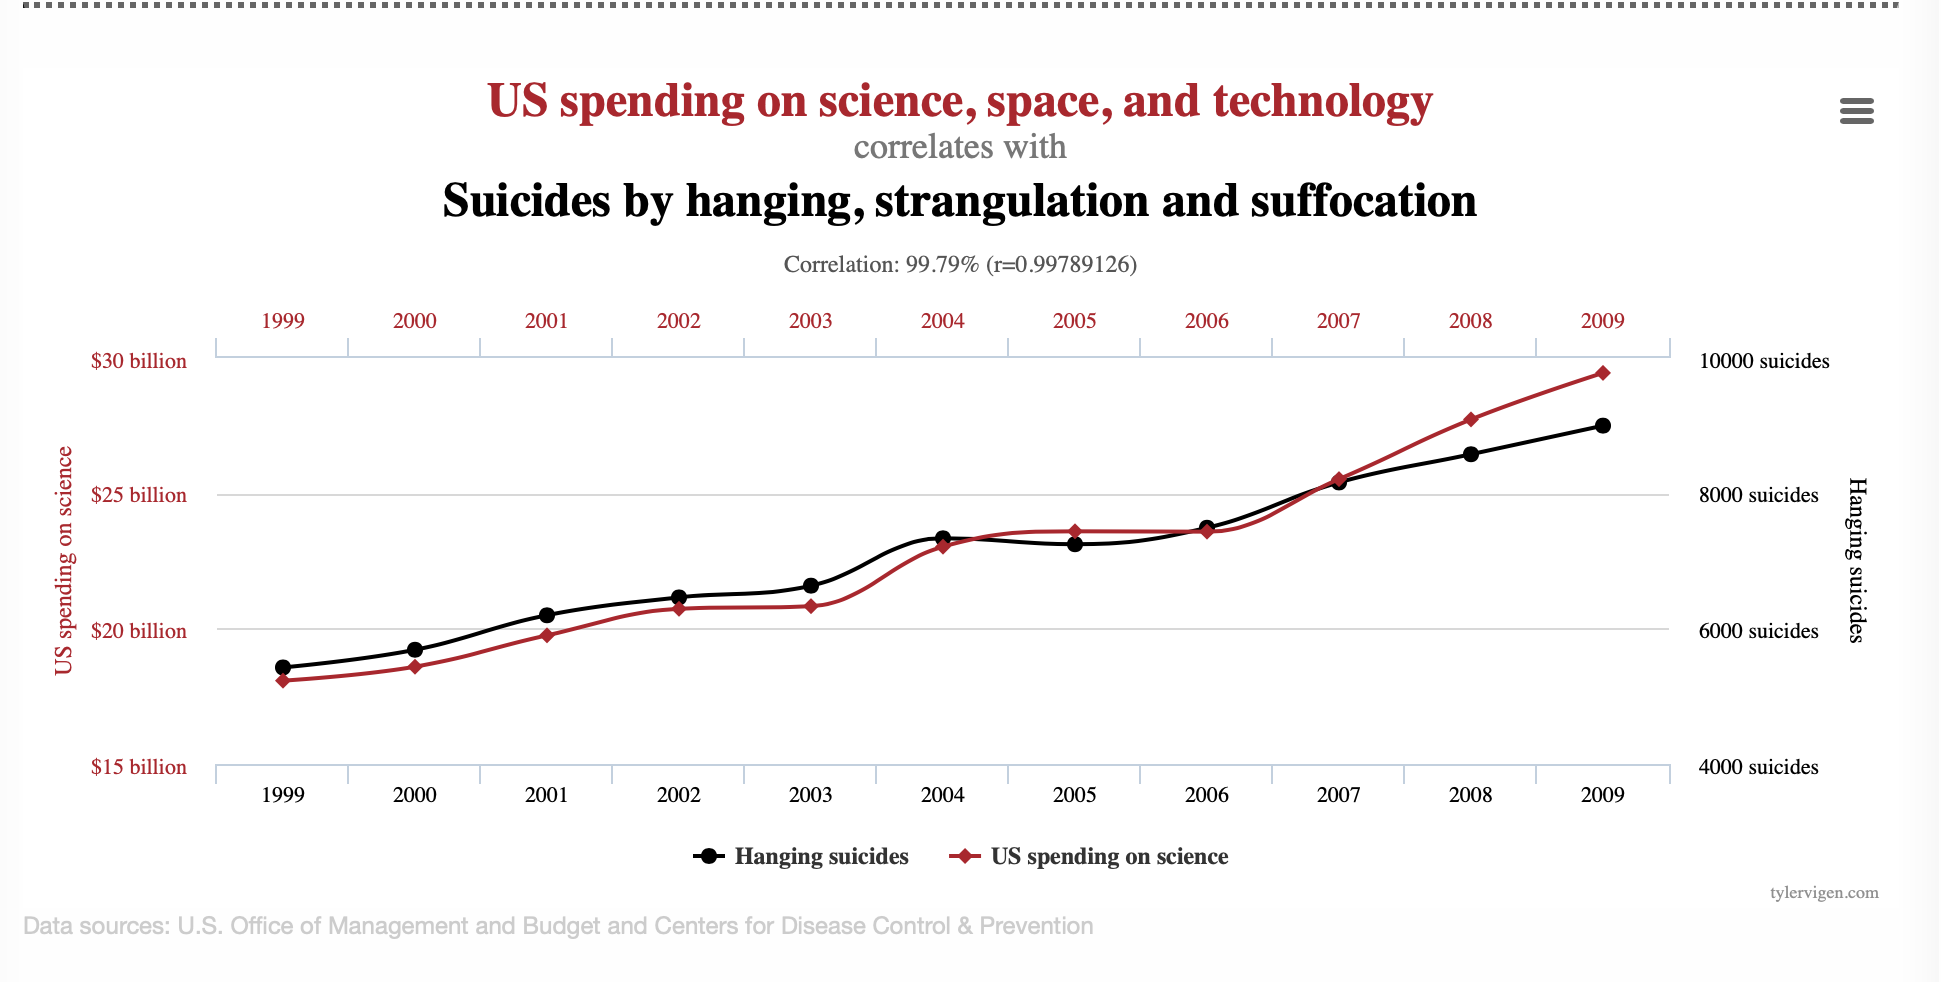
\includegraphics[scale=0.5,height=6.5cm, width=10cm]{./lecture_includes/spurious_correlation}
\end{frame}

\begin{frame}{What is Causality?}

\begin{itemize}
\item Causality is metaphysics; causal inference is epistemology -- what makes a causal belief a ``warranted belief''?
\item Causal inference has many mothers and fathers
\item Aristotle was different than Hume, Mill, and Lewis and as I am not comfortable saying Aristotle was wrong, I won't
\item What I can do is explain the potential outcomes framework of causal inference and use it to discuss methods and tools that estimate unbiased and meaningful causal parameters as defined by that framework
\end{itemize}

\end{frame}


\begin{frame}{Causal Inference vs Prediction}
  \centering
  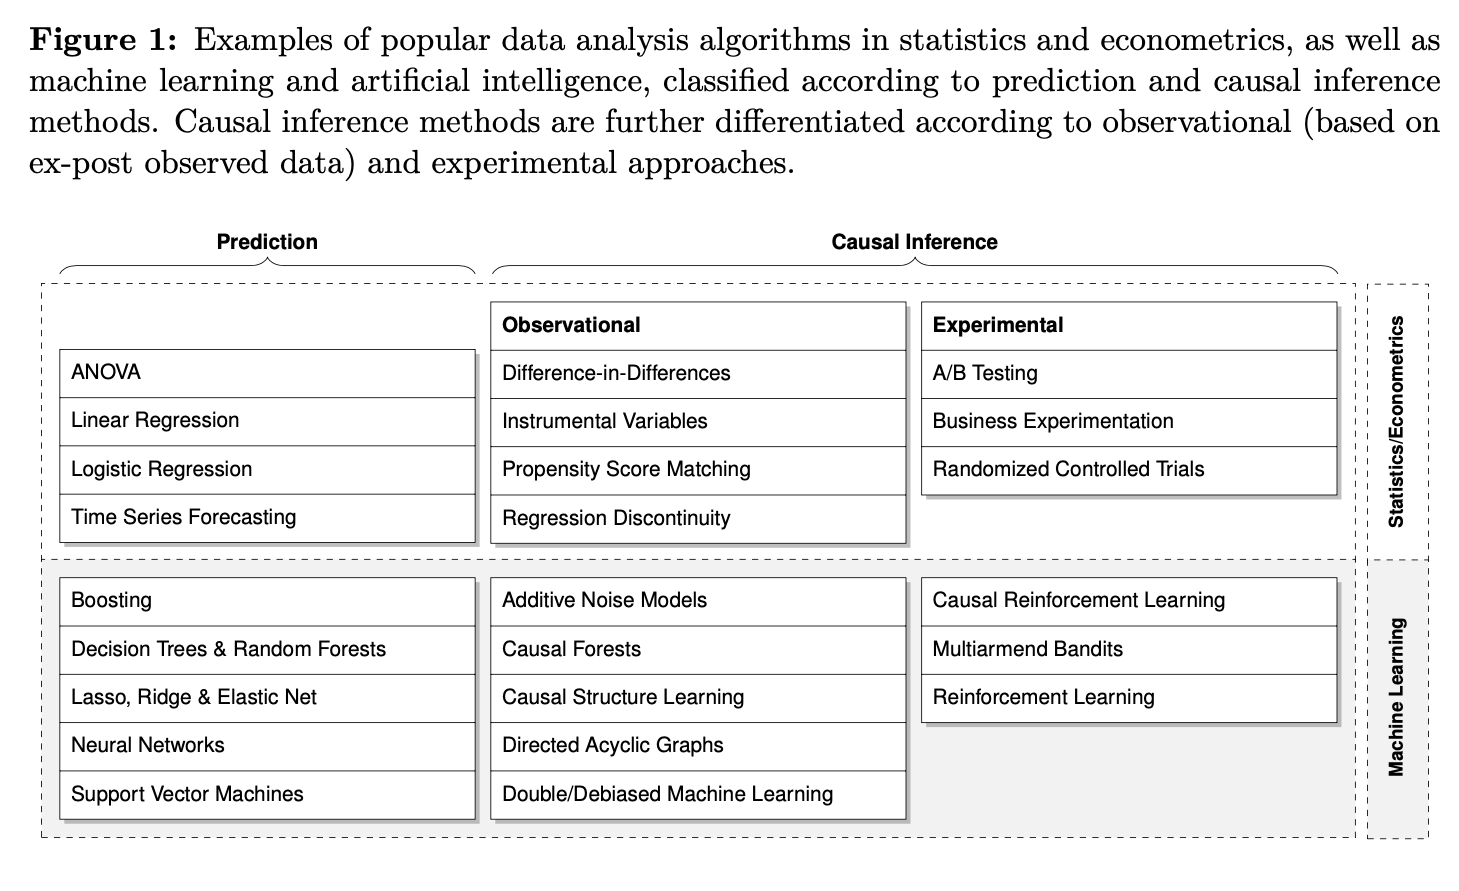
\includegraphics[scale=0.5,height=6.5cm, width=10cm]{./lecture_includes/prediction_causality.png}
\end{frame}

\begin{frame}{Causal Inference vs Prediction}

  \begin{columns}
    \column{0.48\linewidth}
    \centering
    \textbf{Traditional prediction}
    \begin{itemize}
      \item Traditional prediction seeks to detect patterns in data and fit functional relationships between variables with a high degree of accuracy
      \item ``Does this person have heart disease?'', ``How many books will I sell?''
      \item It is not predictions of what effect a choice will have, though
    \end{itemize}
    \column{0.48\linewidth}
    \centering
    \textbf{Causal inference}
    \begin{itemize}
      \item Causal inference is also a type of prediction, but it's a prediction of a \emph{counterfactual} associated with a particular \emph{choice taken}
      \item Causal inference takes that predicted (or imputed) counterfactual and constructs a causal effect that we hope tells us about a future in the event of a similar choice taken
    \end{itemize}
  \end{columns}
\end{frame}



\begin{frame}{Naive causal inference}

  \begin{itemize}
    \item Aliens estimate a model showing a systematic correlation between COVID deaths and ventilators
    \item They conclude doctors are killing patients with ventilators so they come to earth to liberate the patients, but it only makes things worse
    \item Their error was they confused correlation with causality, but deeper than that, they didn't understand how the world worked
    \item \emph{We are the aliens in our research}
  \end{itemize}

\end{frame}

\begin{frame}{\#1: Correlation and causality are different concepts}

  Causal is one unit, correlation is many units
  \begin{itemize}
    \item Causal question: ``If a doctor puts a patient on a ventilator (D), will her covid symptoms (Y) improve?''
    \item Correlation question:  $$\frac{Cov(D,Y)}{\sqrt{Var_D}\sqrt{{Var_Y}}}$$
    \item Error extends to predictive modeling that isn't based on causal frameworks
  \end{itemize}

\end{frame}



\begin{frame}{\#2: Coming first may not mean causality!}

  \begin{itemize}
    \item Every morning the rooster crows and then the sun rises
    \item Did the rooster cause the sun to rise? Or did the sun cause the rooster to crow?
    \item What if cat killed the rooster?
    \item \emph{Post hoc ergo propter hoc}: ``after this, therefore, because of this''
  \end{itemize}

\end{frame}

\begin{frame}{\#3: Causality may mask correlations!}

  \begin{figure}
    \centering
    \includegraphics[scale=0.04]{./lecture_includes/scottboat.jpg}
  \end{figure}

\end{frame}


\begin{frame}{Modeling is Not the First Step}

Most of us simply estimate models and cross our fingers that that coefficient is causal, but is it? When is it?  Why is it? And which causal effect is it?  And when is it reasonable to believe it? 

\bigskip

We have to introduce concepts and notation first otherwise we will extend the correlation fallacy


\end{frame}



\begin{frame}{Three New Ideas}

\begin{enumerate}
\item \textbf{Counterfactual}: Philosophers come to it first and its central role in causal inference makes causality \emph{unknowable} that the project is nearly derailed
\item \textbf{Treatment assignment mechanism}: Neyman and Fisher solve the counterfactual problem in statistics and lay the foundation of the modern randomized controlled trial (RCT) with their focus on the selection process
\item \textbf{No One Causal Effect}: There is no such thing as``the causal effect''; there's many and your first step is to pick a parameter (not as easy as it sounds)
\end{enumerate}


\end{frame}


\begin{frame}{Definition and Identification Come First}

\begin{enumerate}
\item Turn the research question (``what is the causal effect of an advertising campaign on sales?'') into a specific aggregate causal parameter
\item Describe the narrow set of beliefs that make that parameter obtainable with data
\item Build a model that uses the data and the beliefs to estimate the causal parameter?
\end{enumerate}

\bigskip

Most of us skip (1) and many skip (2) and go straight to (3) but hopefully today I'll convince you that that's how errors are introduced, even after one understands that causal inference is not merely correlational

\end{frame}




\begin{frame}{Modern Philosophers Introduce Counterfactual Comparisons}

\begin{quote}
    ``If a person eats of a particular dish, and dies in consequence, that is, would not have died if he had not eaten it, people would be apt to say that eating of that dish was the source of his death.'' -- John Stuart Mill (19th century moral philosopher and economist)
\end{quote}

\bigskip
  
    \begin{quote}
    ``Causation is something that makes a difference, and the difference it makes must be a difference from what would have happened without it.'' -- David Lewis (20th century philosopher)
\end{quote}

\end{frame}

  
\begin{frame}{Counterfactuals Almost Derailed Causal Inference}



Mill's counterfactuals were immensely valuable for the clarity of the definition as well as its intuitive validity of causality, but it came at a huge price 

\bigskip

If I have to know what would have happened had I not eaten the dish, but I did eat the dish, then isn't it actually impossible to know the causal effect of eating the dish?

\bigskip

Statisticians surprisingly resolve this tension in the early 20th century with the introduction of notation and the principles of treatment assignment


\end{frame}


\begin{frame}{Statistical origins}

\begin{quote}
``Yet, although the seeds of the idea that [causal effects are comparisons of potential outcomes] can be traced back at least to the 18th century [most likely he means David Hume], the formal notation for potential outcomes was not introduced until 1923 by Neyman.'' -- Don Rubin (1990)
\end{quote}

\end{frame}


\begin{frame}{Jerzy Neyman's Notation}

\begin{itemize}
\item Jerzy Neyman's 1923 article describes a field experiment with differing plots of land (imagine hundreds of square gardens) and many different ``varieties'' of fertilizer that farmers could apply to the land
\item ``$U_{ik}$ is the yield of the $i$th variety on the $k$th plot...'' (Neyman 1923)
\item He calls $U_{ik}$ ``potential yield'', as opposed to the realized yield because $i$ (the fertilizer type) described all possible fertilizers that could be assigned to each $k$ square garden
\item Though only one fertilizer will be assigned to the land, many possible fertilizer assignments were possible beforehand, each with their own outcome
\end{itemize}

\end{frame}

\begin{frame}{Jerzy Neyman's Notation}

\begin{itemize}

\item For each fertilizer there is an associated ``potential yield'' that he collapses into $U$ which he considers to be ``a priori fixed but unknown'' (Rubin 1990)
\item Farmers draw fertilizer from an urn, like a bingo ball from a bingo ball machine, with replacement and apply it to each square garden
\item Fertilizer assignment moves us from ``all possible outcomes'' to ``realized outcome'' terminology
\item Neyman's urn model was a classic thought experiment, but it was also stochastically identical to the completely randomized experiment
\item His arch-rival, Ronald Fisher, realizes this and publishes a book two years later calling for \emph{randomizization} as the basis for causal inference
\end{itemize}

\end{frame}

\begin{frame}{Treatment assignment mechanism}

\begin{quote}

``Before the 20th century, there appears to have been only limited awareness of the concept of the assignment mechanism.  Although by the 1930s, randomized experiments were firmly established in some areas of scientific investigation, notably in agricultural experiments, there was no formal statement for a general assignment mechanism and, moreover, not even formal arguments in favor of randomization until Fisher (1925).'' (Imbens and Rubin 2015)

\end{quote}

\end{frame}

\begin{frame}{Progress is made and progress is not made}

\begin{itemize}

\item Econometrics traditionally modeled causality in terms of realized outcomes until recently (with some exceptions)
\item We need to make a distinction between now the idea of data (``realized outcomes'') and these hypothetical concepts represented by Neyman's notation (``potential outcomes'')
\item Listen to Guido Imbens describe the transition towards modeling causality in terms of ``realized outcomes''

\end{itemize}

\bigskip

\url{https://www.youtube.com/watch?v=drGkRy53bB4}

\end{frame}



\begin{frame}{Potential outcomes notation}

Let the treatment be a binary variable: $$D_{i,t} =\begin{cases} 1 \text{ if placed on ventilator at time $t$} \\ 0 \text{ if not placed on ventilator at time $t$} \end{cases}$$where $i$ indexes an individual observation, such as a person
\end{frame}

\begin{frame}{Potential outcomes notation}

Potential outcomes: $$Y_{i,t}^j =\begin{cases} 1 \text{ health if placed on ventilator at time $t$} \\ 0 \text{ health if not placed on ventilator at time $t$} \end{cases}$$where $j$ indexes a potential treatment status for the same $i$ person at the same $t$ point in time
\end{frame}


\begin{frame}{Realized vs potential outcomes}

  \begin{itemize}
    \item Potential outcome $Y^1$ refers to the ``a priori fixed but unknown'' outcomes associated with different possible treatment assignments
    \item Realized outcome $Y$ refers to the ``posterior and known'' outcome associated with a specific treatment assignment
    \item Potential outcomes become realized outcomes through treatment assignment generated by an assignment mechanism like randomization or rationality
  \end{itemize}
\end{frame}


\begin{frame}{Models vs Treatment Assignment}

\begin{itemize}
    \item Treatment assignment \emph{mechanism} drives the entire effort to identify causal effects as some make it easy and some make it potentially \emph{impossible}
	\item Put another way, the same model can be unbiased and biased depending on the treatment assignment and be utterly detectable otherwise
	\item Means modeling does not come first -- it comes last
	\end{itemize}
\end{frame}

\begin{frame}{Important definitions}

    \begin{block}{Definition 1: Individual treatment effect}
      The individual treatment effect,  $\delta_i$, associated with a ventilator is equal to $Y_i^1-Y_i^0$.
    \end{block}
\end{frame}


\begin{frame}{Important definitions}


    \begin{block}{Definition 2: Switching equation}
      An individual's realized health outcome, $Y_i$, is determined by treatment assignment, $D_i$ which selects one of the potential outcomes:
      \begin{eqnarray*}
        Y_i& = D_iY^1_i+(1-D_i)Y^0_i& \\
        Y_i& = \begin{cases}
          Y^1_i\text{ if }D_i=1 \\
          Y^0_i\text{ if }D_i=0
        \end{cases}
      \end{eqnarray*}
    \end{block}
    
    Not the same as treatment assignment mechanism.  Treatment assignment mechanism describes how $D$ was assigned, not whether it was assigned.

\end{frame}


\begin{frame}{Missing data problem}


    \begin{block}{Definition 3: Fundamental problem of causal inference}
      If you need both potential outcomes to know causality with certainty, then since it is impossible to observe both $Y_i^1$ and $Y_i^0$ for the same individual, $\delta_i$, is \emph{unknowable}.
    \end{block}

This is my reason from saying Mill's counterfactual framework derailed the quest for causal effects given counterfactuals are fictional
    
\end{frame}

\begin{frame}{Missing data problem}


    
      \begin{itemize}
    \item Fundamental problem of causal inference is deep and impossible to overcome -- not even with more data (you will always with more data be missing one of the potential outcomes)
    \item Causal inference is a missing data problem 
    \item All of causal inference involves imputing missing counterfactuals and not all imputations are equal
  \end{itemize}

    
\end{frame}




\begin{frame}{Average Treatment Effects}

  \begin{block}{Definition 4: Average treatment effect (ATE)}
    The average treatment effect is the population average of all $i$ individual treatment effects
    \begin{eqnarray*}
      E[\delta_i]&=&E[Y_i^1-Y_i^0]\\
      &=&E[Y^1_i] - E[Y^0_i]
    \end{eqnarray*}
  \end{block}

  \bigskip

Aggregate parameters based on individual treatment effects are \emph{summaries} of individual treatment effects

\bigskip

  Cannot be calculated because $Y^1_i$ and $Y^0_i$ do not exist \emph{for the same unit i} due to switching equation

\end{frame}



\begin{frame}{Conditional Average Treatment Effects}


  \begin{block}{Definition 5: Average Treatment Effect on the Treated (ATT)}
    The average treatment effect on the treatment group is equal to the average treatment effect conditional on being a treatment group member:
    \begin{eqnarray*}
      E[\delta|D=1]&=&E[Y^1-Y^0|D=1] \nonumber \\
      &=&E[Y^1|D=1]-E[Y^0|D=1]
    \end{eqnarray*}
  \end{block}
  Cannot be calculated because $Y^1_i$ and $Y^0_i$ do not exist \emph{for the same unit i} due to switching equation. 


\end{frame}



\begin{frame}{Conditional Average Treatment Effects}

  \begin{block}{Definition 6: Average Treatment Effect on the Untreated (ATU)}
    The average treatment effect on the untreated group is equal to the average treatment effect conditional on being untreated:
    \begin{eqnarray*}
      E[\delta|D=0]&=&E[Y^1-Y^0|D=0] \nonumber \\
      &=&E[Y^1|D=0]-E[Y^0|D=0]
    \end{eqnarray*}
  \end{block}
  Cannot be calculated because $Y^1_i$ and $Y^0_i$ do not exist \emph{for the same unit i} due to switching equation

\end{frame}


\begin{frame}{Average Treatment Effects are Simple Summaries}

  \begin{itemize}
	\item Notice how in all three of these, all we did was take the defined treatment effect at the individual and aggregate
	\item Because aggregate causal parameters are \emph{summaries} of individual treatment effects, each of which cannot be calculated, the aggregates cannot be calculated either
	\item Missing data in this context isn't missing your car keys -- it's missing unicorns and fire breathing dragons (fictional vs real data)
	\item While we cannot measure average causal effects, we can estimate them, but only in situations and we review one -- randomization
  \end{itemize}

\end{frame}







\begin{frame}{Simple Comparisons}


  \begin{block}{Definition 7: Simple difference in mean outcomes (SDO)}
    A simple difference in mean outcomes (SDO) can be approximated by comparing the sample average outcome for the treatment group ($D=1$) with a comparison group ($D=0$)
    
    \begin{eqnarray*}
      SDO &=& E[Y^1 | D=1] - E[Y^0 | D=0]
    \end{eqnarray*}
  \end{block}
  \bigskip

SDO is not a causal parameter because it's comparing $Y^1$ and $Y^0$ for different units, not the same units, so what is it measuring? 

\end{frame}


\begin{frame}{Decomposition of the SDO}

  \begin{block}{Decomposition of the SDO}
    The SDO is made up of three things:
    \begin{eqnarray*}
      E[Y^1 | D=1] - E[Y^0 | D=0]&=& ATE\nonumber \\
      &&+ E[Y^0|D=1] - E[Y^0|D=0] \nonumber \\
      && + (1-\pi)(ATT - ATU)
    \end{eqnarray*}
  \end{block}

\bigskip

where $\pi$ is the share of units in the treatment group
\end{frame}


\begin{frame}{Begin with ATE definition}

  \begin{block}{Law of iterated expectations}
    \begin{eqnarray*}
      \text{ATE}&=&E[Y^1]-E[Y^0]  \\
      &=& \{\pi E[Y^1 | D=1] + (1-\pi)E[Y^1 | D=0]\}  \\
      & & - \{\pi E[Y^0|D=1] + (1-\pi) E[Y^0 | D=0]\}
    \end{eqnarray*}
  \end{block}

\bigskip

ATE is sum of four conditional expectations (can also be rearranged as a weighted average of the ATT and the ATU)


\end{frame}

\begin{frame}{Change notation}



  \begin{block}{Substitute letters for expectations}
    \begin{eqnarray*}
      E[Y^1|D=1] &=& a  \\
      E[Y^1|D=0] &=& b  \\
      E[Y^0|D=1] &=& c  \\
      E[Y^0|D=0] &=& d  \\
      \text{ATE} &=& e
    \end{eqnarray*}
  \end{block}
  



\end{frame}

\begin{frame}{Rewrite ATE definition}


  \begin{block}{Rewrite ATE}
    \begin{eqnarray*}
      e&=&\{\pi{a} + (1-\pi)b\} - \{\pi{c} + (1-\pi)d\}
    \end{eqnarray*}
  \end{block}

\end{frame}




\begin{frame}[plain]

  \begin{block}{Simple manipulation of ATE definition}
    \begin{eqnarray*}
      e&=&\{\pi{a} + (1-\pi)b\} - \{\pi{c} + (1-\pi)d\}  \\
      e&=&\pi{a} + b - \pi{b} - \pi{c} - d + \pi{d}  \\
      e&=&\pi{a} + b - \pi{b} - \pi{c} - d + \pi{d} + (\textbf{a} - \textbf{a}) + (\textbf{c} - \textbf{c}) + (\textbf{d} - \textbf{d})  \\
      0&=&e-\pi{a} - b + \pi{b} + \pi{c} + d - \pi{d} - \textbf{a} + \textbf{a} - \textbf{c} + \textbf{c} - \textbf{d} + \textbf{d}  \\
      \textbf{a}-\textbf{d}&=&e-\pi{a} - b + \pi{b} + \pi{c} + d - \pi{d}  + \textbf{a} - \textbf{c} + \textbf{c} - \textbf{d}  \\
      \textbf{a}-\textbf{d}&=&e  + (\textbf{c} - \textbf{d}) + \textbf{a}-\pi{a} - b + \pi{b} - \textbf{c} + \pi{c} + d - \pi{d} \\
      \textbf{a}-\textbf{d}&=&e  + (\textbf{c} - \textbf{d}) + (1-\pi)a -(1-\pi)b + (1-\pi)d - (1-\pi)c  \\
      \textbf{a}-\textbf{d}&=&e  + (\textbf{c} - \textbf{d}) + (1-\pi)(a-c) -(1-\pi)(b-d)
    \end{eqnarray*}
  \end{block}


\end{frame}

\begin{frame}[shrink=20,plain]
  \begin{block}{Carry forward from previous slide}
    \begin{eqnarray*}
      \textbf{a}-\textbf{d}&=&e  + (\textbf{c} - \textbf{d}) + (1-\pi)(a-c) -(1-\pi)(b-d)
    \end{eqnarray*}
  \end{block}

  \begin{block}{Replace letters with original terms }
    \begin{eqnarray*}
      E[Y^1|D=1] - E[Y^0|D=0] &=& \alert{\text{ATE}}  \\
      &&+ (\alert{E[Y^0|D=1]} - E[Y^0|D=0])  \\
      && + (1-\pi)( \underbrace{\{E[Y^1|D=1] - \alert{E[Y^0|D=1]}\}}_{ \mathclap{\text{ATT}}}  \\
      && - (1-\pi)( \underbrace{\{\alert{E[Y^1|D=0]} - {E[Y^0|D=0]}\}}_{ \mathclap{\text{ATU}}}  \\
    \end{eqnarray*}
  \end{block}
  
$\alert{\text{Purple terms}}$ are explicitly missing counterfactuals 
  
\end{frame}

\begin{frame}{Decomposition of the SDO}

  \begin{block}{Decomposition of the SDO}
    \begin{eqnarray*}
      E[Y^1 | D=1] - E[Y^0 | D=0]  &=& \alert{ATE} \\
      &&+ (\alert{E[Y^0|D=1]} - E[Y^0|D=0])  \\
      && + (1-\pi)(\alert{ATT - ATU})
    \end{eqnarray*}
  \end{block}
  
  \bigskip
  
  Note: this is a \emph{rewritten} formula for the definition of the ATE and so it is an identity and thus \emph{always} true.  Also, we started with $\pi$ but in the end we weight by $1-\pi$.
\end{frame}


\begin{frame}[plain]

  \begin{block}{Estimate SDO with sample averages}
    \begin{eqnarray*}
      \underbrace{E_N[Y_i | D_i=1] - E_N[Y_i | D_i=0]}_{ \mathclap{\text{Estimate of SDO}}}&=& \underbrace{E[Y^1] - E[Y^0]}_{ \mathclap{\text{Average Treatment Effect}}} \\
      &&+ \underbrace{\alert{E[Y^0|D=1]} - E[Y^0 | D=0]}_{ \mathclap{\text{Selection bias}}}  \\
      && + \underbrace{(1-\pi)(ATT - ATU)}_{ \mathclap{\text{Heterogenous treatment effect bias}}}
    \end{eqnarray*}
  \end{block}

\bigskip

Using the switching equation and sample averages, we can calculate $E_N[Y|D=1] \to E[Y^1 | D=1]$, $E_N[Y|D=0] \to E[Y^0|D=0]$ and $(1-\pi)$ is the share of the population in the control group.

\end{frame}


\begin{frame}{Selection bias}

\begin{itemize}
\item Selection bias in the potential outcomes framework is  two mean potential outcomes differing for two groups,
\item But one of them is fictional and the other isn't
\item Source of the bias is the treatment assignment mechanism
covariates

\end{itemize}

\end{frame}

\begin{frame}{Bias \#1: Selection bias}

  \begin{itemize}
    \item Look very closely at the selection bias terms on their left and right hand sides $$\alert{E[Y^0|D=1]} \neq E[Y^0 |D=0]$$
    \item Most likely, doctors ``selected'' units into and out of treatment based on $Y^0$
    \item Selection bias is caused by a treatment assignment mechanism that selects units into treatment based on $Y^0$ (also called ``sorting'')
      \end{itemize}

\end{frame}



\begin{frame}{Humans cause selection bias, not statistical model}

\begin{itemize}
\item Sorting into treatment based on potential outcomes will always create selection bias 
\item Following correlations between a PhD and happiness are not causal:
	\begin{enumerate}
	\item I chose to get a PhD because I thought I would be unhappy without one -- i.e., selection on $Y^0$ 
	\item I chose to get a PhD because I thought it would be happy with one -- i.e., selection on $Y^1$ 
	\item I chose to get a PhD because treatment effects were positive -- i.e., selection on treatment gains, $\delta = Y^1-Y^0$
	\end{enumerate}
\item More rational and efficient our decision making processes become, the more they are like selection on gains, the worse selection bias is
\end{itemize}

\end{frame}






\begin{frame}{Illustrating selection bias with spreadsheets}
\begin{itemize}
\item Eliminating selection bias requires understanding the selection mechanism -- why did units end up treated but not others?
\item Illustrate with Perfect Doctor exercise -- doctor knows each person's treatment effects, despite counterfactuals, and assigns treatment based on whether gains are positive or not
\item Illustrate decomposition using numerical example \url{https://docs.google.com/spreadsheets/d/10DuQqGtH_Ewea7zQoLTFYHbnvqaTVDhn2GDzq3Oa6EQ/edit?usp=sharing}
\end{itemize}
\end{frame}


\begin{frame}{Summarizing the goals of causal inference}

  Our goal in causal inference is to estimate aggregate causal parameters with data by exploiting what is known about the treatment assignment mechanism

  \bigskip

Depending on the treatment assignment mechanism, certain procedures are allowed and others are prohibited

  \bigskip

  Let's look what happens in an RCT \emph{and why} this addresses selection bias term $\alert{E[Y^0|D=1]}$ and $E[Y^0|D=0]$ to see why Fisher (1925) recommended it

\end{frame}



\subsection{Independence and Selection Bias}

\begin{frame}{Independence}


  \begin{block}{Independence assumption}
    Treatment is assigned to a population independent of that population's potential outcomes  $$(Y^0,Y^1)\independent{D}$$
  \end{block}
  This is random or quasi-random assignment and ensures mean potential outcomes for the treatment group and control group are the same.  Also ensures other variables are distributed the same for a large sample.
  \begin{eqnarray*}
    \alert{E[Y^0|D=1]} &=& E[Y^0 | D=0] \\
    E[Y^1|D=1] &=& \alert{E[Y^1 | D=0]}
  \end{eqnarray*}
\end{frame}

\begin{frame}{Random Assignment Solves the Selection Problem}

  \begin{eqnarray*}
    \underbrace{E_N[y_i | d_i=1] - E_N[y_i | d_i=0]}_{ \mathclap{\text{SDO}}}&=& \underbrace{E[Y^1] - E[Y^0]}_{ \mathclap{\text{Average Treatment Effect}}} \\
    &&+ \underbrace{E[Y^0|D=1] - E[Y^0 | D=0]}_{ \mathclap{\text{Selection bias}}}  \\
    && + \underbrace{(1-\pi)(ATT - ATU)}_{ \mathclap{\text{Heterogenous treatment effect bias}}}
  \end{eqnarray*}


  \begin{itemize}
    \item If treatment is independent of potential outcomes, then swap out equations and \textbf{selection bias} zeroes out:
          \begin{eqnarray*}
            E[Y^0 | D=1] - E[Y^0 | D=0] &=& 0
          \end{eqnarray*}
  \end{itemize}

\end{frame}

\begin{frame}[shrink=20,plain]
  \begin{center}
    \textbf{Random Assignment Solves the Heterogenous Treatment Effects}
  \end{center}

  \begin{itemize}
    \item How does randomization affect heterogeneity treatment effects bias from the third line?  Rewrite definitions for ATT and ATU:\begin{eqnarray*}
            \text{ATT} = E[Y^1 | D=1] - E[Y^0 | D=1] \\
            \text{ATU} = E[Y^1 | D=0] - E[Y^0 | D=0] \\
          \end{eqnarray*}
    \item Rewrite the third row bias after $1-\pi$:\begin{eqnarray*}
            ATT - ATU &=& \textbf{E[Y$^1$ $|$ D=1]} - E[Y^0 | D=1] \\
            && - \textbf{E[Y$^1$ $|$ D=0]} + E[Y^0 | D=0] \\
            &=& 0
          \end{eqnarray*}
    \item If treatment is independent of potential outcomes, then:\begin{eqnarray*}
            E_N[y_i | d_i=1] - E_N[y_i | d_i=0]  &=& E[Y^1] - E[Y^0] \\
            SDO &=& ATE
          \end{eqnarray*}
  \end{itemize}
\end{frame}



\begin{frame}[plain]

  \begin{block}{Identification with Randomization}
    \begin{eqnarray*}
      \underbrace{E_N[Y_i | D_i=1] - E_N[Y_i | D_i=0]}_{ \mathclap{\text{Estimate of SDO}}}&=& \underbrace{E[Y^1] - E[Y^0]}_{ \mathclap{\text{Average Treatment Effect}}} \\
    &&+ \underbrace{0}_{ \mathclap{\text{Selection bias}}}  \\
    && + \underbrace{0}_{ \mathclap{\text{Heterogenous treatment effect bias}}}
    \end{eqnarray*}
  \end{block}
  
  SDO is unbiased estimate of ATE with randomized treatment assignment because it sets selection bias to zero and $ATT=ATU$.



\end{frame}



\begin{frame}{Interference when aggregating units}

\begin{itemize}
\item While treatment effects are defined at individual level, aggregate parameters combine units
\item This therefore means that for the aggregate parameters to be stable, there cannot be ``interference'' between one unit's treatment choice and another unit's potential outcome
\item Creates challenges for definitions and estimation that are probably huge headaches, even in the RCT
\end{itemize}

\end{frame}

\begin{frame}{SUTVA}

  \begin{itemize}
    \item SUTVA stands for ``stable unit-treatment value assumption''
          \begin{enumerate}
            \item \textbf{S}: \emph{\textbf{s}table}
            \item \textbf{U}: across all \emph{\textbf{u}nits}, or the population
            \item \textbf{TV}: \emph{\textbf{t}reatment-value} (``treatment effect'', ``causal effect'')
            \item \textbf{A}: \emph{\textbf{a}ssumption}
          \end{enumerate}
    \item Largely about interference when aggregating but also poorly defined treatments and scale
  \end{itemize}
\end{frame}


\begin{frame}{SUTVA: No spillovers to other units}

  \begin{itemize}
    \item What if we impose a treatment at one neighborhood but not a contiguous one?
    \item Treatment may spill over causing $Y=Y^1$ even for the control units because of spillovers from treatment group
    \item Can be mitigated with careful delineation of treatment and control units so that interference is impossible, may even require aggregation (e.g., classroom becomes the unit, not students)
  \end{itemize}
\end{frame}



\begin{frame}{SUTVA: No Hidden Variation in Treatment}

  \begin{itemize}
    \item SUTVA requires each unit receive the same treatment dosage; this is what it means by ``stable'' (i.e., notice that the super scripts contain either 0 or 1, not 0.55, 0.27)
    \item If we are estimating the effect of aspirin on headaches, we assume treatment is 200mg per person in the treatment
    \item Easy to imagine violations if hospital quality, staffing or even the vents themselves vary across treatment group
    \item Be careful what we are and are not defining as \emph{the treatment}; you may have to think of it as multiple arms
  \end{itemize}
\end{frame}

\begin{frame}{SUTVA: Scale can affect stability of treatment effects}

  Easier to imagine this with a different example.
  \begin{itemize}
    \item Let's say we estimate a causal effect of early childhood intervention in Texas
    \item Now President Biden wants to roll it out for the whole United States -- will it have the same effect as we found?
    \item Scaling up a policy can be challenging to predict if there are rising costs of production
    \item What if expansion requires hiring lower quality teachers just to make classes?
    \item That's a general equilibrium effect; we only estimated a partial equilibrium effect (external versus internal validity)
  \end{itemize}
\end{frame}



\section{Unconfoundedness and Ignorable Treatment Assignment}


\begin{frame}{Self selection based on gains}

\begin{itemize}

\item Rational actors almost by definition are thought to ``self-select into treatment'' making non-designed comparisons potentially misleading 
\item RCTs can overcome the selection bias that emerges when independence is violated, but are there other ways too?
\item What parameter will  we pursue?  Consider the ATT

\end{itemize}

\end{frame}



\begin{frame}{ATE vs ATT}

\begin{itemize}

\item The RCT will identify the ATE, but under randomization, the ATE$=$ATT$=$ATU
\item Outside the RCT, to identify the ATE requires a stronger set of assumptions, but it's not just about the assumptions
\item Questions is which parameter is it you actually do want to know for decision making?  

\end{itemize}

\end{frame}





\begin{frame}{ATE vs ATT}

\begin{itemize}
\item Pfizer wants to vaccinate the world -- since everyone will get the treatment, they want to know the ATE
\item If the goal ultimately is to implement something for every person, usually the ATE is the parameter you want to know (e.g., vaccines)
\item But there is also the ATT -- the returns to the program for those people on the program (e.g., ventilators will only be given to compromised people not all people)
\end{itemize}

\end{frame}




\begin{frame}{Adjusting for variables}

\begin{itemize}
\item One of the first things you learn in a methods course is multivariate regression ``controlling for $X$''
\item What is this? Why do we do this?  What should $X$ be? What causal parameter does it help identify?
\item Unconfoundedness, selection on observables, ignorable treatment assignment are different terms describing the same thing -- the RCT is still occurring, only within the dimensions of a conditioning set of confounders and covariates
\end{itemize}

\end{frame}


\begin{frame}{Which covariates?}

\begin{itemize}

\item One of the values of causal directed acyclic graphs (DAG) is it allows you to formally select variables needed for covariate adjustment
\item One such approach is the backdoor criterion which states that if you can condition on $X$ such that all backdoor paths close, then you can identify some aggregate causal parameter
\item But this requires a model, and I don't mean a theoretical model that you might learn as some abstract theory about education
\item It's a model of treatment assignment, which is local in nature, and when it occurs outside the RCT requires expert knowledge

\end{itemize}

\end{frame}




\begin{frame}{Simple DAG}

\begin{figure}
\begin{center}
\caption{A simple DAG illustrating selection on observables.}
\begin{tikzpicture}[node distance=2cm]
% nodes %
\node[text centered] (d) {$D$};
\node[below left of = d, text centered] (c) {$C$};
\node[above left of = d, text centered] (w) {$W$};
\node[right of = d, text centered] (y) {$Y$};
% edges %
\draw[->, line width= 1] (d) -- (y);
\draw[->, line width= 1] (c) -- (d);
\draw[->, line width= 1] (w) -- (d);
\draw[->, line width= 1] (c) -- (y);
\draw[->, line width= 1] (w) -- (y);
\end{tikzpicture}
\label{fig:backdoor_dag}
\end{center}
\end{figure}

\bigskip

Write down all paths, both direct from $D$ to $Y$ and indirect or ``backdoor paths'' 

\end{frame}



\begin{frame}{Simple DAG}

\begin{figure}
\begin{center}
\caption{A simple DAG illustrating selection on observables.}
\begin{tikzpicture}[node distance=2cm]
% nodes %
\node[text centered] (d) {$D$};
\node[below left of = d, text centered] (c) {$C$};
\node[above left of = d, text centered] (w) {$W$};
\node[right of = d, text centered] (y) {$Y$};
% edges %
\draw[->, line width= 1] (d) -- (y);
\draw[->, line width= 1] (c) -- (d);
\draw[->, line width= 1] (w) -- (d);
\draw[->, line width= 1] (c) -- (y);
\draw[->, line width= 1] (w) -- (y);
\end{tikzpicture}
\end{center}
\end{figure}

\bigskip

\begin{enumerate}
\item[1. ] $D\rightarrow Y$, the direct edge representing a causal effect with associated causal parameter like the ATE, ATT, etc. 
\end{enumerate}
\end{frame}



\begin{frame}{Simple DAG}

\begin{figure}
\begin{center}
\caption{The same simple DAG illustrating selection on observables only with the direct edge from $D$ to $Y$ deleted and backdoor $W$ blocked.}
\begin{tikzpicture}[node distance=2cm]
% nodes %
\node[text centered] (d) {$D$};
\node[below left of = d, text centered] (c) {$C$};
\node[above left of = d, text centered] (w) {$\mybox{W}$};
\node[right of = d, text centered] (y) {$Y$};
% edges %
\draw[->, line width= 1] (d) -- (y);
\draw[->, line width= 1] (c) -- (d);
\draw[->, line width= 1] (c) -- (y);
\end{tikzpicture}
\end{center}
\end{figure}

\bigskip

\begin{enumerate}
\item[2. ] $D\leftarrow \mybox{W} \rightarrow Y$ is a backdoor from $D$ to $Y$ through $W$. \textcolor{purple}{Block it}
\end{enumerate}
\end{frame}



\begin{frame}{Remaining variation after blocking}

\begin{figure}
\begin{center}
\caption{Visualization of Backdoor Criterion}
\begin{tikzpicture}[node distance=2cm]
% nodes %
\node[text centered] (d) {$D$};
\node[below left of = d, text centered] (c) {$\mybox{C}$};
\node[above left of = d, text centered] (w) {$\mybox{W}$};
\node[right of = d, text centered] (y) {$Y$};
% edges %
\draw[->, line width= 1] (d) -- (y);
\end{tikzpicture}
\end{center}
\end{figure}

\bigskip

\begin{enumerate}
\item[2. ] $D\leftarrow \mybox{W} \rightarrow Y$ is a backdoor from $D$ to $Y$ through $W$. \textcolor{purple}{Block it}
\item[3. ] $D\leftarrow \mybox{C} \rightarrow Y$ is a backdoor from $D$ to $Y$ through $C$. \textcolor{purple}{Block it}
\end{enumerate}
\end{frame}


\begin{frame}{Definition of Known and Quantified Confounders}
	
	
	\begin{block}{Definition of a Known and Quantified Confounder}
	Variable $C$ is a \emph{known} and \emph{quantified} \emph{confounders} if the researcher believes it causes units to select into treatment ($C \rightarrow D$) and also independently determine outcome $Y$, or $C \rightarrow Y$. Confounders are always known, which requires prior knowledge. And to be quantified, they must be correctly measured in your dataset.
	\end{block}
	
	
\end{frame}

\begin{frame}{Known and Quantified Confounder}

	\begin{itemize}
	\item Confounders may or may not be observed, but they must be known if they are confounders as confounders create backdoor paths from $D$ to $Y$
	\item Visually, solid lines means they are ``quantified'' (i.e., in the data), whereas dashed lines mean they are either not defined correctly or not in the dataset (``unobserved'')
	\item Backdoor criterion is appropriate only for known and quantified confounders -- if either known or quantified is missing, this material today is not to be used
	\end{itemize}

\end{frame}

\begin{frame}{DAG tells us what we need to condition on}

\begin{itemize}

\item If we ``block'' on $C$ and $W$, then the \emph{only} explanation of why $D$ and $Y$ are then correlated is causal
\item Depending on the model we estimate, and explicit assumptions made about potential outcomes, then we are able to identify an aggregate causal parameter
\item We call $C$ and $W$ the ``known and quantified confounders'' because the model said these were necessary, they were observed (no dashed line) and they were confounders
\item So what's a collider, and what's a covariate? Let's now add those into the simple DAG

\end{itemize}

\end{frame}



\begin{frame}{Modification of the original DAG}

\begin{figure}
\begin{center}
\caption{A DAG illustrating confounders ($W$ and $C$) versus colliders ($B$) versus exogenous covariates $(X)$.}
\begin{tikzpicture}[node distance=2cm]
% nodes %
\node[text centered] (d) {$D$};
\node[below left of = d, text centered] (c) {$\mybox{C}$};
\node[above left of = d, text centered] (w) {$\mybox{W}$};
\node[above of = y, text centered] (x) {$X$};
\node[below of = y, text centered] (b) {$B$};
\node[right of = d, text centered] (y) {$Y$};
% edges %
\draw[->, line width= 1] (d) -- (y);
\draw[->, line width= 1] (d) -- (b);
\draw[->, line width= 1] (y) -- (b);
\draw[->, line width= 1] (x) -- (y);
\end{tikzpicture}
\label{fig:backdoor_dag}
\end{center}
\end{figure}

\begin{enumerate}
\item[4. ] You cannot get from $D$ to $Y$ via $X$ so it is not a backdoor path
\end{enumerate}


\end{frame}




\begin{frame}{Covariate}
	
	
	\begin{block}{Definition of a Covariate}
	Variable $X$ is a covariate if it causes $Y$ but does not cause the treatment status $D$.
	\end{block}
	
	\begin{itemize}
	\item Think of it as in the error term, but not correlated with the treatment variable
	\item Including $X$ in a model can increase precision of estimates of $D$ on $Y$ simply by reducing residual variance, but should have no effect on point estimates
	\item Keep ``confounder'' and ``covariate'' distinct
	\item Covariates can be time invariant or change over the time -- that's not relevant
	\end{itemize}
	
\end{frame}

\begin{frame}{Modification of the original DAG}

\begin{figure}
\begin{center}
\caption{A DAG illustrating confounders ($W$ and $C$) versus colliders ($B$) versus exogenous covariates $(X)$.}
\begin{tikzpicture}[node distance=2cm]
% nodes %
\node[text centered] (d) {$D$};
\node[below left of = d, text centered] (c) {$\mybox{C}$};
\node[above left of = d, text centered] (w) {$\mybox{W}$};
\node[above of = y, text centered] (x) {$X$};
\node[below of = y, text centered] (b) {$B$};
\node[right of = d, text centered] (y) {$Y$};
% edges %
\draw[->, line width= 1] (d) -- (y);
\draw[->, line width= 1] (d) -- (b);
\draw[->, line width= 1] (y) -- (b);
\draw[->, line width= 1] (x) -- (y);
\end{tikzpicture}
\label{fig:backdoor_dag}
\end{center}
\end{figure}

\begin{enumerate}
\item[5. ] You cannot get from $D$ to $Y$ via $B$ so it is a collider, but if you control for it, that path opens up and introduces selection bias (``bad controls'')
\end{enumerate}


\end{frame}


\begin{frame}{Colliders}
	
	
	\begin{block}{Definition of a Collider}
	Variable $B$ is a collider if there exists $D \rightarrow B \leftarrow Y$ along the path from $D$ to $Y$. 
	\end{block}
	
	\begin{itemize}
	\item Colliders block backdoor paths so long as they are not blocked
	\item If you block on a collider, then the backdoor path opens, unless there exists a non-collider that you block to close it
	\item Conditioning on a collider introduces selection bias and depending on the magnitudes of $D \rightarrow B$ and $B \leftarrow Y$ relative to $D \rightarrow Y$, the distortion of estimated effect of $D$ on $Y$ may be extreme
	\end{itemize}
	
\end{frame}

\begin{frame}{Summarizing ``which variables''}

\begin{itemize}
\item Comparing treatment and control group of exactly the same values of known and quantified confounders will allow you to estimate aggregate causal parameters of interest
\item Covariates can improve precision but do not reduce bias
\item Colliders must be left alone, otherwise they introduce bias unless another non-collider can block them
\end{itemize}

\end{frame}

\begin{frame}{M-bias as collider}



  \centering
  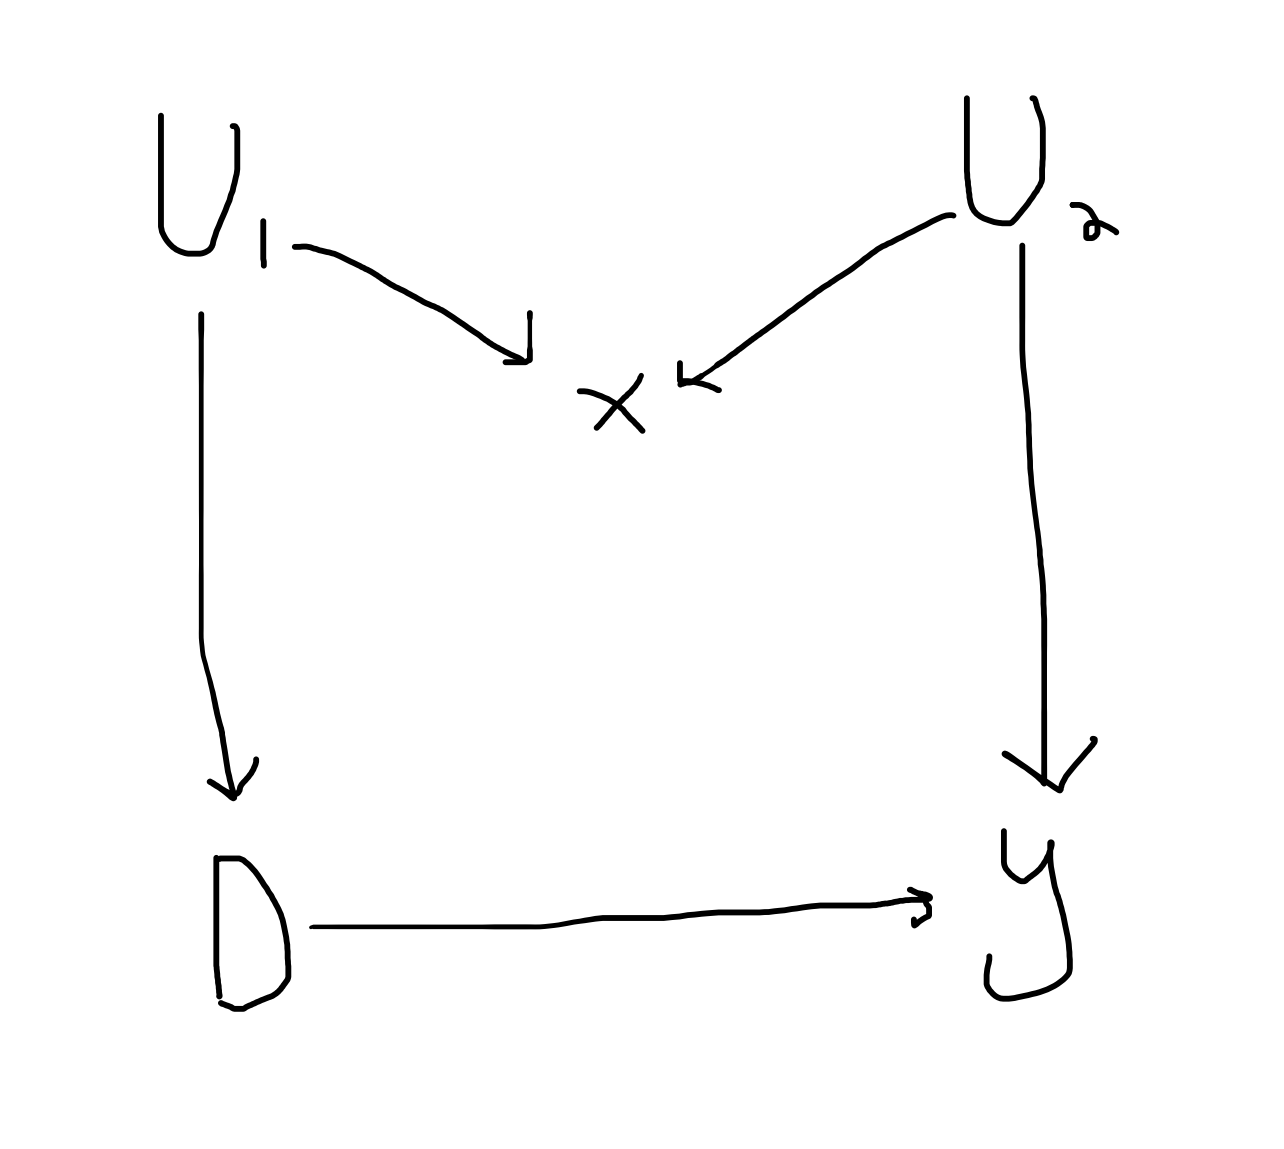
\includegraphics[scale=0.5,height=6.5cm, width=10cm]{./lecture_includes/mbias}

\footnotesize
$X$ is pre-treatment, but if you conditioned on it, then $D\leftarrow U1 \rightarrow \mbox{X} \leftarrow U2 \rightarrow Y$ and $X$ is a collider. Colliders take strange forms, so the conditioning set \emph{must} be thoughtfully chosen based on being a strong predictor of $Y^0$, preferably based on expert knowledge and not a kitchen sink of all available regressors

\end{frame}



\begin{frame}{Contrast this with ordinary practices}

\begin{itemize}
\item Person attempts to ``control for omitted variable bias'' by including as many ``controls'' as possible
\item Person does not even attempt to think about treatment assignment mechanism and therefore has no idea what variables are colliders, covariates or confounders
\item Big data approaches to covariate adjustment is \emph{very dangerous} -- colliders introduce bias and without a model, there is no way you know what those are
\end{itemize}

\end{frame}

\begin{frame}{Covariate selection without DAGs}

\begin{itemize}
\item Short of an outright DAG, then the thing to be thinking about is this:
	\begin{itemize}
	\item What set of covariates are highly predictive of $Y^0$?
	\item What set of covariates are highly predictive of $D$?
	\item Are these covariates distributed enough across both treatment and control?
	\end{itemize}
\item This is more of a hunch approach, but at least it's based on reasoning through the treatment assignment mechanism as opposed to ``kitchen sink regressions''
\end{itemize}

\end{frame}

\begin{frame}{Falsifications}

\begin{itemize}
\item Covariates should not be affected by the treatment, so examining them as falsifications can help establish the credibility of unconfoundedness
\item Falsification exercises are sometimes versions of this -- a gun control law shouldn't affect automobile theft or petty larceny
\item Imbens and Rubin (2015) suggested using the lagged outcome (pre-treatment) as a way of checking, as those have similar confounder structures
\item One study questioned a finding that obesity was contagious in social networks by estimating the same model on things that cannot be contagious like acne, headaches and height and found the same things (likely confounding existed)
\end{itemize}

\end{frame}


\begin{frame}[plain]

	\begin{block}{Identifying assumption I: Unconfoundedness}
	$(Y_i^0$, $Y_i^1)$ $\independent{D} | X_i$. There exists a set $X$ of known and quantified confounders such that after adjusting for them, treatment assignment is \emph{independent of potential outcomes}.
	\end{block}
	
	\begin{itemize}
	\item Conditional on $X$, treatment assignment is randomly distributed (i.e., independent of both potential outcomes) -- strong assumption
	\item For a large group of people within the same strata, they flipped coins as opposed to sought treatments that helped them
	\item Eliminating all backdoor paths on a DAG through blocking satisfies unconfoundedness; also called ignorability
	\end{itemize}
\end{frame}


\begin{frame}[plain]

	\begin{block}{Identifying assumption I: Unconfoundedness}
	$(Y_i^0$, $Y_i^1)$ $\independent{D} | X_i$. There exists a set $X$ of known and quantified confounders such that after adjusting for them, treatment assignment is \emph{independent of potential outcomes}.
	\end{block}
	
	\begin{eqnarray*}
	\alert{E[Y^0 | D=1, X=x]} &=& E[Y^0 | D=0, X=x] \\
	E[Y^1 | D=1, X=x] &=& \alert{E[Y^1 | D=0, X=x] }
	\end{eqnarray*}
	
Unconfoundedness justifies substituting units in treatment for control based on $X=x$ -- but only if there are exact matches (next slide)
	
	
\end{frame}



\begin{frame}[plain]

	\begin{block}{Identifying assumption II: Common support}
	For ranges of $X$, there is a positive probability of being both treated and untreated
	\end{block}
	
	\begin{itemize}
	\item There exists units in treatment and control with same values of $X$ -- you can't make the substitutions otherwise
	\item Dimension $k$ means every specific combination of the conditioning set (e.g., not males and old, but adult males, adult females, youth male, youth female)
	\item Testable because common support is observable unlike unconfoundedness, but as you can imagine if the dimensions of $X$ gets large (and with a continuous covariate it's infinite!) then it won't hold in any finite sample!
	\end{itemize}
	
	
\end{frame}



\begin{frame}{Assumptions combined}
	
But if we have them both (represented below), we can even outside of an RCT estimate the ATE through nonparametric matching
  \begin{enumerate}
		\item $(Y^1,Y^0) \independent{D} | X$ (strong unconfoundedness)
		\item $0<Pr(D=1|X)<1$ with probability one (common support)
  \end{enumerate}

\bigskip
Comparing groups of individuals \emph{who have the same values of} $X$, treatment is no longer based gains, $\delta$. 

\bigskip

The second term implies we have people in treatment and control for every strata of $X$
\end{frame}


\begin{frame}{Implications of assumptions}


	\begin{itemize}
	\item Assumption 1 lets you plug $Y$ for $Y^j$ with the switching equation
		\begin{eqnarray*}
		E[Y^1-Y^0|X] &=& E[Y^1 - Y^0 | X,D=1] \\
		&=&E[Y|X,D=1] - E[Y|X,D=0]
		\end{eqnarray*}
	\item Assumption 2 lets you weight over the covariate distribution
		\begin{eqnarray*}
		\delta_{ATE} &=&E[Y^1-Y^0] = E\bigg[ E[Y^1 - Y^0 \ \vert \ X] \bigg] \\
		&=& \int E[Y^1 - Y^0 |X,D=1] dPr(X) \\
		&=& \int \left(E[Y|X,D=1] - E[Y|X,D=0]\right)dPr(X)
		\end{eqnarray*}
	\end{itemize}

\end{frame}


\begin{frame}{Maybe You Want the ATT}


If we want the ATT, we can go with strictly weaker assumptions -- weak unconfoundedness and weak overlap

\bigskip

You can get a PhD because you care about your happiness with one $Y^1$; you just have to have acted independent of what you gave up $Y^0$

\end{frame}




\begin{frame}{ATT Identification}

We can modify those assumptions and weaken both which helps a lot

\begin{enumerate}
  \item $Y^0 \independent{D} | X$ (weak unconfoundedness)
  \item $Pr(D=1|X)<1$ (with $Pr(D=1)>0$) (weak support)
\end{enumerate}

\bigskip

We don't need full common support because we don't need to find counterfactuals for the control group -- we only need units in the control group that match with our treatment group

\bigskip

Selection is weaker too, like I said -- they are not entirely irrational, but who knows if it helps you

\end{frame}



\begin{frame}{Summarizing}


Weighted averages under both assumptions:
		\begin{eqnarray*}
		\delta_{ATT} &=& \int \left(E[Y|X,D=1] - E[Y|X,D=0]\right)dPr(X|D=1)
		\end{eqnarray*}
We match units in treatment and control because under weak unconfoundedness they're substitutable, and we use weak common support so that we can actually do it, then we take weighted averages over the differences.  
		
\end{frame}



\subsection{Exact and Inexact Matching}

\begin{frame}{Exact matching}

\begin{figure}[!t]\centering
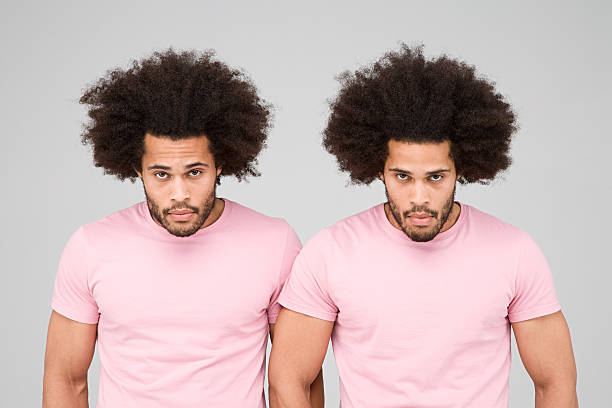
\includegraphics[scale=1.1]{./lecture_includes/identical_twins}
\end{figure}

\end{frame}

\begin{frame}{Quote from Imbens and Rubin 2015}

\begin{quote}
``At some level, all methods for causal inference can be viewed as imputation methods, although some more explicitly than others.''
\end{quote}

\bigskip

Matching goes back at least to Rubin's early work on the propensity score, but we will start with nearest neighbor matching as there's ideas there we draw upon later with synth I want to emphasize

\bigskip

Matching will match a treated unit to a comparison unit that is similar (or in exact matching identical) on a known and quantified confounder



\end{frame}



\begin{frame}{Training example (unmatched)}

{\renewcommand{\arraystretch}{1.1}
\tabcolsep=2.5\tabcolsep
\begin{table}[htb]\tiny\index{rolling!3}
\centering
\begin{tabular}{ccc|ccc}
\toprule
	\multicolumn{3}{c}{\textbf{Trainees}}&
	\multicolumn{3}{c}{\textbf{Non-Trainees}}\\
	\multicolumn{1}{c}{Unit}&
	\multicolumn{1}{c}{Age}&
	\multicolumn{1}{c}{Earnings}&
	\multicolumn{1}{c}{Unit}&
	\multicolumn{1}{c}{Age}&
	\multicolumn{1}{c}{Earnings}\\
\midrule
1 & 	31 & \$	26,629 & 	1 & 	29 & \$	23,178 \\
2 & 	31 & \$	26,633 & 	2 & 	39 &\$ 	33,817 \\
3 & 	18 & 	\$	15,324 & 	3 & 	33 & \$	27,061 \\
4 & 	32 &\$ 	27,717 & 	4 & 	46 & \$	43,109 \\
5 & 	32 & \$	27,725 & 	5 & 	32 & \$	26,040 \\
6 & 	25 & \$	20,762 & 	6 & 	39 & \$	33,815 \\
7 & 	32 &\$ 	27,716 & 	7 & 	31 & \$	25,052 \\
8 & 	32 & \$	27,719 & 	8 & 	33 & \$	27,060 \\
9 & 	20 & \$	16,723 & 	9 & 	25 &\$ 	19,787 \\
10 & 	29 & \$	24,552 & 	10 & 	29 &\$ 	23,173 \\
&&&			11 & 	27 & 	21,416 \\
&&&			12 & 	32 & 	26,040 \\
&&&			13 & 	20 & 	16,246 \\
&&&			14 & 	41 & 	36,316 \\
&&&			15 & 	18 & 	15,046 \\
&&&			16 & 	29 & 	23,178 \\
&&&			17 & 	49 & 	47,559 \\
&&&			18 & 	32 & 	26,040 \\
&&&			19 & 	27 & 	21,418 \\
&&&			20 & 	46 & 	43,109 \\
\midrule
Mean & 	28.2 & 	\$24,150 & 	Mean & 	32.85 & 	\$27,923 \\
\bottomrule
\end{tabular}
$SDO = \$24,150-27,923 = -\$3,773$
\end{table}
}


\end{frame}


\begin{frame}{Age Imbalance}

\begin{figure}[!t]\centering
\caption{Age distribution of a job training program's trainees (figure a) versus a sample of workers who were not enrolled in the trainee program (figure b).}
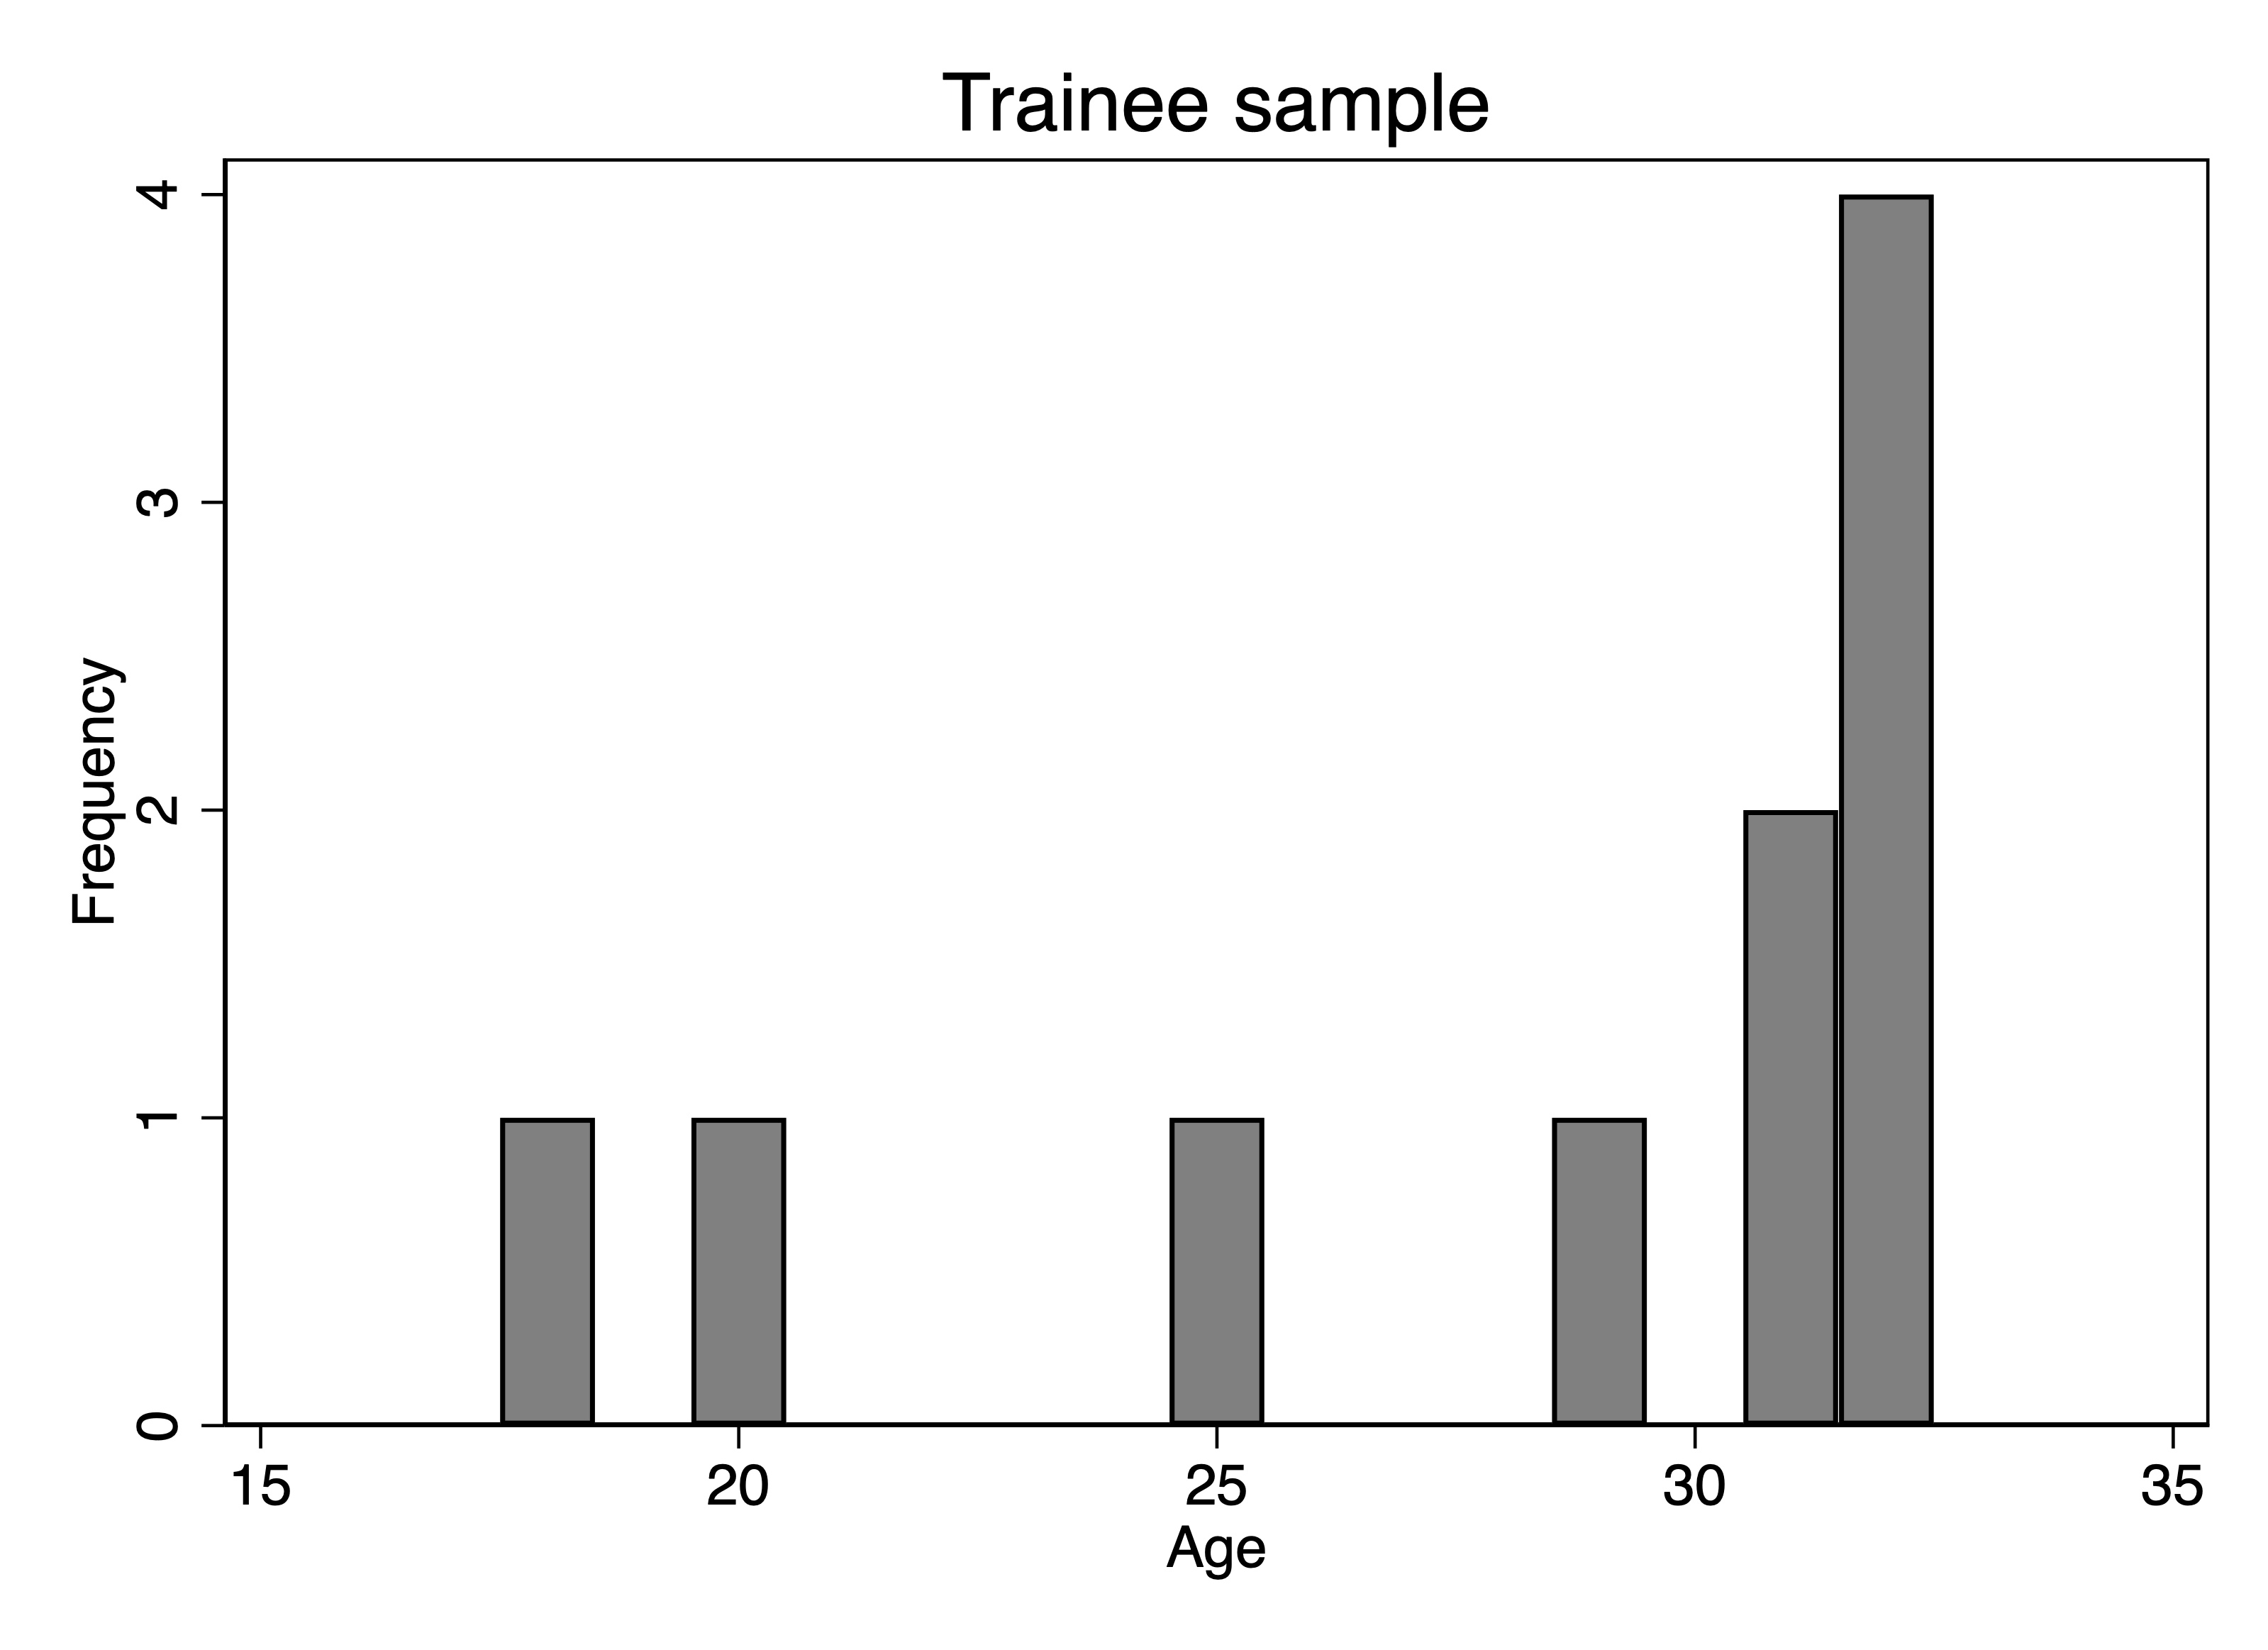
\includegraphics[scale=0.075]{./lecture_includes/trainees.jpg}
\end{figure}

\end{frame}

\begin{frame}{Age Imbalance}

\begin{figure}[!t]\centering
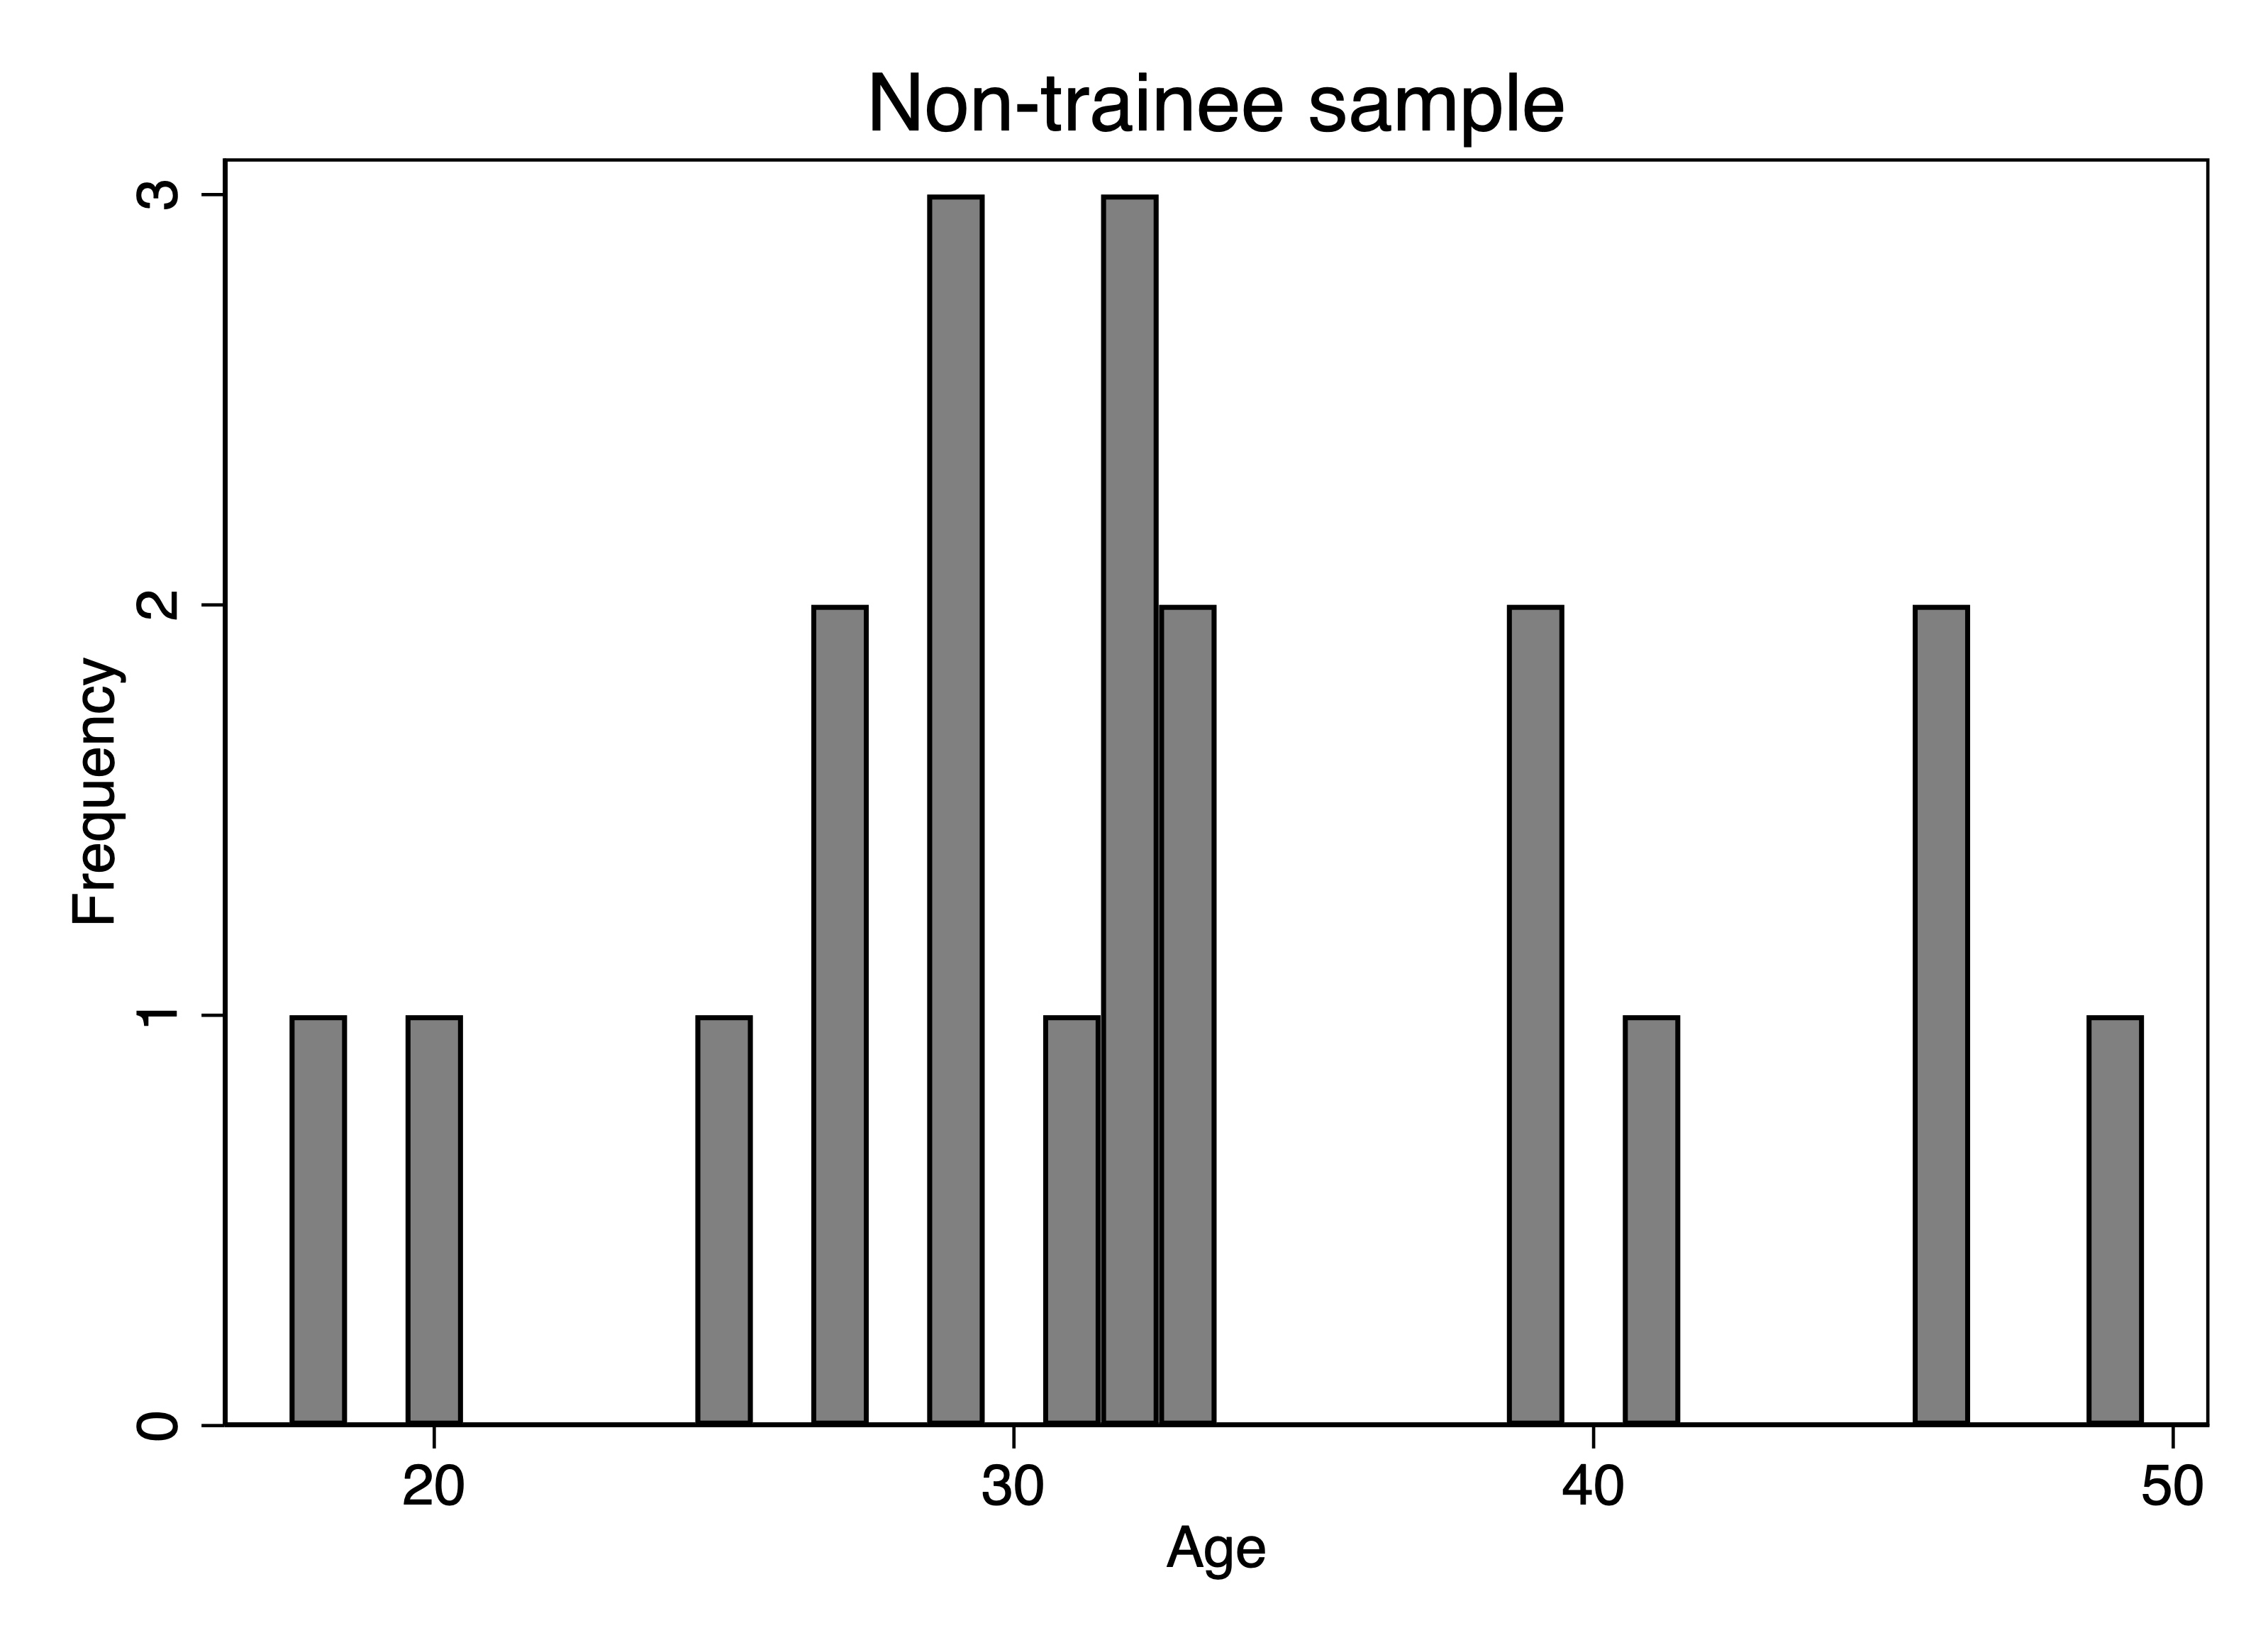
\includegraphics[scale=0.075]{./lecture_includes/nontrainees}
\end{figure}

\end{frame}

\begin{frame}{Exact matching}

\begin{itemize}
\item Exact matching finds a person in the control group whose value of $X_j$ is \emph{exactly} equal to each person in the treatment group $i$
\item Will not work if the conditioning set includes a continuous variable
\item Will also not work if $K$ gets large (curse of dimensionality we discuss later)
\end{itemize}

\end{frame}



\begin{frame}{ATT estimator}

We will focus on the ATT for the rest of today and the equation is:

\begin{equation}
\widehat{\delta}_{ATT} = \dfrac{1}{N_T} \sum_{D_i=1}(Y_i - Y_{j(i)})
\label{eq:att_simplematch}
\end{equation}

where $Y_{j(i)}$ is the $j$\textsuperscript{th} unit matched to the $i$\textsuperscript{th} unit based on the $j$\textsuperscript{th} being ``exactly equal to'' the $i$\textsuperscript{th} unit with respect to the $X$ conditioning set

\end{frame}

\begin{frame}{Number of matches}

What if I find two or more $M$ units with the identical $X$ value? Then what?

\begin{equation}
\widehat{\delta}_{ATT} = \dfrac{1}{N_T} \sum_{D_i=1} \bigg ( Y_i - \bigg [\dfrac{1}{M} \sum_{m=1}^M Y_{j_m(1)} \bigg ] \bigg )
\label{eq:att_match}
\end{equation}

\bigskip

Notice that we are only dealing with $Y^0_i$ by matching; The $Y^1_i$ is fine as is.

\end{frame}

\begin{frame}{Matching algorithm}

\begin{enumerate}
\item For each unit $i$ in the treatment group with known and quantified confounder $X=x_i$, find all units $j$ in the donor pool for whom $x_i=x_j$. These $j$ units are our $M$ matches and $M$ can be one or it can be greater than one if you want it to be.
\item For each unit $i$, replace its missing potential outcome, $Y^0_i$, with the matched $j$ units' realized outcomes, $\frac{1}{M} \sum {Y}_{j(i)}$, from Step 1. Do this for all $i$ units in the treatment group.
\item For each unit $i$, calculate the difference between realized earnings and matched earnings, $\widehat{\delta}_i=Y_i - \frac{1}{M} \sum {Y}_{j(i)}$.
\item Finally, estimate the sample ATT by averaging over all $i$ differences in earnings from Step 3 as $\frac{1}{N_T} \sum \widehat{\delta}_i$, where $N_T$ is the number of treatment units.
\end{enumerate}

\end{frame}



\begin{frame}{Matched sample}

\begin{table}[htb]\small\index{rolling!3}
\caption{Training example with matched sample using exact matching}
\centering
\begin{tabular}{ccc|ccc}
\toprule
	\multicolumn{3}{c}{\textbf{Trainees}}&
	\multicolumn{3}{c}{\textbf{Matched Sample}}\\
	\multicolumn{1}{c}{Unit}&
	\multicolumn{1}{c}{Age}&
	\multicolumn{1}{c}{Earnings}&
	\multicolumn{1}{c}{Matched Unit}&
	\multicolumn{1}{c}{Age}&
	\multicolumn{1}{c}{Earnings}\\
\midrule
1&	31&	\$26,693&	2&	31&	\$25,052 \\
2&	31&	\$26,691&	2&	31&	\$25,052 \\
3&	18&	\$15,392&	18&	18&	\$15,046 \\
4&	32&	\$27,776&	5&	32&	\$26,045 \\
5&	32&	\$27,779&	5&	32&	\$26,045 \\
6&	25&	\$20,821&	4&	25&	\$19,787 \\
7&	32&	\$27,778&	5&	32&	\$26,045 \\
8&	32&	\$27,780&	5&	32&	\$26,045 \\
9&	20&	\$16,781&	8&	20&	\$16,246 \\
10&	29&	\$24,610&	6&	29&	\$23,178 \\
\midrule
Mean&	28.2&	\$24,210&	Mean&	28.2&	\$22,854 \\
\bottomrule
\end{tabular}
\end{table}
\footnotesize
$\widehat{ATT} = \$24,210 - \$22,854 = \$1,356$


\end{frame}

\begin{frame}{Estimated ATT using Exact Matching}


Weak unconfoundedness of $Y^0$ with respect to age justified substituting one group for another

\bigskip

But matching bias still exists if you fail common support -- unconfoundedness is necessary but not sufficient

\bigskip

Even weak support is rare due to the curse of dimensionality

\end{frame}





\begin{frame}{Inexact matching}

\begin{figure}[!t]\centering

\includegraphics[scale=0.75]{./lecture_includes/fraternal_twins}
\end{figure}

\end{frame}


\begin{frame}{Curse of Dimensionality}
	
	\begin{itemize}
	\item If no matches can be found, it means many cells may contain either only treatment units or only control units but not both, and that violates our common support assumption
	\item We can always use ``finer'' classifications, but finer cells worsens the dimensional problem, so we don't gain  much from that.  ex: using $10$ variables and $5$ categories for each, we get $5^{10} = 9,765,625$.  
	\item Matching methods really force us to see these curses; they're often hidden from OLS because OLS uses extrapolations based off functional form
	\end{itemize}
\end{frame}	


\begin{frame}{Propensity scores}

\begin{itemize}
\item Propensity scores were developed by Rosenbaum and Rubin (1983) as a way of reducing the dimension of the conditioning set of $X$
\item But it still requires common support -- propensity scores don't solve the curse of dimensionality problem from the perspective of bias
\item If you don't have exact matches in the dimensions of $X$ then you'll still be matching units with similar propensity scores but it won't overcome the bias
\item There are methods that will adjust the propensity score estimation which I'll briefly mention at the end

\end{itemize}

\end{frame}




\begin{frame}{To Look Like Someone Else}

\begin{itemize}
\item When we can make synthetic xerox copies of ourselves, that's exact matching
\item But what if we can only make similar copies of ourselves, like fraternal, but not identical, twins? That's nearest neighbor matching -- a form of ``inexact matching'', sort of like fraternal twins
\item Introduces bias bc of inexact matching, but the magnitude of the bias depends on the severity of the discrepancy
\item We can improve on nearest neighbor matching using bias adjustment (Abadie and Imbens 2011) 
\end{itemize}

\end{frame}

\begin{frame}{Nearest Neighbor Matching}
	
	\begin{itemize}
	\item Estimate $\widehat{\delta}_{ATT}$ by \emph{imputing} the missing potential outcome of each treatment unit $i$ using the observed outcome from that outcome's ``nearest'' neighbor $j$ in the control set using $X$ for the matching
		\begin{eqnarray*}
		\widehat{\delta}_{ATT} = \frac{1}{N_T}\sum_{D_i=1} (Y_i - Y_{j(i)})
		\end{eqnarray*}where $Y_{j(i)}$ is the observed outcome of a control unit such that $X_{j(i)}$ is the \textbf{closest} value to $X_i$ among all of the control observations (eg match on $X$)
	\end{itemize}
\end{frame}

\begin{frame}{Matching}
	
	\begin{itemize}
	\item We could also use the average observed outcome over $M$ closest matches:
		\begin{eqnarray*}
		\widehat{\delta}_{ATT} = \frac{1}{N_T}\sum_{D_i=1}\left(Y_i-\left[\frac{1}{M}\sum_{m=1}^MY_{j_m(1)}\right]\right)
		\end{eqnarray*}
	\item Works well when we can find good matches for each treatment group unit, so $M$ is usually defined to be small (i.e., $M=1$ or $M=2$)
	\end{itemize}
\end{frame}



\begin{frame}{Matching example with single covariate}
	
	\begin{table}
	\begin{tabular}{c|c|c|c|c}
	\hline
	$i$ & $Y^1_i$ & $Y^0_i$ & $D_i$ & $X_i$ \\
	\hline
	1 & 6 &  \textcolor{red}{?} & 1 & 3 \\
	2 & 1 &  \textcolor{red}{?} & 1 & 1 \\
	3 & 0 &   \textcolor{red}{?} & 1 & 10 \\
	\hline
	4 &  & 0 & 0 & 2 \\
	5 &  & 9 & 0 & 3 \\
	6 &  & 1 & 0 & -2 \\
	7 &  & 1 & 0 & -4 \\
	\hline
	\end{tabular}
	\end{table}
	
	
	\begin{flalign*}
		    \only<1-2>{&\text{Question: What is }\widehat{\delta}_{ATT}=\frac{1}{N_T} \sum_{D_i=1} (Y_i - Y_{j(i)})\text{?}}& \\
		    \only<2-2>{&\text{Match and plug in!}} \\
 	\end{flalign*}

\end{frame}
	
	
\begin{frame}{Matching example with single covariate}
	
	\begin{table}
	\begin{tabular}{c|c|c|c|c}
	\hline
	$i$ & $Y^1_i$ & $Y^0_i$ & $D_I$ & $X_i$ \\
	\hline
	1 & 6 &  \textcolor{blue}{9} & 1 & \textcolor{blue}{3} \\
	2 & 1 &  \textcolor{green}{0} & 1 & \textcolor{green}{1} \\
	3 & 0 &   \textcolor{blue}{9} & 1 & \textcolor{blue}{10} \\
	\hline
	4 &  & \textcolor{green}{0} & 0 & \textcolor{green}{2} \\
	5 &  & \textcolor{blue}{9} & 0 & \textcolor{blue}{3} \\
	6 &  & 1 & 0 & -2 \\
	7 &  & 1 & 0 & -4 \\
	\hline
	\end{tabular}
	\end{table}
	
	
	\begin{flalign*}
		&\text{Question: What is }\widehat{\delta_{ATT}}=\frac{1}{N_T} \sum_{D_i=1} (Y_i - Y_{j(i)})\text{?}& \\
		&\widehat{\delta}_{ATT} = \frac{1}{3} \cdot (6-\textcolor{blue}{9}) + \frac{1}{3} \cdot (1-\textcolor{green}{0}) + \frac{1}{3} \cdot (0-\textcolor{blue}{9}) = -3.7
	\end{flalign*}

\end{frame}


%{
%\setbeamercolor{background canvas}{bg=}
%\includepdf[pages=1-last]{./lecture_includes/abadie-matching2.pdf}
%}



\begin{frame}{Measuring the matching discrepancy}

\begin{itemize}
\item What does it mean to be close when I am working with a large number of covariates?
\item What if we had a way of measuring a match in terms of how ``close'' each unit's $X_i$ value was to the matched $X_j$
\item Let's do that and use the square root of the sum of all squared differences in each unit's $X_i - X_{j(i)}$ as a measure of how bad the match is
\item This is called the Euclidean distance
\end{itemize}


\end{frame}

%\begin{frame}{Alternative distance metric: Euclidean distance}
	
% When the vector of matching covariates, $X= \colvec{X_1\\X_2\\\vdots\\X_k}$ has more than one dimension ($k>1$) we will need a new definition of \textbf{distance} to measure ``closeness''.  
%\end{frame}

\begin{frame}{Euclidean distance}
	\begin{block}{Definition: Euclidean distance}
    \vspace*{-2.5mm}
    \begin{eqnarray*}
    ||X_i-X_j|| &=& \sqrt{ (X_i-X_j)'(X_i-X_j) } \\
    &=& \sqrt{ \sum_{n=1}^k (X_{ni} - X_{nj})^2 }
    \end{eqnarray*}
    \vspace*{-2.5mm}
	\end{block}
	
Let's do this together -- sometimes it helps to manually calculate this

\bigskip

\url{https://docs.google.com/spreadsheets/d/1iro1Qzrr1eLDY_LJVzOYvnQZWmxY8JyTcDf6YcdhkwQ/edit?usp=sharing}

	
\end{frame}


\begin{frame}{Inexact matching: Random match 1}

\begin{figure}[!t]\centering
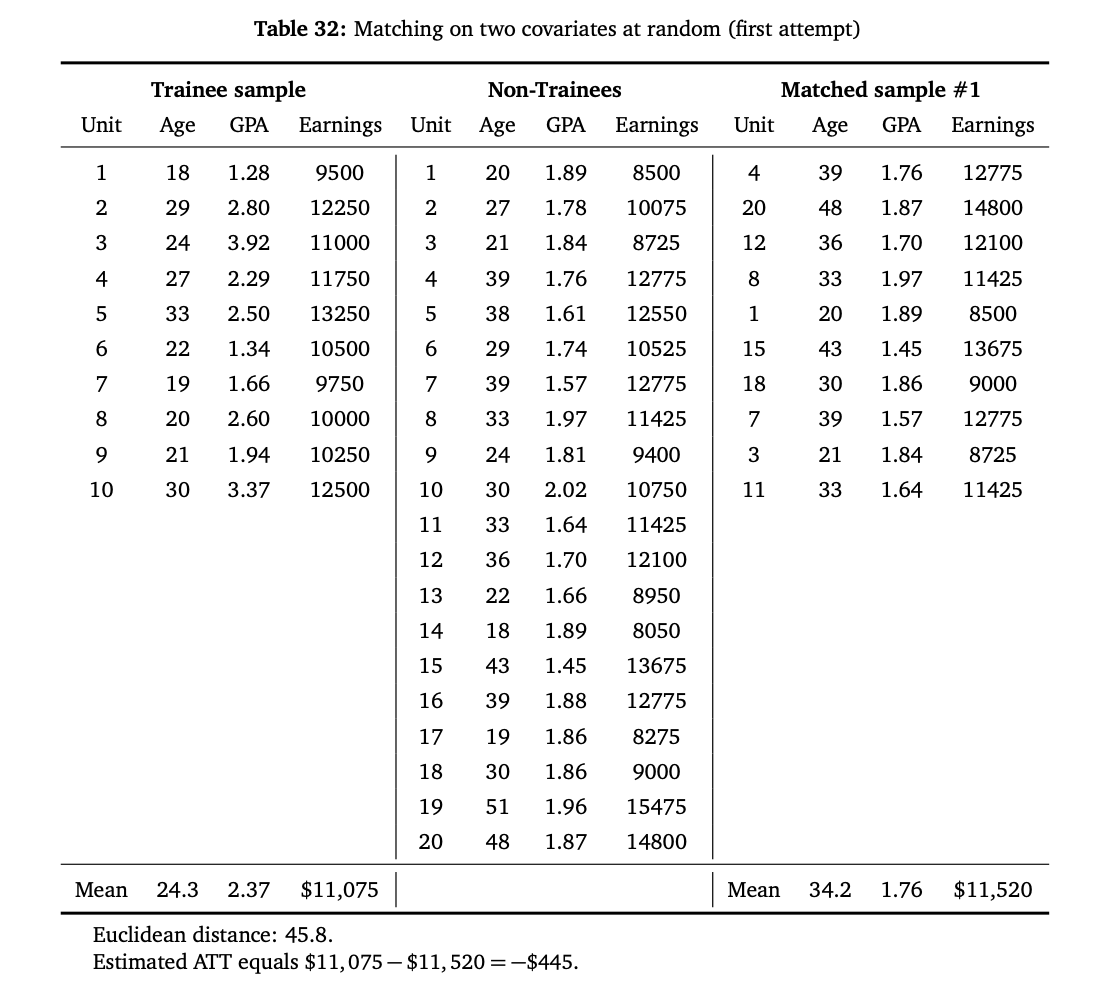
\includegraphics[scale=0.45]{./lecture_includes/inexact_random1}
\end{figure}

\end{frame}


\begin{frame}{Inexact matching: Random match 2}

\begin{figure}[!t]\centering
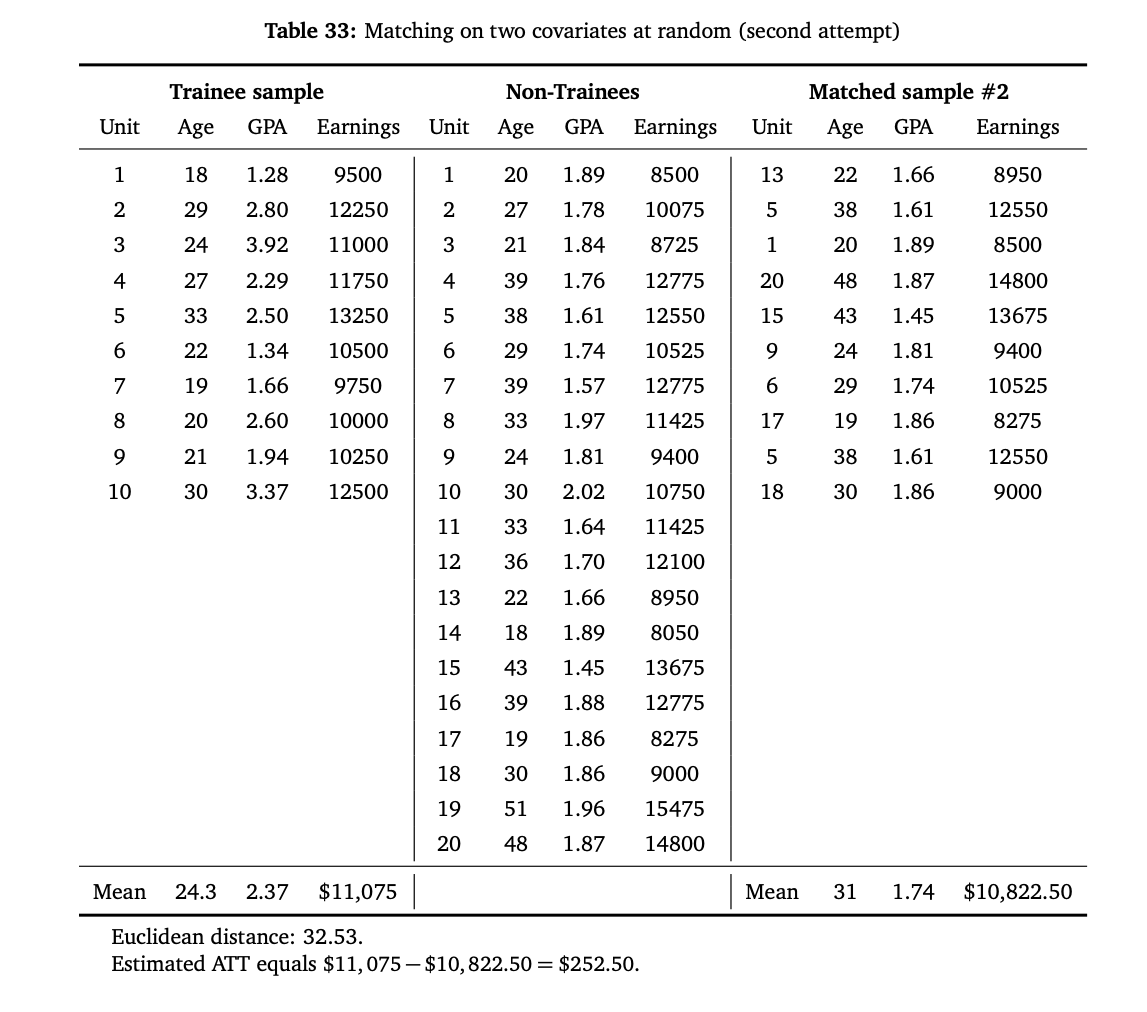
\includegraphics[scale=0.45]{./lecture_includes/inexact_random2}
\end{figure}

\end{frame}


\begin{frame}{Minimizing the Euclidean distance}

\begin{itemize}
\item Abadie and Imbens (2006) show that there exists a unique solution to the matching problem that minimizes a given distance metric 
\item \texttt{Matching} in R and \texttt{teffects} in Stata (not sure in python)
\item But the idea here is that any other match will always have a higher Euclidean distance so I've drawn a picture!
\end{itemize}

\end{frame}


\begin{frame}{Visualization of Optimal Match}

\begin{figure}[!t]\centering
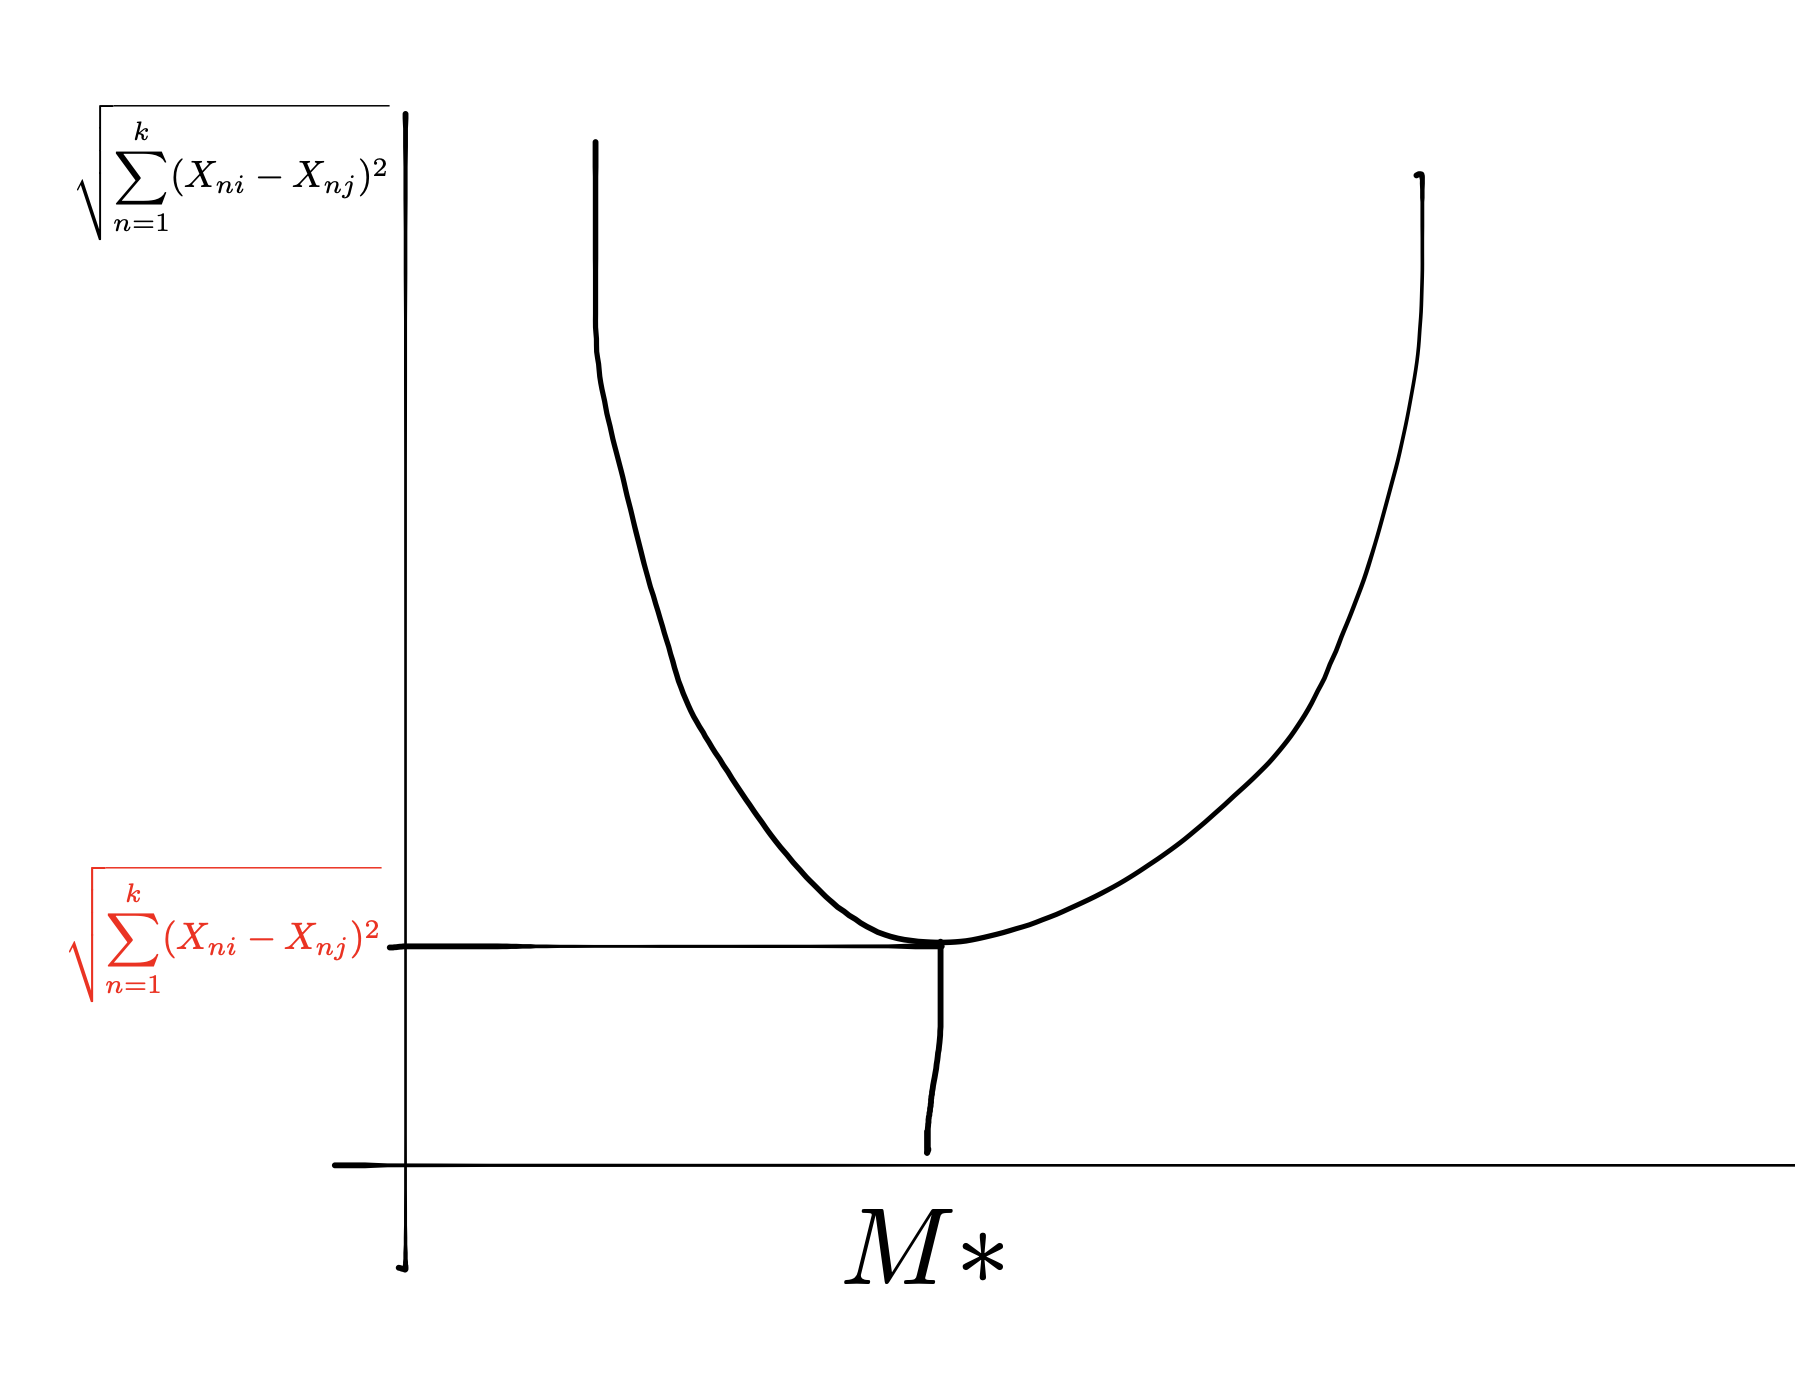
\includegraphics[scale=0.35]{./lecture_includes/optimal_matches}
\end{figure}

\end{frame}




\begin{frame}{Inexact matching by minimizing the Euclidean distance}

\begin{figure}[!t]\centering
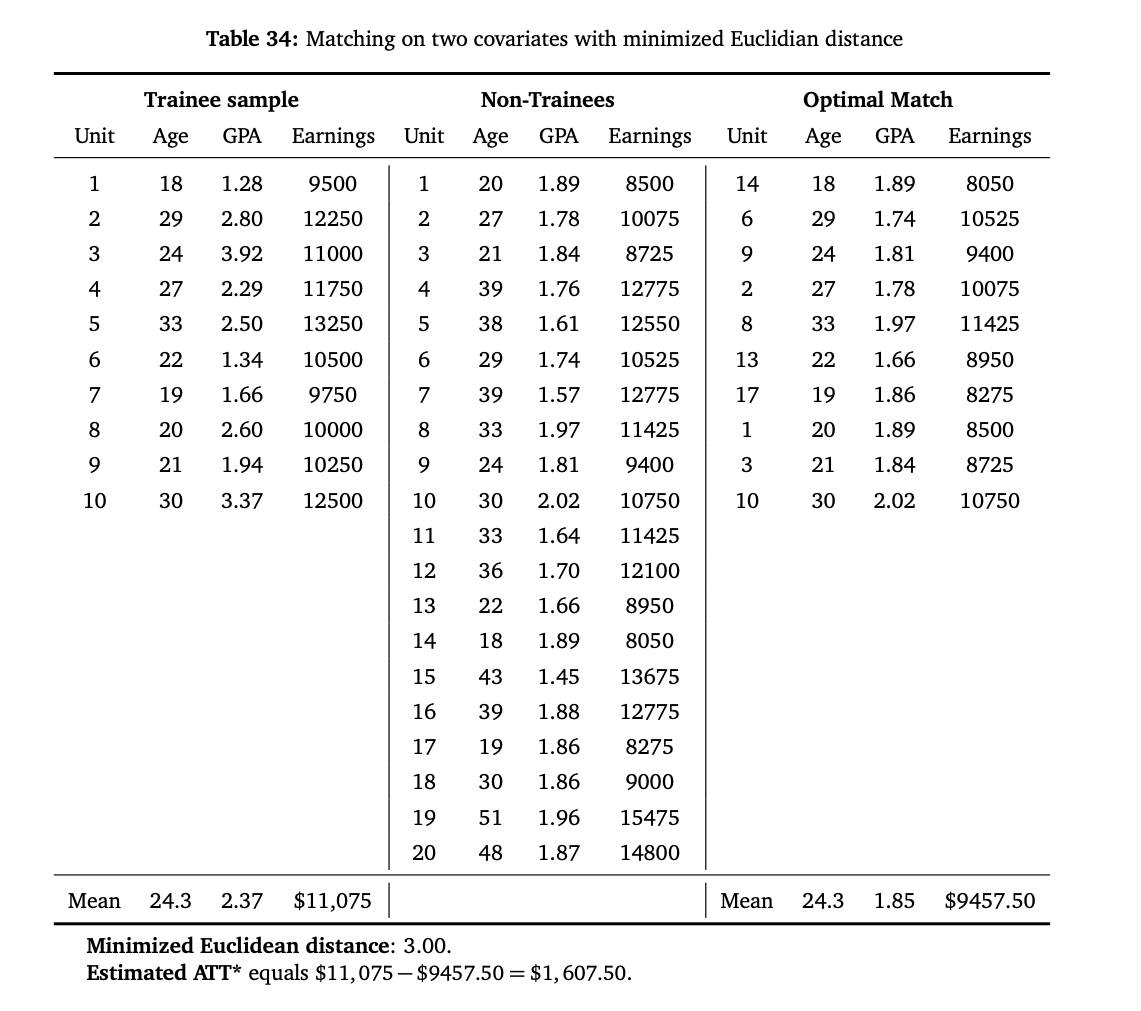
\includegraphics[scale=0.45]{./lecture_includes/inexact_euclidean}
\end{figure}

\end{frame}

\begin{frame}{Other distance metrics}

\begin{itemize}
\item Our example treated a one unit difference in age and one unit difference in GPA as the same, but those scales are different and matter a lot
\item The Euclidean distance is not invariant to changes in the scale of the $X$'s.  
\item Alternative distance metrics that \emph{are} invariant to changes in scale are more commonly used 
\item Normalized Euclidean distance and Mahalanobis distance both try to normalize it so that scale doesn't matter
\end{itemize}

\end{frame}


\begin{frame}{Normalized Euclidean distance}

	\begin{block}{Definition: Normalized Euclidean distance}
	  A commonly used distance is the normalized Euclidean distance:$$||X_i-X_j|| = \sqrt{ (X_i-X_j)'\widehat{V}^{-1}(X_i - X_j) }$$ where
		$$\widehat{V}^{-1} = \text{diag}(\widehat{\sigma}_1^2, \widehat{\sigma}_2^2, \dots, \widehat{\sigma}_k^2)$$
	\end{block}
\end{frame}

\begin{frame}{Normalized Euclidean distance}
	\begin{itemize}
	\item Notice that the normalized Euclidean distance is equal to:
		\begin{eqnarray*}
		||X_i - X_j|| = \sqrt{\sum_{n=1}^k \frac{(X_{ni} - X_{nj})^2}{\widehat{\sigma}^2_n}}
		\end{eqnarray*}
	\item Thus, if there are changes in the scale of $X_{ni}$, these changes also affect $\widehat{\sigma}^2_n$, and the normalized Euclidean distance does not change
	\end{itemize}

\end{frame}


\begin{frame}{Mahalanobis distance}
	
	\begin{block}{Definition: Mahalanobis distance}
	The Mahalanobis distance is the scale-invariant distance metric:
		\begin{eqnarray*}
		||X_i-X_j|| = \sqrt{ (X_i-X_j)'\widehat{\Sigma}_X^{-1}(X_i - X_j) }
		\end{eqnarray*}
	where $\widehat{\Sigma}_X$ is the sample variance-covariance matrix of $X$.
	\end{block}


\end{frame}



\begin{frame}{Matching and the Curse of Dimensionality}
	
\begin{itemize}
\item The larger the dimensions of the conditioning set, the less likely common support holds, and you can't not do it because you need these covariate dimensions to satisfy weak unconfoundedness!
\item This problem is caused by the finite dataset, and it introduces a particular type of selection bias
\item Curses are only overcome with new spells  
\item Abadie and Imbens (2011) derived a way to reduce the bias (bias adjustment or bias correction)
\end{itemize}

\end{frame}


\begin{frame}{Deriving the matching bias}
	
  \vspace{-5mm}
  $$
		\widehat{\delta}_{ATT} = \frac{1}{N_T} \sum_{D_i=1} (Y_i - Y_{j(i)}),
  $$
  where each $i$ and $j(i)$ units are matched, $X_i \approx X_{j(i)}$ and $D_{j(i)}=0$. 
	 
  \bigskip
  Define potential outcomes and switching eq.
		\begin{eqnarray*}
      \mu^0(x) &=& E[Y | X=x,D=0] = E[Y^0 | X=x],\\
      \mu^1(x) &=& E[Y | X=x,D=1] = E[Y^1 | X=x],\\
      Y_i &=& \mu^{D_i}(X_i) + \varepsilon_i
		\end{eqnarray*}
\end{frame}

\begin{frame}{Deriving the matching bias}
  Substitute and distribute terms
  \begin{eqnarray*}
    \widehat{\delta}_{ATT} &=& \frac{1}{N_T} \sum_{D_i=1} (Y_i - Y_{j(i)}) \\
    &=& \frac{1}{N_T} \sum_{D_i=1} \left[ (\mu^1(X_i) + \varepsilon_i) - (\mu^0(X_{j(i)}) + \varepsilon_{j(i)}) \right] \\
    &=&  \frac{1}{N_T} \sum_{D_i=1} (\mu^1(X_i) - \mu^0(X_{j(i)})) + \frac{1}{N_T} \sum_{D_i=1}(\varepsilon_i - \varepsilon_{j(i)})
  \end{eqnarray*}
\end{frame}
		

\begin{frame}{Deriving the matching bias}
	
Difference between sample estimate and population parameter is:
		\begin{eqnarray*}
		\widehat{\delta}_{ATT} - \delta_{ATT} &=& \frac{1}{N_T} \sum_{D_i=1} \left( \mu^1(X_i) - \mu^0(X_{j(i)}) - \delta_{ATT}\right) \\
		&+& \frac{1}{N_T} \sum_{D_i=1} (\varepsilon_i - \varepsilon_{j(i)})
		\end{eqnarray*}
Algebraic manipulation and simplification:
		\begin{eqnarray*}
		\widehat{\delta}_{ATT} - \delta_{ATT} &=& \frac{1}{N_T} \sum_{D_i=1} \left( \mu^1(X_i) - \mu^0(X_i) - \delta_{ATT}\right) \\
		&+& \frac{1}{N_T} \sum_{D_i=1} (\varepsilon_i - \varepsilon_{j(i)}) \\
		&+& \frac{1}{N_T} \sum_{D_i=1} \left( \mu^0(X_i) - \mu^0(X_{j(i)}) \right).
		\end{eqnarray*}
\end{frame}


\begin{frame}{Deriving the matching bias}
	
Note $\widehat{\delta}_{ATT} - \delta_{ATT} \to 0$ as $N \to \infty$.
\pause However, 
$$E[ \sqrt{\frac{1}{N}} (\widehat{\delta}_{ATT} - \delta_{ATT})] = E[ \sqrt{\frac{1}{N}} ( \mu^0(X_i) - \mu^0(X_{j(i)}) ) | D=1].$$ 
\pause
Now consider the implications if $k$ is large:
\pause	\begin{itemize}
	\item The difference between $X_i$ and $X_{j(i)}$ converges to zero very slowly 
\pause	\item The difference $\mu^0(X_i) - \mu^0(X_{j(i)})$ converges to zero very slowly \pause
	\item $E[ \sqrt{\frac{1}{N}} (\mu^0(X_i) - \mu^0(X_{j(i)})) | D=1]$ may not converge to zero and an be very large! 
\pause	\item $E[ \sqrt{\frac{1}{N}} (\widehat{\delta}_{ATT} - \delta_{ATT})]$ may not converge to zero because the bias of the matching discrepancy is dominating the matching estimator! \pause
	\end{itemize}
 Bias is often an issue when we match in many dimensions
\end{frame}

\begin{frame}{Solutions to matching bias problem}
	
The bias of the matching estimator is caused by large matching discrepancies $||X_i - X_{j(i)}||$ which is virtually guaranteed by the curse of dimensionality.  However:
	\begin{enumerate}
	\item But the matching discrepancies are observed. We can always check in the data how well we're matching the covariates.

	\item For $\widehat{\delta}_{ATT}$ we can sometimes make the matching discrepancies small by using a large reservoir of untreated units to select the matches (that is, by making $N_C$ large).

  \item If the matching discrepancies are large, so we are worried about potential biases, we can apply bias correction techniques

	\end{enumerate}
\end{frame}


\begin{frame}{Matching with bias correction}
	
	\begin{itemize}
	\item Each treated observation contributes$$\alert{\mu^0(X_i)} - \mu^0(X_{j(i)})$$to the bias.
	\item Bias-corrected (BC) matching:
		\begin{eqnarray*}
		\widehat{\delta}_{ATT}^{BC} = \frac{1}{N_T} \sum_{D_i=1} \left[ (Y_i - Y_{j(i)}) - ( \widehat{\mu^0}(X_i) - \widehat{\mu^0}(X_{j(i)}) ) \right]
		\end{eqnarray*}where $\widehat{\mu^0}(X)$ is an estimate of $E[Y|X=x,D=0]$.  For example using OLS but other maybe too (neural nets?).  
	\item Under some conditions, the bias correction eliminates the bias of the matching estimator without affecting the estimator's variance.
	\end{itemize}
\end{frame}


\begin{frame}{Steps}

\begin{enumerate}
\item[1.  ]Regress $Y$ on $X$ with OLS except only use the control sample:
\begin{equation}
Y_j = \alpha + \beta X_j + \varepsilon_j \nonumber
\end{equation}where $j$ are the units for which $D_j=0$.  
\end{enumerate}

\end{frame}

\begin{frame}{Steps}

\begin{enumerate}
\item[2. ] Use the fitted values $\widehat{\alpha}$ and $\widehat{\beta}$ to predict $\widehat{\mu}^0(X)$ for both the $i$ and the matched $j(i)$ units:
\begin{eqnarray}
\widehat{\mu}^0_i &=& \widehat{\alpha} + \widehat{\beta} X_i \nonumber \\
\widehat{\mu}^0_{j(i)} &=& \widehat{\alpha} + \widehat{\beta} X_{j(i)} \nonumber
\end{eqnarray}
\end{enumerate}

\end{frame}


\begin{frame}{Steps}

\begin{enumerate}
\item[3. ] Subtract $ \widehat{\mu}_i^0(X_i) - \widehat{\mu}_{j(i)}^0(X_{j(i)})$, our estimate of the selection bias caused by matching discrepancies, from the sample estimate of the $ATT$: $$\widehat{\delta}_{ATT}^{BC} = \dfrac{1}{N_T} \sum_{D_i=1} \bigg [ (Y_i - Y_{j(i)}) - \Big(\widehat{\mu}^0(X_i) - \widehat{\mu}^0(X_{j(i)})\Big) \bigg ]$$
\end{enumerate}

\end{frame}


\begin{frame}{Steps}

\begin{enumerate}
\item[4. ] Estimate Abadie-Imbens robust standard error (Abadie and Imbens 2006; 2008; 2011)
\end{enumerate}

\end{frame}



\begin{frame}[plain,shrink=0]
	\begin{center}
	\textbf{Bias adjustment in matched data}
	\end{center}
	
	\begin{table}
	\begin{tabular}{c|c|c|c|c}
	\hline
	\multicolumn{1}{c}{}&
	\multicolumn{2}{c}{Potential Outcome}&
	\multicolumn{1}{c}{}&
	\multicolumn{1}{c}{}\\
	\multicolumn{1}{c}{unit} &
	\multicolumn{1}{c}{under Treatment}&
	\multicolumn{1}{c}{under Control}&
	\multicolumn{1}{c}{}&
	\multicolumn{1}{c}{}\\
	\hline
	$i$ & $Y^1_i$ & $Y^0_i$ & $D_i$ & $X_i$ \\
	\hline
	1 & \textcolor{blue}{10} &  \textcolor{blue}{8} & 1 & \textcolor{blue}{3} \\
	2 & 4 &  			 1 &				 1 & 1 \\
	3 & \textcolor{green}{10} &   \textcolor{green}{9} & 1 & \textcolor{green}{10} \\
	\hline
	4 &  & \textcolor{blue}{8} & 0 & \textcolor{green}{4} \\
	5 &  & 			 1 & 0 &  				0 \\
	6 &  & \textcolor{green}{9} & 0 & \textcolor{green}{8} \\
	\hline
	\end{tabular}
	\end{table}
	
	
	\begin{flalign*}
		\only<1-3>{&\widehat{\delta}_{ATT} = \frac{10-8}{3} + \frac{4-1}{3}  + \frac{10-9}{3}  = 2&} \\
		\only<2-3>{&\text{For the bias correction, estimate }\widehat{\mu^0}(X) = \widehat{\beta_0} + \widehat{\beta_1}X = 2+X}\\
		\only<3-3>{&\widehat{\delta}_{ATT} = \frac{ (10-8) - ( \widehat{\mu^0}(3) - \widehat{\mu^0}(4)) }{3}  + \frac{ (4-1)  -( \widehat{\mu^0}(1) - \widehat{\mu^0}(0)) }{3}  \\
		&+ \frac{ (10-9)  - ( \widehat{\mu^0}(10) - \widehat{\mu^0}(8))}{3} = 1.33}
	\end{flalign*}

\end{frame}


\begin{frame}{Matching bias: Implications for practice}
	
\emph{Matching} bias arises because of the effect of large matching discrepancies on $\mu^0(X_i) - \mu^0(X_{j(i)})$ due to a lack of common support. To minimize matching discrepancies:
	\begin{enumerate}
	\item Use a small $M$ (e.g., $M=1$). Larger values of $M$ produce large matching discrepancies.
	\item Use matching with replacement.  Because matching with replacement can use untreated units as a match more than once, matching with replacement produces smaller matching discrepancies than matching without replacement.
	\item Try to match covariates with a large effect on $\mu^0(\cdot)$ particularly well.
	\end{enumerate}
\end{frame}

\begin{frame}{Large sample distribution for matching estimators}
	
	\begin{itemize}
	\item Cannot use the bootstrap, so Abadie and Imbens derived the variance (Abadie and Imbens 2008)
	\item Matching estimators have a Normal distribution in large samples (provided the bias is small):
		\begin{eqnarray*}
		\sqrt{N_T} (\widehat{\delta}_{ATT} - \delta_{ATT}) \xrightarrow{d} N(0,\sigma^2_{ATT})
		\end{eqnarray*}
	\item For matching without replacement, the ``usual'' variance estimator:
		\begin{eqnarray*}
		\widehat{\sigma}^2_{ATT} = \frac{1}{N_T} \sum_{D_i=1} \left( Y_i - \frac{1}{M} \sum_{m=1}^M Y_{j_m(i)} - \widehat{\delta}_{ATT} \right)^2,
		\end{eqnarray*}is valid.
	\end{itemize}
\end{frame}

\begin{frame}{Large sample distribution for matching estimators}
	
	\begin{itemize}
	\item For matching with replacement:
		\begin{eqnarray*}
		\widehat{\sigma}^2_{ATT} &=& \frac{1}{N_T} \sum_{D_i=1} \left( Y_i - \frac{1}{M} \sum_{m=1}^M Y_{j_m(i)} - \widehat{\delta}_{ATT} \right)^2 \\
		&+& \frac{1}{N_T} \sum_{D_i=0} \left( \frac{K_i(K_i-1)}{M^2} \right) \widehat{var}(\varepsilon | X_i,D_i=0)
		\end{eqnarray*}where $K_i$ is the number of times observation $i$ is used as a match.
	\item $\widehat{var}(Y_i | X_i,D_i=0)$ can be estimated also by matching.  For example, take two observations with $D_i=D_j=0$ and $X_i \approx X_j$, then
		\begin{eqnarray*}
		\widehat{var}(Y_i | X_i,D_i=0) = \frac{(Y_i-Y_j)^2}{2}
		\end{eqnarray*}is an unbiased estimator of $\widehat{var}(\varepsilon_i | X_i,D_i=0))$
	\end{itemize}
\end{frame}

\subsection{Saturated Regressions}
	

\begin{frame}{Heterogeneity and OLS}

\begin{itemize}
\item Most common causal model is OLS with covariates (``run regressions with controls'') but under heterogeneity, it can break down
\item Under constant treatment effects, then given exogeneity of the error with respect to covariates, OLS is unbiased estimator of the constant causal effect
\item It is also best of all linear unbiased estimators (BLUE)
\item But as Imbens and Rubin (2015) note here, complex functional forms and heterogeneous treatment effects create some challenges
\end{itemize}

\end{frame}


\begin{frame}{What about OLS?  (Imbens and Rubin 2015)}

	\begin{quote} 
	``In many empirical studies in social sciences, causal effects are estimated through linear regression, where, typically it is implicitly assumed that in the super-population, $$E[Y_i^D | X_i] = \alpha + \delta_{sp} \cdot D + X_i \beta$$ for some values of the three unknown parameters, $\alpha$, $\delta_{sp}$ and $\beta$ where $\delta_{sp} = E_{sp} [ Y_i^1 - Y_i^0]$.''
	\end{quote}
	
\end{frame}

\begin{frame}{What about OLS?  (Imbens and Rubin 2015)}

\begin{quote}
``Defining $\varepsilon_i = Y_i - \delta_{sp} \cdot D_i - X_i \beta$ so that we can write $$Y_i = \alpha + \delta_{sp} \cdot D_i + X_i \beta  + \varepsilon_i$$ it is then assumed that $$\varepsilon_i \independent D_i, X_i$$This assumption is often referred to as \textbf{exogeneity} of the treatment (and the pre-treatment variables) in the econometrics literature.''

\end{quote}

\end{frame}

\begin{frame}{What about OLS?  (Imbens and Rubin 2015)}

\begin{quote}
``The regression function is interpreted as a causal relation, in our sense of the term ``causal'', namely that if we manipulate the treatment $D_i$, then tht outcome would change in expectation by an amount $\delta_{sp}$.  Hence in the potential outcomes formulation, we have 
\begin{eqnarray*}
Y_i^0 &=& \alpha + X_i \beta + \varepsilon_i \\ 
Y_i^1 &=& Y_i^0 + \delta_{sp}
\end{eqnarray*} 

\end{quote}
	
\end{frame}

\begin{frame}{What about OLS?  (Imbens and Rubin 2015)}

\begin{quote}
``Then, because $\varepsilon_i$ is a function of $Y^0_i$ and $X_i$ given the parameters, $$Pr(D_i=1 | Y_i^0, Y_i^1 X_i ) = Pr(D_i | \varepsilon_i, X_i),$$ and by exogeneity of the treatment indicator, we have $$Pr(D_i|\varepsilon_i, X_i) = Pr(D_i | X_i)$$ and thus [conditional independence] holds.'' 
\end{quote}

\end{frame}

\begin{frame}{What about OLS?  (Imbens and Rubin 2015)}

\begin{quote}
``However, the exogeneity assumption combines unconfoundedness with functional form and constant treatment effect assumptions that are quite strong, and arguably unnecessary.''
\end{quote}

\end{frame}




\begin{frame}{Constant Treatment Effects and Linearity}

Most commonly used method is OLS where the outcome is an additive model of the observed outcome, $Y$, on the treatment, $D$, and covariates, $X$ like:

\begin{eqnarray*}
Y_{i} &=& \alpha + \delta D_i + \beta_1 X_i +  \varepsilon_i \\
\end{eqnarray*}

Take conditional expectations 

\begin{eqnarray*}
E[Y_i | D_i = 1, X_i] &=& \alpha + \delta E[D_i | D_i=1, X_i] + \beta_1 E[X_i | D_i=1, X_i] \\
E[Y_i | D_i = 0, X_i] &=& \alpha + \delta E[D_i | D_i=0, X_i] + \beta_1 E[X_i | D_i=0, X_i] 
\end{eqnarray*}

\end{frame}

\begin{frame}{Constant Treatment Effects and Linearity}

Replace realized variables with potential notation (both outcomes and covariates):
\begin{eqnarray*}
E[Y^1_i | D_i = 1,X_i] &=& \alpha + \delta + \beta_{11} E[X^1_i | D_i=1, X_i] \\
E[Y^0_i | D_i = 0,X_i] &=& \alpha + \beta_{01} E[X^0_i | D_i=0, X_i] 
\end{eqnarray*}

\bigskip

May seem somewhat unorthodox to also let $X$ have potential status, but you'll see why in a minute


\end{frame}


\begin{frame}{Constant Treatment Effects and Linearity}

OLS Estimator is a simple difference in conditional means:

\begin{eqnarray*}
\widehat{\delta} &=& E[Y^1_i | D_i = 1]  - E[Y^0_i | D_i = 0]  \\
\widehat{\delta} &=& \bigg (\alpha + \delta E[D_i | D_i=1] + \beta_{11} E[X^1_i | D_i=1] \bigg ) \\
&& - \bigg (\alpha + \delta E[D_i | D_i=0] + \beta_{01} E[X^0_i | D_i=0] \bigg ) \\
&=& \delta + \beta_{11} E[X^1_i | D_i =1] - \beta_{01} E[X^0_i | D_i = 0] 
\end{eqnarray*}

\bigskip

OLS model requires three things: (1) linearity, (2) covariates to be independent of treatment status (i.e., treatment cannot cause covariates to change), (3) $\beta_{11}=\beta_{01}$ (homogenous treatment effects with respect to $X$).  

\end{frame}

\begin{frame}{Simulation}

\begin{itemize}

\item Following code will maintain linearity but have common support violation to show OLS does not require common support, but does require linearity (it extrapolates based on functional form which is quite spectacular with correct model)
\item I will also create heterogenous treatment effects 
\item But I will also violate the previous requirement that $\beta_{11}=\beta_{01}$ so that you can see the bias that forms on average across 1,000 simulations
\item Will show a variety of estimators and specifications so that we see how to recover causal parameters with regression and matching
\end{itemize}

\end{frame}

\begin{frame}{Heterogenous Treatment Effects wrt $X$}

\begin{figure}[!t]\centering
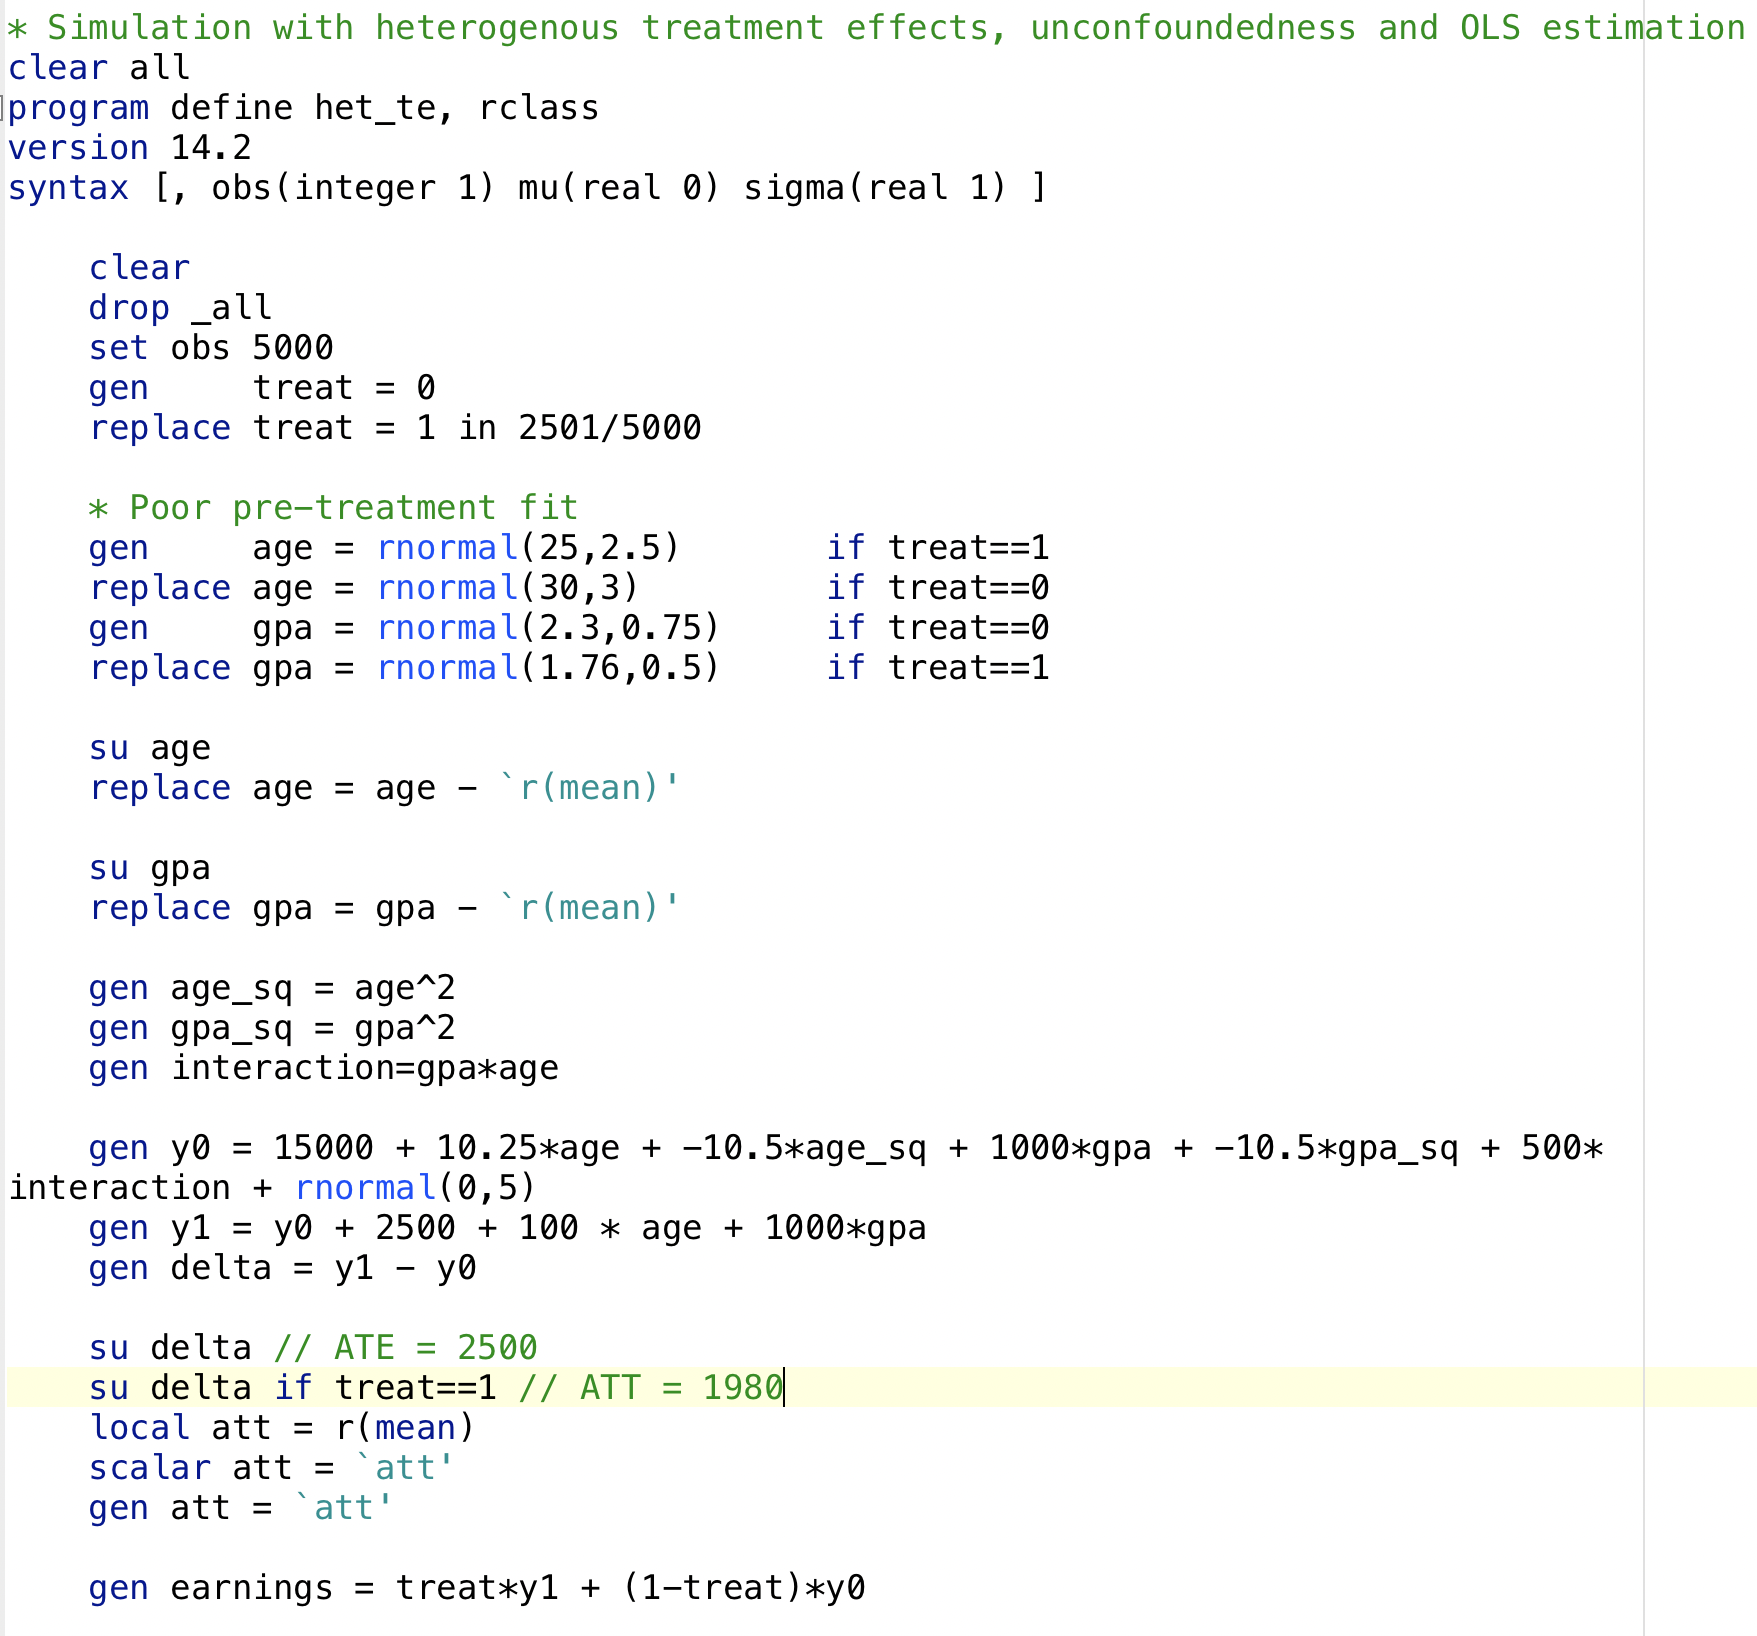
\includegraphics[scale=0.27]{./lecture_includes/stata_matching_code}
\end{figure}

\end{frame}

\begin{frame}{Parameters}

\begin{itemize}

\item Ordinarily we look at the coefficient on the treatment dummy to obtain an estimate
\item But we have two parameters: the ATE is \$2500 but the ATT is \$1980
\item How do we get both of them? Let's look at what people usually do
\item 1,000 simulations of DGP with regression estimates plotting coefficient on treatment dummy: first with just age and GPA, second with the precise model used for $Y^0$ (but not $Y^1$)

\end{itemize}

\end{frame}


\begin{frame}{Constant Treatment Effects and Linearity}

\begin{figure}[!t]\centering
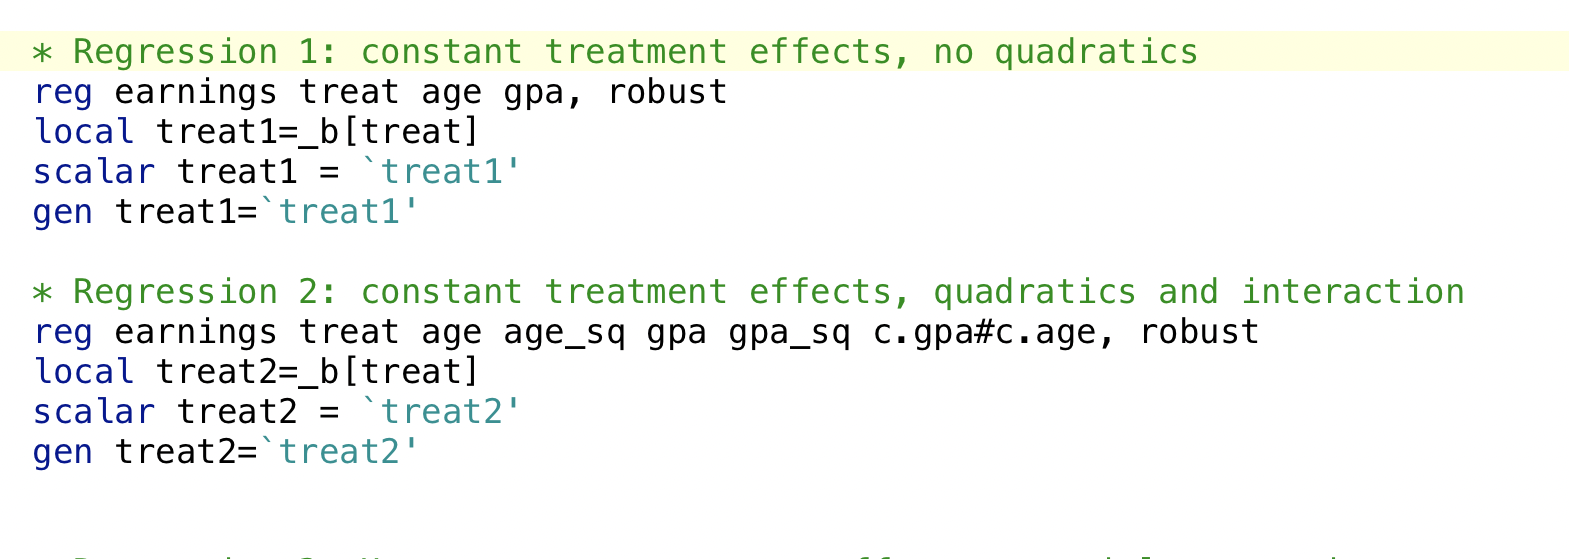
\includegraphics[scale=0.45]{./lecture_includes/stata_reg_constant}
\end{figure}

\end{frame}


\begin{frame}{Coefficient on Treatment Dummy is Wrong}

\begin{figure}[!t]\centering
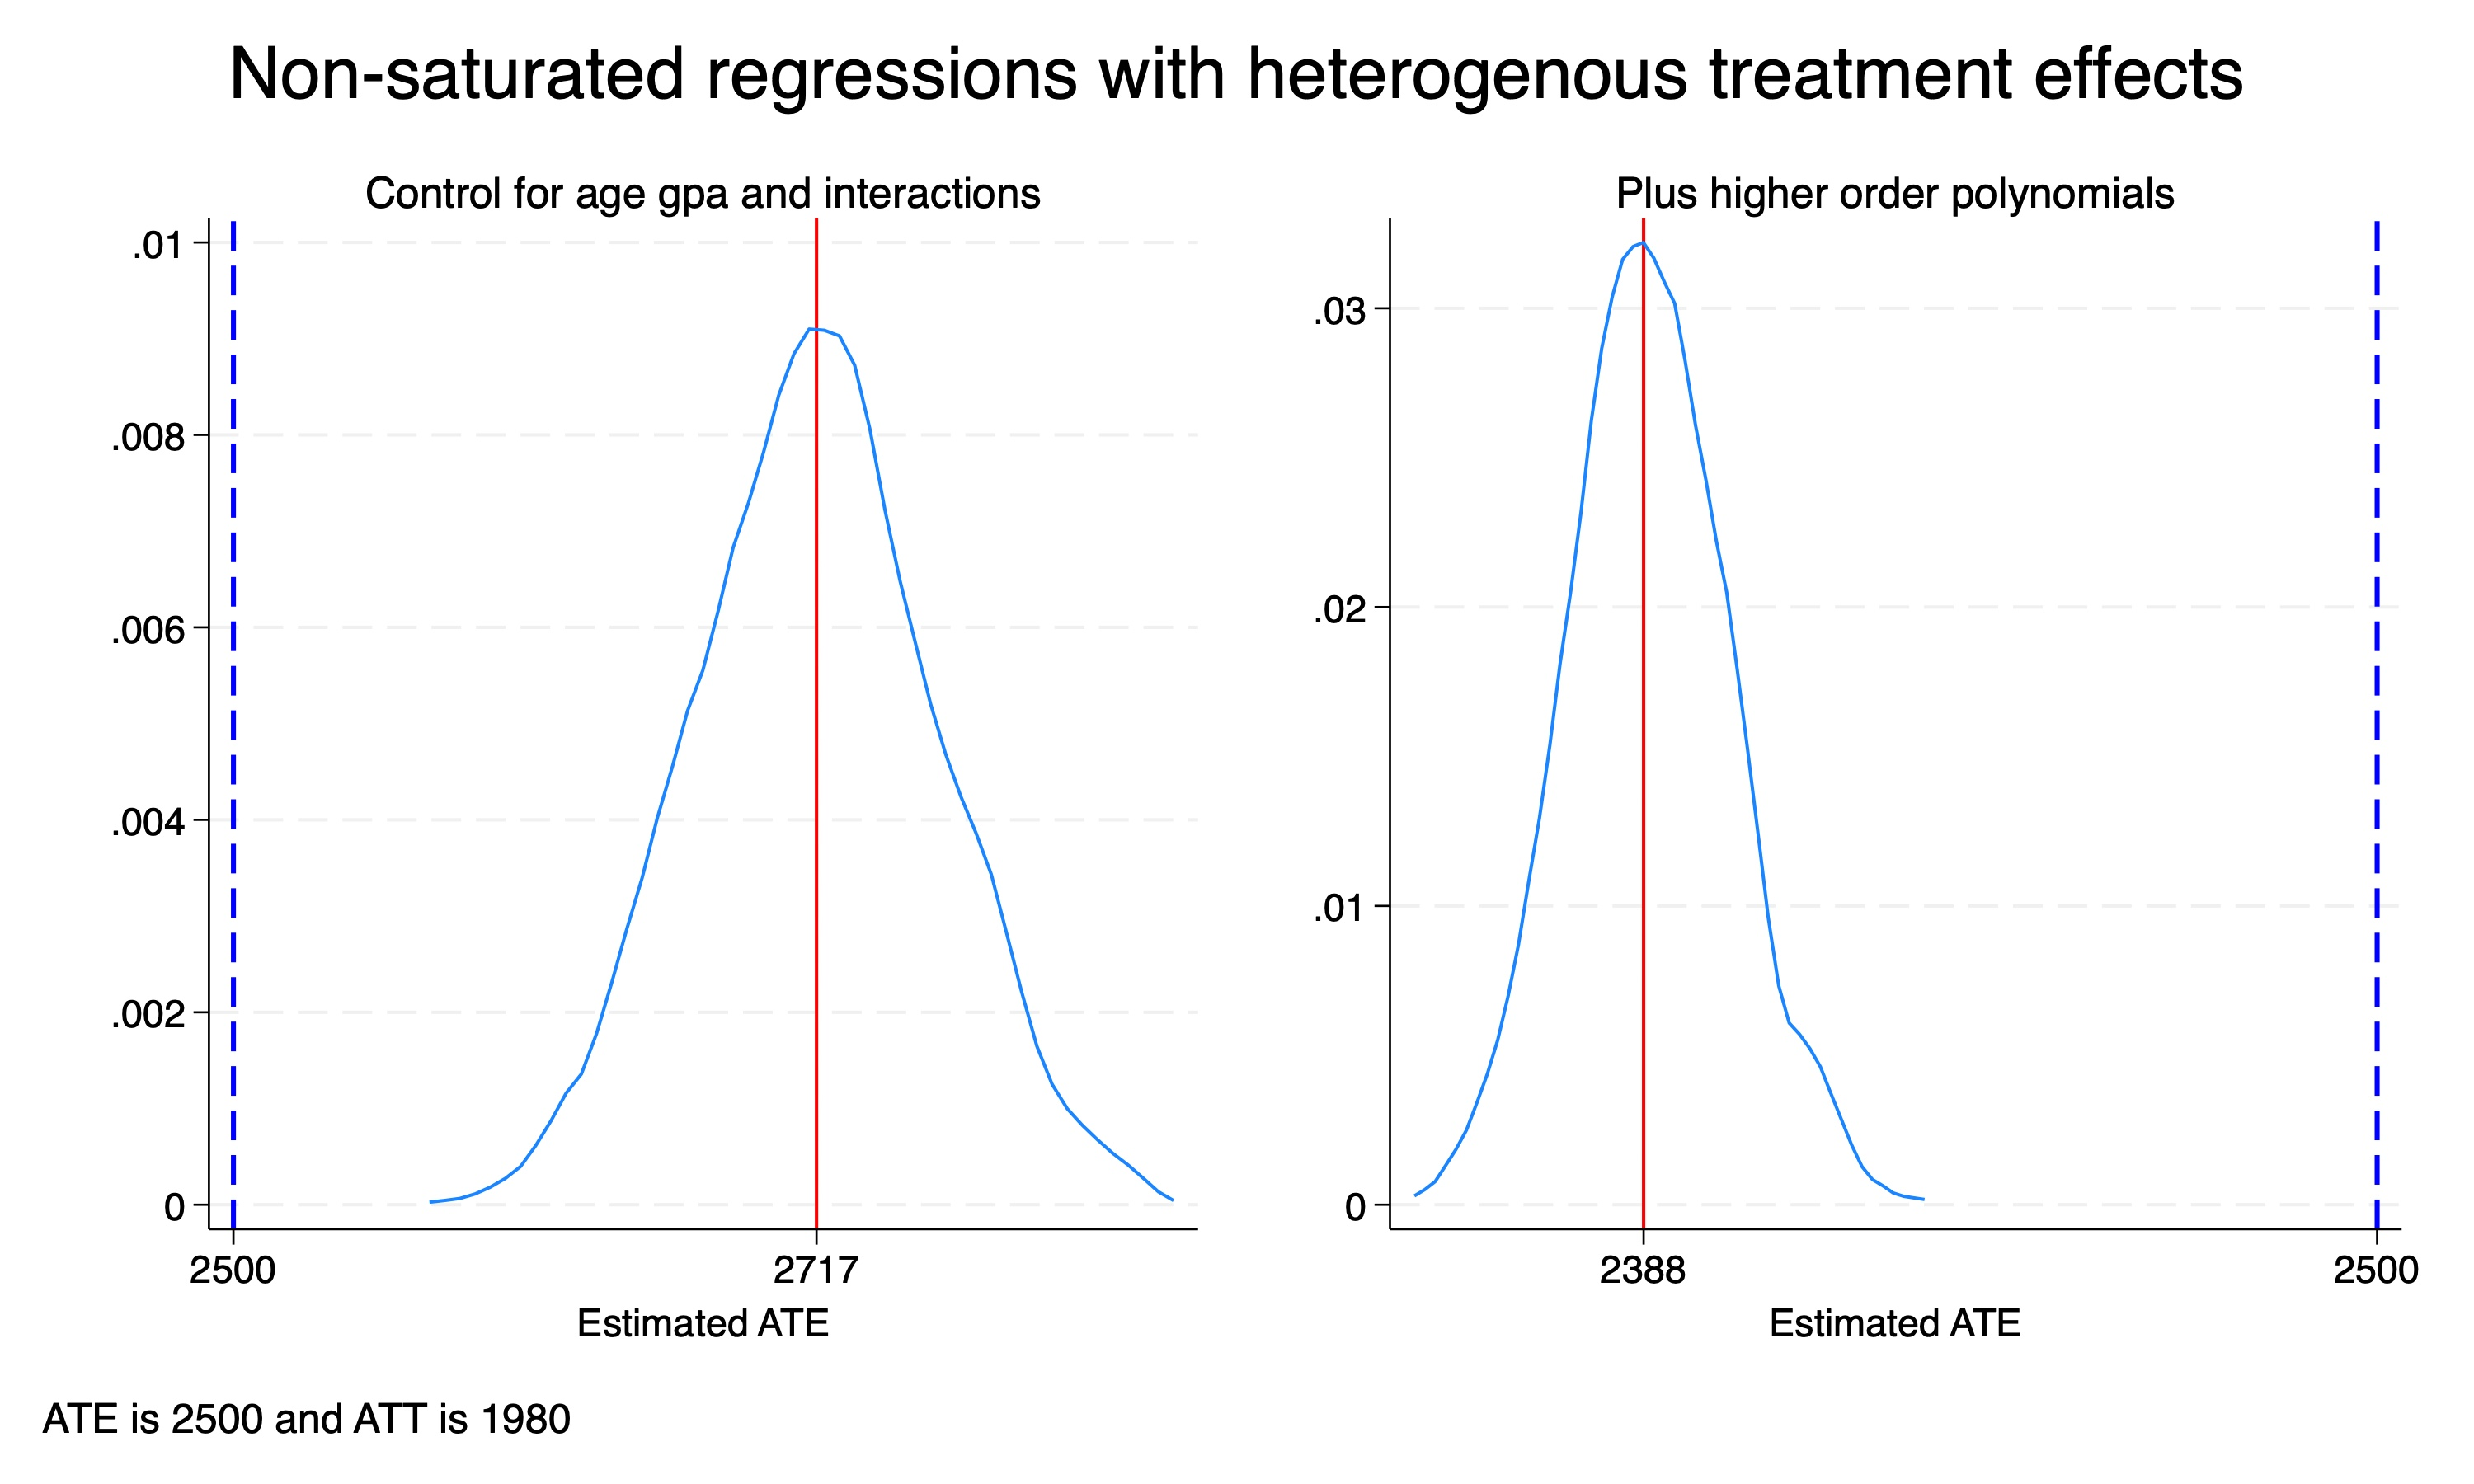
\includegraphics[scale=0.1]{./lecture_includes/combined_kernels.jpg}
\end{figure}

\end{frame}

\begin{frame}{Commentary}

\begin{itemize}

\item Three ifs and a then:

	\begin{itemize}
	\item \emph{If} unconfoundedness held, and 
	\item \emph{if} the potential outcome model was linear, and
	\item  \emph{if} the treatment effect had been homogenous with respect to age and GPA, 
	\item \emph{then} the coefficient on the treatment variable would have been the ATE 
	\end{itemize}
	
\item But it wasn't because homogeneity with respect to $X$ was not true (recall $Y(0)$ coefficients were not the same as $Y(1)$ coefficients)
\item So what had we done?  Bear with me but this will pay off
\end{itemize}

\end{frame}

\begin{frame}{Heterogenous treatment effects}

Write down a simplified version of the DGP from the code:

\begin{eqnarray*}
Y^0_i &=& \alpha + \beta_{01} X^0_i + \varepsilon_i \\
Y^1_i &=& \alpha + \beta_{01} X^0_i + \delta D_i + \beta_{11} X^1_i \times D_i + \varepsilon_i
\end{eqnarray*}

\bigskip

Notice that the setup before, $X_i$ had a different effect on $Y^0$ than it did on $Y_i^1$ -- that's because of heterogenous treatment effects with respect to conditioning set. 

\end{frame}

\begin{frame}{Heterogenous treatment x`effects}

Take conditional expectations of the \emph{potential} outcomes:

\begin{eqnarray*}
E[Y^0_i | D_i=1, X_i] &=& \alpha + \beta_{01} E[X^0_i] \\
E[Y^1_i | D_i=1, X_i] &=& \alpha + \beta_{01} E[X^0_i] + \delta + \beta_{11} E[X^1_i \times D_i | D_i=1,X_i^1]
\end{eqnarray*}

\bigskip

Average treatment effect is: 

\bigskip

\footnotesize

\begin{eqnarray*}
E[Y_i^1 | D_i, X^1_i] - E[Y^0_i | D_i, X^0_i] &=& \bigg (  \alpha + \beta_{01} E[X^0_i] + \delta + \beta_{11} E[X^1_i \times D_i | D_i=1,X_i^1] \bigg ) \\
&& -  \bigg (\alpha + \beta_{01} E[X^0_i] \bigg ) \\
&=& \delta + \beta_{11}  E[X^1_i | D_i=1] 
\end{eqnarray*}assuming $X^1_i=X^0_i$. OLS model accounting for heterogeneity must be ``fully saturated''.


\end{frame}




\begin{frame}{Estimation}

Our saturated OLS model is:

\bigskip

\begin{eqnarray*}
Y_i = \alpha + \delta D_i + \beta_{01} X_i + \beta_{11} D_i \times X_i + \varepsilon_i
\end{eqnarray*}

$\widehat{\delta}$ is the ATE but the ATT is equal to $\widehat{\delta} + \beta_{11} E[X_i | D_i = 1]$ where $E[X_i | D_i=1]$ is the sample average of $X_i$ for the treatment group

\bigskip

We will estimate two models: (1) once with simplified but incorrectly specified saturated and (2) another with the correctly specified saturated model -- warning, it's a huge pain and you can easily mess it up even with just a few variables

\end{frame}



\begin{frame}{Misspecified Saturated OLS Regression}

\begin{figure}[!t]\centering
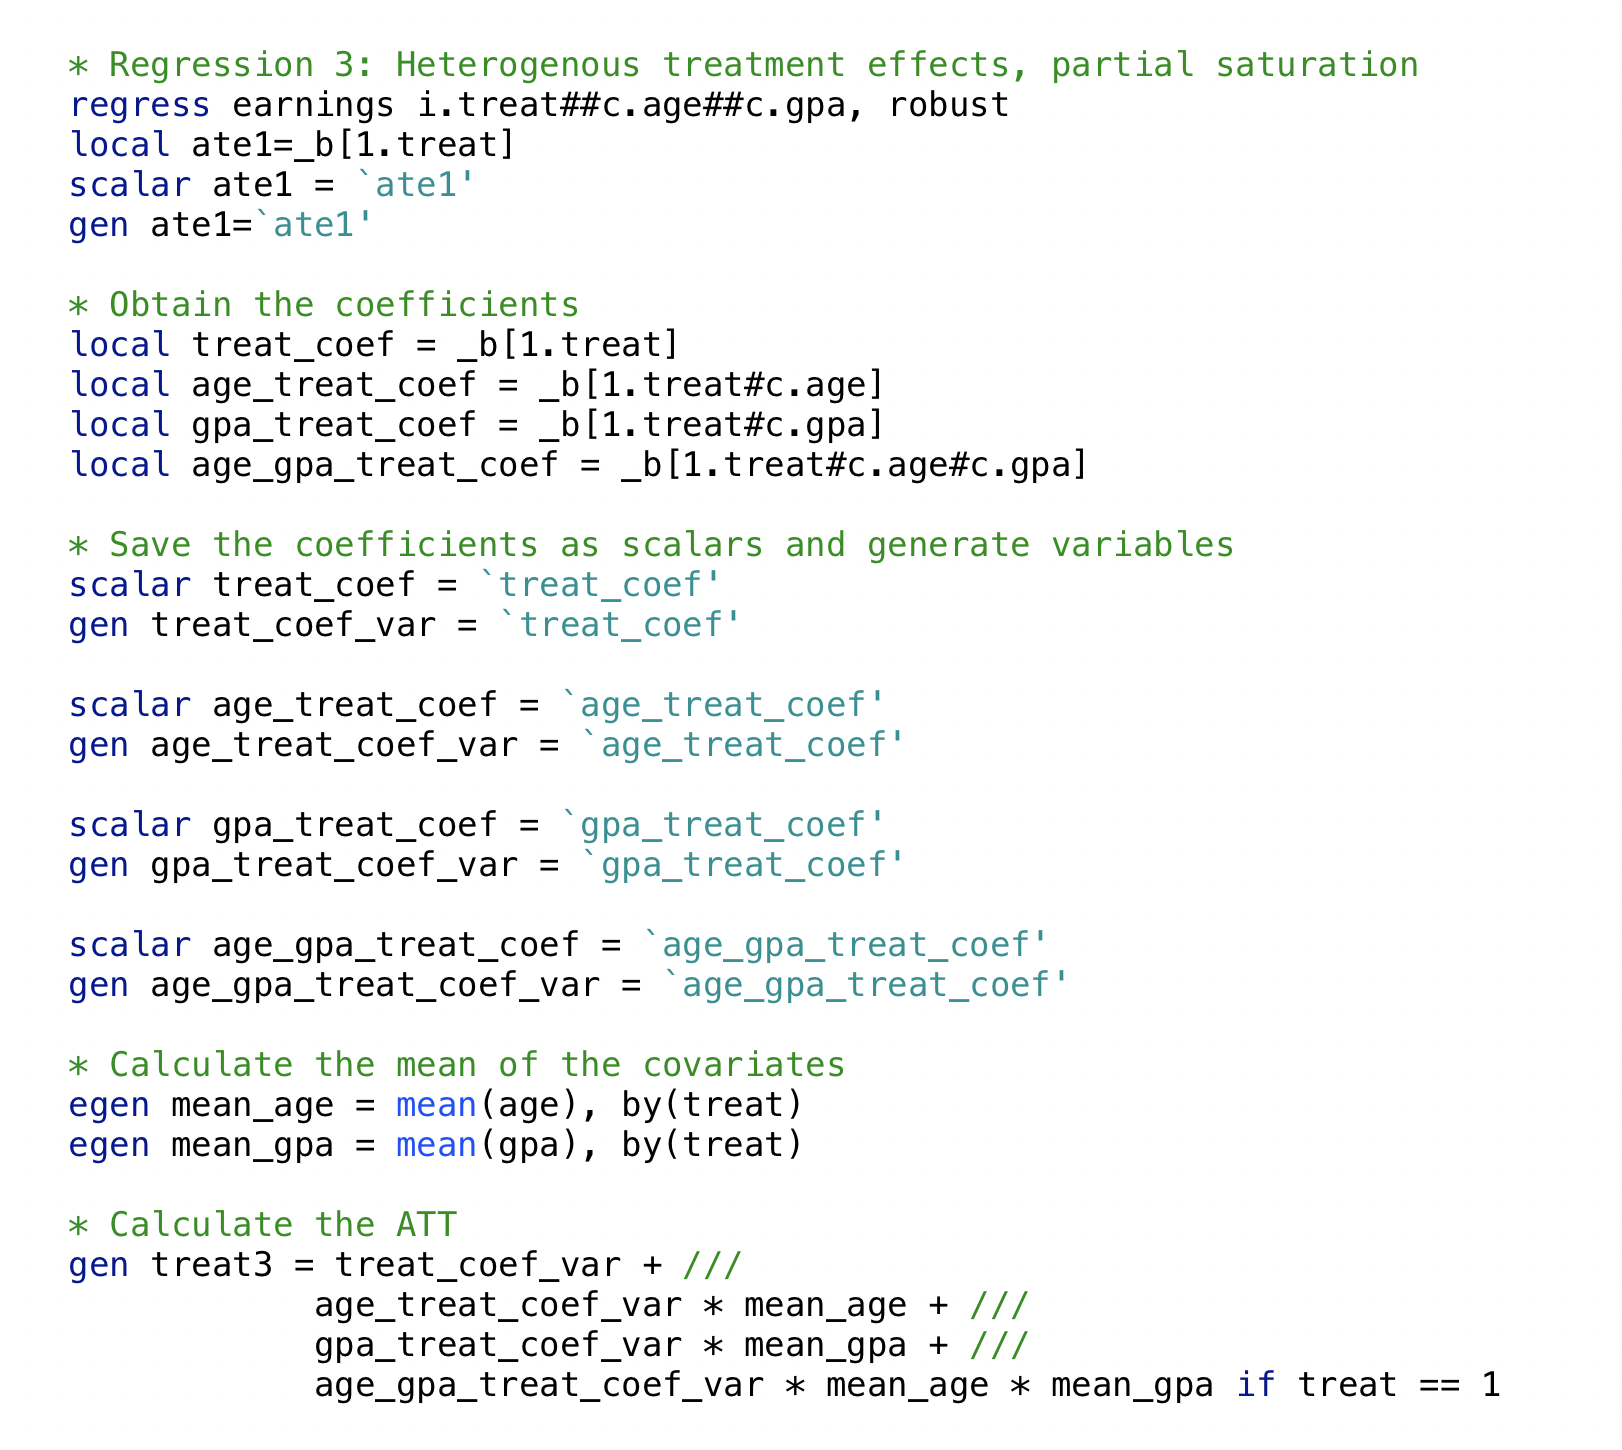
\includegraphics[scale=0.3]{./lecture_includes/saturated_reg3}
\end{figure}

\end{frame}


\begin{frame}{Misspecified Saturated OLS Regression}

\begin{figure}[!t]\centering
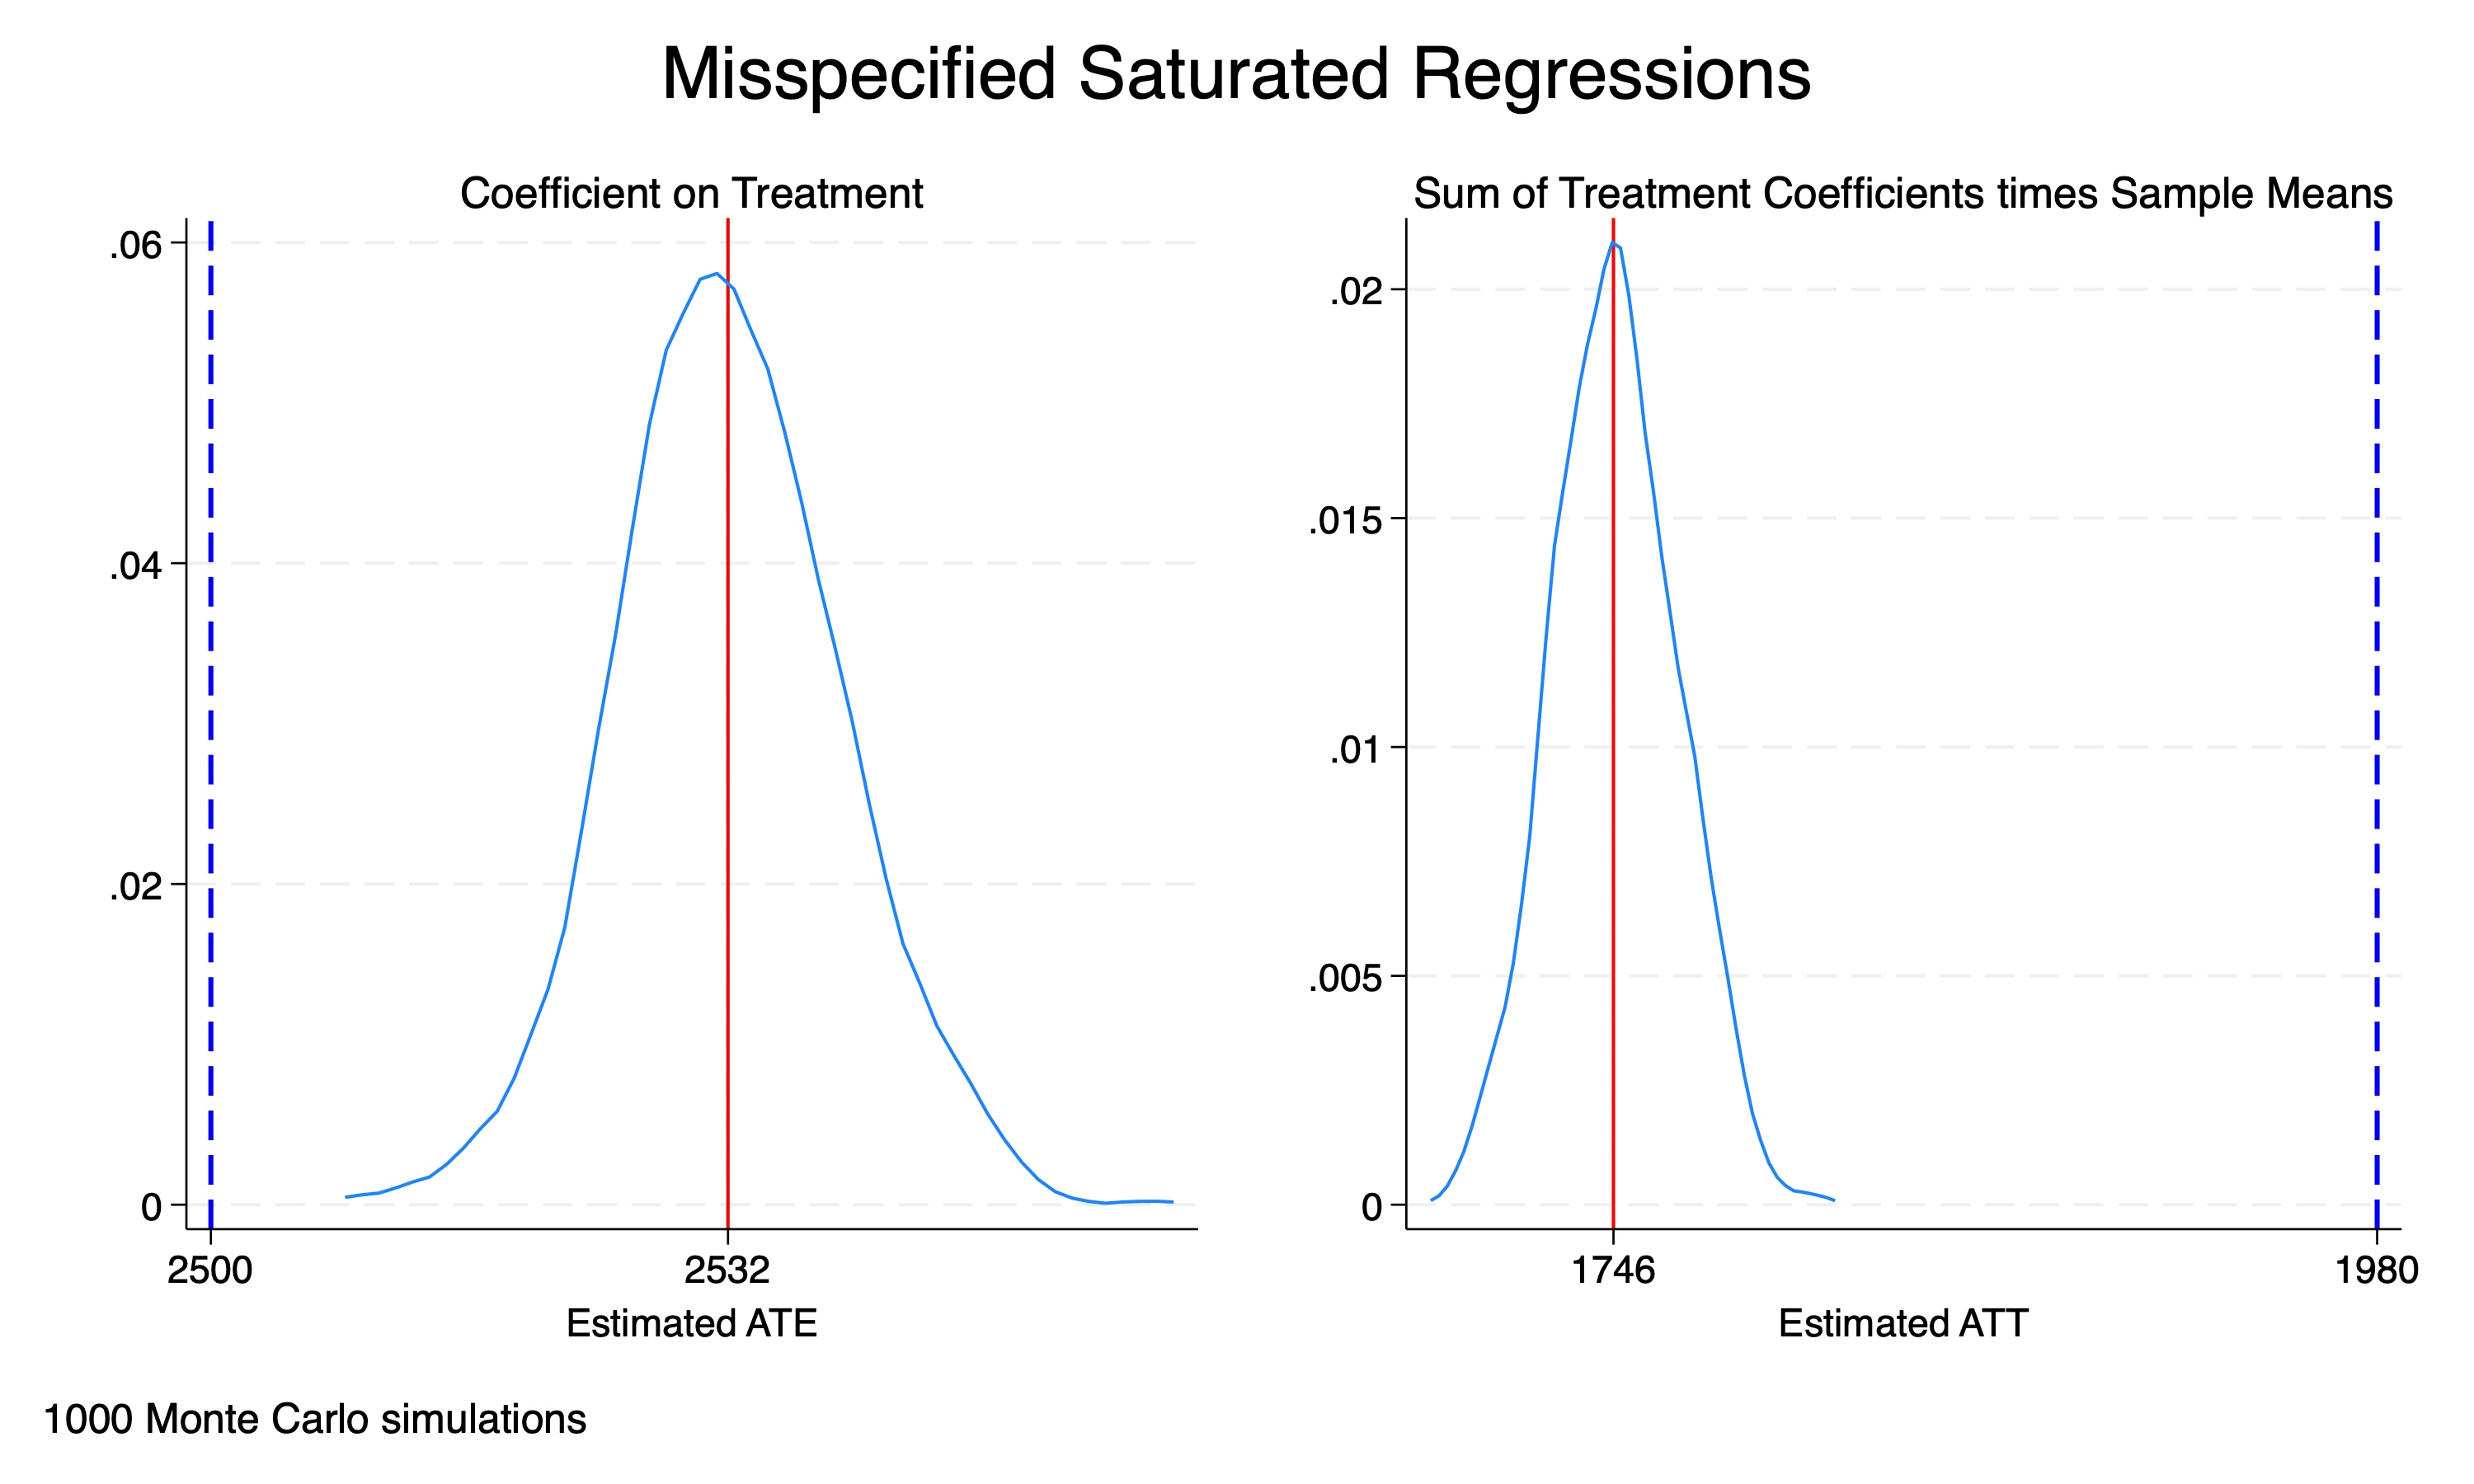
\includegraphics[scale=0.1]{./lecture_includes/combined_saturated1.jpg}
\end{figure}

\end{frame}

\begin{frame}{Comically Long Saturated OLS Regression}

\begin{figure}[!t]\centering
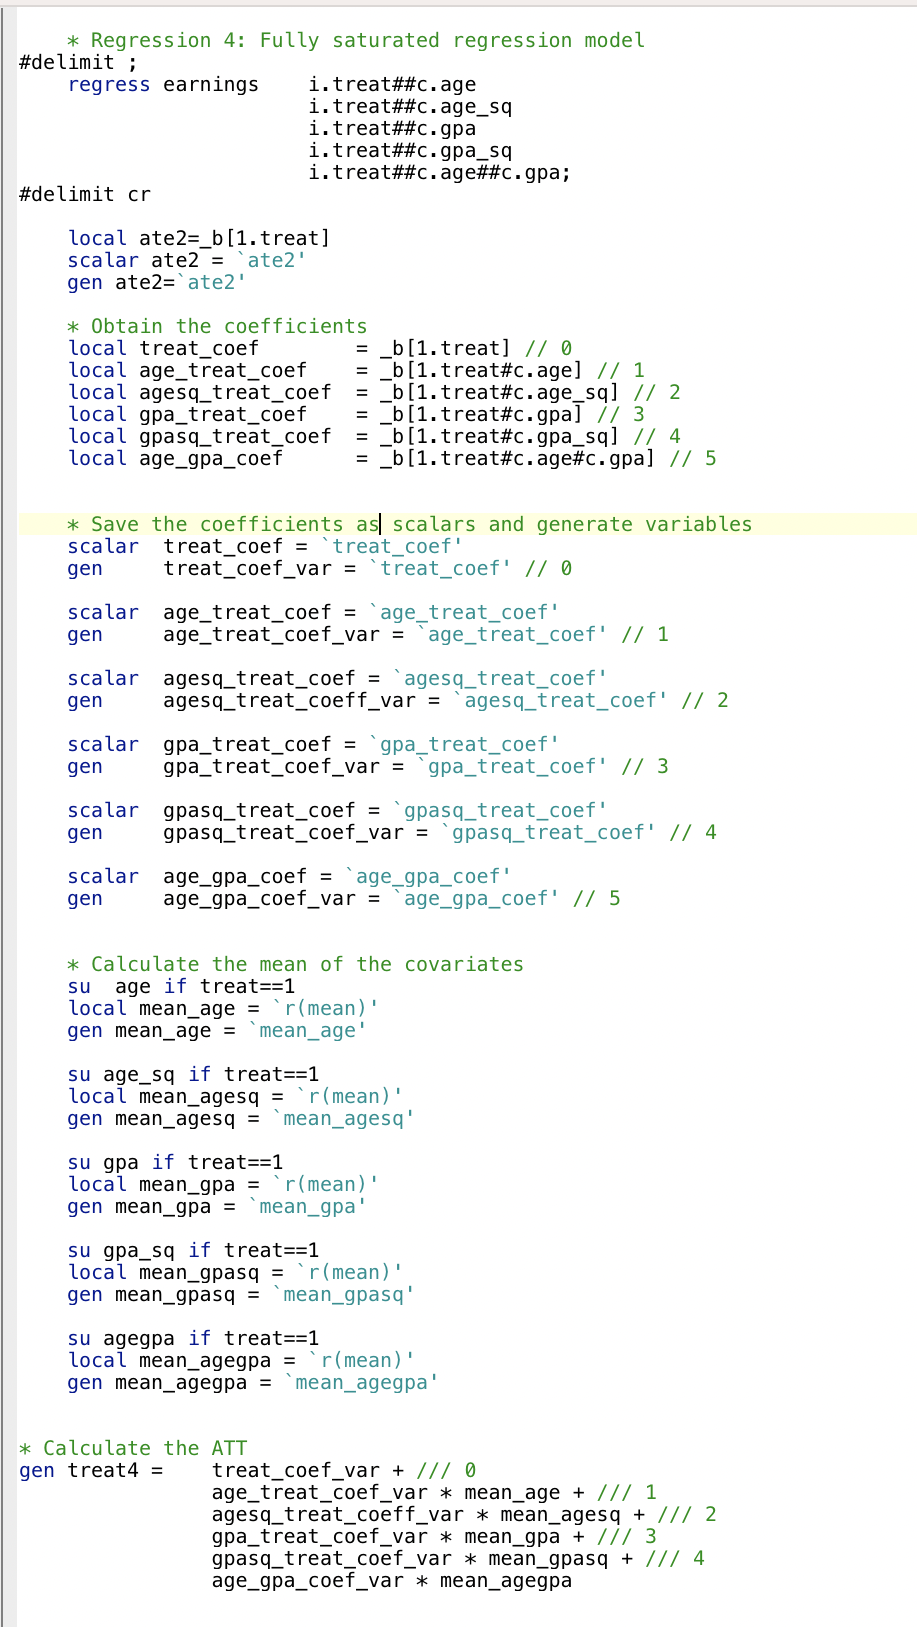
\includegraphics[scale=0.26]{./lecture_includes/stata_full_code}
\end{figure}

\end{frame}

\begin{frame}{Correctly Saturated OLS Regression}

\begin{figure}[!t]\centering
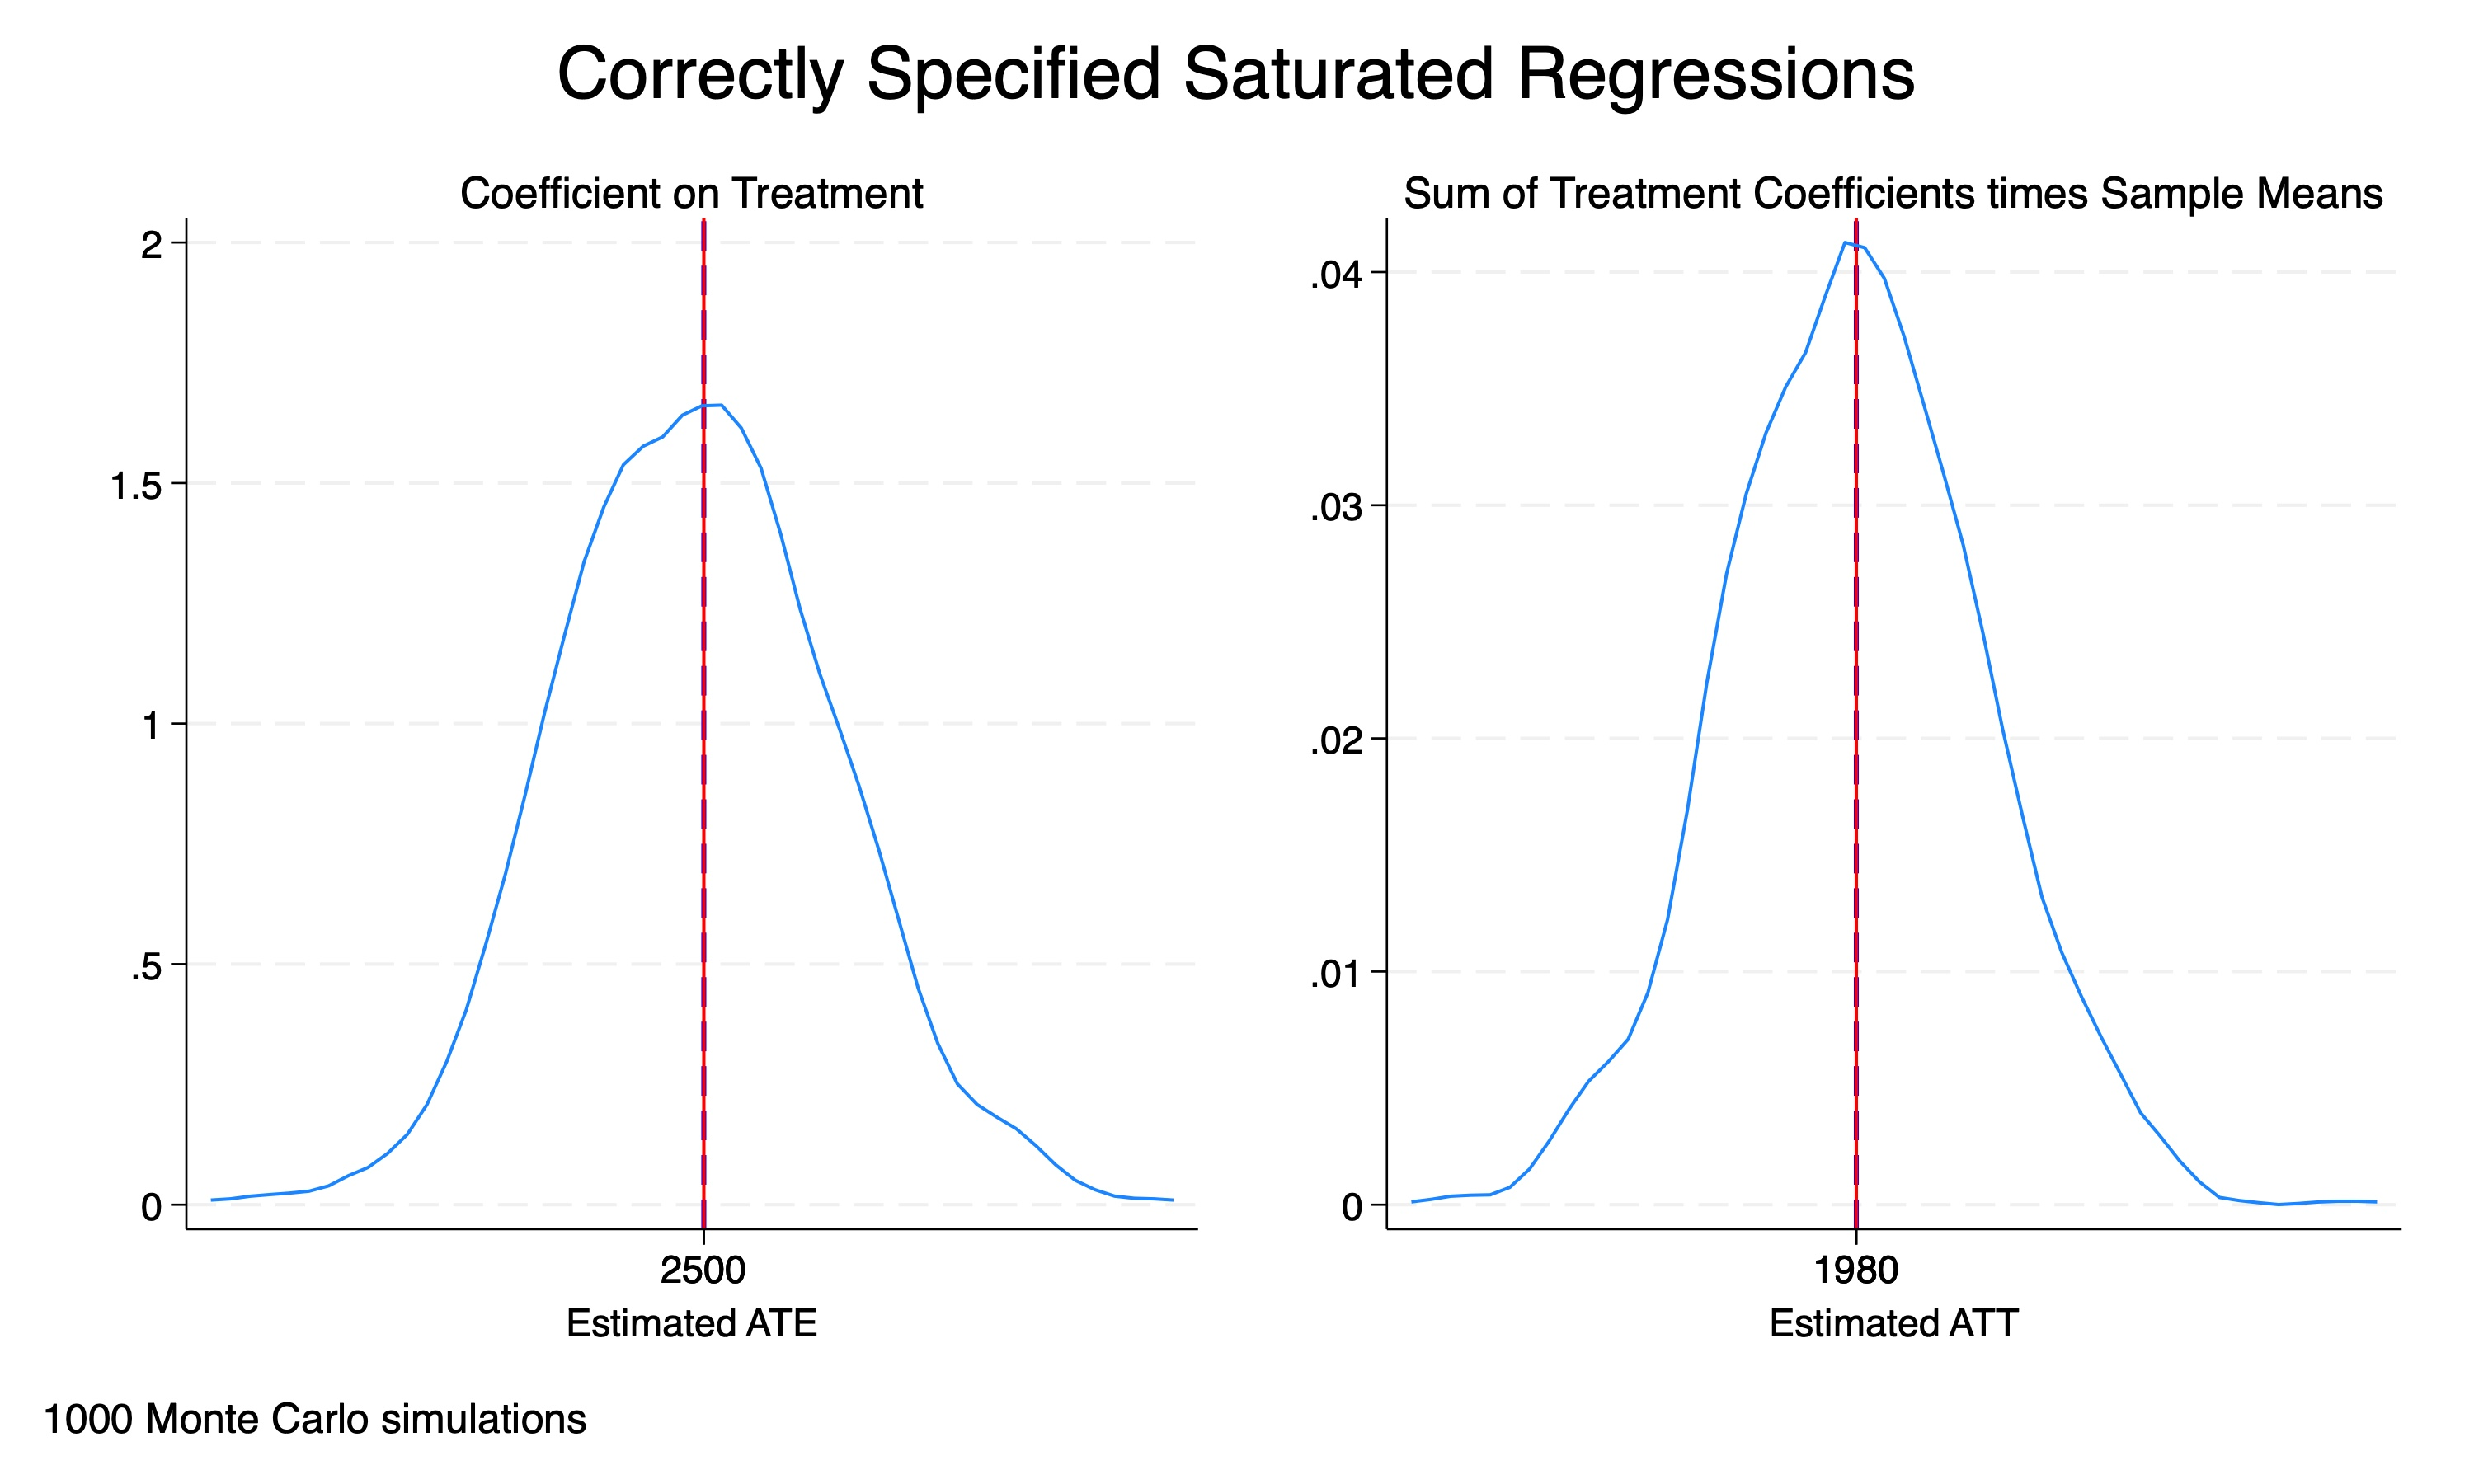
\includegraphics[scale=0.1]{./lecture_includes/combined_saturated2.jpg}
\end{figure}

\end{frame}


\begin{frame}{Matching}

\begin{itemize}

\item Now let's estimate the ATT (\$1980) using nearest neighbor matching by minimizing Mahalanobis distance on age, GPA, polynomials and interaction
\item One line in Stata using \texttt{teffects} and only 1 match (variance is simple to estimate until we use matches multiple times, then the variance grows)
\item In R, the package is \texttt{Matching}, not sure in python
\end{itemize}

\end{frame}


\begin{frame}{Matching Estimation}

\begin{figure}[!t]\centering
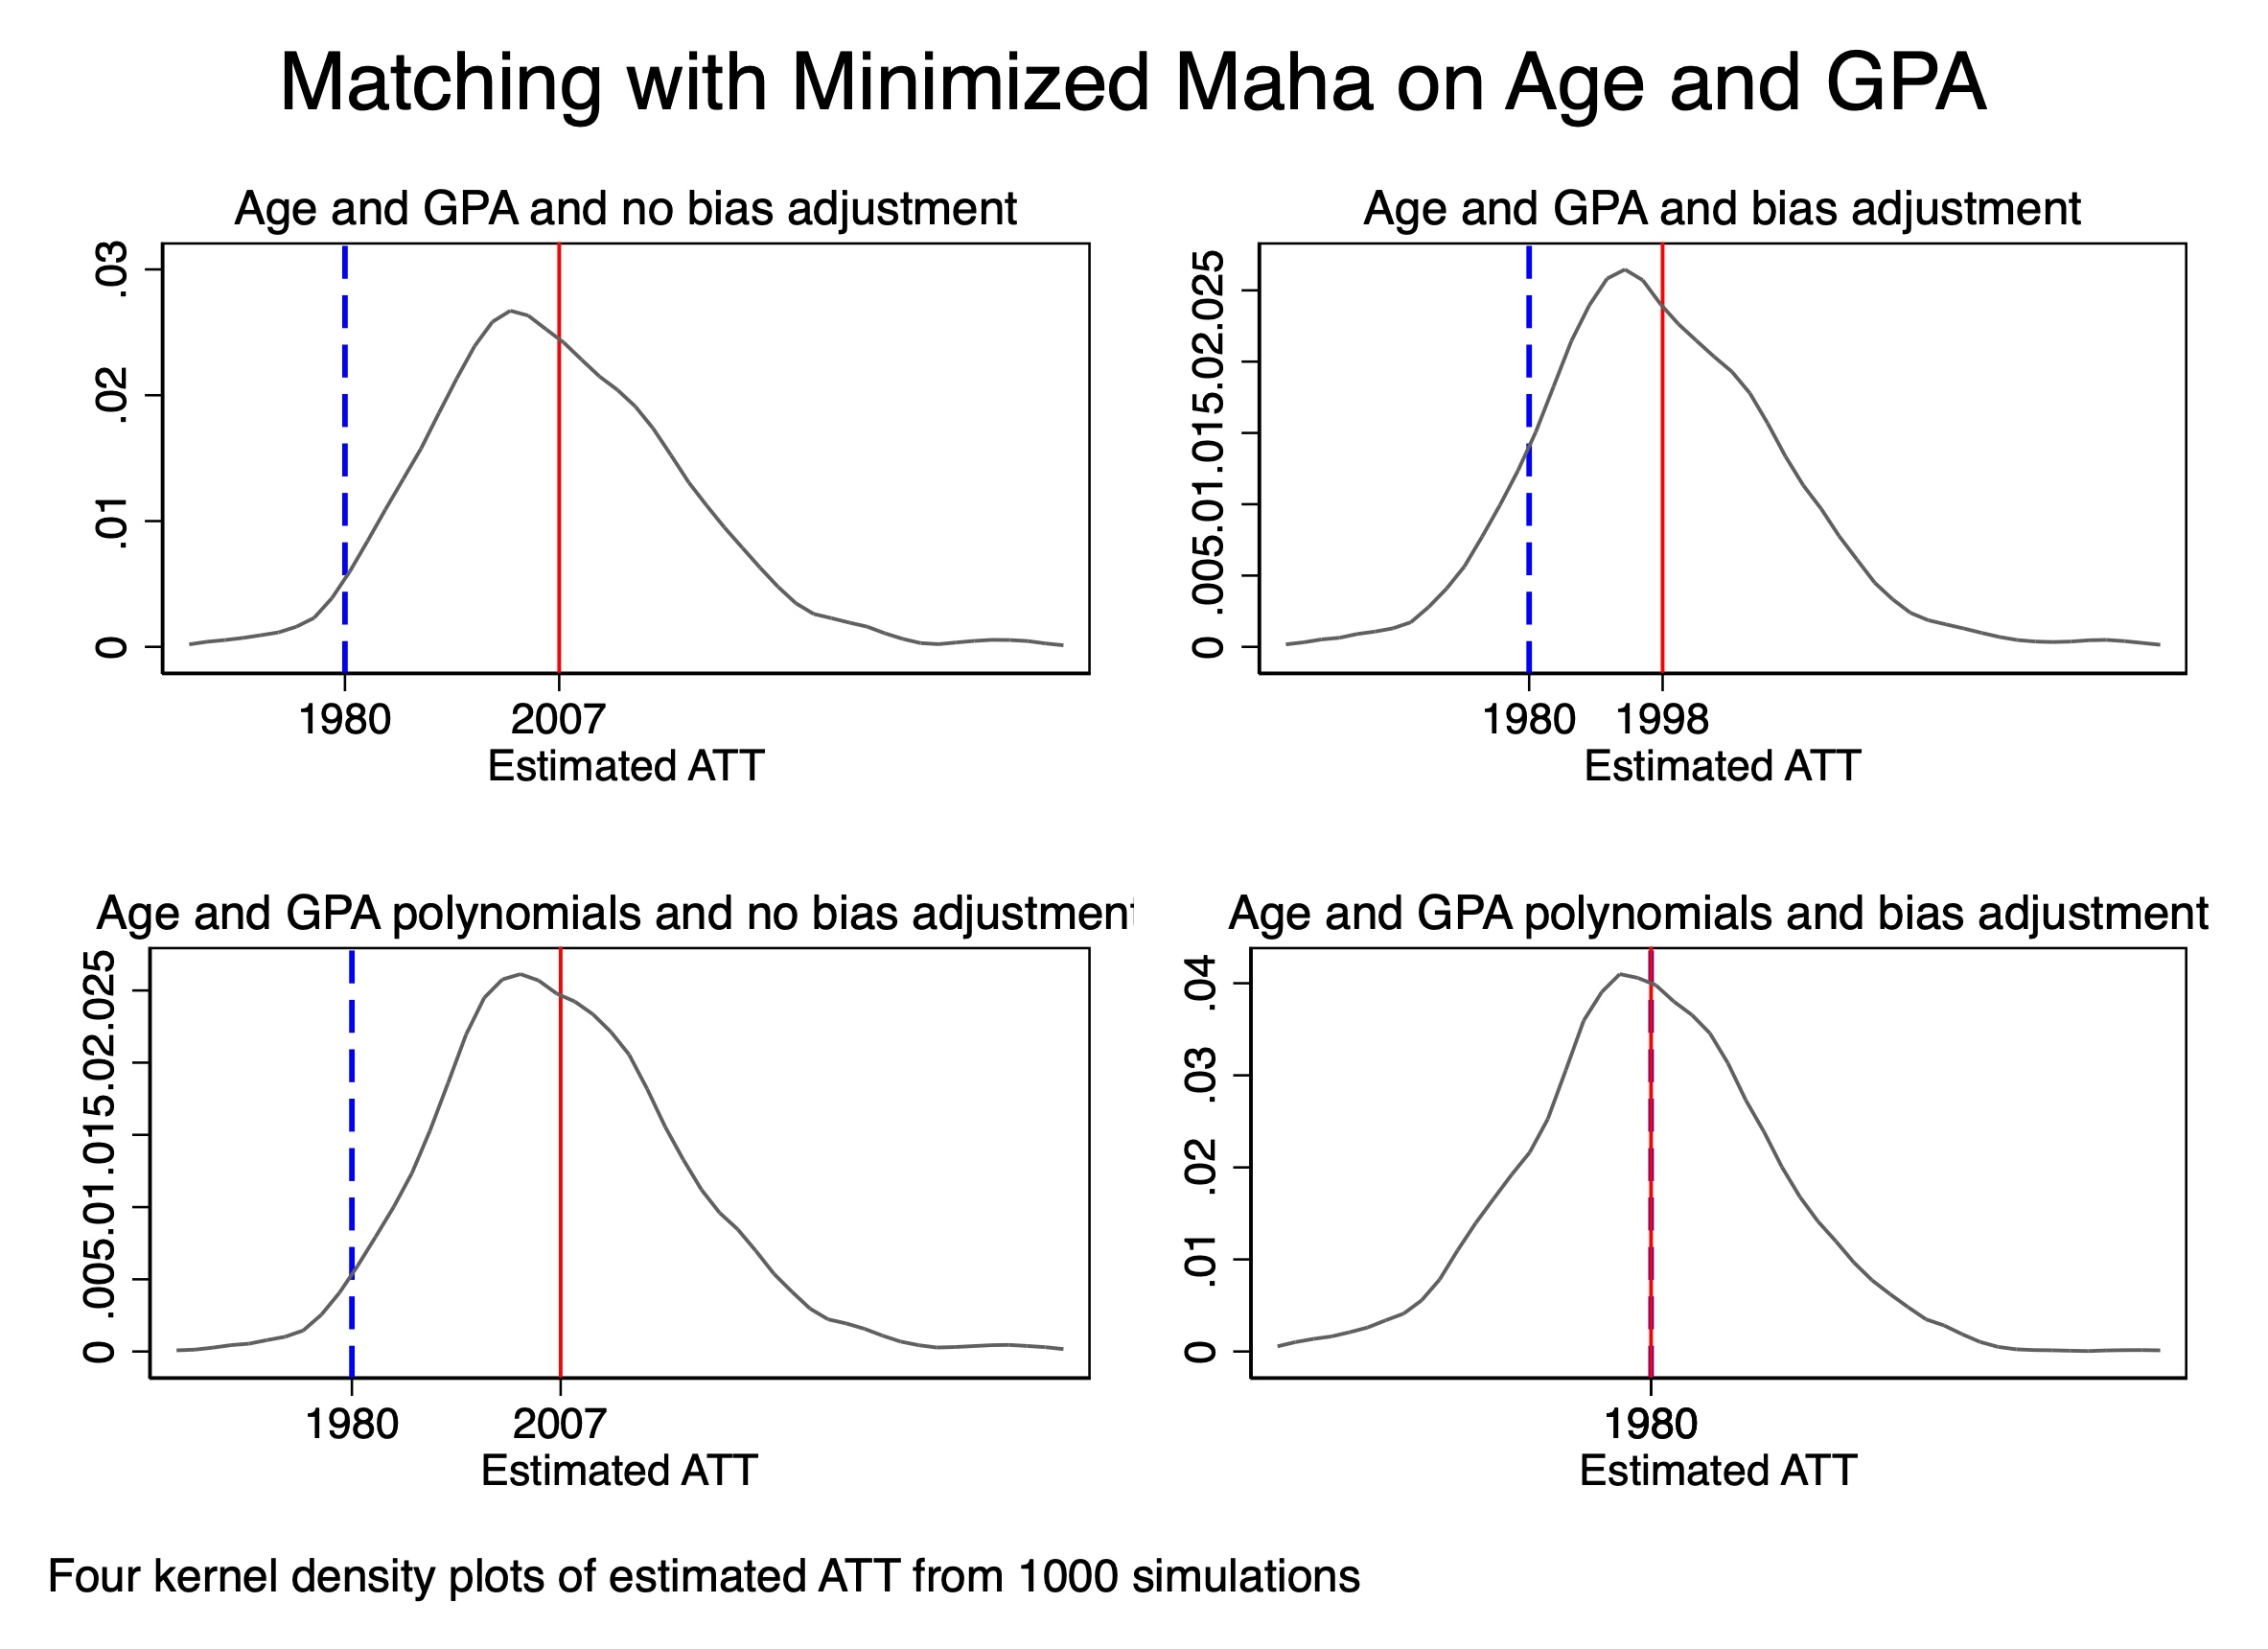
\includegraphics[scale=0.1]{./lecture_includes/combined_kernels_maha.jpg}
\end{figure}

\end{frame}

\begin{frame}{Commentary}

\begin{itemize}
\item Full saturation tips -- remember to center the covariates at the start, be sure to specify ahead of time which parameter (ATT or ATE) and note that the covariates must not be based on the treatment (``exogenous'' and confounders only)
\item Other methods, more sophisticated, have emerged such as outcome regressions where you impute missing counterfactuals, $\widehat{E[Y^0|D=1,X]}$ using the comparison group only and $Y^0$ as a function of $X$ 
\item But note the saturation is not merely so you can examine heterogeneity at the margin -- you need it even to get the correct ATE as we saw which is distinct from the ATT
\end{itemize}

\end{frame}




\begin{frame}{Commentary}

\begin{itemize}

\item Unconfoundedness requires that you \emph{know} and \emph{include} all confounders to adjust comparisons when estimating treatment effects
\item Without a prior behavioral model guiding you, it's very hard to defend conditional independence (borderline disingenuous) 
\item If you are unwilling to use DAGs, you may want to ask yourself why you are comfortable running regressions with covariates?

\end{itemize}

\end{frame}

\begin{frame}{Avoiding dimensionality problems}
	
	\begin{itemize}
	\item Rubin (1977) and Rosenbaum and Rubin (1983) developed the propensity score method which is a dimension reduction method of reducing $K$ covariates used for adjusting into a single scalar called the propensity score
	\item Propensity score is simply the frequentist share of units in the treatment group with values of $X$ compared to all units with values of $X$
	\item Can be then used to weight conditional mean outcomes of the comparison group to get the ATT as well as match, but I'm going to focus on weighting
	\end{itemize}
	
\end{frame}






\begin{frame}{Basic idea behind propensity scores}
	
	\begin{itemize}
	\item Earlier we matched on $X$'s to compare units ``near'' one another based on some distance but matching discrepancies and sparseness created problems
	\item Propensity scores summarize covariate information about treatment selection into a single number bounded between 0 and 1 (i.e., a probability)
	\item Rather than compare units with similar values of $X$, we compare units with similar \textbf{estimated conditional probabilities of treatment}
	\item Important theorem shows that once we adjust comparisons using the propensity score, we do not need to adjust for $X$
	\end{itemize}
\end{frame}



\begin{frame}{Formal Definition}
	
	\begin{block}{Definition of Propensity score}
	A propensity score is a number bounded between 0 and 1 measuring the probability of treatment assignment conditional on a vector of confounding variables: $p(X)=Pr(D=1 | X)$
	\end{block}
	
	\bigskip
	
	For the ATT, we need weak unconfoundedness and weak overlap (i.e., only need overlap for the treatment group)

\end{frame}

\begin{frame}{Propensity score theorem}
	
	\begin{block}{Propensity score theorem}
	If $(Y^1,Y^0)\independent{D}|X$ (unconfoundedness), then $(Y^1,Y^0)\independent{D} | \rho(X)$ where $\rho(X)=Pr(D=1|X)$, the propensity score
	\end{block}
	
	\begin{itemize}
	\item Conditioning on the propensity score is enough to have independence between $D$ and $(Y^1,Y^0)$ (Rosenbaum and Rubin 1983)
	 \item Valuable theorem because of dimension reduction and convergence rate issues which can introduce biases
	\end{itemize}
\end{frame}



\begin{frame}{Step 1: Estimate the propensity score}

		\begin{itemize}
		\item Estimate the conditional probability of treatment using probit or logit model (or more sophisticated) $$Pr(D_i=1|X_i) = F(\beta X_i)$$
		\item Use the estimated coefficients to calculate the propensity score for each unit $i$$$\widehat{\rho}_i(X_i) = \widehat{\beta} X_i$$
		\item Note that each unit $i$ now has a predicted probability of treatment given the values of their covariates relative to everyone else's 
		\item Frequentist probability -- you've basically just obtained the likelihood someone who ``looks like you'' would be treated (regardless of whether you were in fact treated)
		\end{itemize}
\end{frame}




\begin{frame}{Step 2: Estimation of ATT with IPW}

\begin{itemize}
	\item IPW uses the estimated propensity score to reweight the outcomes (e.g., Robins and Rotnitzky 1995, Imbens 2000, Hirano and Imbens 2001)
	\item IPW is non-parametric -- you are just taking averages and multiplying by weights
	\item There are also fewer implementation choices -- you aren't choosing how many neighbors to include, how far away a neighbor can be -- but you still have to closely examine common support
	\item There are bias adjustment methods called double robust where you combine imputing counterfactuals with weighting by the propensity score
\end{itemize}

\end{frame}
	
	

\begin{frame}{Step 2: Estimation of ATT with IPW}
	
		\begin{block}{Estimating ATT with IPW}
	Given $Y^0 \independent{D}|X$ and common support, then
		\begin{eqnarray*}
		\delta_{ATT}&=&E[Y^1-Y^0|D=1] \\
		&=& \frac{1}{Pr(D=1)} \cdot  E \left[ Y \cdot \frac{D-\rho(X)}{1-\rho(X)} \right]
		\end{eqnarray*}
	\end{block}Notice that when $D=1$, the outcome is not weighted, but when $D=0$ it is. You're missing the $Y^0$ for the treatment, not $Y^1$ so you the treatment group $Y$ values alone and weight ``up'' or ``down'' the comparison groups by their propensity scores

\end{frame}


\begin{frame}{Step 3: Standard Errors}
	
		
Standard errors can be constructed a few different ways:
	\begin{itemize}
	\item We need to adjust the standard errors for first-step estimation of $\rho(X)$
		\begin{itemize}
		\item Parameteric first step: Newey and McFadden (1994)
		\item Non-parametric first step: Newey (1994)
		\end{itemize}
	\item IPW is a smooth estimator which means the bootstrap is valid for inference  (Adudumilli 2018 and Bodory et al. 2020) 
	\end{itemize}
\end{frame}


\begin{frame}{Practical uses}

\begin{itemize}

\item One of the things I find immensely valuable is that when you can collapse the conditioning set into a single scalar, then assessing overlap is simple
\item Just create histograms of the propensity score distribution for treatment and control
\item Crump, et al. (2009) suggest keeping propensity scores within the interval [0.1,0.9] (``trimming'') but note any time you drop a unit, you are moving away from the ATT

\end{itemize}

\end{frame}

\begin{frame}{Assessing overlap}

\begin{figure}[!t]\centering
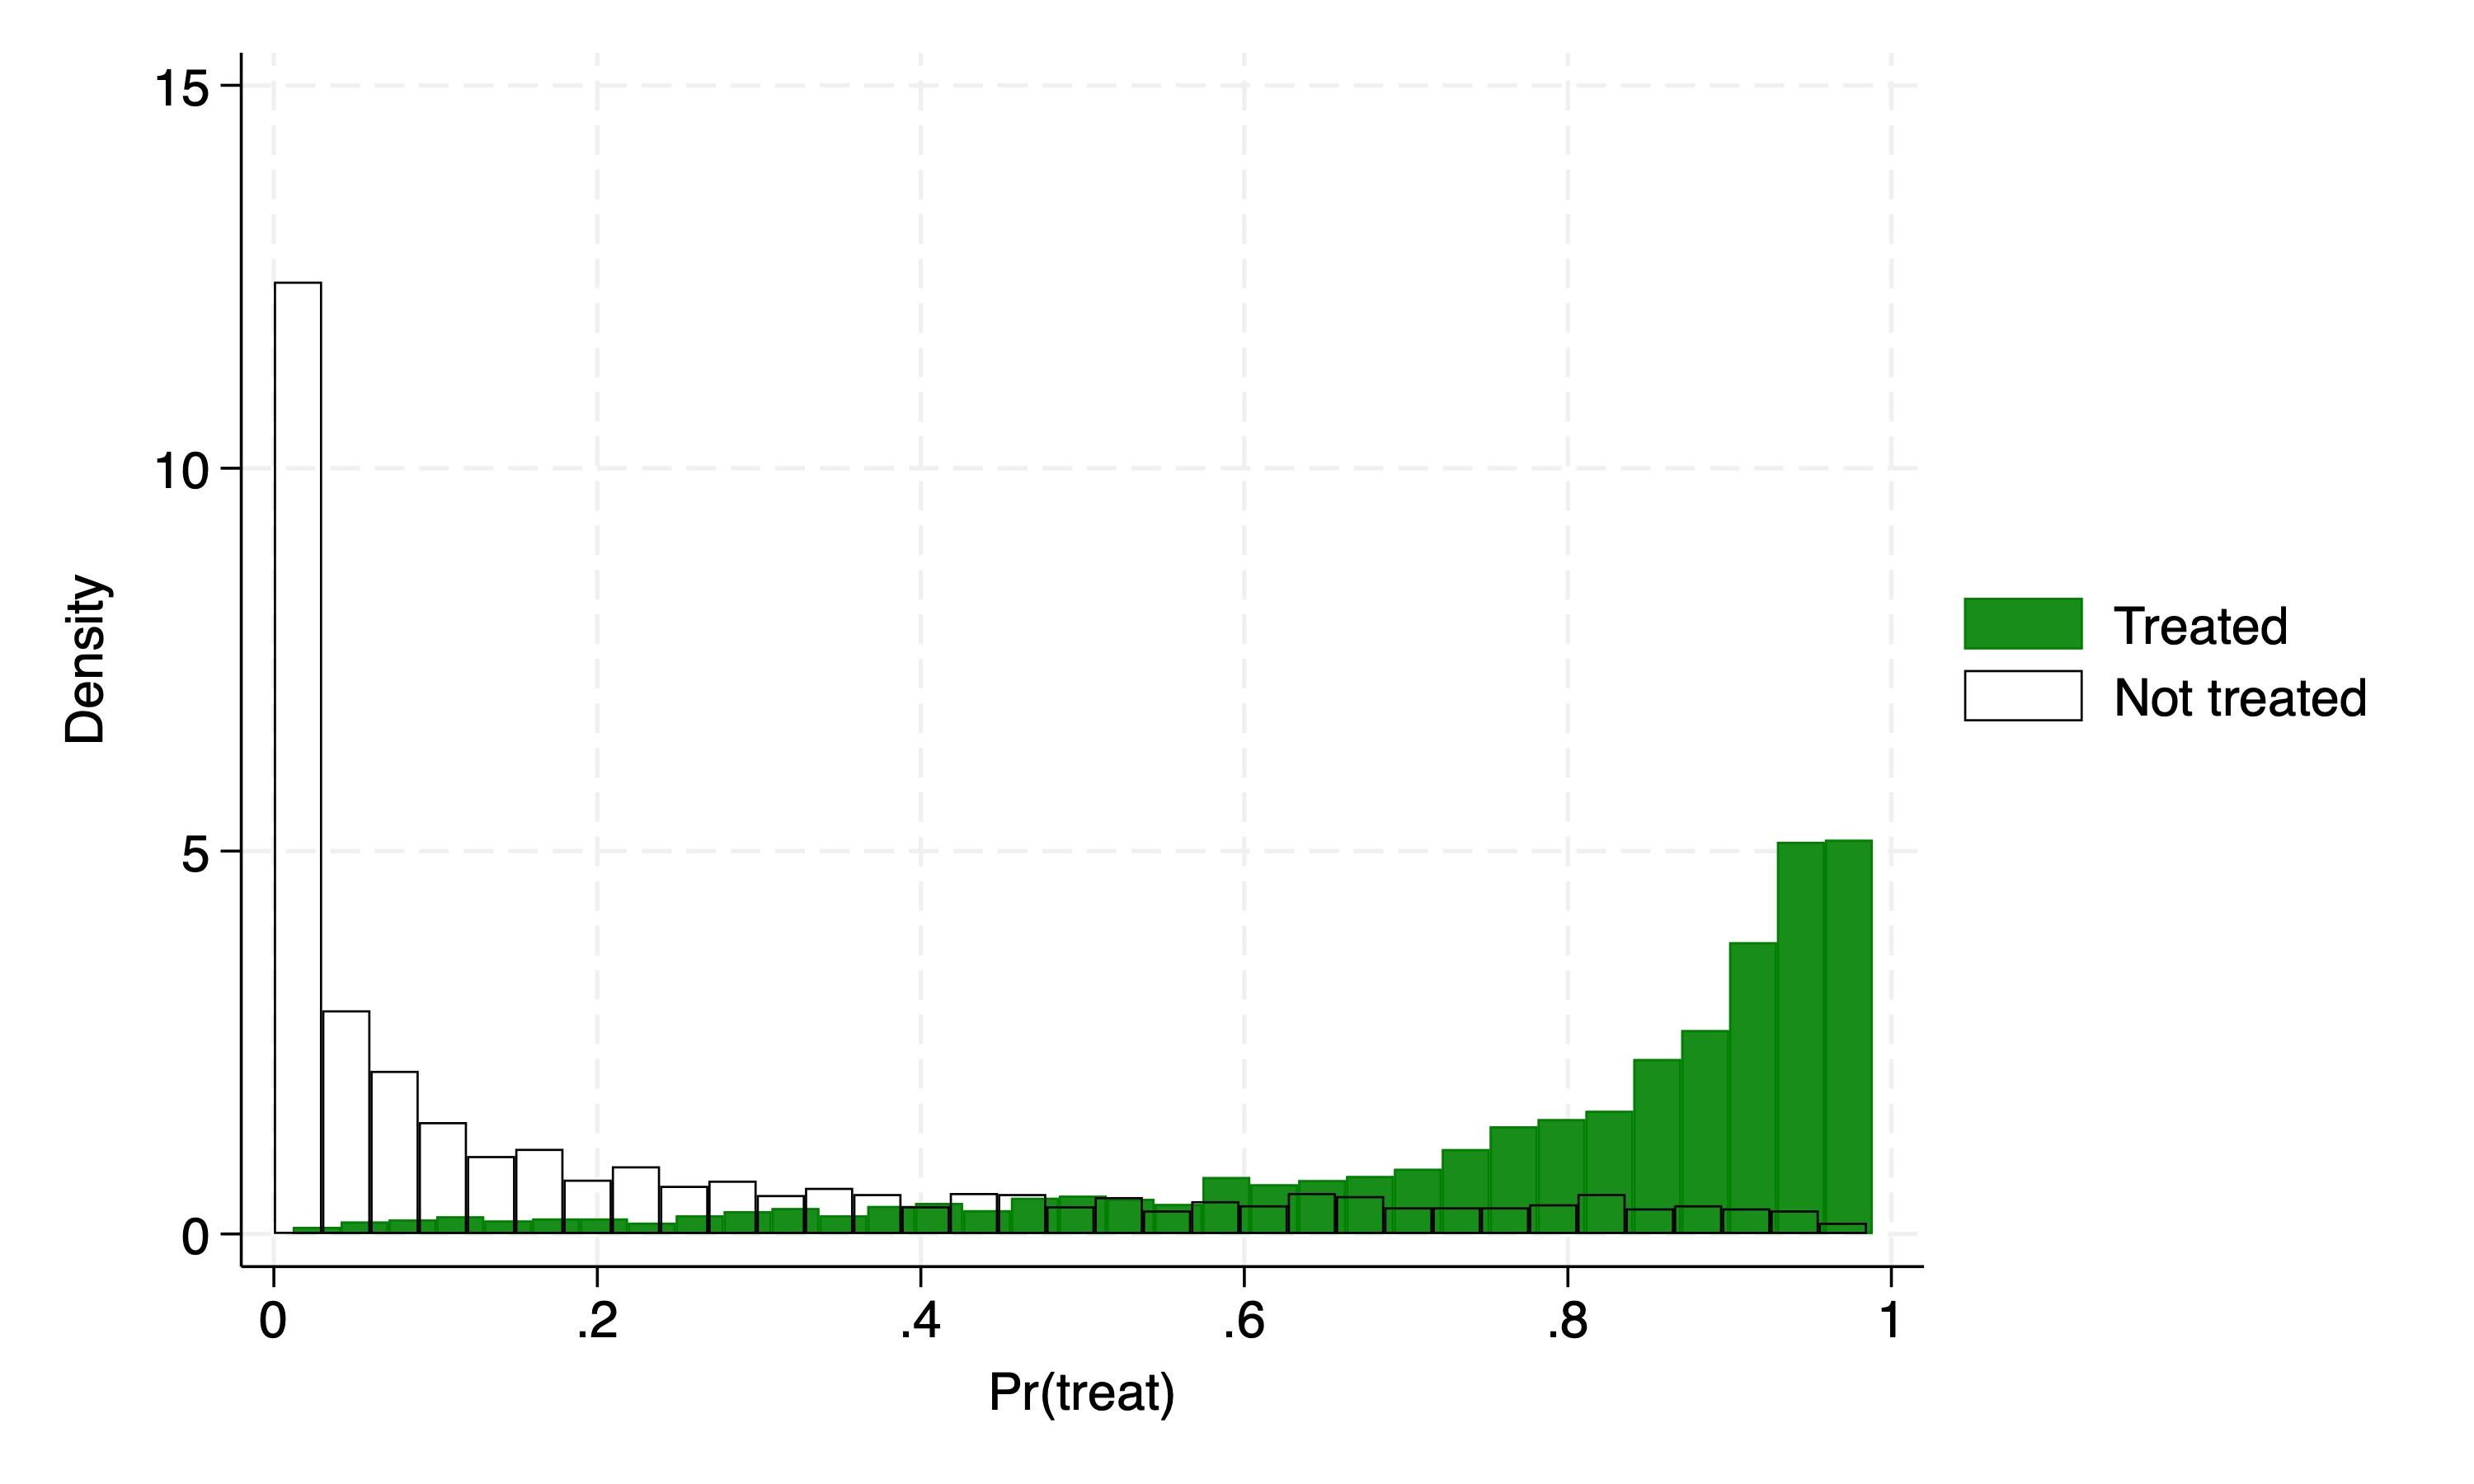
\includegraphics[scale=0.12]{./lecture_includes/pscore_overlap}
\end{figure}

\end{frame}


\begin{frame}{Concluding Remarks}

\begin{itemize}

\item Unconfoundedness implies two things: that there are no unknown confounders and that for groups of units with the same values of all confounders, treatment is assigned to units independent of either both potential outcomes (for the ATE) or just $Y^0$ (for the ATT)
\item Second assumption is also strong but testable -- common support. Can be checked with propensity score
\item If there's heterogenous treatment effects with respect to $X$, then saturated regressions as well as other methods can recover the ATT, but OLS requires linearity (but not common support), but matching and weighting require common support (but not linearity) -- the former extrapolates based on outcome modeling, but the latter interpolates

\end{itemize}

\end{frame}


\section{Synthetic control}
\subsection{Interpolation with non-negative weighting}


\begin{frame}[plain]
	\begin{figure}
	\includegraphics[scale=0.25]{./lecture_includes/currie_synth.png}
	\end{figure}
\end{frame}

\begin{frame}{What is synthetic control}
	
	\begin{itemize}
	\item Synthetic control has been called the most important innovation in causal inference of the last two decades (Athey and Imbens 2017)
	\item Originally designed for comparative case studies, but newer developments have extended it to multiple treated units as well as differential timing
	\item Continues to also be methodologically a frontier for applied econometrics, so consider this talk a starting point for you
	\end{itemize}
\end{frame}
	
\begin{frame}{What is a comparative case study}

\begin{itemize}
\item Comparative case studies compare a single unit to another unit to make causal inference
\item Single treated unit is usually a country, state, firm, etc.
\item Social scientists traditionally tackled them either qualitatively and quantitatively (more traditional economic approach)
\end{itemize}

\end{frame}


\begin{frame}{Qualitative comparative case studies}
	
	\begin{itemize}
	\item In qualitative comparative case studies, the goal might be to reason \emph{inductively} the causal effects of events or characteristics of a single unit on some outcome, oftentimes through logic and historical analysis.  
		\begin{itemize}
		\item Classic example of comparative case study approach is Alexis de Toqueville's \underline{Democracy in America} (but he is regularly comparing the US to France)
		\end{itemize}
	\item Sometimes there may not be an explicit counterfactual, or if there is, it's not principled (subjective researcher decision)
	\item Quantitative claims about causal effects are unlikely -- de Toqueville's won't claim GDP per capita fell \$500 when compared against France
	\end{itemize}
\end{frame}

\begin{frame}{Traditional quantitative comparative case studies}

\begin{itemize}
	\item Traditional quantitative comparative case studies are explicitly causal designs in that there is a treatment and control, usually involving natural experiment on a single aggregate unit
	\item Comparison focuses on the the evolution of an aggregate outcome for the unit affected by the intervention to the evolution of the same \emph{ad hoc} aggregate control group (Card 1990; Card and Krueger 1994)
	\item It'll essentially be diff-in-diff, but it may not use the event study, and the point is the choice of controls is a subset of all possible controls
\end{itemize}

\end{frame}

\begin{frame}{Pros and cons}
	
	\begin{itemize}
	\item Pros:
		\begin{itemize}
		\item Takes advantage of policy interventions that take place at an aggregate level (which is common and so this is useful)
		\item Aggregate/macro data are often available (which may be all we have)
		\end{itemize}
	\item Cons:
		\begin{itemize}
		\item Selection of control group is \emph{ad hoc} -- opens up researcher biases, even unconscious
		\item Standard errors do not reflect uncertainty about the ability of the control group to reproduce the counterfactual of interest
		\end{itemize}
	\end{itemize}
\end{frame}

\begin{frame}{Description of the Mariel Boatlift}
	
	\begin{itemize}
	\item In 1980, Fidel Castro allowed anyone to leave Cuba so long as they did in the fall from the Mariel boat dock.
	\item The Mariel Boatlift brought 100,000 Cubans to Miami which increased the Miami labor force by 7\%
	\item Card (1990) uses the Mariel Boatlift as a natural experiment to measure the effect of a sudden influx of immigrants on unemployment among less-skilled natives
	\item His question was how do inflows of immigrants affect the wages and employment of natives in local US labor markets?
	\item Individual-level data on unemployment from the Current Population Survey (CPS) for Miami and comparison cities
	\end{itemize}
\end{frame}


\begin{frame}[plain]
	\begin{figure}
	\includegraphics[scale=0.25]{./lecture_includes/boatlift2.png}
	\end{figure}
\end{frame}

\begin{frame}[plain]
	\begin{figure}
	\includegraphics[scale=0.25]{./lecture_includes/boatlift3.png}
	\end{figure}
\end{frame}

\begin{frame}[plain]
	\begin{figure}
	\includegraphics[scale=0.25]{./lecture_includes/boatlift4.png}
	\end{figure}
\end{frame}


\begin{frame}{Selecting control groups}

\begin{itemize}

\item His treatment group was low skill workers in Miami since that's where Cubans went
\item But which control group?
\item He chose Atlanta, Los Angeles, Houston, Tampa-St. Petersburg

\end{itemize}

\end{frame}



\begin{frame}{Why these four?}

	\begin{figure}
	\includegraphics[scale=0.25]{./lecture_includes/card_illr.png}
	\end{figure}

\end{frame}

\begin{frame}{Diff-in-diff}
	
	\begin{figure}
	\includegraphics[scale=0.75]{./lecture_includes/abadie_2.pdf}
	\end{figure}
\end{frame}

\begin{frame}{Parallel trends}

\begin{itemize}
\item His estimate is unbiased if the change in $Y^0$ for the comparison cities correctly approximates the unobserved $\textcolor{red}{\Delta Y^0}$ for the treatment group
\item But Card largely focused on covariates, and in a relatively casual way (``similar growth'') and does not report much
\item Black result would have been positive, too, were it not that the comparison cities growth was smaller -- uncertainty about null result being from no effect or arbitrary control group
\end{itemize}

\end{frame}


\begin{frame}{Synthetic Control}
	
	\begin{itemize}
	\item Abadie and Gardeazabal (2003) introduced synthetic control in the AER in a study of a terrorist attack in Spain (Basque) on GDP
	\item Revisited again in a 2010 JASA with Diamond and Hainmueller, two political scientists who were PhD students at Harvard (more proofs and inference)
	\item Basic idea is to use a combination of comparison units as counterfactual for a treated unit where the units are chosen according to a data driven procedure
	\end{itemize}
\end{frame}


\begin{frame}{Researcher's objectives}

\begin{itemize}
	\item Our goal here is to reproduce the counterfactual of a treated unit by finding the combination of untreated units that best resembles the treated unit \emph{before} the intervention in terms of the values of $k$ relevant covariates (predictors of the outcome of interest)
	\item Method selects \emph{weighted average of all potential comparison units} that best resembles the characteristics of the treated unit(s) - called the ``synthetic control''
\end{itemize}

\end{frame}

\begin{frame}{Synthetic control method: advantages}
	
	\begin{itemize}
	\item ``Convex hull'' means synth is a weighted average of units which means the counterfactual is a collection of comparison units that on average track the treatment group over time.
	\item Constraints on the model use non-negative weights which does not allow for extrapolation 
	\item Makes explicit the contribution of each comparison unit to the counterfactual 
	\item Formalizing the way comparison units are chosen has direct implications for inference
	\end{itemize}
\end{frame}



\begin{frame}{Notation and setup}
	
Suppose that we observe $J+1$ units in periods $1, 2, \dots, T$
		\begin{itemize}
		\item Unit ``one'' is exposed to the intervention of interest (that is, ``treated'') during periods $T_0+1, \dots, T$
		\item The remaining $J$ are an untreated reservoir of potential controls (a ``donor pool'')
		\end{itemize}	
\end{frame}



\begin{frame}{Group-time ATT with only one treated group}

Using same potential outcomes notation as we've been using, define the ATT parameter as a dynamic group-time

\begin{eqnarray*}
\delta_{1t}&=&Y_{1t}^1 - Y_{1t}^0 \\
&=& Y_{1t} - Y_{1t}^0 
\end{eqnarray*} for each post-treatment period, $t>T_0$ and $Y_{1t}$ is the outcome for unit one at time $t$. We will estimate $Y^0_{1t}$ using the $J$ units in the donor pool 

\end{frame}

\begin{frame}{Estimating W weights}
	
	\begin{itemize}
	\item Let $W=(w_2, \dots, w_{J+1})'$ with $w_j\geq 0$ for $j=2, \dots, J+1$ and $w_2+\dots+w_{j+1}=1$. Each value of $W$ represents a potential synthetic control
	\item Let $X_1$ be a $(k\times 1)$ vector of pre-intervention characteristics for the treated unit.  Similarly, let $X_0$ be a $(k\times J)$ matrix which contains the same variables for the unaffected units.
	\item The vector $W^*=(w_2^*, \dots, w_{J+1}^*)'$ is chosen to minimize $||X_1-X_0W||$, subject to our weight constraints
	\end{itemize}
\end{frame}

\begin{frame}{Donor weights and characteristic weights}
	
Abadie, et al. consider $$||X_1 - X_0W||=\sqrt{(X_1-X_0W)'V(X_1-X_0W)}$$where $X_{jm}$ is the value of the $m$-th covariates for unit $j$ and $V$ is some $(k\times k)$ symmetric and positive semidefinite matrix



\end{frame}

\begin{frame}{More on the V matrix}

Typically, $V$ is diagonal with main diagonal $v_1, \dots, v_k$.  Then, the synthetic control weights $w_2^*, \dots, w_{J+1}^*$ minimize: $$\sum_{m=1}^k v_m \bigg(X_{1m} - \sum_{j=2}^{J+1}w_jX_{jm}\bigg)^2$$ where $v_m$ is a weight that reflects the relative importance that we assign to the $m$-th variable when we measure the discrepancy between the treated unit and the synthetic controls

\end{frame}



\begin{frame}{How this works}

This method of ``minimizing pre-treatment characteristics'' is very similar to nearest neighbor matching from Abadie and Imbens (2006)

\bigskip

Let's look at it together again so you remember; it should help you understand, too, the idea of the V matrix being crucial is like switching from Euclidean distance to Maha distance in that the variables are treated differently

\bigskip

\url{https://docs.google.com/spreadsheets/d/1iro1Qzrr1eLDY_LJVzOYvnQZWmxY8JyTcDf6YcdhkwQ/edit?usp=sharing}

\end{frame}

\begin{frame}{Donor weights and characteristic weights}

\begin{itemize}
\item If all pre-treatment characteristics are treated equally, then there exists a solution to the minimization, $W^*$
\item But if pre-treatment characteristics were emphasized differently in the minimization (say one was given a weight of 0.00001), then there is a different solution, $W*'$.
\item Making a choice about $V$ (the weight on pre-treatment characteristics' importance) is unavoidable -- a non-choice is a choice as you'll just weight all characteristics the same
\end{itemize}

\end{frame}


\begin{frame}{Keeping in mind our goal - create a good synth}
	
		\begin{itemize}
		\item The synthetic control $W^*(V^*)$ is meant to reproduce the behavior of the outcome variable for the treated unit in the absence of the treatment
		\item Therefore, the $V^*$ weights directly shape $W^*$
		\end{itemize}
\end{frame}

\begin{frame}{Estimating the $V$ matrix}
	
 Choice of $v_1, \dots, v_k$ can be based on
		\begin{itemize}
		\item Assess the predictive power of the covariates using regression
		\item Subjectively assess the predictive power of each of the covariates, or calibration inspecting how different values for $v_1, \dots, v_k$ affect the discrepancies between the treated unit and the synthetic control
		\item Minimize mean square prediction error (MSPE) for the pre-treatment period (default):
			\begin{eqnarray*}
			\sum_{t=1}^{T_0} \bigg(Y_{1t} - \sum_{j=2}^J w_j^*(V^*)Y_{jt} \bigg)^2
			\end{eqnarray*}
		\end{itemize}
\end{frame}

\begin{frame}{Choosing pre-treatment characteristics}

\begin{itemize}
\item Original papers provided no guidance, and it's unclear how these characteristics connect to the factor model
\item Goal is over a long stretch pre-treatment to create the convex hull that contains the treatment group
\item Lots of early variation in what was done (including my papers), and some effort has now been made to be more principled to avoid p-hacking
\end{itemize}

\end{frame}

\begin{frame}{Cross validation}

Abadie suggests model selection using specifications guided by sample splitting into training and validation:

\begin{itemize}
		\item Divide the pre-treatment period into an initial \textbf{training} period and a subsequent \textbf{validation} period
		\item For any given $V$, calculate $W^*(V)$ in the training period.
		\item Minimize the MSPE of $W^*(V)$ in the validation period
\end{itemize}

\end{frame}


\begin{frame}{Avoiding Cherry Picking Synth}

Ferman, Pinto and Possbaum (2020) note that there are opportunities for p-hacking in model selection and recommend reporting a variety of specifications rather than just one

\begin{enumerate}
\item Use all pre-treatment lagged outcomes as your $X$ characteristics
\item Use first three-fourths
\item Use first half
\item Use all odd years
\item Use all even years
\item Use pre-treatment outcome mean
\item Use three outcome values
\end{enumerate}

\bigskip

With and without covariates, report p-values (explained later) and event study plot

\end{frame}

\begin{frame}{14 specification p-values}

	\begin{figure}
	\includegraphics[scale=0.5]{./lecture_includes/cherry_picking_1.png}
	\end{figure}

\end{frame}

\begin{frame}{14 specification event studies}

	\begin{figure}
	\includegraphics[scale=0.5]{./lecture_includes/cherry_picking_2.png}
	\end{figure}

\end{frame}


\begin{frame}{Synth identification}

\begin{itemize}
\item In diff-in-diff, the core assumption was parallel trends
\item Only needed one pretreatment period for identification but needed parallel trends starting at that period
\item Synthetic control does not use parallel trends for identification; it uses a factor model of $Y^0$
\item But you need a long pre-treatment series, not just for the event study, but for modeling the heterogeneity adequately
\end{itemize}

\end{frame}


\begin{frame}{Assumption: $Y^0$ is determined by factor model}

What about unmeasured factors affecting the outcome variables as well as heterogeneity in the effect of observed and unobserved factors?
\begin{eqnarray*}
Y_{it}^0 = \alpha_t + \theta_t Z_i + \lambda_t u_i + \varepsilon_{it}
\end{eqnarray*}where $\alpha_t$ is an unknown common factor with constant factor loadings across units, and $\lambda_t$ is a vector of unobserved common factors

\end{frame}

\begin{frame}{With some manipulation}

\begin{eqnarray*}
Y^0_{1t} - \sum^{J+1}_{j=2}w^*_jY_{jt} &=& \sum_{j=2}^{J+1} w_j^* \sum_{s=1}^{T_0} \lambda_t \bigg ( \sum_{n=1}^{T_0} \lambda_n'\lambda_n \bigg )
^{-1} \lambda_s'(\varepsilon_{js} - \varepsilon_{1s} ) \\
&& - \sum_{j=2}^{J+1} w_j^* (\varepsilon_{jt} - \varepsilon_{1t})
\end{eqnarray*}

\begin{itemize}
\item If $\sum_{t=1}^{T_0} \lambda_t' \lambda_t$ is nonsingular, then RHS will be close to zero if number of preintervention periods is ``large''  relative to size of transitory shocks 
\item Only units that are alike in observables and unobservables should produce similar trajectories of the outcome variable over extended periods of time
\item Main takeaway: you need a long pre-treatment time period to use this and the fit must be excellent
\end{itemize}


\end{frame}


\begin{frame}{Example: California's Proposition 99}
	
	\begin{itemize}
	\item In 1988, California first passed comprehensive tobacco control legislation:
		\begin{itemize}
		\item increased cigarette tax by 25 cents/pack
		\item earmarked tax revenues to health and anti-smoking budgets
		\item funded anti-smoking media campaigns
		\item spurred clean-air ordinances throughout the state
		\item produced more than \$100 million per year in anti-tobacco projects
		\end{itemize}
	\item Other states that subsequently passed control programs are excluded from donor pool of controls (AK, AZ, FL, HI, MA, MD, MI, NJ, OR, WA, DC)
	\end{itemize}
\end{frame}

\begin{frame}{Cigarette Consumption: CA and the Rest of the US}
	
	\begin{figure}
	\includegraphics[scale=0.75]{./lecture_includes/abadie_3.pdf}
	\end{figure}
\end{frame}

\begin{frame}{Cigarette Consumption: CA and synthetic CA}
	
	\begin{figure}
	\includegraphics[scale=0.75]{./lecture_includes/abadie_4.pdf}
	\end{figure}
\end{frame}

\begin{frame}{Predictor Means: Actual vs. Synthetic California}
	
	\begin{figure}
	\includegraphics[scale=0.75]{./lecture_includes/abadie_5.pdf}
	\end{figure}
\end{frame}

\begin{frame}{Smoking Gap between CA and synthetic CA}
	
	\begin{figure}
	\includegraphics[scale=0.75]{./lecture_includes/abadie_6.pdf}
	\end{figure}
\end{frame}

\begin{frame}{Inference}
	
	\begin{itemize}
	\item To assess significance, we calculate exact p-values under Fisher's sharp null using a test statistic equal to after to before ratio of RMSPE
	\item Exact p-value method
		\begin{itemize}
		\item Iteratively apply the synthetic method to each country/state in the donor pool and obtain a distribution of placebo effects
		\item Compare the gap (RMSPE) for California to the distribution of the placebo gaps. For example the post-Prop. 99 RMSPE is: 
			\begin{eqnarray*}
			RMSPE = \bigg(\frac{1}{T-T_0} \sum_{t=T_0+1}^T \bigg(Y_{1t} - \sum_{j=2}^{J+1} w_j^* Y_{jt}\bigg)^2 \bigg)^{\frac{1}{2}}
			\end{eqnarray*}and the exact p-value is the treatment unit rank divided by $J$
		\end{itemize}
	\end{itemize}
\end{frame}

\begin{frame}{Smoking Gap for CA and 38 control states}
	
	\begin{figure}
	\includegraphics[scale=0.75]{./lecture_includes/abadie_7.pdf}
	\end{figure}
\end{frame}

\begin{frame}{Smoking Gap for CA and 34 control states}
	
	\begin{figure}
	\includegraphics[scale=0.75]{./lecture_includes/abadie_8.pdf}
	\end{figure}
\end{frame}

\begin{frame}{Smoking Gap for CA and 29 control states}
	
	\begin{figure}
	\includegraphics[scale=0.75]{./lecture_includes/abadie_9.pdf}
	\end{figure}
\end{frame}

\begin{frame}{Smoking Gap for CA and 19 control states}
	
	\begin{figure}
	\includegraphics[scale=0.75]{./lecture_includes/abadie_10.pdf}
	\end{figure}
\end{frame}

\begin{frame}{Ratio Post-Prop. 99 RMSPE to Pre-Prop. 99 RMSPE}

	\begin{figure}
	\includegraphics[scale=0.75]{./lecture_includes/abadie_11.pdf}
	\end{figure}
\end{frame}




\begin{frame}{Coding exercise}
	
	\begin{itemize}
	\item The US has the highest prison population of any OECD country in the world 
	\item 2.1 million are currently incarcerated in US federal and state prisons and county jails
	\item Another 4.75 million are on parole
	\item From the early 1970s to the present, incarceration and prison admission rates quintupled in size
	\end{itemize}
\end{frame}



\begin{frame}[plain]

\begin{figure}
\includegraphics[scale=0.5]{./lecture_includes/cook2010.pdf}
\end{figure}
\end{frame}


\begin{frame}{Prison constraints}

	
	\begin{itemize}
	\item Prisons are and have been at capacity for a long time so growth in imprisonment would bite on state corrections
	\item Managing increased flows can only be solved by the following:
		\begin{itemize}
		\item Prison construction
		\item Overcrowding
		\item Paroles
		\end{itemize}
	\item Texas chooses overcrowding
	\end{itemize}
\end{frame}



\begin{frame}{Ruiz v. Estelle 1980}

	
	\begin{itemize}
		\item Class action lawsuit against TX Dept of Corrections (Estelle, warden). 
		\item TDC lost.  Lengthy period of appeals and legal decrees.  
		\item Lengthy period of time relying on paroles to manage flows
	\end{itemize}
\end{frame}

\begin{frame}[shrink=30,plain]

\begin{figure}
\includegraphics{./lecture_includes/flow_rate_figure.pdf}
\end{figure}
\end{frame}



\begin{frame}{Texas prison boom}

Governor Ann Richards (D) 1991-1995
		\begin{itemize}
		\item Operation prison capacity increased 30-35\% in 1993, 1994 and 1995. 
		\item Prison capacity increased from 55,000 in 1992 to 130,000 in 1995.  
		\item Building of new prisons (private and public)
		\end{itemize} 
\end{frame}


\begin{frame}[shrink=30,plain]

\begin{figure}
\includegraphics{./lecture_includes/tdcj.pdf}
\end{figure}
\end{frame}


\begin{frame}[shrink=30,plain]
\begin{figure}
\includegraphics{./lecture_includes/capacity_operational_texas.pdf}
\end{figure}
\end{frame}



\begin{frame}[shrink=30,plain]

\begin{figure}
\includegraphics{./lecture_includes/total_incarceration.pdf}
\end{figure}
\end{frame}

\begin{frame}[shrink=30,plain]

\begin{figure}
\includegraphics{./lecture_includes/synth_placebo_totalincarceration1993.pdf}
\end{figure}
\end{frame}





\subsection{Extrapolation with Conservative Negative Weighting}

\begin{frame}{Synth Opponents}

\begin{itemize}

\item Synthetic control has opponents
\item One criticism is people will say the weights are implausible
\item But that's because they have their own ``mental synth'' model that tells them what weights should or shouldn't be
\item Tell story about conference where Abadie presented Germany paper
\item Synth tells you the weights; OLS you have to calculate them and no one does

\end{itemize}

\end{frame}

\begin{frame}{Regression vs synth weights}
	\begin{figure}
	\includegraphics[scale=0.4]{./lecture_includes/abadie2015_table1.png}
	\end{figure}
\end{frame}



\begin{frame}{Comment about Negative Weights}

\begin{itemize}

\item Matching principles favor non-negative weighting because similar groups are best comparisons for a treated group, not dissimilar ones
\item But what if you're Michael Jordan and wanting to know his synthetic control -- can you find a positively weighted average group of players that approximate him over his career if he is an outlier?
\item You cannot with non-negative weights, but you could with negative weights

\end{itemize}

\end{frame}

\begin{frame}{Comment about Negative Weights}

\begin{itemize}

\item Negative weights would mean finding a truly horrible player and then negatively weighting him 
\item But if you are never willing to negatively weight, some questions you cannot answer
\item Non-negative weights by Abadie are not the best fit -- they are the best fit given you can't negatively weight
\item Perhaps there is a compromise -- the least worst negative weighting, or ``augmented synthetic control''

\end{itemize}

\end{frame}


\begin{frame}{Non-negative weighting and poor fit}

\begin{quote}
``The applicability of the [ADH2010] method requires a sizable number of pre-intervention periods. The reason is that the credibility of a synthetic control depends upon how well it tracks the treated unit’s characteristics and outcomes over an extended period of time prior to the treatment. \textbf{We do not recommend using this method when the pretreatment fit is poor or the number of pretreatment periods is small}. A sizable number of post-intervention periods may also be required in cases when the effect of the intervention emerges gradually after the intervention or changes over time.'' (my emphasis, Abadie, et al. 2015)
\end{quote}

\end{frame}


\begin{frame}{Introducing Augmented Synthetic Control}
\begin{itemize}
\item Synthetic control has built in constraints forcing weights to be non-negative
\item Convex hull constraint ensures that synth is a feasible counterfactual in that it is formed by a combination of control units similar on pre-intervention characteristics
\item Improves the validity of the estimated effect as there exists interpolated comparison group; similar to common support concept
\item But, the convex hull constraint reduces extrapolation bias from comparing dissimilar units, but at the cost of failing to find matches at all
\end{itemize}

\end{frame}



\begin{frame}{What is augmented synthetic control?}

\begin{itemize}
\item Eli Ben-Michael, Avi Feller and Jesse Rothstein present a modification to ADH in which they allow for negative weights, but only minimally so
\item This model will ``augment'' the original synthetic control model by adjusting for pre-treatment imbalance using doubly robust bias adjustment 
\item Augmentation is conservative; it uses \textbf{penalized ridge regression} but with constraints such that the negative weighting is only to the convex hull, not to the center of the convex hull
\end{itemize}

\end{frame}




\begin{frame}{Optimal weights}

Synth minimizes the following norm:

\begin{eqnarray*}
\textrm{min}_w = || V_X^{1/2} (X_1 - X_0'w) ||_2^2 + \psi \sum_{D_j=0}f(w_j)\\
\textrm{s.t. }\sum_{j=2}^N w_{j} =1 \textrm{ and } w_j \geq 0
\end{eqnarray*}

$Y_0'w*$ (i.e., optimally weighted donor pool) is the unit 1 ``synthetic control'' .  We are hoping that $\widehat{Y}_1^0$ with $Y_0' {w}^{*}$ based on ``perfect fit'' pre-treatment


\end{frame}


\begin{frame}{Slight change in synth notation}

\begin{itemize}
\item Assume that our outcome, $Y_{jt}$, follows a factor model where $m(.)$ are pre-treatment outcomes: $$ Y_{jt}^0 = m_{jt} + \varepsilon_{jt}$$
\item Since $\widehat{m(.)}$ estimates the post-treatment outcome, let's view it as estimated bias, analogous to bias correction for inexact matching from earlier (Abadie and Imbens 2011)
\end{itemize}

\end{frame}



\begin{frame}{Bias correction}

 $$ Y_{jt}^0 = m_{jt} + \varepsilon_{jt}$$

\begin{itemize}
\item When the weights achieve exact balance, the bias of synthetic control decreases with $T$
\item The intuition is that for a large $T$ ($T$ not transitory shocks), you achieve balance by balancing the latent parameter on the unobserved heterogeneity in our factor model
\end{itemize}

\end{frame}


\begin{frame}{Treatment and control units}

	\begin{figure}
	\includegraphics[scale=0.07]{./lecture_includes/convexhull_1.png}
	\end{figure}

\end{frame}

\begin{frame}{Convex hull -- ideal for synth}

	\begin{figure}
	\includegraphics[scale=0.07]{./lecture_includes/convexhull_2.png}
	\end{figure}

\end{frame}

\begin{frame}{Outside the convex hull bc of dimensionality}

	\begin{figure}
	\includegraphics[scale=0.07]{./lecture_includes/convexhull_3.png}
	\end{figure}

\end{frame}

\begin{frame}{Outside the convex hull bc of dimensionality}

	\begin{figure}
	\includegraphics[scale=0.07]{./lecture_includes/convexhull_4.png}
	\end{figure}

\end{frame}


\begin{frame}{Reweighting Original Synth}
 
\begin{itemize}
\item Adjust the synthetic control approach to adjust for poor fit pre-treatment.
\item We don't estimate new donor pool weights -- we estimate the bias and then reweight the original weights, which introduces the negative weighting
\item The augmented synthetic control estimator for $Y_{jt}^0$ is on the next slide, but the bias adjustment is very similar to Abadie and Imbens (2011) earlier (i.e., it subtracts out linearly)
\end{itemize}


\end{frame}




\begin{frame}{Setup of the estimator}

Let's adjust synthetic control for this bias.  First we'll apply the \textbf{bias correction}.  Then we'll do the doubly robust augmented \textbf{inverse probability weighting}. Let $Y_1^{aug,0}$ be the augmented potential outcome

\begin{eqnarray*}
Y_1^{aug,0} &=& \sum_{D_j=0} \widehat{w}_j^{synth} Y_{j} + \widehat{m}(X_1) - \sum_{D_j=0} \widehat{w}_j \widehat{m}(X_j) \\
&=& \widehat{m}(X_1) + \sum_{D_j=0} \widehat{w_j}(Y_j - \widehat{m}(X_j))
\end{eqnarray*}

\end{frame}


\begin{frame}{Interpreting line 1}

\begin{eqnarray*}
Y_1^{aug,0} &=& \sum_{D_j=0} \widehat{w}_j^{synth} Y_{jT} + \bigg (\widehat{m}_{1T} - \sum_{D_j=0} \widehat{w}_j^{synth}\widehat{m}_{jT} \bigg ) \\
&=& \widehat{m}_{1T} + \sum_{D_j=0} \widehat{w}_j^{synth} (Y_{jT} - \widehat{m}_{jT})
\end{eqnarray*}

(1) Note how in the first line the traditional synthetic control weighted outcomes are corrected by the imbalance in a particular function of the pre-treatment outcomes $\widehat{m}$. 
\end{frame}




\begin{frame}{Interpreting line 1}

\begin{eqnarray*}
Y_1^{aug,0}  &=& \sum_{D_j=0} \widehat{w}_j^{synth} Y_{jT} + \bigg (\widehat{m}_{1T} - \sum_{D_j=0} \widehat{w}_j^{synth}\widehat{m}_{jT} \bigg ) \\
&=& \widehat{m}_{1T} + \sum_{D_j=0} \widehat{w}_j^{synth} (Y_{jT} - \widehat{m}_{jT})
\end{eqnarray*}

(1) Since $\widehat{m}$ estimates the post-treatment outcome, we can view this as an estimate of the bias due to imbalance, which is similar to how you address imbalance in matching with a bias correction formula (Abadie and Imbens 2011). 

\end{frame}





\begin{frame}{Interpreting line 1}
\begin{eqnarray*}
Y_1^{aug,0}  &=& \sum_{D_j=0} \widehat{w}_j^{synth} Y_{jT} + \bigg (\widehat{m}_{1T} - \sum_{D_j=0} \widehat{w}_j^{synth}\widehat{m}_{jT} \bigg ) \\
&=& \widehat{m}_{1T} + \sum_{D_j=0} \widehat{w}_j^{synth} (Y_{jT} - \widehat{m}_{jT})
\end{eqnarray*}

(1) So if the bias is small, then synthetic control and augmented synthetic control will be similar because that interior term will be zero.

\end{frame}

\begin{frame}{Interpreting line 2}

\begin{eqnarray*}
Y_1^{aug,0}  &=& \sum_{D_j=0} \widehat{w}_j^{synth} Y_{jT} + \bigg (\widehat{m}_{1T} - \sum_{D_j=0} \widehat{w}_j^{synth}\widehat{m}_{jT} \bigg ) \\
&=& \widehat{m}_{1T} + \sum_{D_j=0} \widehat{w}_j^{synth} (Y_{jT} - \widehat{m}_{jT})
\end{eqnarray*}

(2) The second equation is equivalent to a double robust estimation which begins with an outcome model but then re-weights it to balance residuals.


\end{frame}



\begin{frame}{Interpreting line 2}

\begin{eqnarray*}
Y_1^{aug,0}  &=& \sum_{D_j=0} \widehat{w}_j^{synth} Y_{jT} + \bigg (\widehat{m}_{1T} - \sum_{D_j=0} \widehat{w}_j^{synth}\widehat{m}_{jT} \bigg ) \\
&=& \widehat{m}_{1T} + \sum_{D_j=0} \widehat{w}_j^{synth} (Y_{jT} - \widehat{m}_{jT})
\end{eqnarray*}

(2) The second equation has a connection to inverse probability weighting (they show this in an appendix)


\end{frame}
\begin{frame}{Ridge Augmented SCM}

\begin{eqnarray*}
\textrm{arg min}_{\eta_0,\eta} \frac{1}{2} \sum_{D_j=0} (Y_j - (\eta_0 + X_j'\eta))^2 + \lambda^{ridge} || \eta ||_2^2
\end{eqnarray*}Here we estimate $\widehat{m}(X_j)$ with ridge regularized linear model and penalty hyper parameter $\lambda^{ridge}$. We then adjust for imbalance using the $\widehat{\eta}^{ridge}$ parameter as a weight on the outcome model itself. 

\end{frame}





\begin{frame}{Go back to that weighting but use the ridge parameters}

\begin{eqnarray*}
Y_1^{aug,0} &=& \sum_{D_j=0} \widehat{w}_j^{synth} Y_{j} + \bigg ( X_1 - \sum_{D_j=0} \widehat{w}_j^{synth} X_j \bigg ) \widehat{\eta}^{ridge} \\
&=& \sum_{D_j=0} \widehat{w}_j^{aug}Y_j
\end{eqnarray*}What you're trying to do is adjust with the $\widehat{w}_j^{aug}$ weights to improve balance.  

\end{frame}


\begin{frame}{The ridge weights are key to the augmentation}

\begin{eqnarray*}
\widehat{w}_j^{aug} = \widehat{w}_j^{synth} + (X_j - X_0' \widehat{w}_j^{synth}) ' (X_0'X_0 + \lambda I_{T_0})^{-1}X_i
\end{eqnarray*}

The second term is adjusting the original synthetic control weights, $w_j^{synth}$ for better balance. Again remember -- we are trying to address the bias due to imbalance. You can achieve better balance, but at higher variance and can introduce negative weights. 

\end{frame}



\begin{frame}{Ridge will allow negative weights via extrapolation}

\begin{eqnarray*}
\widehat{w}_j^{aug} = \widehat{w}_j^{synth} + (X_j - X_0' \widehat{w}_j^{synth}) ' (X_0'X_0 + \lambda I_{T_0})^{-1}X_i
\end{eqnarray*}

Relaxing the constraint from synth that weights be non-negative, as non-negative weights prohibit extrapolation. But we don't have synthetic control on the simplex, so we \emph{must} extrapolate, otherwise synth will be biased.

\end{frame}



\begin{frame}{Summarizing and some comments}

\begin{itemize}
\item When the treated unit lies in the convex hull of the control units so that the synth weights exactly balance lagged outcomes, then SCM and Ridge ASCM are the same
\item When synth weights do not achieve exact balance, Ridge ASCM will use negative weights to extrapolate from the convex hull to the control units
\item The amount of extrapolation will be determined by how much imbalance we're talking about and the estimated hyperparameter $\widehat{\lambda}^{ridge}$
\item When synth has good pre-treatment fit or when $\lambda^{ridge}$ is large, then adjustment will be small and the augmented weights will be close to the SCM weights
\end{itemize}

\end{frame}



\begin{frame}{Intuition}

Ridge begins at the center of control units, while Ridge ASCM begins at the synth solution. Both move towards an exact fit solution as the hyperparameter is reduced. It is possible to achieve the same level of balance with non-negative weights.  Both ridge and Ridge ASCM extrapolate from the support of the data to improve pre-treatment fit relative to synth alone. Let's look at a picture!


\end{frame}



\begin{frame}[plain]

	\begin{figure}
	\includegraphics[scale=0.5]{./lecture_includes/aug_1.png}
	\end{figure}
	
\end{frame}	


\begin{frame}{Conformal Inference}

Whereas Abadie, et al. used Fisher sharp null and randomization inference, newer synth models will conduct inference based on conformal inference  (Chernozhukov et al. 2019)

\bigskip

We can get 95\% point-wide confidence intervals, or use a jackknife method by Barber et al (2019) 

\end{frame}


\begin{frame}{Comparing four synth models}

\begin{itemize}
\item Non-negative weighted synth vs three augmented synth models (no covariates, covariates, residualized covariates)
\item Augmenting synth with a ridge outcome regression reduces bias relative to synth alone in application (but note at the cost of negative weights)
\item This underscores the importance of the recommendation Abadie, et al. (2015) make which is that synth should be used in settings with excellent pre-treatment fit
\end{itemize}

\end{frame}

\imageframe{./lecture_includes/aug_5.png}

\imageframe{./lecture_includes/aug_6.png}

\begin{frame}{Couple of minor points}

\begin{itemize}
\item Hyper parameter chosen using cross validation
\item This can be extended to auxiliary covariates as opposed to just lagged outcomes (section 6)
\end{itemize}

\end{frame}



\begin{frame}{Concluding remarks}

\begin{itemize}
\item Non-negative weights preclude extrapolation forcing us to use similar groups as synthetic controls, but it may also make the project impossible if our treatment group is too ``unique'' 
\item Ridge regression augmentation is like the ``least worst'' way to do negative weighting -- it's bias adjustment with weights estimated using ridge that shifts the convex hull the minimum distance needed to balance through negative weights
\item Augmented synth will dominate synth in those instances by extrapolating outside the convex hull
\end{itemize}

\end{frame}

\begin{frame}{More synthetic control}

\begin{itemize}

\item Synthetic control remains an active area in econometrics and Athey and Imbens have contributed two new ones (matrix completion with nuclear norm regularization and synthetic difference-in-differences)
\item MCNN can handle panel data and a variety of designs including staggered adoption and uses imputation based on vertical and horizontal regressions in pre-treatment period
\item Synthetic control continues to evolve in such a way that it appears to be encroaching on difference-in-differences, but it's important to know that synth needs a longer pre-treatment time series than diff-in-diff which we will look at now
\end{itemize}

\end{frame}


\section{Difference-in-differences}


\subsection{Four averages and three subtractions}

\begin{frame}{Types of evidence}

Difference-in-differences does not rely on covariates or randomization, so the types of evidence needed shifts and can be somewhat more involved -- the underlying estimator is itself simple, but the evidence is not

\begin{itemize}
\item You are building a case, the prosecutor before a judge and jury, always in battle with the defense attorney
\item You are producing evidence, not proofs, and that evidence has particular broadly defined forms that can help you on the front end
\item Your goal in my humble opinion should be reasonable and theoretically relevant falsifications with particular kinds of data visualization, starting with the event study
\end{itemize}

\end{frame}




\begin{frame}{What is difference-in-differences (DiD)}

\begin{itemize}
\item DiD is a very old, relatively straightforward, intuitive research design
\item A group of units are assigned some treatment and then compared to a group of units that weren't
\item One of the most widely used quasi-experimental methods in economics and increasingly in industry
\item Mostly associated with ``big shocks'' happening in space over time
\end{itemize}


\begin{quote}
``A good way to do econometrics is to look for good natural experiments and use statistical methods that can tidy up the confounding factors that nature has not controlled for us.'' -- Daniel McFadden (Nobel Laureate recipient with Heckman 2002)
\end{quote}

\end{frame}


\begin{frame}

	\begin{figure}
	\caption{Currie, et al. (2020)}
	\includegraphics[scale=0.25]{./lecture_includes/currie_did.png}
	\end{figure}


\end{frame}


\begin{frame}{Difference-in-differences}

\begin{table}\centering
		\caption{Treatment and Control, Before and After}
		\begin{center}
		\begin{tabular}{lll|lc}
		\toprule
		\multicolumn{1}{l}{\textbf{Companies}}&
		\multicolumn{1}{c}{\textbf{Time}}&
		\multicolumn{1}{c}{\textbf{Outcome}}&
		\multicolumn{1}{c}{$D_1$}&
		\multicolumn{1}{c}{$D_2$}\\
		\midrule
		Treatment & Before & $Y=L$ \\
		& After & $Y=L + T_L + D$ & $T_L+D$\\
		\midrule
		& & & & $D$ \\
		\midrule
		Comparison & Before & $Y=SV$ \\
		& After & $Y=SV + T_{SV}$ & $T_{SV}$\\
		\bottomrule
		\end{tabular}
		\end{center}
	\end{table}

\begin{eqnarray*}
\widehat{\delta}_{did} = D + (T_L - T_{SV})
\end{eqnarray*}This simple method yields an unbiased estimate of D if $T_{SV} = \textcolor{red}{T_L}$

\end{frame}


\begin{frame}{Relationship to OLS}

\begin{itemize}
\item Orley Ashenfelter graduated from Princeton in the 1970s, takes a job in Washington DC and begins studying ``job trainings programs''
\item Empirical crisis in empirical macro and empirical labor back in the 1970s -- Orley, David Card, Bob Lalonde, Alan Krueger at Princeton all helped bring attention to it and began pushing for solutions, one of which was RCTs in labor but also diff-in-diff as well as better instruments
\item Listen to Orley explain the connection he made between twoway fixed effects and difference-in-differences; it was born out of a need to explain OLS to an American bureaucrat

\end{itemize}

\url{https://youtu.be/WnB3EJ8K7lg?t=126}

\end{frame}


\begin{frame}{Equivalence}
$$Y_{ist} = \alpha_0 + \alpha_1 Treat_{is} + \alpha_2 Post_{t} + \textcolor{blue}{\delta} (Treat_{is} \times Post_t) + \varepsilon_{ist} $$

\bigskip

$$\widehat{\textcolor{blue}{\delta}} = \bigg ( \overline{y}_k^{post(k)} - \overline{y}_k^{pre(k)} \bigg ) - \bigg ( \overline{y}_U^{post(k)} - \overline{y}_U^{pre(k)} \bigg ) $$

\begin{itemize}
\item Orley claims that the OLS estimator of $\delta$ and the ``four averages and three subtractions'' are the same thing numerically
\item And they are -- they are numerically \emph{identical}
\item And under a particular assumption, they are also unbiased estimates of an aggregate causal parameter
\item But to see this we need new notation -- potential outcomes
\end{itemize}

\end{frame}




\begin{frame}{DiD equation}

Orley's ``four averages and three subtractions''

\begin{eqnarray*}
\widehat{\delta} = \bigg ( E[Y_k|Post] - E[Y_k|Pre] \bigg ) - \bigg ( E[Y_U | Post ] - E[ Y_U | Pre] \bigg) \\
\end{eqnarray*}$k$ are the people in the job training program, $U$ are the untreated people not in the program, $Post$ is after the trainees took the class, $Pre$ is the period just before they took the class, and $E[y]$ is mean earnings. 

\bigskip

Does $\widehat{\delta}$ equal the ATT?  If so when? If not why not?

\end{frame}



\begin{frame}{Potential outcomes and the switching equation}

\begin{eqnarray*}
\widehat{\delta} &=& \bigg ( \underbrace{E[Y^1_k|Post] - E[Y^0_k|Pre] \bigg ) - \bigg ( E[Y^0_U | Post ] - E[ Y^0_U | Pre]}_{\mathclap{\text{Switching equation}}} \bigg)  \\
&&+ \underbrace{\textcolor{red}{E[Y_k^0 |Post] - E[Y^0_k | Post]}}_{\mathclap{\text{Adding zero}}} 
\end{eqnarray*}

\end{frame}

\begin{frame}{Parallel trends bias}

\begin{eqnarray*}
\widehat{\delta} &=& \underbrace{E[Y^1_k | Post] - \textcolor{red}{E[Y^0_k | Post]}}_{\mathclap{\text{ATT}}} \\
&& + \bigg [  \underbrace{\textcolor{red}{E[Y^0_k | Post]} - E[Y^0_k | Pre] \bigg ] - \bigg [ E[Y^0_U | Post] - E[Y_U^0 | Pre] }_{\mathclap{\text{Non-parallel trends bias in 2x2 case}}} \bigg ]
\end{eqnarray*}


\end{frame}

\begin{frame}{Identification through parallel trends}
	

	\begin{block}{Parallel trends}
	Assume two groups, treated and comparison group, then we define parallel trends as:	 $$\textcolor{red}{E(}\textcolor{red}{\Delta Y^0_k)} = E(\Delta Y^0_U)$$
	\end{block}

\textbf{In words}: ``The \textcolor{red}{evolution of earnings for our trainees \emph{had they not trained}} is the same as the evolution of mean earnings for non-trainees''.  

\bigskip

It's in \textcolor{red}{red} because parallel trends is untestable and critically important to estimation of the ATT using any method, OLS or ``four averages and three subtractions''


	
\end{frame}


\begin{frame}{What is parallel trends}

\begin{itemize}
\item Parallel trends assumes away the selection bias associated with comparisons
\item The assumption is thought to be more plausible than simply assuming simple comparisons held equal $E[Y^0|D=0]=E[Y^0|D=1]$
\item But it is still a strong assumption, and differs from the assumptions have in the RCT which though also untestable, is nearly guaranteed by randomization
\item Most of the hard part of the work involves the old fashioned detective work and the work of making good arguments with good exhibits (tables and figures)
\end{itemize}

\end{frame}



\begin{frame}{Understanding parallel trends through worksheets}

Before we move into regression, let's go through a simple exercise to really pin down these core ideas with simple calculations

\bigskip 

\url{https://docs.google.com/spreadsheets/d/1onabpc14JdrGo6NFv0zCWo-nuWDLLV2L1qNogDT9SBw/edit?usp=sharing}

\end{frame}



\begin{frame}{OLS Specification}
	
	\begin{itemize}
	\item Simple DiD equation will identify ATT under parallel trends
	\item But so will a particular OLS specification (two groups and no covariates)
	\item OLS was historically preferred because
		\begin{itemize}
		\item OLS estimates the ATT under parallel trends
		\item Easy to calculate the standard errors
		\item Easy to include multiple periods
		\end{itemize}
	\item People liked it also because of differential timing, continuous treatments and covariates, but those are more complex so we address them later
	\end{itemize}
\end{frame}

\begin{frame}{Minimum wages}

\begin{itemize}
\item Card and Krueger (1994) have a famous study estimating causal effect (ATT) of minimum wages on employment
\item Exploited a policy change in New Jersey between February and November in mid-1990s where minimum wage was increased, but neighbor PA did not
\item Using DiD, they do not find a negative effect of the minimum wage on employment which is part of its legacy today, but I mainly present it to illustrate the history and the design principles
\end{itemize}

\end{frame}

\begin{frame}
	\begin{figure}
	\includegraphics[scale=0.5]{./lecture_includes/minwage_whore}
	\end{figure}
\end{frame}

\begin{frame}{Card on that study}

\begin{quote}
``I’ve subsequently stayed away from the minimum wage literature for a number of reasons. First, it cost me a lot of friends. People that I had known for many years, for instance, some of the ones I met at my first job at the University of Chicago, became very angry or disappointed. They thought that in publishing our work we were being traitors to the cause of economics as a whole.''
\end{quote}

\bigskip

But let's listen to Orley's opinion about the paper's controversy at the time.  \url{https://youtu.be/MOtbuRX4eyQ?t=1882}

\end{frame}


\begin{frame}{OLS specification of the DiD equation}
	
	\begin{itemize}
	\item The correctly specified OLS regression is an interaction with time and group fixed effects:$$Y_{its} = \alpha + \gamma NJ_s + \lambda d_t + \delta (NJ \times d)_{st} + \varepsilon_{its}$$
		\begin{itemize}
		\item NJ is a dummy equal to 1 if the observation is from NJ
		\item d is a dummy equal to 1 if the observation is from November (the post period)
		\end{itemize}
	\item This equation takes the following values
		\begin{itemize}
		\item PA Pre: $\alpha$
		\item PA Post: $\alpha + \lambda$
		\item NJ Pre: $\alpha + \gamma$
		\item NJ Post: $\alpha + \gamma + \lambda + \delta$
		\end{itemize}
	\item DiD equation: (NJ Post - NJ Pre) - (PA Post - PA Pre) $= \delta$
	\end{itemize}
\end{frame}




\begin{frame}[plain]
	$$Y_{ist} = \alpha + \gamma NJ_s + \lambda d_t + \delta(NJ\times d)_{st} + \varepsilon_{ist}$$
	\begin{figure}
	\includegraphics[scale=0.90]{./lecture_includes/waldinger_dd_5.pdf}
	\end{figure}
\end{frame}


\begin{frame}[plain]
	$$Y_{ist} = \alpha + \gamma NJ_s + \lambda d_t + \delta(NJ\times d)_{st} + \varepsilon_{ist}$$
	\begin{figure}
	\includegraphics[scale=0.90]{./lecture_includes/waldinger_dd_5.pdf}
	\end{figure}

Notice how OLS is ``imputing'' $E[Y^0|D=1,Post]$ for the treatment group in the post period? It is only ``correct'', though, if parallel trends is a good approximation

\end{frame}


\begin{frame}{Inference}
	
	\begin{itemize}
	\item  Bertrand, Duflo and Mullainathan (2004) show that conventional standard errors will often severely understate the standard deviation of the estimators
	\item Standard errors are biased downward (i.e., too small, over reject)
	\item They proposed three solutions, but most only use one of them (clustering)
	\end{itemize}
\end{frame}


\begin{frame}{Inference}
	
		\begin{enumerate}
		\item[1 ] Block bootstrapping standard errors (if you analyze states the block should be the states and you would sample whole states with replacement for bootstrapping)
		\item[2 ] Clustering standard errors at the group level (in Stata one would simply add \texttt{, cluster(state)} to the regression equation if one analyzes state level variation)
		\end{enumerate}

\bigskip

Most people will simply cluster, but there are issues if you have too few clusters. They mention a third way but it's only a curiosity.
		
\end{frame}


\begin{frame}{Main DiD assumptions}

There are actually three DiD assumptions in the basic design, but you usually only hear about the first:

\bigskip

\begin{enumerate}
\item Parallel trends -- concerns changes in $Y^0$, one of which is a fictional change because the post treatment $Y^0$ doesn't exist for the treated
\item No anticipation (next slide)
\item SUTVA (slide after next)
\end{enumerate}

\end{frame}

\begin{frame}{No Anticipation}

\begin{itemize}
\item No anticipation means that the treatment effect happens only at the time that the treatment occurs or after, but not before
	\begin{itemize}
	\item \textbf{Example 1}: Tomorrow I win the lottery, but don't get paid yet. I decide to buy a new house today. That violates NA
	\item \textbf{Example 2}: Next year, a state lets you drive without a driver license and you know it. But you can't drive without a driver license today.  This satisfies NA.
	\end{itemize}
\item Requires that baseline in pre-period is untreated $Y=Y^0$ for treated group
\item Crucial for DiD equation collapsing to ATT plus PT bias
\end{itemize}

\end{frame}

\begin{frame}{SUTVA}

\begin{itemize}
\item Stable Unit Treatment Value Assumption (Imbens and Rubin 2015) focuses on what happens when in our analysis we are combining units (versus defining treatment effects)
	\begin{enumerate}
	\item \textbf{No Interference}: a treated unit cannot impact a control unit such that their potential outcomes change (unstable treatment value)
	\item \textbf{No hidden variation in treatment}: When units are indexed to receive a treatment, their dose is the same as someone else with that same index
	\item \textbf{Scale}: If scaling causes interference or changes inputs in production process, then \#1 or \#2 are violated
	\end{enumerate}
\item Shifts from defining treatment effects to estimating them, which means being careful about who is the control group, how you define treatments and what questions can and cannot be answered with this method
\item Again, we need our control group to be untreated $(Y=Y^0)$ otherwise DiD doesn't equal ATT + PT
\end{itemize}

\end{frame}







\begin{frame}{Violating parallel trends exercise}

\begin{itemize}
\item Parallel trends are needed so we can impute the missing $E[Y^0|D=1]$ with $E[Y^0|D=0]$ either explicitly or implicitly
\item Which means if parallel trends isn't true, then the imputation isn't correct and therefore estimates are biased
\item To illustrate this, let's go through the document again -- this time to tab 2
\end{itemize}

\url{https://docs.google.com/spreadsheets/d/1onabpc14JdrGo6NFv0zCWo-nuWDLLV2L1qNogDT9SBw/edit?usp=sharing}

\end{frame}

\begin{frame}{Event studies and pre-trends}

\begin{itemize}
	\item Parallel trends involves, $Y^0$, specifically $\Delta E[\textcolor{red}{Y^0}|D=1] = \Delta E[Y^0|D=0]$ 
		\begin{itemize}
		\item  Notice that parallel trends is about $Y^0$ in other words, not $Y^1$
		\end{itemize}
	\item We cannot verify the \textcolor{red}{red} term, because the change is post-treatment and thus counterfactual (fictional)
	\item But there are other non-red $\Delta E[Y^0|D=1]$ that aren't fictional which we can investigate, but where?
\end{itemize}

\bigskip

``Pre-trends'' are also $\Delta E[Y^0|D=1]$, just non-fictional in nature

\bigskip

Testing for parallel pre-trends is a type of falsification for selection bias

\end{frame}

\begin{frame}{Intuition behind event studies}
	
	\begin{itemize}
	\item Checking pre-trends is \textbf{not} a test for parallel trends as there is no formal test for parallel trends
	\item It's akin to finding a smoking gun -- maybe someone planted it, but dismiss it is irresponsible
	\item Do not overweight nor underweight parallel pre-trends
	\item Even if pre-trends are the same one still has to worry about other policies changing at the same time (omitted variable bias is a parallel trends violation)

\end{itemize}

\end{frame}


\begin{frame}{Event study regression}
	
	\begin{itemize}
	\item Event studies have a simple OLS specification with only one treatment group and one never-treated group $$Y_{its} = \alpha +  \sum_{\tau=-2}^{-q}\mu_{\tau}D_{s\tau} + \sum_{\tau=0}^m\delta_{\tau}D_{s\tau}+\varepsilon_{ist}$$
		\begin{itemize}
		\item where $D$ is an interaction of the treatment dummy with the calendar year 
		\item Treatment occurs in year 0, no anticipation, drop baseline $t-1$
		\item All ``four averages and three differences'' calculations will use $t-1$ as ``pre'' which is why it must be untreated (no anticipation)
		\item Includes $q$ leads or anticipatory effects and $m$ lags or post treatment effects
		\end{itemize}
	\end{itemize}
\end{frame}

\begin{frame}{Event study regression}


$$Y_{its} = \alpha + \sum_{\tau=-2}^{-q}\mu_{\tau}D_{s\tau} + \sum_{\tau=0}^m\delta_{\tau}D_{s\tau}+\varepsilon_{ist}$$

\bigskip

Typically you'll plot the coefficients and 95\% CI on all leads and lags (binned or not, trimmed or not) 

\bigskip

Under no anticipation, then you expect $\widehat{\mu}$ coefficients to be zero, which gives you confidence that parallel trends holds (but is not a guarantee, and there are still specification issues -- see Jon Roth's work)

\bigskip

Under parallel trends, $\widehat{\delta}$ are estimates of the ATT at points in time

\end{frame}



\begin{frame}{Medicaid and Affordable Care Act example}

\begin{figure}
\includegraphics[scale=0.25]{./lecture_includes/medicaid_qje}
\end{figure}

\end{frame}

\begin{frame}{Types of evidence}

\begin{itemize}
\item \textbf{Bite} -- show that the expansion shifted people into Medicaid and out of uninsured status
\item \textbf{Main Results} -- Show your main results (the point of the paper)
\item \textcolor{red}{\textbf{Placebos}} -- Show that there's no effect on mortality for groups it shouldn't be affecting (people 65+)
\item \textcolor{blue}{\textbf{Mechanisms}} -- Find some reason explaining why the treatment affects the outcome via some ``mechanism''
\item \textbf{Event study} -- Show leads and lags on mortality
\end{itemize}

\end{frame}


\imageframe{./lecture_includes/Miller_Medicaid1.png}

\imageframe{./lecture_includes/Miller_Medicaid2.png}

\imageframe{./lecture_includes/Miller_Medicaid3.png}


\begin{frame}{Falsifications on elderly}

	\begin{figure}
\includegraphics[scale=0.425]{./lecture_includes/placebo_medicaid}
	\end{figure}

\end{frame}



\begin{frame}[plain]

	\begin{figure}
	\includegraphics[scale=0.3]{./lecture_includes/Miller_Medicaid4.png}
	\caption{Miller, et al. (2019) estimates of Medicaid expansion's effects on on annual mortality}
	\end{figure}

\end{frame}



\subsection{Covariates}

\begin{frame}{Why covariates?}

\begin{itemize}

\item The inclusion of covariates in diff-in-diff models is not about trying to find random variation in the treatment within values of the dimension of Xn as we discussed earlier
\item It is \emph{only} to re-establish parallel trends
\item This is itself different than how covariates will be used in synthetic control, too -- probably the least understood element of diff-in-diff
\end{itemize}

\end{frame}

\begin{frame}{Correcting the missingness problem}

\begin{eqnarray*}
\text{ATT} &=& E[\delta | D=1] \\
&=& E[Y^1-\textcolor{red}{Y^0} | D=1] \\
&=& E[Y^1 | D=1] - \textcolor{red}{E[Y^0|D=1]} \\
&=& E[Y | D=1] - \textcolor{red}{E[Y^0|D=1]} 
\end{eqnarray*}

\bigskip

We were always missing $Y^0$ values for the treatment group units, but parallel trends allowed us to impute it using the change in $[Y^0]|D=0]$ as a guide

\bigskip

But if that trend is not a good guide, then we cannot.  


\end{frame}


\begin{frame}{Conditional parallel trends}

The DiD equation yields:

\begin{eqnarray*}
\widehat{\delta} &=& \bigg ( E[Y_k|Post] - E[Y_k|Pre] \bigg ) - \bigg ( E[Y_U | Post ] - E[ Y_U | Pre] \bigg) \\
&=& \text{ATT} + \text{Non-parallel trends bias}
\end{eqnarray*}

\bigskip

If we believe that conditional on covariates, parallel trends holds, but only within values of $X$, then there are methods we can use that incorporate covariates into the DiD equation and unbiasedness returns

\bigskip 

The inclusion of covariates has particular regression specifications, plus there are alternative methods too, and we will review them

\end{frame}


\begin{frame}{Outcome Regression Paper}

	\begin{figure}
	\includegraphics[scale=0.25]{./lecture_includes/or_cites}
	\end{figure}Heckman, Ichimura and Todd (1997) is Petra and Hide's most cited paper and Heckman's second most cited!

\end{frame}



\begin{frame}{Doubly Robust Paper}

	\begin{figure}
	\includegraphics[scale=0.25]{./lecture_includes/pedro_dr_cites}
	\end{figure}Sant'Anna and Zhao (2020) is Pedro's second most cited paper

\end{frame}




\begin{frame}{Doubly Robust Difference-in-differences}

\begin{itemize}
\item DR models control for covariates twice -- once using the propensity score, once using outcomes adjusted by regression -- and are unbiased so long as:
	\begin{itemize}
	\item The regression specification for the outcome is correctly specified
	\item The propensity score specification is correctly specified
	\end{itemize}
\item Sant'Anna and Zhao (2020) incorporated DR into DiD by combining inverse probability weighting and outcome regression into a single DiD model
\item It's in the engine of Callaway and Sant'Anna (2020) that we discuss later so it merits close study
\end{itemize}

\end{frame}




\begin{frame}{Identification assumptions I: Data}

Assumption 1: Assume panel data or repeated cross-sectional data

\bigskip

Handling repeated cross-sectional data is possible but assumes stationarity which is a kind of stability assumption, but I'll use panel representation. 

\bigskip

Cross-sections will be potentially violated with changing sample compositions (e.g., the Napster example). 

\end{frame}

\begin{frame}{Identification assumptions II: Modification to parallel trends}

Assumption 2: Conditional parallel trends

\bigskip

Counterfactual trends for the treatment group are the same as the control group for all values of $X$

\begin{eqnarray*}
E[Y_1^0 - Y_0^0 | X, D=1] = E[Y^0_1 - Y^0_0 | X, D=0]
\end{eqnarray*}

\end{frame}

\begin{frame}{Identification assumptions III: Common support}

Assumption 3: Common support

\bigskip

For some $e>0$, the probability of being in the treatment group is greater than $e$ and the probability of being in the treatment group conditional on $X$ is $\leq1-e$. 

\bigskip

Heckman, et al doesn't use the propensity score so we need a more general expression of support

\end{frame}

\begin{frame}{Estimating DD with Assumptions 1-3}

\begin{itemize}
\item Assumptions 1-3 gives us a couple of options of estimating the DiD
\item We can either use the outcome regression (OR) approach of Heckman, et al 1997 (will require correct model too)
\item Or we can use the inverse probability weighting (IPW) approach of Abadie (2005) (will require correct model too)
\end{itemize}

\end{frame}



\begin{frame}{Outcome regression}

This is the Heckman, et al. (1997) approach where the potential outcome evolution for the treatment group is imputed with a regression based only on $X_b$ for the control group \emph{only}

\bigskip

\begin{eqnarray*}
\widehat{\delta}^{OR} = \overline{Y}_{1,1} - \bigg [ \overline{Y}_{1,0} + \frac{1}{n^T} \sum_{i|D_i=1} ( \widehat{\mu}_{0,1}(X_i) - \widehat{\mu}_{0,0}(X_i)) \bigg ]
\end{eqnarray*}

where $\overline{Y}$ is the sample average of $Y$ among units in the treatment group at time $t$ and $\widehat{\mu}(X)$ is an estimator of the true, but unknown, $m_{d,t}(X)$ which is by definition equal to $E[Y_t|D=d,X=x]$.

\end{frame}




\begin{frame}{Outcome regression}

\begin{eqnarray*}
\widehat{\delta}^{OR} = \overline{Y}_{1,1} - \bigg [ \overline{Y}_{1,0} + \frac{1}{n^T} \sum_{i|D_i=1} ( \widehat{\mu}_{0,1}(X_i) - \widehat{\mu}_{0,0}(X_i)) \bigg ]
\end{eqnarray*}

\begin{enumerate}
\item Regress changes $\Delta Y$ on $X$ among untreated groups using baseline covariates only
\item Get fitted values of the regression using all $X$ from $D=1$ only.  Average those
\item Calculate change in this fitted $Y$ among treated with the average fitted values
\end{enumerate}

\end{frame}

\begin{frame}{Inverse probability weighting}

This is the Abadie (2005) approach where we use weighting

\begin{eqnarray*}
\widehat{\delta}^{ipw} = \frac{1}{E_N[D]} E \bigg [ \frac{D-\widehat{p}(X)}{1-\widehat{p}(X)} (Y_1-Y_0) \bigg ]
\end{eqnarray*}

where $\widehat{p}(X)$ is an estimator for the true propensity score. Reduces the dimensionality of $X$ into a single scalar.

\end{frame}

\begin{frame}{These models cannot be ranked}

\begin{itemize}
\item Outcome regression needs $\widehat{\mu}(X)$ to be correctly specified, whereas
\item Inverse probability weighting needs $\widehat{p}(X)$ to be correctly specified
\item It's hard to ``rank'' these two in practice with regards to model misspecification because each is inconsistent when their own models are misspecified
\end{itemize}

\end{frame}


\begin{frame}{TWFE}

Consider our earlier TWFE specification:

\begin{eqnarray*}
Y_{it} = \alpha_1  + \alpha_2 T_t + \alpha_3 D_i +  \delta (T_i \times D_t)  + \varepsilon_{it}
\end{eqnarray*}

\bigskip

Just add in covariates then right?

\begin{eqnarray*}
Y_{it} = \alpha_1  + \alpha_2 T_t + \alpha_3 D_i  + \delta (T_i \times D_t) + \theta \cdot X_{it} + \varepsilon_{it}
\end{eqnarray*}

Sure! If you're willing to impose three \emph{more} assumptions

\end{frame}




\begin{frame}{Decomposing TWFE with covariates}

TWFE places restrictions on the DGP. Previous TWFE regression under assumptions 1-3 implies the following:

\bigskip

\begin{eqnarray*}
E[Y^1_1|D=1,X] = \alpha_1 + \alpha_2 + \alpha_3 + \delta + \theta X
\end{eqnarray*}

\bigskip

Conditional parallel trends implies

\small
\begin{eqnarray*}
&&E[Y^0_{1} - Y^0_{0}|D=1,X]= E[Y^0_{1} - Y^0_{0}|D=0,X] \\
&&E[Y^0_{1}|D=1,X] - E[Y^0_{0}|D=1,X]= E[Y^0_{1}|D=0,X] - E[Y^0_{0}|D=0,X] \\
&&E[Y^0_{1}|D=1,X] = E[Y^0_{0}|D=1,X] + E[Y^0_{1}|D=0,X] - E[Y^0_{0}|D=0,X] \\
&&E[Y^0_{1}|D=1,X] = E[Y_{0}|D=1,X] + E[Y_{1}|D=0,X] - E[Y_{0}|D=0,X] \\
\end{eqnarray*}


\end{frame}

\begin{frame}{Switching equation substitution}

Last line from the switching equation. This gives us:

\begin{eqnarray*}
E[Y^0_{1}|D=1,X] = \alpha_1  + \alpha_2 + \alpha_3 + \theta X
\end{eqnarray*}

Now compare this with our earlier $Y^1$ expression

\begin{eqnarray*}
E[Y^1_1|D=1,X] = \alpha_1 + \alpha_2 + \alpha_3 + \delta + \theta X
\end{eqnarray*}

We can define our target parameter, the ATT, now in terms of the fixed effects representation

\end{frame}


\begin{frame}{Collecting terms}

TWFE representation of our conditional expectations of the potential outcomes
\begin{eqnarray*}
&&E[Y^1_1|D=1,X] = \alpha_1 + \alpha_2 + \alpha_3 + \delta + \theta_1 X \\
&&E[Y^0_{1}|D=1,X] = \alpha_1  + \alpha_2 + \alpha_3 + \theta_2 X \\
\end{eqnarray*}

Substitute these into our target parameter

\begin{eqnarray*}
ATT &=& E[Y^1_1|D=1,X]  - E[Y^0_{1}|D=1,X]   \\
&&=(\alpha_1 + \alpha_2 + \alpha_3 + \delta + \theta_1 X) - ( \alpha_1  + \alpha_2 + \alpha_3 + \theta_2 X )\\
&&=\delta + (\theta_1 X - \theta_2 X)
\end{eqnarray*}

\bigskip

What if $\theta_1 X \neq \theta_2 X$?

\end{frame}

\begin{frame}{Assumption 4: Homogeneous treatment effects in X}


TWFE requires homogenous treatment effects in $X$ (i.e., the treatment effect is the same for all $X$)

\bigskip

If $X$ is sex, then effects are the same for males and females.

\bigskip

  If $X$ is continuous, like income, then the effect is the same whether someone makes \$1 or \$1 million.

\end{frame}

\begin{frame}{X-specific trends}

TWFE also places restrictions on covariate trends for the two groups too.  Take conditional expectations of our TWFE equation. 

\begin{eqnarray*}
E[Y_1|D=1] &=& \alpha_1 + \alpha_2 + \alpha_3 + \delta + \theta X_{11} \\
E[Y_0|D=1] &=& \alpha_1 + \alpha_3 + \theta X_{10} \\
E[Y_1|D=0] &=& \alpha_1 + \alpha_2 + \theta X_{01} \\
E[Y_0|D=0] &=& \alpha_1 + \theta X_{00}
\end{eqnarray*}


\end{frame}


\begin{frame}{X-specific trends}

Now take the DiD formula:

\begin{eqnarray*}
\delta^{DD} = &&\bigg ( (\alpha_1 + \alpha_2 + \alpha_3 + \delta + \theta X_{11} ) - (\alpha_1 + \alpha_3 + \theta X_{10} ) \bigg )- \\
&& \bigg ( (\alpha_1 + \alpha_2 + \theta X_{01}) - (\alpha_1 + \theta X_{00}) \bigg )
\end{eqnarray*}

\bigskip

Eliminating terms, we get:

\begin{eqnarray*}
\delta^{DD} = &&\delta + \\
&& (\theta X_{11} - \theta X_{10} ) - (\theta X_{01} - \theta X_{00} )
\end{eqnarray*}

\bigskip

Second line requires that trends in X for treatment group equal trends in X for control group.

\end{frame}


\begin{frame}{Assumption 5 and 6}

We need ``no X-specific trends'' for the treatment group (assumption 5) and comparison group (assumption 6)

\bigskip

\textbf{Intuition}: No X-specific trends means the evolution of potential outcome $Y^0$ is the same regardless of $X$. This would mean you cannot allow rich people to be on a different trend than poor people, for instance.

\bigskip

Without these six, in general TWFE will not identify ATT. 

\end{frame}

\begin{frame}{Why not both?}

\begin{itemize}
\item Let's review the problem.  What if you claim you need $X$ for conditional parallel trends?
\item You have three options:
	\begin{enumerate}
	\item Outcome regression (Heckman, et al. 1997) -- needs Assumptions 1-3
	\item Inverse probability weighting (Abadie 2005) -- needs Assumptions 1-3
	\item TWFE (everybody everywhere all the time) -- needs Assumptions 1-6
	\end{enumerate}
\item Problem is 1 and 2 need the models to be correctly specified
\item Doubly robust combines them to give us insurance; we now get two chances to be wrong, as opposed to just one
\end{itemize}

\end{frame}


\begin{frame}{Double Robust DiD}
\begin{eqnarray*}
\delta^{dr} = E \bigg [ \bigg ( \frac{D}{E[D]} -\frac{ \frac{p(X)(1-D)}{(1-p(X))} }{E \bigg [\frac{p(X)(1-D)}{(1-p(X))} \bigg ]} \bigg  )( \Delta Y - \mu_{0,\Delta}(X)) \bigg ]
\end{eqnarray*}

\begin{eqnarray*}
&&p(x): \text{propensity score model} \\
&& \Delta Y = Y_1 - Y_0 = Y_{post} - Y_{pre} \\
&& \mu_{d,\Delta} = \mu_{d,1}(X) - \mu_{d,0}(X), \text{ where } \mu(X) \text{ is a model for} \\
&& m_{d,t} = E[Y_t|D=d,X=x]
\end{eqnarray*}So that means $\mu_{0,\Delta}$ is just the control group's change in average $Y$ for each $X=x$

\end{frame}

\begin{frame}{Double Robust DiD}

\begin{eqnarray*}
\delta^{dr} = E \bigg [ \bigg ( \frac{D}{E[D]} -\frac{ \frac{p(X)(1-D)}{(1-p(X))} }{E \bigg [\frac{p(X)(1-D)}{(1-p(X))} \bigg ]} \bigg  )( \Delta Y - \mu_{0,\Delta}(X)) \bigg ]
\end{eqnarray*}

Notice how the model controls for $X$: you're weighting the adjusted outcomes using the propensity score

\bigskip

The reason you control for $X$ twice is because you don't know which model is right.  DR DiD frees you from making a choice without making you pay too much for it


\end{frame}

\begin{frame}{Efficiency}

\begin{itemize}
\item Authors exploit all the restrictions implied by the assumptions to construct semiparametric bounds
\item This is where the influence function comes in, which those who have studied the DID code closely may have noticed
\item One of the main results of the paper is that the DR DiD estimator is also DR for inference
\item Let's skip to Monte Carlos
\end{itemize}

\end{frame}

\begin{frame}{Monte Carlo details}

\begin{itemize}
\item Compare DR with TWFE, OR and IPW
\item Sample size is 1,000
\item 10,000 Monte Carlo experiments
\item Propensity score estimated with logit; OR estimated using linear specification
\end{itemize}

\end{frame}



\begin{frame}[plain]

\begin{table}[htbp]\centering
\scriptsize
\caption{Monte Carlo Simulations, DGP1, Both OR and Propensity score correct}
\centering
\begin{threeparttable}
\begin{tabular}{l*{5}{c}}
\toprule
\multicolumn{1}{l}{\textbf{}}&
\multicolumn{1}{c}{\textbf{Bias}}&
\multicolumn{1}{c}{\textbf{RMSE}}&
\multicolumn{1}{c}{\textbf{SE}}&
\multicolumn{1}{c}{\textbf{Coverage}}&
\multicolumn{1}{c}{\textbf{CI length}}\\
\midrule
TWFE & -20.9518 & 21.1227 & 2.5271 & 0.000 & 9.9061 \\
OR & -0.0012 & 0.1005 & 0.1010 & 0.9500 & 0.3960 \\
IPW & 0.0257 & 2.7743 & 2.6636 & 0.9518 & 10.4412 \\
DR & -0.0014 & 0.1059 & 0.1052 & 0.9473 & 0.4124 \\
\bottomrule
\end{tabular}
\end{threeparttable}
\end{table}

\end{frame}


\begin{frame}[plain]
	\begin{figure}
	\includegraphics[scale=0.25]{./lecture_includes/mc_dr_1.png}
	\end{figure}

\end{frame}


\begin{frame}[plain]

\begin{table}[htbp]\centering
\scriptsize
\caption{Monte Carlo Simulations, DGP4, Neither OR and Propensity score correct}
\centering
\begin{threeparttable}
\begin{tabular}{l*{5}{c}}
\toprule
\multicolumn{1}{l}{\textbf{}}&
\multicolumn{1}{c}{\textbf{Bias}}&
\multicolumn{1}{c}{\textbf{RMSE}}&
\multicolumn{1}{c}{\textbf{SE}}&
\multicolumn{1}{c}{\textbf{Coverage}}&
\multicolumn{1}{c}{\textbf{CI length}}\\
\midrule
TWFE & -16.3846 & 16.5383 & 3.6268 & 0.000 & 14.2169 \\
OR & -5.2045 & 5.3641 & 1.2890 & 0.0145 & 5.0531 \\
IPW & -1.0846 & 2.6557 & 2.3746 & 0.9487 & 9.3084 \\
DR & -3.1878 & 3.4544 & 1.2946 & 0.3076 & 5.0749 \\
\bottomrule
\end{tabular}
\end{threeparttable}
\end{table}

\end{frame}

\begin{frame}[plain]
	\begin{figure}
	\includegraphics[scale=0.12]{./lecture_includes/mc_dr_2.png}
	\end{figure}


\end{frame}




\subsection{Model Misspecification}

\begin{frame}{Twoway fixed effects}

\begin{itemize}
\item When working with panel data, the so-called ``twoway fixed effects'' (TWFE) estimator was the workhorse estimator
\item And from the start, it was used with diff-in-diff
\item But at the start, it wasn't staggered adoption -- it was a much simpler design in which a group was treated in one year, and a comparison group wasn't
\end{itemize}

\end{frame}

\begin{frame}{Two OLS Models}

\begin{eqnarray}
Y_{ist} &=& \alpha_0 + \alpha_1 Treat_{is} + \alpha_2 Post_{t} + \delta (Treat_{is} \times Post_t) + \varepsilon_{ist} \\
Y_{ist} &=& \beta_0 + \delta D_{ist} + \tau_t + \sigma_s + \varepsilon_{ist}
\end{eqnarray}

\bigskip

First equation is used for simple designs when everyone is treated at once; second equation was used when different groups were treated at different times (``differential timing'')

\bigskip

First equation works; second one only sometimes works

\end{frame}



\begin{frame}{Discussion of estimate}


$$Y_{ist} = \beta_0 + \delta D_{ist} + \tau_t + \sigma_s + \varepsilon_{ist}$$


\begin{itemize}
\item If you estimate the above with OLS and there are more than one treatment ``groups'' or cohorts, then what does $\widehat{\delta}$ estimate?
\item TWFE estimates a coefficient that is a weighted average over all difference-in-differences equations (``four averages and three subtractions'') 
\item But some of them are ``illegal'' and introduce bias and therefore incorrect specifications must be become salient and avoided 
\item How many of these diff-in-diff equations are there when you have more than one treatment group? 

\end{itemize}

\end{frame}


\begin{frame}{$K^2$ distinct DDs}

Let's look at 3 timing groups (a, b and c) and one untreated group (U).  With 3 timing groups, there are 9 2x2 DDs.  Here they are:


\begin{center}
\begin{tabular}{c|c|c}
\multicolumn{1}{l}{} &
\multicolumn{1}{l}{} &
\multicolumn{1}{l}{} \\
\midrule
a to b & b to a & c to a \\
a to c & b to c & c to b \\
a to U & b to U & c to U \\
\midrule
\end{tabular}
\end{center}

\bigskip

Let's return to a simpler example with only two groups -- a $k$ group treated at $t_k^*$ and an $l$ treated at $t_l^*$ plus an never-treated group called the $U$ untreated group
\end{frame} 


\begin{frame}{Terms and notation}

\begin{itemize}
\item Let there be two treatment groups (k,l) and one untreated group (U)
\item k,l define the groups based on when they receive treatment (differently in time) with k receiving it earlier than l
\item Denote $\overline{D}_k$ as the share of time each group spends in treatment status
\item Denote $\widehat{\delta}_{jb}^{2x2}$ as the canonical $2\times 2$ DD estimator for groups $j$ and b where $j$ is the treatment group and $b$ is the comparison group
\end{itemize}

\end{frame}


\imageframe{./lecture_includes/bacon_goodman_2.png}



\begin{frame}[plain]
$$\widehat{\delta}^{2x2}_{kU} = \bigg ( \overline{y}_k^{post(k)} - \overline{y}_k^{pre(k)} \bigg ) - \bigg ( \overline{y}_U^{post(k)} - \overline{y}_U^{pre(k)} \bigg ) $$
	\begin{figure}
	\includegraphics[scale=0.45]{./lecture_includes/bacon_goodman_3.png}
	\end{figure}

\end{frame}

\begin{frame}[plain]
$$\widehat{\delta}^{2x2}_{lU} = \bigg ( \overline{y}_l^{post(l)} - \overline{y}_l^{pre(l)} \bigg ) - \bigg ( \overline{y}_U^{post(l)} - \overline{y}_U^{pre(l)} \bigg ) $$
	\begin{figure}
	\includegraphics[scale=0.45]{./lecture_includes/bacon_goodman_4.png}
	\end{figure}

\end{frame}


\begin{frame}[plain]

$$\delta_{kl}^{2x2,k} = \bigg ( \overline{y}_k^{MID(k,l)} - \overline{y}_k^{Pre(k,l)} \bigg ) - \bigg ( \overline{y}_l^{MID(k,l)} - \overline{y}_l^{PRE(k,l)} \bigg ) $$

	\begin{figure}
	\includegraphics[scale=0.45]{./lecture_includes/bacon_goodman_6.png}
	\end{figure}

\end{frame}

\begin{frame}[plain]
$$\delta_{lk}^{2x2,l} = \bigg ( \overline{y}_l^{POST(k,l)} - \overline{y}_l^{MID(k,l)} \bigg ) - \bigg ( \overline{y}_k^{POST(k,l)} - \overline{y}_k^{MID(k,l)} \bigg ) $$

	\begin{figure}
	\includegraphics[scale=0.4]{./lecture_includes/bacon_goodman_7.png}
	\end{figure}

\end{frame}


	

\begin{frame}{Bacon decomposition}

$$Y_{ist} = \beta_0 + \delta D_{ist} + \tau_t + \sigma_s + \varepsilon_{ist}$$


TWFE estimate of $\widehat{\delta}$ is equal to a weighted average over all group 2x2 (of which there are 4 in this example)
\begin{eqnarray*}	
\widehat{\delta}^{TWFE} = \sum_{k \neq U} s_{kU}\widehat{\delta}_{kU}^{2x2} + \sum_{k \neq U} \sum_{l>k} s_{kl}  \bigg [ \mu_{kl}\widehat{\delta}_{kl}^{2x2,k} + (1-\mu_{kl}) \widehat{\delta}_{lk}^{2x2,l} \bigg]
\end{eqnarray*}where that first 2x2 combines the k compared to U and the l to U (combined to make the equation shorter)

\end{frame}
	


\begin{frame}{Third, the Weights}

 \begin{eqnarray*} s_{ku} &=& \frac{ n_k n_u \overline{D}_k (1- \overline{D}_k ) }{ \widehat{Var} ( \tilde{D}_{it} )} \\
s_{kl} &=& \frac{ n_k n_l (\overline{D}_k - \overline{D}_{l} ) ( 1- ( \overline{D}_k - \overline{D}_{l} )) }{\widehat{Var}(\tilde{D}_{it})} \\
\mu_{kl} &=& \frac{1 - \overline{D}_k }{1 - ( \overline{D}_k - \overline{D}_{l} )}
\end{eqnarray*}where $n$ refer to sample sizes, $\overline{D}_k (1- \overline{D}_k )$ $(\overline{D}_k - \overline{D}_{l} ) ( 1- ( \overline{D}_k - \overline{D}_{l} ))$ expressions refer to variance of treatment, and the final equation is the same for two timing groups.

\end{frame}

\begin{frame}{Weights discussion}

\begin{itemize}
\item Two things to note:
	\begin{itemize}
	\item More units in a group, the bigger its 2x2 weight is
	\item Group treatment variance weights up or down a group's 2x2
	\end{itemize}
\item Think about what causes the treatment variance to be as big as possible. Let's think about the $s_{ku}$ weights.
	\begin{itemize}
	\item $\overline{D}=0.1$. Then $0.1 \times 0.9 = 0.09$
	\item $\overline{D}=0.4$. Then $0.4 \times 0.6 =0.24$
	\item $\overline{D}=0.5$. Then $0.5 \times 0.5 = 0.25$
	\item $\overline{D}=0.6$. Then $0.6 \times 0.4 = 0.24$
	\end{itemize}
\item This means the weight on treatment variance is maximized for \emph{groups treated in middle of the panel}
\end{itemize}
\end{frame}

\begin{frame}{More weights discussion}

\begin{itemize}
\item But what about the ``treated on treated'' weights (i.e., $\overline{D}_k - \overline{D}_{l} $)  
\item Same principle as before - when the difference between treatment variance is close to 0.5, those 2x2s are given the greatest weight
\item For instance, say $t^*_k=0.15$ and $t^*_l=0.67$. Then $\overline{D}_k - \overline{D}_{l} = 0.52$.  And thus $0.52 \times 0.48 = 0.2496$.
\end{itemize}

\end{frame}


\begin{frame}{Summarizing TWFE centralities}

\begin{itemize}
\item Groups in the middle of the panel weight up their respective 2x2s via the variance weighting
\item Decomposition highlights the strange role of panel length when using TWFE
\item Different choices about panel length change both the 2x2 and the weights based on variance of treatment
\end{itemize}

\end{frame}




\begin{frame}{Back to TWFE}


$$Y_{ist} = \beta_0 + \delta D_{ist} + \tau_t + \sigma_s + \varepsilon_{ist}$$


\begin{itemize}

\item So we know that the estimate is a weighted average over all ``four averages and three subtractions'' but is that good or bad?
\item It's good if it's unbiased; it's bad if it isn't, and the decomposition doesn't tell us which unless we replace realized outcomes with potential outcomes
\item Bacon shows that TWFE estimate of $\delta$ needs two assumptions for unbiasedness:
	\begin{enumerate}
	\item variance weighted parallel trends are zero and 
	\item no dynamic treatment effects (not the case with 2x2)
	\end{enumerate}
\item Under those assumptions, TWFE estimator estimates the variance weighted ATT as a weighted average of all possible ATTs (not just weighted average of DiDs)

\end{itemize}

\end{frame}


\begin{frame}{Moving from 2x2s to causal effects and bias terms}

Let's start breaking down these estimators into their corresponding estimation objects expressed in causal effects and biases


\begin{eqnarray*}
\widehat{\delta}^{2x2}_{kU} &=& ATT_k{Post} + \Delta Y^0_k(Post(k),Pre(k)) - \Delta Y^0_U(Post(k),Pre) \\
\widehat{\delta}^{2x2}_{kl} &=& ATT_k(MID) + \Delta Y^0_k(MID,Pre) - \Delta Y^0_l(MID, Pre)
\end{eqnarray*}These look the same because you're always comparing the treated unit with an untreated unit (though in the second case it's just that they haven't been treated \emph{yet}). 

\end{frame}

\begin{frame}{The dangerous 2x2}

But what about the 2x2 that compared the late groups to the already-treated earlier groups? With a lot of substitutions we get:

\begin{eqnarray*}
\widehat{\delta}^{2x2}_{lk} &=& ATT_{l,Post(l)} + \underbrace{\Delta Y^0_l(Post(l),MID) - \Delta Y^0_k ( Post(l), MID)}_{\mathclap{\text{Parallel trends bias}}} \\
&& - \underbrace{(ATT_k(Post) - ATT_k(Mid))}_{\mathclap{\text{Heterogeneity bias!}}}
\end{eqnarray*}


\end{frame}

\begin{frame}{Substitute all this stuff into the decomposition formula}

\begin{eqnarray*}	
\widehat{\delta}^{DD} = \sum_{k \neq U} s_{kU}\widehat{\delta}_{kU}^{2x2} + \sum_{k \neq U} \sum_{l>k} s_{kl}  \bigg [ \mu_{kl}\widehat{\delta}_{kl}^{2x2,k} + (1-\mu_{kl}) \widehat{\delta}_{kl}^{2x2,l} \bigg]
\end{eqnarray*}where we will make these substitutions\begin{eqnarray*}
\widehat{\delta}_{kU}^{2x2} &=& ATT_k(Post) + \Delta Y_l^0(Post,Pre) - \Delta Y_U^0(Post, Pre) \\
\widehat{\delta}_{kl}^{2x2,k} &=& ATT_k(Mid) + \Delta Y_l^0(Mid,Pre) - \Delta Y_l^0(Mid, Pre) \\
\widehat{\delta}^{2x2,l}_{lk} &=& ATT_{l}Post(l) + \Delta Y^0_l(Post(l),MID) - \Delta Y^0_k ( Post(l), MID) \\
&&- (ATT_k(Post) - ATT_k(Mid))
\end{eqnarray*}Notice all those potential sources of biases! 

\end{frame}


\begin{frame}{Potential Outcome Notation}

\begin{eqnarray*}
p\text{ }lim\text{ } \widehat{\delta}^{TWFE}_{n\to\infty} &=& VWATT + VWPT - \Delta ATT
\end{eqnarray*}

\begin{itemize}
\item Notice the number of assumptions needed \emph{even} to estimate this very strange weighted ATT (which is a function of how you drew the panel in the first place). 
\item With dynamics, it attenuates the estimate (bias) and can even reverse sign depending on the magnitudes of what is otherwise effects in the sign in a reinforcing direction! 
\item Model can flip signs (does not satisfy a ``no sign flip property'')
\end{itemize}

\end{frame}



\begin{frame}{Simulated data}

\begin{itemize}
\item 1000 firms, 40 states, 25 firms per states, 1980 to 2009 or 30 years, 30,000 observations, four groups

\item I'll impose ``unit level parallel trends'', which is much stronger than we need (we only need average parallel trends)

\item Also no anticipation of treatment effects until treatment occurs but does \emph{not} guarantee homogenous treatment effects

\item Two types of situations: constant versus dynamic treatment effects
\end{itemize}

\bigskip

\url{https://docs.google.com/spreadsheets/d/1dI67eNNE2zrX4KrkoFvej-cKxqHkM8yJdMpD-0uE4q8/edit?usp=sharing}
\end{frame}



\begin{frame}{Constant vs Dynamic Treatment Effects}
    \begin{columns}
        \column{0.5\linewidth}
        \centering
        \includegraphics[height=6.5cm, width=5.5cm]{./lecture_includes/constant_te}

        \column{0.5\linewidth}
        \centering
        \includegraphics[height=6.5cm, width=5.5cm]{./lecture_includes/dynamic_te}
    \end{columns} 
\end{frame}




\begin{frame}{Group-time ATT}
       \begin{columns}
          \column{0.38\linewidth}
             \centering
             \includegraphics[height=6.5cm, width=5.5cm]{./lecture_includes/baker_attgt}
           \column{0.48\linewidth}
		\begin{itemize}
\item Heterogenous treatment effects across time and across groups
\item Cells are called ``group-time ATT'' (Callaway and Sant'anna 2020) or ``cohort ATT'' (Sun and Abraham 2020)
\item ATT is weighted average of all cells and $+82$ with uniform weights $1/60$
		\end{itemize}
         \end{columns} 
    \end{frame}

\begin{frame}{Estimation}

\bigskip

Estimate the following equation using OLS:

$$Y_{ist} = \alpha_i + \gamma_t +\delta D_{it} + \varepsilon_{ist}$$


\begin{table}[htbp]\centering
\small
\caption{Estimating ATT with different models}
\begin{center}
\begin{tabular}{l*{5}{c}}
\hline
\multicolumn{1}{l}{\textbf{}}&
\multicolumn{1}{c}{\textbf{Truth}}&
\multicolumn{1}{c}{\textbf{(TWFE)}}&
\multicolumn{1}{c}{\textbf{(CS)}}&
\multicolumn{1}{c}{\textbf{(SA)}}&
\multicolumn{1}{c}{\textbf{(BJS)}}\\
\hline
$\widehat{ATT}$  & 82    & -6.69*** &&&\\
\hline
\end{tabular}
\end{center}
\end{table}

The sign flipped.  Why?  Because of \emph{extreme} dynamics (i.e., $- \Delta ATT$)

\end{frame}

\begin{frame}{Bacon decomposition}
\begin{table}[htbp]\centering
\small
\caption{Bacon Decomposition (TWFE $= -6.69$)}
\begin{center}
\begin{tabular}{l*{5}{c}}
\hline
\multicolumn{1}{l}{\textbf{DD Comparison}}&
\multicolumn{1}{l}{\textbf{Weight}}&
\multicolumn{1}{l}{\textbf{Avg DD Est}}\\
\hline
Earlier T vs. Later C  &     0.500   &       51.800 \\
Later T vs. Earlier C   &    0.500    &     -65.180 \\
\midrule
T $=$ Treatment; C$ =$ Comparison \\
$(0.5*51.8) + (0.5*-65.180) = -6.69$ \\
\hline
\end{tabular}
\end{center}
\end{table}

\bigskip

While large weight on the ``late to early 2x2'' is \emph{suggestive} of an issue, these would appear even if we had constant treatment effects

\end{frame}




\subsection{Alternatives to TWFE}



\begin{frame}{Callaway and Sant'Anna 2020}

CS is a DiD estimator used for estimating and then summarizing smaller ATT parameters under differential timing and conditional parallel trends into more policy relevant ATT parameters (either dynamic or static)

\bigskip

Along with Goodman-Bacon and Sun and Abraham, CS won paper of the year for Journal of Econometrics; coauthor was Pedro Sant'Anna, former Microsoft economist

\end{frame}


\begin{frame}{When is CS used}

Just some examples of when you'd want to consider it:
\begin{enumerate}
\item When treatment effects differ depending on when it was adopted
\item When treatment effects change over time
\item When shortrun treatment effects are different than longrun effects
\item When treatment effect dynamics differ if people are first treated in a recession relative to expansion years
\end{enumerate}

\bigskip

CS estimates the ATT by identifying smaller causal effects and aggregating them using non-negative weights

\end{frame}






\begin{frame}{Group-time ATT}
       \begin{columns}
          \column{0.38\linewidth}
             \centering
             \includegraphics[height=6.5cm, width=5.5cm]{./lecture_includes/baker_attgt}
           \column{0.38\linewidth}
            Each cell contains that group's ATT(g,t)
\begin{eqnarray*}
ATT(g,t) = E[Y_t^1 - Y_t^0 | G_g=1]
\end{eqnarray*}CS identifies all feasible ATT(g,t)
         \end{columns} 
    \end{frame}




\begin{frame}{Group-time ATT}

Group-time ATT is the ATT for a specific group and time
\begin{itemize}
\item Groups are basically cohorts of units treated at the same time
\item Group-time ATT estimates are simple (weighted) differences in means
\item Does not directly restrict heterogeneity with respect to observed covariates, timing or the evolution of treatment effects over time
\item Allows us ways to choose our aggregations
\item Inference is the bootstrap
\end{itemize}

\end{frame}



\begin{frame}{Notation}

\begin{itemize}
\item $T$ periods going from $t=1, \dots, T$
\item Units are either treated ($D_t=1$) or untreated ($D_t=0$) but once treated cannot revert to untreated state
\item $G_g$ signifies a group and is binary.  Equals one if individual units are treated at time period $t$.
\item $C$ is also binary and indicates a control group unit equalling one if ``never treated'' (can be relaxed though to ``not yet treated'')
	\begin{itemize}
	\item Recall the problem with TWFE on using treatment units as controls
	\end{itemize}
\item Generalized propensity score enters into the estimator as a weight: $$\widehat{p(X)} = Pr(G_g=1 | X,G_g+C=1)$$
\end{itemize}

\end{frame}

\begin{frame}{Assumptions}

Assumption 1: Sampling is iid (panel data, but repeated cross-sections are possible) \\
\bigskip
Assumption 2: Conditional parallel trends (for either never treated or not yet treated) \\
\begin{eqnarray*}
E[Y_t^0 - Y_{t-1}^0 | X,G_g=1] = [Y_t^0 - Y_{t-1}^0 | X,C=1] 
\end{eqnarray*}
\bigskip
Assumption 3: Irreversible treatment \\
Assumption 4: Common support (propensity score) \\
\bigskip
Assumption 5: Limited treatment anticipation (i.e., treatment effects are zero pre-treatment)

\end{frame}

\begin{frame}{CS Estimator (the IPW version)}

\begin{eqnarray*}
ATT(g,t) = E \bigg [ \bigg ( \frac{G_g}{E[G_g]} - \frac{ \frac{\hat{p}(X)C}{1-\hat{p}(X)}}{E \bigg [ \frac{\hat{p}(X)C}{1-\hat{p}(X)} \bigg ]} \bigg ) (Y_t - Y_{g-1} ) \bigg ) \bigg ]
\end{eqnarray*}

This is the inverse probability weighting estimator.  Alternatively, there is an outcome regression approach and a doubly robust. Sant'Anna recommends DR.  CS uses the never-treated or the not-yet-treated as controls but never the already-treated 
\end{frame}




\begin{frame}{Aggregated vs single year/group ATT}

\begin{itemize}
\item The method they propose is really just identifying very narrow ATT per group time.
\item But we are often interested in  more aggregate parameters, like the ATT across all groups and all times
\item They present two alternative methods for building ``interesting parameters'' 
\item Inference from a bootstrap
\end{itemize}


\end{frame}



\begin{frame}{Group-time ATT }
             \includegraphics[scale=0.45]{./lecture_includes/baker_attgt_cs}

\end{frame}

\begin{frame}{Biased event studies}

\begin{itemize}

\item Sun and Abraham decompose the leads and lags from standard TWFE event study models
\item Each lead and lag is equal to the sum of three terms:
	\begin{itemize}
	\item Target parameter with positive weights summing to one if binning or one if not binning
	\item All other treatment effect terms associated with every other lead and lag with weights summing to zero (i.e. negative weights)
	\item Parameters associated with dropped coefficients
	\end{itemize}
\item Standard TWFE event studies require all treatment groups have the same dynamics (``homogenous treatment profiles'') which our data didn't have
\end{itemize}

\end{frame}

\begin{frame}{Misspecified TWFE Event Studies }
             \includegraphics[scale=0.45]{./lecture_includes/twfe_eventstudy}

\end{frame}

\begin{frame}{Alternative Event Study Models}

\begin{itemize}

\item Use CS or equivalent and estimate building block ATT(g,t) parameters
\item Aggregate into an event study by averaging over relative time periods
\item CS uses bootstrapping for confidence intervals; Sun and Abraham derive the variance

\end{itemize}

\end{frame}


\begin{frame}{Event studies }
             \includegraphics[scale=0.45]{./lecture_includes/cs_eventstudy}

\end{frame}



\section{Conclusion}




\begin{frame}{Concluding remarks}

\begin{itemize}
\item Important elements of the diff-in-diff design
	\begin{itemize}
	\item DiD equation is four averages and three differences
	\item ATT equation is difference in two averages, one of which is counterfactual
	\item DiD equals ATT if parallel trends hold and the comparison group is untreated
	\end{itemize}
\item Including \emph{time-varying} covariates in the canonical OLS specification requires additional assumptions
\item Staggered adoption requires either a different TWFE specification (full saturation, Wooldridge 2023) or using a different robust estimator like CS
\end{itemize}

\end{frame}


\begin{frame}{Weights and Imputation}

\begin{itemize}

\item Lots of mention of negative weights
	\begin{itemize}
	\item OLS in synth negatively weighted \emph{donor pool units}
	\item TWFE in staggered adoption diff-in-diff negatively weighted \emph{treatment effects}
	\end{itemize}
\item Causal inference itself is a series of weighted averages or imputations which are justified under strict assumptions
\item Remember: parameters first
\item Thank you so much!

\end{itemize}

\end{frame}


\end{document}



		  
\subsection{Propensity scores}

\begin{frame}{Avoiding dimensionality problems}
	
	\begin{itemize}
	\item Curse of dimensionality makes matching on $K$ covariates challenging but earlier work before nearest neighbor covariate matching existed
	\item Rubin (1977) and Rosenbaum and Rubin (1983) developed the propensity score method which reduced $K$ covariates used for adjusting into a single scalar
	\item Insofar as treatment is random conditional on $K$ covariates, then one can use the propensity score to adjust for confounders
	\item Variety of ways to incorporate the propensity score, but first we describe the propensity score as a dimension reduction method 
	\end{itemize}
	
\end{frame}






\begin{frame}{Basic idea behind propensity scores}
	
	\begin{itemize}
	\item Earlier we matched on $X$'s to compare units ``near'' one another based on some distance but matching discrepancies and sparseness created problems
	\item Propensity scores summarize covariate information about treatment selection into a single number bounded between 0 and 1 (i.e., a probability)
	\item Rather than compare units with similar values of $X$, we compare units with similar \textbf{estimated conditional probabilities of treatment}
	\item Important theorem shows that once we adjust comparisons using the propensity score, we do not need to adjust for $X$
	\end{itemize}
\end{frame}



\begin{frame}{Formal Definition}
	
	\begin{block}{Definition of Propensity score}
	A propensity score is a number bounded between 0 and 1 measuring the probability of treatment assignment conditional on a vector of confounding variables: $p(X)=Pr(D=1 | X)$
	\end{block}

\end{frame}

\begin{frame}{Assumptions}

	Two sufficient and necessary identification assumptions:
	\begin{enumerate}
	\item $(Y^0,Y^1) \independent{D}|X$ (conditional independence assumption, CIA)
	\item $0<Pr(D=1|X)<1$ (common support)
	\end{enumerate}
	
	With both, we can incorporate the propensity score into comparisons of treated and untreated units and obtain unbiased and consistent estimates of the ATE

\end{frame}


\begin{frame}{Propensity score methods}
	
Covariate adjustment using the propensity score is a three step process	
		\begin{enumerate}
		\item Estimate the propensity score using logit/probit
		\item Estimate a particular average treatment effect (e.g., ATE, ATT) incorporating the estimated propensity score (e.g., stratification, imputation, regression, or inverse probability weighting)
		\item Estimate standard errors
		\end{enumerate}

Between steps 1 and 2 are various design-like diagnostic steps such as examining common support	using histograms, trimming, etc.

\end{frame}

\begin{frame}{Step 1: Estimating the propensity score}

		\begin{itemize}
		\item Estimate the conditional probability of treatment using probit or logit model$$Pr(D_i=1|X_i) = F(\beta X_i)$$
		\item Use the estimated coefficients to calculate the propensity score for each unit $i$$$\widehat{\rho}_i(X_i) = \widehat{\beta} X_i$$
		\item Note that each unit $i$ now has a predicted probability of treatment given the values of their covariates relative to everyone else's 
		\item Frequentist probability -- you've basically just obtained the likelihood someone who ``looks like you'' would be treated (regardless of whether you were in fact treated)
		\end{itemize}
\end{frame}

\begin{frame}{Identification}
	
	\begin{itemize}
	\item Write down the definition of the ATE conditional on $X_i$
		\begin{eqnarray*}
		E[\delta_i(X_i) ]&=& E[Y^1_i - Y^0_i | X_i=x] \\
		&=&E[Y^1_i | X_i=x] - E[Y^0_i | X_i=x]
		\end{eqnarray*}
	\item Given conditional independence, we can substitute average values of $Y$ for potential outcomes using the switching equation: $$E[Y_i | D_i =1, X_i=x]=E[Y_i^1 | D_i=1, X_i=x]$$ and similar for other term $Y^0$
	\item We need common support (assumption 2) so that both terms can be estimated
	\end{itemize}
\end{frame}		


\begin{frame}{Propensity score theorem}
	
	\begin{block}{Propensity score theorem}
	If $(Y^1,Y^0)\independent{D}|X$ (CIA), then $(Y^1,Y^0)\independent{D} | \rho(X)$ where $\rho(X)=Pr(D=1|X)$, the propensity score
	\end{block}
	
	\begin{itemize}
	\item Conditioning on the propensity score is enough to have independence between $D$ and $(Y^1,Y^0)$ (Rosenbaum and Rubin 1983)
	 \item Valuable theorem because of dimension reduction and convergence rate issues which can introduce biases
	\end{itemize}
\end{frame}

\begin{frame}{Propensity score theorem}
	
	\begin{itemize}
	\item This theorem tells us the \emph{only} covariate we need to adjust for is the conditional probability of treatment itself (i.e., the propensity score)
	\item It does not tell us which method we should use to do that adjustment, though, which is an estimation question
	\item There are options: inverse probability weighting, forms of imputation, stratification, and sometimes even regressions will incorporate the score as weights
	\end{itemize}
\end{frame}



\begin{frame}{Estimating ATE with propensity score}

	\begin{block}{Unbiased Estimate of ATE}
	If $(Y^1,Y^0)\independent{D}|X$, we can estimate average treatment effects:
 $$E[Y^1-Y^0|\rho(X)] = E[Y|D=1,\rho(X)] - E[Y|D=0,\rho(X)]$$
	\end{block}


	
\end{frame}


\begin{frame}{Propensity Score Theorem Proof}
	
	 Details of the proof are provided for those who want to study it more closely
	\begin{itemize}
	\item First note that$$Pr(D=1|Y^0,Y^1\rho(X)) = E[D | Y^0,Y^1,\rho(X)]$$because
		\begin{eqnarray*}
		E[D|Y^0,Y^1,\rho(X)] &=& 1\times Pr(D=1|Y^0,Y^1,\rho(X)) \\
		& & + 0 \times Pr(D=0 | Y^0,Y^1,\rho(X))
		\end{eqnarray*}and the second term cancels out.
	\item Rest of the proof is straightforward and I've drawn it out in case you need to see all the steps
	\end{itemize}
\end{frame}

\begin{frame}[plain,shrink=5]
	
	\begin{proof}
	Assume $(Y^1,Y^0)\independent{D}|X$ (CIA).  Then:
		\begin{eqnarray*}
		Pr(D=1 | Y^1,Y^0, \rho(X)) &=& \underbrace{\textcolor{blue}{E[D | Y^1, Y^0, \rho(X)]}}_{ \mathclap{\text{See previous slide}}} \\
		&=&\underbrace{\textcolor{blue}{E} [ E [ D | Y^1,Y^0, \rho(X), X] \textcolor{blue}{| Y^1,Y^0,\rho(X)]}}_{ \mathclap{\text{by LIE}}} \\
		&=&\underbrace{\textcolor{blue}{E} [ E [ D | Y^1,Y^0,X] \textcolor{blue}{| Y^1,Y^0,\rho(X)]}}_{ \mathclap{\text{Given $X$, we know $p(X)$}}} \\
		&=&\underbrace{\textcolor{blue}{E} [E [D | X] \textcolor{blue}{| Y^1,Y^0,\rho(X)]}}_{ \mathclap{\text{by CIA}}} \\
		&=& \underbrace{\textcolor{blue}{E}[\rho(X) \textcolor{blue}{| Y^1, Y^0, \rho(X)]}}_{ \mathclap{\text{propensity score definition}}} \\
		&=& \rho(X)
		\end{eqnarray*}
	\end{proof}
	
\end{frame}

\begin{frame}{Similar proof}

	 We also can show that the probability of treatment conditional on the propensity score is the propensity score using a similar argument:
		\begin{eqnarray*}
		Pr(D=1| \rho(X)) &=& \underbrace{E[ D | \rho(X) ]}_{\mathclap{\text{Previous slide}}} \\
		&=& \underbrace{E [ E [D | X] | \rho(X)]}_{ \mathclap{\text{LIE}}} \\
		&=& \underbrace{E[p(X) | \rho(X)]}_{ \mathclap{\text{definition}}} \\
		&=& \rho(X)
		\end{eqnarray*}and $Pr(D=1 | Y^1, Y^0, \rho(X)) = Pr(D=1| \rho(X))$ by CIA
\end{frame}



\begin{frame}{Propensity score balances covariates}
	
	\begin{itemize}
	\item  $D$ and $X$ are independent conditional on $p(X)$: $$D\independent{X} | \rho(X)$$
	\item This implies that the distribution of the covariates should be the same for treatment and control groups: $$Pr(X|D=1,p(X)) = Pr(X|D=0, p(X))$$ 
	\item But we should check it ourselves. For propensity score ranges (e.g., 0.1 to 0.2, 0.2 to 0.3, \dots), what percent of the treatment group are male? What percent of control group are male?
	\end{itemize}
\end{frame}






\begin{frame}{Checking common support}
	
	\begin{itemize}
	\item Common support is required for unbiased estimation of the ATE or ATT, and it is often violated in practice depending on the distribution of the included confounders for selecting into treatment
	\item A histogram of propensity scores by treatment and control group is a key diagnostic in highlighting the overlap problem
	\item Crump, et al. (2009) suggest keeping units whose propensity scores are within the interval [0.1,0.9] (called ``trimming'')
	\item Note that trimming comes at a price -- you are no longer estimating the ATE or the ATT if you are dropping units
	\end{itemize}
	
\end{frame}




\begin{frame}{Estimation with the propensity score}

\begin{itemize}
\item Propensity scores have many value to us, such as checking for common support, but the goal is ultimately to estimate an average treatment effect
\item Many different ways have been developed over the years to incorporate the propensity score into estimation
\item Sometimes you are imputing missing counterfactuals finding nearest neighbors with similar propensity scores, and sometimes you are weighting by the propensity score
\item We'll discuss a few of them starting with weighting by the propensity score -- inverse probability weighting (IPW)
\end{itemize}

\end{frame}

\begin{frame}{Inverse probability weighting}

\begin{itemize}
	\item IPW uses the estimated propensity score to reweight the outcomes (e.g., Robins and Rotnitzky 1995, Imbens 2000, Hirano and Imbens 2001)
	\item The weights can be expressed in two ways (the difference being how well either approach can handle extreme values of the propensity score)
		\begin{enumerate}
		\item Without normalization (Horvitz and Thompson 1952) 
		\item Normalized (Hajek1971) 
		\end{enumerate}
	\item We'll introduce IPW without normalization first as normalized weights can be a little intimidating at first glance
\end{itemize}

\end{frame}
	
\begin{frame}{Inverse probability weighting}

\begin{itemize}
	\item IPW is non-parametric -- you are just taking averages and multiplying by weights
	\item There are also fewer implementation choices -- you aren't choosing how many neighbors to include, how far away a neighbor can be -- but you still have to closely examine common support
	\item Fun fact: two new diff-in-diff estimators use IPW to incorporate covariates into estimation (Sant'anna and Zhao 2020; Callaway and Sant'anna 2020)
\end{itemize}

\end{frame}
	

\begin{frame}{Inverse Probability Weighting}
	
		\begin{block}{Estimating ATE with IPW}
	Given $Y^1,Y^0 \independent{D}|X$ and common support, then
		\begin{eqnarray*}
		\delta_{ATE}&=&E[Y^1-Y^0] \\
		&=&E \left[ Y \cdot  \frac{D - \rho(X)}{\rho(X) \cdot (1-\rho(X))} \right]
		\end{eqnarray*}
	\end{block}

\end{frame}

\begin{frame}{Inverse Probability Weighting}

	\begin{proof}
	\begin{eqnarray*}
	E \left[ Y \cdot \frac{D-\rho(X)}{\rho(X)(1-\rho(X))} \Big\vert X \right] &=& E \left[ \frac{Y}{\rho(X)} \Big\vert X,D=1 \right] \rho(X) \\
	&& + E\left[ \frac{-Y}{1-\rho(X)} \Big\vert X,D=0 \right](1-\rho(X)) \\
	&=& E[Y|X,D=1] - E[Y|X,D=0]
	\end{eqnarray*}and the results follow from integrating over $P(X)$ and $P(X|D=1)$.
	\end{proof}

\end{frame}

\begin{frame}{Inverse Probability Weighting}
	
		\begin{block}{Estimating ATT with IPW}
	Given $Y^0 \independent{D}|X$ and common support, then
		\begin{eqnarray*}
		\delta_{ATT}&=&E[Y^1-Y^0|D=1] \\
		&=& \frac{1}{Pr(D=1)} \cdot  E \left[ Y \cdot \frac{D-\rho(X)}{1-\rho(X)} \right]
		\end{eqnarray*}
	\end{block}Similar proof as ATE

\end{frame}



\begin{frame}{Weighting on the propensity score}

Previous formulas used population concepts. Switching to samples, we use a two-step estimator:
	\begin{enumerate}
	\item Estimate ech unit $i$'s propensity score: $\widehat{\rho_i}(X_i)$
	\item Use estimated score to produce analog estimators. Let $\widehat{\delta}_{ATE}$ and $\widehat{\delta}_{ATT}$  be an estimate of the $ATE$ and $ATT$ parameter:
		\begin{eqnarray*}
		\widehat{\delta}_{ATE} &=& \frac{1}{N} \sum_{i=1}^N Y_i \cdot \frac{D_i - \widehat{\rho_i}(X_i)}{\widehat{\rho_i}(X_i) \cdot (1-\widehat{\rho_i}(X_i))}\\
		\widehat{\delta}_{ATT} &=& \frac{1}{N_T} \sum_{i=1}^N Y_i \cdot \frac{D_i - \widehat{\rho_i}(X_i)}{1-\widehat{\rho_i}(X_i)}
		\end{eqnarray*}
	\end{enumerate}Note that we are simply averaging and differencing after weighting each unit by its propensity score
\end{frame}

\begin{frame}{Weighting on the propensity score}
	
		
Standard errors can be constructed a few different ways:
	\begin{itemize}
	\item We need to adjust the standard errors for first-step estimation of $\rho(X)$
		\begin{itemize}
		\item Parameteric first step: Newey and McFadden (1994)
		\item Non-parametric first step: Newey (1994)
		\end{itemize}
	\item IPW is a smooth estimator which means the bootstrap is valid for inference  (Adudumilli 2018 and Bodory et al. 2020) unlike covariate nearest neighbor matching which Abadie and Imbens (2008) show is not valid
	\end{itemize}
\end{frame}



\begin{frame}{Implementation with software}

\begin{itemize}
\item I like estimating with IPW manually because I like being reminded how simple a procedure it is
\item You'll probably want to use Stata's -teffects- or R's -ipw- so that you can get standard errors
\item Note that Stata's -teffects- uses the Hajek normalization weights which will produce identical estimates to my program in the Mixtape
\item My book doesn't manually do the inference, but it would be fun and easy to do using the bootstrap
\end{itemize}

\end{frame}

\begin{frame}{Double robust estimators}

\begin{itemize}
\item Propensity scores and estimated propensity scores are not the same thing
\item You can have the right covariates but the wrong model and unbiasedness requires the correct model
\item What if you had a way to control for the covariates using propensity scores and something else like regression?
\item Buys you some insurance against model misspecification if such a thing existed
\end{itemize}

\end{frame}

\begin{frame}{Double robust estimators}

\begin{itemize}
\item Lots of papers began to try and address the model misspecification problem by combining propensity scores with other methods called ``double robust'' (Robins and Rotnizky 1995; Hirano and Imbens 2001)
\item Basic idea in all of them was to control for covariates twice \emph{at the same time} without paying a price
\item We say that estimators combining regression with IPW are double robust so long as
	\begin{itemize}
	\item The regression for the outcome is properly specified, or
	\item The propensity score is properly specified
	\end{itemize}
\item We give ourselves two chances to get it right (either/or not both/and) but if neither is properly specified, then you didn't really gain much
\end{itemize}

\end{frame}



\begin{frame}{Estimation of outcome model}

\begin{eqnarray*}
y_i = \alpha_0 + X_i\beta + \tilde{\alpha_1} D_i + \theta_0 \frac{D_i}{\widehat{\rho (X_i)}} + \theta_1 \frac{1-D_i}{1- \widehat{\rho (X_i)}} + \tilde{\varepsilon_i}
\end{eqnarray*}

\end{frame}


\begin{frame}{Propensity score matching}
	
	\begin{itemize}
	\item Matching, or ``imputation'', is another way that utilizes the $\widehat{\rho_i}(X_i)$
	\item Matching estimation based on the propensity score has the same first step as IPW, but not the second and third steps
	\item Common support starts to be more complex with imputation methods because you will need to decide how far away from a unit's own propensity score is a tolerable distance to be considered a ``neighbor''
	\end{itemize}

\end{frame}




\begin{frame}{Standard matching strategy}
	
	\begin{itemize}
	\item Pair each treatment unit $i$ with one or more \emph{comparable} control group unit $j$, where comparability is in terms of proximity, or distance, to the estimated propensity score
	\item Impute the unit's missing counterfactual outcome $Y_{i(j)}$ based on the unit or units chosen in the previous step
	\item If more than one are ``nearest neighbors'', then use the neighbors' weighted outcomes  $$Y_{i(j)} = \sum_{j \in C(i)} w_{ij}Y_j$$ where $C(i)$ is the set of neighbors with $W=0$ of the treatment unit $i$and $w_{ij}$ is the weight of control group units $j$ with $\sum_{j \in C(i)} w_{ij} = 1$
	\end{itemize}
\end{frame}


\begin{frame}{Imputing the counterfactuals}
	
	Let the ATT be our parameter of interest: $$E[Y^1_i | D_i=1] - E[Y^0_i | D_i=1]$$We estimate it as follows  $$\widehat{ATT} = \frac{1}{N_T}  \sum_{i:D_i=1} \bigg [Y_i - Y_{i(j)} \bigg ]$$where $N_T$ is the number of matched treatment units in the sample. Note the difference between \emph{imputation} and IPW -- the only weight here is $\frac{1}{N_T}$

\end{frame}

\begin{frame}{Matching methods}
	
	\begin{itemize}
	\item The probability of observing two units with \emph{exactly} the same propensity score is in principle zero if $Pr(X=x)$ is continuous
	\item Several matching methods have been proposed in the literature, but the most widely used are:
		\begin{itemize}
		\item Stratification matching
		\item Nearest-neighbor matching (with or without caliper)
		\item Radius matching
		\item Kernel matching
		\end{itemize}
	\item Typically, one treatment unit $i$ is matched to several control units $j$, but sometimes one-to-one matching is used
	\end{itemize}
	
\end{frame}


\begin{frame}{Stratification}
	
	\begin{itemize}
	\item Stratification based on the propensity score is a multi step process that bears resemblance to the stratification/subclassification method proposed by Cochran (1968)
	\item  Method uses brute force to achieve the balancing property discussed earlier, which is then used with weighted differences in means within propensity score ``strata''
	\item Dehejia and Wahba (2002) used stratification matching in their seminal paper 
	\end{itemize}
	
\end{frame}


\begin{frame}{Stratification: Achieving Balance}
	
First create ``propensity score strata'' inside which you have balanced covariates
	\begin{enumerate}
		\item Sort the data by propensity score and divide into groups of observations with similar propensity scores (e.g., percentiles)
		\item Within each strata, test (e.g., t-test) whether the means of the $k$ covariates are equal between treatment and control
		\item If so, then stop.  If not, it means the covariates aren't balanced \emph{within that propensity score strata} so then divide that strata in half and repeat step 2
		\item If a particular covariate is unbalanced for multiple groups, modify the initial logit or probit equation by including higher order terms and/or interactions with that covariate and repeat
		\end{enumerate}

\end{frame}

\begin{frame}{Propensity score matching}
	
	\begin{itemize}
	\item Next we review explicit imputation based on the propensity score or what is sometimes called propensity score matching
	\item King and Nielsen (2019) is a critique of using propensity scores \emph{for matching} (i.e., imputation)
	\item But not a critique of the propensity score itself or to stratification, regression adjustment, or IPW
	\item Issues raised have to do with forced balance through trimming and a myriad of other common choices made by the researcher
	\end{itemize}
	
\end{frame}

\begin{frame}{Ad hoc user choices introduce bias}

\begin{quote}
	
```[The] more balanced the data, or the more balance it becomes by [trimming] some of the observations through matching, the more likely propensity score matching will degrade inferences.'' -- King and Nielsen (2019)

\end{quote}
	
\end{frame}



\begin{frame}{Nearest Neighbor}
	
	Pretty similar to covariate matching.  Formula is $$\widehat{ATT} = \frac{1}{N_T} \sum_{i:D_i=1} \bigg [ Y_i - \sum_{j \in C(i)_M} w_{ij}Y_j \bigg ]$$ 
		\begin{itemize}
		\item $N_T$ is the number of treated units $i$ and  $N_C$ is number of control units $j$
		\item $w_{ij}$ is equal to $\frac{1}{N_C}$ if $j$ is a control unit and zero otherwise
		\item And unit $j$ is chosen as a control for $i$ if it's propensity score is nearest to that of $i$
		\end{itemize}
\end{frame}

\begin{frame}{NN Matching: Bias vs. Variance}
	
How far away on the propensity score will you use is what makes some of the different types of matching proposed differ
		\begin{itemize}
		\item Matching just one nearest neighbor minimizes bias at the cost of larger variance
		\item Matching using additional nearest neighbors increases the bias but decreases the variance
		\end{itemize}
	
\end{frame}

\begin{frame}{NN Matching: Bias vs. Variance}
	
	 Matching with or without replacement
		\begin{itemize}
		\item with replacement keeps bias low at the cost of larger variance
		\item without replacement keeps variance low but at the cost of potential bias
		\end{itemize}
	
\end{frame}



\begin{frame}{Distance between treatment and control units}

\begin{itemize}
\item What was historically done was limiting ``distance''  through various \emph{ad hoc} choices
\item Imagine these choices as creating like a cowboy rope lasso that matches to everything inside that circle
\item There were two common ways for creating the circle -- caliper matching and radius matching. 
\end{itemize}

\end{frame}

\begin{frame}{Caliper matching}
	
	\begin{itemize}
	\item Caliper matching is a variation on NN matching that tries to build brakes into the algorithm as to avoid ``bad neighbors'' by imposing a tolerable maximum distance (e.g., 0.2 units in the propensity score away from a treatment unit $i$'s propensity score)
	\item Note -- this is a one-to-one imputation, and if there doesn't exist anybody in the control group unit $j$ within that ``caliper'', then treatment unit $i$ is discarded which as with all trimming changes the parameter we are estimating
	\item It's difficult to know what this caliper should be \emph{ex ante}, hence why I said it is somewhat \emph{ad hoc}
	\end{itemize}

\end{frame}


\begin{frame}{Radius matching}
	
	
		\begin{itemize}
		\item Each treatment unit $i$ is matched with the control group units whose propensity score are in a ``predefined neighborhood'' of the propensity score of the treatment unit.
		\item \textbf{All} the control units with $\widehat{\rho_j}(X_{j})$ falling within a radius $r$ from $\widehat{\rho}_i(X_i)$ are matched to the treatment unit $i$ -- this is what distinguishes it from calipers, and makes it more similar to covariate matching (Abadie and Imbens 2006, 2008)
		\item The smaller the radius, the better the quality of the matches, but the higher the possibility some treatment units are not matched because the neighborhood does not contain control group units $j$
		\end{itemize}
		
\end{frame}

\begin{frame}{Software}

\begin{itemize}
\item You can use -\texttt{teffects, psmatch}- to get at these two nearest neighbor approaches by setting the number of matches
\item You can use -\texttt{pscore2}- for stratification
\item You can use the \texttt{MatchIt} package in R
\end{itemize}

\end{frame}



\begin{frame}{Failure of econometric estimators (LaLonde 1986)}
	
	\begin{itemize}
	\item Evaluation of the Job Trainings Program (NSW) has a rich history in causal inference
	\item Bob LaLonde (passed away November 2015) was a Card and Ashenfelter student at Princeton whose job market paper evaluated, not NSW itself, but econometric methods one would use in something like NSW
	\item Dehejia and Wahba (1999; 2002) used LaLonde's data with propensity score matching and found they could recover known effects
	\item Critiques by Petra Todd, Jeff Smith and others followed which I'll summarize
	\end{itemize}
\end{frame}

\begin{frame}{Summarizing LaLonde (1986)}

		\begin{itemize}
		\item Very clever study that combined experimental and non-experimental data to ascertain whether popular econometric methods could recover unbiased effects when those effects were already known 
		\item Damning conclusion -- 1986 AER (it was LaLonde's JMP) found econometric methods failed to get the number right, and worse, failed to get the sign right
		\item Was a critical paper in the emerging ``credibility crisis'' within labor and helped fuel the type of work we now broadly consider to be design based causal inference
		\end{itemize}

\end{frame}

\begin{frame}[plain]
	\begin{center}
	LaLonde, Robert J. (1986). \myurlshort{http://business.baylor.edu/scott_cunningham/teaching/lalonde-1986.pdf}{``Evaluating the Econometric Evaluations of Training Programs with Experimental Data''}. \emph{American Economic Review}. 
	\end{center}
	
\underline{LaLonde's study} was \textbf{not} an evaluation of the NSW program, as that had been done, but rather an evaluation of econometric models done by:
		\begin{itemize}
		\item replacing the experimental NSW control group with non-experimental control group drawn from two nationally representative survey datasets: Current Population Survey (CPS) and Panel Study of Income Dynamics (PSID)
		\item estimating the average effect using non-experimental workers as controls for the NSW trainees 
		\item comparing his non-experimental estimates to the experimental estimates of \$900
		\end{itemize}
\end{frame}

\begin{frame}{LaLonde (1986)}

\begin{itemize}

	\item \underline{LaLonde's conclusion}: available econometric approaches were biased and inconsistent
		\begin{itemize}
		\item His estimates were way off and usually the wrong sign
		\item Conclusion was influential in policy circles and led to greater push for more experimental evaluations
		\end{itemize}

\end{itemize}

\end{frame}


\begin{frame}{Description of NSW Job Trainings Program}
	
The National Supported Work Demonstration (NSW), operated by Manpower Demonstration Research Corp in the mid-1970s:
	\begin{itemize}
	\item was a temporary employment program designed to help disadvantaged workers lacking basic job skills move into the labor market by giving them work experience and counseling in a sheltered environment
	\item was also unique in that it \textbf{randomly assigned} qualified applicants to training positions:
		\begin{itemize}
		\item \textbf{Treatment group}: received all the benefits of NSW program
		\item \textbf{Control group}: left to fend for themselves
		\end{itemize}
	\item admitted AFDC females, ex-drug addicts, ex-criminal offenders, and high school dropouts of both sexes
	\end{itemize}
\end{frame}

\begin{frame}{NSW Program}
	
	\begin{itemize}
	\item Treatment group members were:
		\begin{itemize}
		\item guaranteed a job for 9-18 months depending on the target group and site
		\item divided into crews of 3-5 participants who worked together and met frequently with an NSW counselor to discuss grievances and performance
		\item paid for their work
		\end{itemize}
	\item Control group members were randomized so the same
	\item Note: the randomization balanced observables and unobservables across the two arms, thus enabling the estimation of an ATE for the people who self-selected into the program
	\end{itemize}
\end{frame}

\begin{frame}{NSW Program}

\begin{itemize}
	\item Other details about the NSW program:
		\begin{itemize}
		\item \underline{Wages}:  NSW offered the trainees lower wage rates than they would've received on a regular job, but allowed their earnings to increase for satisfactory performance and attendance
		\item \underline{Post-treatment}: after their term expired, they were forced to find regular employment
		\item \underline{Job types}:  varied within sites -- gas station attendant, working at a printer shop -- and males and females were frequently performing different kinds of work
		\end{itemize}
\end{itemize}

\end{frame}
	
\begin{frame}{NSW Data}
	
	\begin{itemize}
	\item \underline{NSW data collection}:
		\begin{itemize}
		\item MDRC collected earnings and demographic information from both treatment and control at baseline and every 9 months thereafter
		\item Conducted up to 4 post-baseline interviews
		\item Different sample sizes from study to study can be confusing, but has simple explanations
		\end{itemize}
	\end{itemize}
\end{frame}
	

\begin{frame}{NSW Data}

\begin{itemize}
	\item \underline{Estimation}:
		\begin{itemize}
		\item NSW was a randomized job trainings program; therefore estimating the average treatment effect is straightforward:
			\begin{eqnarray*}
			SDO = \frac{1}{N_t}\sum_{D_i=1}Y_i - \frac{1}{N_c}\sum_{D_i=0}Y_i \approx E[Y^1-Y^0] 
			\end{eqnarray*}in large samples assuming treatment selection is independent of potential outcomes (randomization) -- i.e., $(Y^0,Y^1)\independent{D}$. 
		\end{itemize}
	\item \underline{NSW worked}: Treatment group participants' real earnings post-treatment (1978) was positive and economically meaningful -- $\approx$ \$900 (LaLonde 1986) to \$1,800 (Dehejia and Wahba 2002) depending on the sample used
\end{itemize}

\end{frame}
	
\imageframe{./lecture_includes/lalonde_table5a.png}


\begin{frame}{Switching out the control group}

\begin{itemize}
\item Think of \$800 to \$900 as the ``ground truth'' since row 1 was using the RCT 
\item LaLonde ``drops'' the experimental controls (which satisfied independence) and ``replaces'' it with six different draws from two nationally representative surveys (PSID and CPS)
\item Now the dataset contains a negatively selected treatment group compared to a nationally representative control group
\item Will selection on observable methods ``work''?
\end{itemize}

\end{frame}


\imageframe{./lecture_includes/lalonde_table5b.png}

\begin{frame}[plain,shrink=10]{Imbalanced covariates for experimental and non-experimental samples}

    \begin{center}
		\begin{table}
		\begin{tabular}{lcccccc}
		\hline \hline
		\multicolumn{3}{c}{}&
		\multicolumn{1}{c}{CPS}&
		\multicolumn{1}{c}{NSW}\\
		
		\multicolumn{1}{c}{}&
		\multicolumn{2}{c}{All} &
		\multicolumn{1}{c}{Controls} &
		\multicolumn{1}{c}{Trainees} \\

		\multicolumn{3}{c}{}&
		\multicolumn{1}{c}{$N_c=15,992$}&
		\multicolumn{1}{c}{$N_t=297$}&
		\multicolumn{1}{c}{}&
		\multicolumn{1}{c}{}\\

		\multicolumn{1}{l}{covariate}&
		\multicolumn{1}{c}{mean}&
		\multicolumn{1}{c}{(s.d.)}&
		\multicolumn{1}{c}{mean}&
		\multicolumn{1}{c}{mean}&
		\multicolumn{1}{c}{t-stat}&
		\multicolumn{1}{c}{diff}\\
		\hline
Black    & 0.09 & 0.28 & 0.07 & 0.80 & 47.04 & -0.73\\
Hispanic & 0.07 & 0.26 & 0.07 & 0.94 & 1.47 & -0.02\\
Age & 33.07 & 11.04 & 33.2 & 24.63 & 13.37  & 8.6\\
Married & 0.70 & 0.46 & 0.71 & 0.17 & 20.54 & 0.54\\
No degree & 0.30 & 0.46 & 0.30 & 0.73 & 16.27 & -0.43\\
Education & 12.0 & 2.86 & 12.03 & 10.38 & 9.85 & 1.65 \\
1975 Earnings   & 13.51 & 9.31 & 13.65 & 3.1 & 19.63 & 10.6\\
1975 Unemp  & 0.11 & 0.32 & 0.11 & 0.37 & 14.29 & -0.26\\
		\hline 
		\end{tabular}
		\end{table}
    \end{center}

\end{frame}


\begin{frame}{Dehija and Wahba (1999)}
	
	\begin{itemize}
	\item Dehejia and Wahba (DW) update LaLonde's original study using propensity score matching
		\begin{enumerate}
		\item Dehejia, Rajeev H. and Sadek Wahba (1999). 	``Causal Effects in Nonexperimental Studies: Reevaluating the Evaluation of Training Programs''. \underline{Journal of the American Statistical} \underline{Association}, vol. 94(448): 1053-1062 (\myurlshort{http://business.baylor.edu/scott_cunningham/teaching/dehejia-and-wahba-1999.pdf}{pdf})
		\end{enumerate}
	\item Can propensity score matching improve over the estimators that LaLonde examined?
	\end{itemize}
\end{frame}

\begin{frame}[plain]
	
\begin{figure}
\includegraphics[scale=0.5]{./lecture_includes/dw_1.pdf}
\end{figure}

\end{frame}

\imageframe{./lecture_includes/dw_2.pdf}

\begin{frame}{Covariate imbalance}
	

	\begin{itemize}
	\item Conditional on the propensity score, the covariates are independent of the treatment, suggesting that the distribution of covariate values should be the same for both treatment and control groups
	\item This can be checked as we have data on all three once we've estimated the propensity score
	\item DW note that the two samples have \emph{severe} imbalance on \emph{observables} -- a huge number of non-experimental controls have propensity scores almost exactly equal to 0
	\item Their analysis will ``trim'' (which will ultimately have implications for interpretation)
	\end{itemize}

\end{frame}



\imageframe{./lecture_includes/dw_3.pdf}
\imageframe{./lecture_includes/dw_4.pdf}
\imageframe{./lecture_includes/dw_5.pdf}
\imageframe{./lecture_includes/dw_6.pdf}





\clearpage
\newpage

\begin{frame}{Replies by econometricians to DW}

\begin{itemize}
\item Heckman, Smith and Todd concluded from their own work that in order for matching estimators to have low bias, you need the following:
	\begin{enumerate}
	\item A rich set of variables related to program participation and predictive of $Y^0$ labor market outcomes, 
	\item Nonexperimental comparison group be drawn from the same local labor markets as the participants and 
	\item Dependent variable (e.g., earnings) be measured in the same way for participants and nonparticipants
	\end{enumerate}
\item All three of these conditions fail to hold in DW (1999, 2002) according to Smith and Todd (2005)
\item DW also note the importance of conditioning on pre-treatment lagged outcomes (e.g., real earnings in $t-1$, $t-2$, etc.) as well as \emph{trimming}
\end{itemize}

\end{frame}


\begin{frame}{Smith and Todd, diff-in-diff, doubly robust}

\begin{itemize}
\item Difference-in-differences with propensity scores tended to work well in Smith and Todd (2005) though the effect sizes are much larger
\item In my Causal Inference II workshop, we use Sant'anna And Zhao's double robust DiD and get nearly the exact same parameter estimate as the experimental finding

\end{itemize}

\end{frame}





\begin{frame}{Manually creating the event study}

	\begin{figure}
	\includegraphics[scale=0.20]{./lecture_includes/simple_eventstudy_manual}
	\end{figure}

\end{frame}




\begin{frame}{Creating the event study with Ben Jann's \texttt{coefplot}}

	\begin{figure}
	\includegraphics[scale=0.20]{./lecture_includes/simple_eventstudy.png}
	\end{figure}

\end{frame}



\begin{frame}{What are falsifications}

\begin{itemize}
\item Falsifications are indirect evidence that parallel trends probably holds by testing competing hypotheses directly
\item These are outcomes that shouldn't be affected (``falsification on unaffected outcomes'') or groups that shouldn't be affected (``falsification on comparison groups'')
\item Good falsifications require a shared belief they are good falsifications (requires buy-in)
\item Can be hard if you work in an obscure area in which you have deep institutional knowledge but that's the art of the paper
\end{itemize}

\end{frame}


\begin{frame}{Falsifications on more comparison groups}
	
	\begin{itemize}
	\item Very common for readers and others to request a variety of ``robustness checks'' from a DD design
	\item We saw some of these just now (e.g., falsification test using data for alternative control group, the Medicare population)
	\item Triple differences is a formal design based on the idea that another group is unaffected by which is treated with competing forces
	\item Not a true falsification because the diff-in-diff need not be zero -- triple diff has its own parallel trends assumption
	\end{itemize}
\end{frame}

\begin{frame}{Triple differences by Gruber (1995)}
	
	\begin{figure}
	\includegraphics{./lecture_includes/gruber_ddd_3.pdf}
	\end{figure}
	
\end{frame}



\begin{frame}[shrink=20]

\begin{table}\centering
		\caption{Difference-in-Difference-in-Differences numerical example}
		\tiny
		\begin{center}
		\begin{tabular}{lll|l|lll}
		\hline \hline
		\multicolumn{1}{l}{\textbf{States}}&
		\multicolumn{1}{c}{\textbf{Group}}&
		\multicolumn{1}{c}{\textbf{Period}}&
		\multicolumn{1}{c}{\textbf{Outcomes}}&
		\multicolumn{1}{c}{$D_1$}&
		\multicolumn{1}{c}{$D_2$}&
		\multicolumn{1}{c}{$D_3$}\\
		\hline
		&&After	&$\textcolor{red}{NJ+T+NJ_t+w_t+D}$					\\
	&Married women, 20-40yo			&&&$\textcolor{red}{T+NJ_t+w_t+D}$			\\
		&&Before	&$NJ$					\\
Treatment states					&&&&&$\textcolor{red}{D+w_t-m_t}$			\\
		&&After	&$NJ+T+NJ_t+s_t$					\\
	&Single men 20-40yo		&&	&$T+NJ_t+m_t$				\\
		&&Before	&$NJ$					\\
								\\
&&&&&&$\widehat{D}$
\\
		&&After	&$PA+T+PA_t+w_t$				\\
	&Married women, 20-40yo			&&&$T+PA_t+w_t$ \\				
		&&Before	&$PA$					\\
Comparison states					&&&&&$w_t-m_t$		\\
		&&After	&$PA+T+PA_t+m_t$					\\
	&Single men 20-40yo		&&&	$T+PA_t+m_t$				\\
		&&Before	&$PA$					\\
		\hline \hline
		\end{tabular}
		\end{center}
	\end{table}
	
\begin{center}
\textbf{Triple diff estimation and identification:} 
\end{center}

\textbf{Estimation}: Eight averages and seven differences because it's differencing two diff-in-diff

\bigskip

\textbf{Parallel trend assumption}: $\textcolor{red}{w_t-m_t}$ for experimental states equals $\textcolor{black}{w_t-m_t}$ for non-experimental states

\bigskip

\textbf{Intuition}: Whatever the difference in change in wages for men and women in PA, that's the change in wages gap in NJ counterfactual (which we don't know)



\end{frame}


\begin{frame}{DDD in Regression}
	
	\begin{eqnarray*}
	Y_{ijt} &=&\alpha +  \beta_2 \tau_t + \beta_3 \delta_j  + \beta_4 D_i + \beta_5(\delta \times \tau)_{jt} \\
	&& +\ \beta_6(\tau \times D)_{ti} +  \beta_7(\delta \times D)_{ij} +  \textcolor{red}{\beta_8(\delta \times \tau \times  D)_{ijt}}+  \varepsilon_{ijt}
	\end{eqnarray*}
	
	\begin{itemize}
	\item Your panel is now a group $j$ state $i$ (e.g., AR women 1991, AR women 1992, etc.)
	\item Each term is a dummy relative to some baseline (pre), omitted group (men) and treatment state (PA)
	\item Most use DDD by assuming DD for control must be zero, but as we saw, formally it just has its own assumption and that need not be zero
	\item Assumption is that its change is the fictional change of our treated group, just like always
		\end{itemize}
	
\end{frame}

\begin{frame}{Great new paper to learn more}

\begin{figure}
\includegraphics[scale=0.25]{./lecture_includes/olden_moen_2022_ddd.png}
\end{figure}

\end{frame}




\begin{frame}{Falsification on outcomes}
	
	\begin{itemize}
	\item The within-group control group (DDD) is a form of placebo analysis using the same \emph{outcome}
	\item But there are also placebos using a \emph{different} outcome -- but you need a hypothesis of mechanisms to figure out what is in fact a \emph{different outcome}
	\item Figure out what those are, and test them -- finding no effect on placebo outcomes tends to help people your other results interestingly enough
	\item Cheng and Hoekstra (2013) examine the effect of castle doctrine gun laws on non-gun related offenses like grand theft auto and find no evidence of an effect 
	\end{itemize}
\end{frame}



\begin{frame}{Rational addiction as a placebo critique}


Sometimes, an empirical literature may be criticized using nothing more than placebo analysis

\begin{quote}``A majority of [our] respondents believe the literature is a success story that demonstrates the power of economic reasoning.  At the same time, they also believe the empirical evidence is weak, and they disagree both on the type of evidence that would validate the theory and the policy implications. Taken together, this points to an interesting gap.  On the one hand, most of the respondents claim that the theory has valuable real world implications.  On the other hand, they do not believe the theory has received empirical support.''
\end{quote}

\end{frame}

\begin{frame}{Placebo as critique of empirical rational addiction}

\begin{itemize}
	\item Auld and Grootendorst (2004) estimated standard ``rational addiction'' models (Becker and Murphy 1988) on data with milk, eggs, oranges and apples.  
	\item They find these plausibly non-addictive goods are addictive, which casts doubt on the empirical rational addiction models.
\end{itemize}

\end{frame}

\begin{frame}{Placebo as critique of peer effects}

\begin{itemize}
	\item Several studies found evidence for ``peer effects'' involving inter-peer transmission of smoking, alcohol use and happiness tendencies
	\item Christakis and Fowler (2007) found significant network effects on outcomes like obesity
	\item Cohen-Cole and Fletcher (2008) use similar models and data and find similar network ``effects'' for things that \emph{aren't} contagious like acne, height and headaches
	\item Ockham's razor - given social interaction endogeneity (Manski 1993), homophily more likely explanation
\end{itemize}

\end{frame}




\begin{frame}

\begin{figure}[hpt]
\begin{center}
\includegraphics[scale=0.25]{./lecture_includes/econometrica_steve.png}
\end{center}
\end{figure}

\end{frame}

\begin{frame}{Internet advertising facts}

\begin{itemize}
\item In 2012, revenues from Internet advertising was \$36.6 billion and has only grown since
\item Paid search (``search engine marketing'') is the largest format by revenue (46.3\% of 2012 revenues, or \$16.9 billion)
\item Google is leading provider (registered \$46 billion in global revenues in 2012 of which 95\% was attributed to advertising)
\end{itemize}

\end{frame}

\begin{frame}{Selection bias}

\begin{itemize}
\item Treatment was targeted ads at particular people conducting particular types of keyword search
\item Consumers who choose to click on ads are loyal and already informed about products with high likelihood to buy already 
\item Problem is ads are targeting people at the end of their search, so the question is whether they would've found it already (i.e., $E[Y^0|D=1] \neq E[Y^0|D=0]$)
\end{itemize}


\end{frame}



\begin{frame}{Selection bias}

\begin{itemize}
\item Estimated return on investment using OLS  found ROI of over 1600\%
\item Compared this to experimental methods and found ROI of -63\% with a 95\% CI of $[-124\%, -3\%]$, rejecting the hypothesis that the channel yielded short-run positive returns
\item Think back to perfect doctor -- Even without the treatment ($Y^0$), the treated group observationally would've still found a way
\end{itemize}

\end{frame}

\begin{frame}{Natural experiment}

\begin{itemize}
\item Study began with a naturally occurring and somewhat fortuitous  event at eBay
\item eBay halted SEM queries for brand words (i.e., queries that included the term eBay) on Yahoo! and Microsoft but continued to pay for these terms on Google
\item Blake, Nosky and Tadelis (2015) showed almost all of the foregone click traffic and attributed sales were captured by natural search
\item Substitution between paid and unpaid traffic was nearly one to one complete
\end{itemize}

\end{frame}


\begin{frame}

\begin{figure}
\begin{center}
\includegraphics[scale=0.2]{./lecture_includes/tadelis_fig1.png}
\end{center}
\end{figure}

\end{frame}

\begin{frame}{Interpretation of natural experiment}

\begin{quote}
``The evidence strongly supports the intuitive notion that for brand keywords, natural search is close to a perfect substitute for paid search, making brand keyword SEM ineffective for short-term sales.  After all, the users who type the brand keyword in the search query intend to reach the company's website, and most likely will execute on their intent regardless of the appearance of a paid search ad.''
\end{quote}

\end{frame}

\begin{frame}{Selection bias}

Observational data masked causal effect (recall the decomposition of the any non-designed estimation strategy)

\bigskip

\begin{quote}
``Advertising may appear to attract these consumers, when in reality they would have found other channels to visit the company's website.  We overcome this endogeneity challenge with our controlled experiments.''
\end{quote}

\end{frame}




\begin{frame}{RCT}

Natural experiment was valuable, but eBay could run a large scale RCT.

\bigskip


Use this finding of a nearly one-to-one substitution once paid search was dropped to convince eBay to field a large scale RCT discontinuing non-band key words

\bigskip


\end{frame}

\begin{frame}{Design of the experiment}

\begin{itemize}
\item Randomly assigned 30 percent of eBay's US traffic to stop all bidding for all non-brand keywords for 60 days
\item Some random group of users, in other words, were exposed to ads; a control group did not see the ads
\item Used Google's geographic bid feature that can accurately identify geographic market of the user conducting the search
\item Ads were suspended in 30 percent of markets to reduce the scope of the test and minimize the potential cost and impact to the business
\end{itemize}

\end{frame}

\begin{frame}

\begin{figure}
\begin{center}
\includegraphics[scale=0.2]{./lecture_includes/tadelis_fig3.png}
\caption{Attributed sales due to clicking on a Google link (treatment group)}
\end{center}
\end{figure}

\end{frame}


\begin{frame}

\begin{figure}
\begin{center}
\includegraphics[scale=0.2]{./lecture_includes/tadelis_fig2.png}
\caption{Differences in total sales by market (treatment to control)}
\end{center}
\end{figure}

\end{frame}

\begin{frame}

\begin{figure}
\begin{center}
\includegraphics[scale=0.2]{./lecture_includes/tadelis_ols1.png}
\caption{Spending effect on revenue using OLS but not the randomization. Effects are gigantic. }
\end{center}
\end{figure}

\end{frame}

\begin{frame}

\begin{figure}
\begin{center}
\includegraphics[scale=0.2]{./lecture_includes/tadelis_ols2.png}
\caption{Spending effect on revenue using the randomization. Effects are negative. }
\end{center}
\end{figure}

\end{frame}

\begin{frame}{Explanation}

\begin{itemize}
\item They suggest that the brand query tests found small ATE because users simply substituted from the paid search clicks to the natural search clicks
\item If that's the case, then it's explicitly a selection bias story $$E[Y^0|D=1] \neq E[Y^0|D=0]$$ where $D$ is being shown the branded advertisement based on search (i.e., they were already going there)
\item They weren't using branded search for information; they were using branded search to \emph{navigate} to eBay
\end{itemize}

\end{frame}


\begin{frame}{Review stratification weighting in light of this}

\begin{itemize}

\item Let's now look at the way in this works within stratification if we are missing some observations
\item The reason that this happens is because the dimensions $K$ of the $X$ conditioning set is getting larger

\end{itemize}

\end{frame}

\begin{frame}{Weighting by Age ($K=2$)}
	
	\begin{table}\centering
		\begin{center}
		\begin{tabular}{lccccc}
		\hline \hline
		\multicolumn{1}{l}{}&
		\multicolumn{2}{c}{Death Rate}&
		\multicolumn{1}{c}{}&
		\multicolumn{2}{c}{Number of}\\

		\multicolumn{1}{l}{$X_k$}&
		\multicolumn{1}{c}{Smokers}&
		\multicolumn{1}{c}{Non-smokers}&
		\multicolumn{1}{c}{Diff.}&
		\multicolumn{1}{c}{Smokers}&
		\multicolumn{1}{c}{Non-smokers}\\
		\hline
		Old & 28 & 24 & 4 & 3 & 10 \\
		Young & 22 & 16 & 6 & 7 & 10 \\
		Total & & & & 10 & 20 \\
		\hline
		\end{tabular}
		\end{center}
	\end{table}
	
	

	\begin{flalign*}
		    \only<1-2>{&\text{Question: What is $\widehat{\delta_{ATE}}=\sum_{k=1}^K(\overline{Y}^{1,k} - \overline{Y}^{0,k})\cdot \left(\frac{N^k}{N}\right)$?}&}\\
		    \only<2-2>{&4\cdot\left(\frac{13}{30}\right)+6\cdot\left(\frac{17}{30}\right)=5.13} \\
		    \only<3-4>{&\text{Question: What is $\widehat{\delta_{ATT}}=\sum_{k=1}^K(\overline{Y}^{1,k} - \overline{Y}^{0,k})\cdot \left(\frac{N^k_T}{N_T}\right)$?}} \\ 
		    \only<4-4>{&4\cdot\left(\frac{3}{10}\right)+6\cdot\left(\frac{7}{10}\right)=5.4} 
	\end{flalign*}

\end{frame}
	
		
 

\begin{frame}[shrink=20,plain]{Weighting by Age and Gender ($K=4$)}
	
	\begin{table}\centering
		\begin{center}
		\begin{tabular}{lccccc}
		\hline \hline
		\multicolumn{1}{l}{}&
		\multicolumn{2}{c}{Death Rate}&
		\multicolumn{1}{c}{}&
		\multicolumn{2}{c}{Number of}\\

		\multicolumn{1}{l}{$X_k$}&
		\multicolumn{1}{c}{Smokers}&
		\multicolumn{1}{c}{Non-smokers}&
		\multicolumn{1}{c}{Diff.}&
		\multicolumn{1}{c}{Smokers}&
		\multicolumn{1}{c}{Non-smokers}\\
		\hline
		Old Males & 28 & 22 & 4 & 3 & 7 \\
		Old Females &   & 24 &   &   & 3 \\
		Young Males & 21 & 16 & 5 & 3 & 4 \\
		Young Females & 23 & 17 & 6 & 4 & 6 \\
		Total & & & & 10 & 20 \\
		\hline
		\end{tabular}
		\end{center}
	\end{table}
	
	

	\begin{flalign*}
		    \only<1-2>{&\text{Problem: What is $\widehat{\delta_{ATE}}=\sum_{k=1}^K(\overline{Y}^{1,k} - \overline{Y}^{0,k})\cdot \left(\frac{N^k}{N}\right)$?}&}\\
		    \only<2-2>{&\text{Not identified! What went wrong?}} \\
		    \only<3-4>{&\text{Question: What is $\widehat{\delta_{ATT}}=\sum_{k=1}^K(\overline{Y}^{1,k} - \overline{Y}^{0,k})\cdot \left(\frac{N^k_T}{N_T}\right)$?}} \\ 
		    \only<4-4>{&4\cdot\left(\frac{3}{10}\right)+5\cdot\left(\frac{3}{10}\right)+6\cdot\left(\frac{4}{10}\right)=5.1}
	\end{flalign*}

\end{frame}



\subsection{Matrix Completion with Nuclear Norm Regularization}


\begin{frame}{Overview}

\begin{quote}
``To estimate average causal effect of the treatment on the treated units, we impute the missing potential control outcomes'' -- Athey, et al. (2021)
\end{quote}


\begin{itemize}
\item Athey, et al. (2021) unites two literatures -- unconfoundedness and synthetic control
\item Combines computer science with statistics to create the matrix completion with nuclear norm (MCNN) estimator
\item Nuclear norm regularization is used for the imputation
\end{itemize}

\end{frame}

\begin{frame}{What is matrix completion}

\begin{itemize}
\item Completing a matrix means guessing at the correct values that are missing 
\item Hence the ``completion'' is just another name for ``filling in'' the matrix 
\item In causal inference, if the matrix is a matrix of potential outcomes (e.g., $Y^0$), then missingness is caused by treatment assignment
\end{itemize}
\end{frame}

\begin{frame}[plain]


Here's a matrix of potential outcomes, $Y^0$, representing units at time $t$ that had not been treated. 
\begin{center}
\[ Y^0_{it}  =\begin{pmatrix}
    Y^0_{11} & Y^0_{12} & Y^0_{13} & \dots  & Y^0_{1t} \\
    Y^0_{21} & Y^0_{22} & Y^0_{23} & \dots  & Y^0_{2t} \\
    \vdots & \vdots & \vdots & \ddots & \vdots \\
    Y^0_{i1} & Y^0_{i2} & Y^0_{i3} & \dots  & Y^0_{it}
\end{pmatrix}\]
\end{center}

Now imagine a treatment assignment, SUTVA, that flips treatment from 0 to 1 in the last period $t$:

\begin{eqnarray*}
Y=DY^1 + (1-D)Y^0
\end{eqnarray*}

\end{frame}

\begin{frame}[plain]

Ask yourself: why are there question marks in the last column? 

\begin{center}
\[ Y^0_{it}  =\begin{pmatrix}
    Y^0_{11} & Y^0_{12} & Y^0_{13} & \dots  & ? \\
    Y^0_{21} & Y^0_{22} & Y^0_{23} & \dots  & ? \\
    \vdots & \vdots & \vdots & \ddots & \vdots \\
    Y^0_{i1} & Y^0_{i2} & Y^0_{i3} & \dots  & ?
\end{pmatrix}\]
\end{center}
Matrix completion seeks to do the following:



\end{frame}


\begin{frame}[plain]

Matrix completion with nuclear norm will impute the last column using regularized regression:

\begin{center}
\[ Y^0_{it}  =\begin{pmatrix}
    Y^0_{11} & Y^0_{12} & Y^0_{13} & \dots  & \widehat{Y^0_{1t}} \\
    Y^0_{21} & Y^0_{22} & Y^0_{23} & \dots  & \widehat{Y^0_{2t}} \\
    \vdots & \vdots & \vdots & \ddots & \vdots \\
    Y^0_{i1} & Y^0_{i2} & Y^0_{i3} & \dots  & \widehat{Y^0_{it}}
\end{pmatrix}\]
\end{center}

And once you have those, you can calculate individual level treatment effects that can be used to aggregate to the ATT

\end{frame}


\begin{frame}{History of matrix completion}

\begin{itemize}
\item Open competition by Netflix in 2006 -- winner would get \$1m if they could improve predictive model by ten points on RMSE
\item Invited a ton of competition -- from MIT teams to regular everyday joes working out of their home office
\item Everyone was given a database which was then tested by Netflix on a holdout dataset
\item Quick progress was made followed by very slow advances
\item Winner was announced in 2009
\end{itemize}

\end{frame}

\begin{frame}{Netflix prize}

\begin{itemize}
\item Gigantic sparsely populated matrix (100m users ranking 100k movies)
\item I like \underline{Silver Linings Playbook} and \underline{Lars and the Real Girl} and you like \underline{Silver Linings Playbook}
\item Probably you'll also like \underline {Lars and the Real Girl}
\item So we are using correlations in the columns to ``complete'' missing values
\item When you think about it, while it seems predictive (and it is), isn't it really a causal design?
\item ``If I watch \underline{Lars and the Real Girl}, will I like it?''
\end{itemize}

\end{frame}

\begin{frame}{Types of imputation}

\begin{itemize}
\item I didn't always think of causal inference in terms of imputation because often the method was just taking existing values and manipulating them, rather than filling in missing values
\item But the fundamental problem of causal inference states that causal inference is a missing data problem, so it makes sense you'd be imputing
\item I tend to think therefore in terms of implicit and explicit imputation methods
\item Borusyak, et al. (2021) and Athey, et al. (2021) both seem more like ``explicit'' imputation methods
\item Callaway and Sant'Anna (2020) on the other hand is an implicit method, as is did methods more generally
\end{itemize}

\end{frame}

\begin{frame}{Two literatures}

\begin{itemize}
\item Lots of moving parts in this interesting paper, so my goal here is purely explainer and mostly high level at that. 
\item I want you to be competent and conversant in it so we also have some R code
\item There's two literatures they want you to have in your mind:
	\begin{enumerate}
	\item Unconfoundedness -- $(Y^0,Y^1)\independent D|X$ -- sometimes explicitly imputes (nearest neighbor), sometimes more implicit (inverse probability weighting)
	\item Synthetic control -- literally calculating a counterfactual as a weighted average over all donor pool units
	\end{enumerate}
\item Their MCNN method will show that both are ``nested'' within the general framework they've developed making them actually special cases
\end{itemize}

\end{frame}


\begin{frame}{Differences}

\begin{itemize}
\item Conceptually different in the way they exploit patterns for causal inference
\item Unconfoundedness assumes that \textbf{patterns over time}are stable \emph{across units}
\item Synth assumes \textbf{patterns across units} are stable \emph{over time}
\item Regularization nests them both
\item Nuclear norm ensures a low rank matrix needed for sensible imputations

\end{itemize}

\end{frame}

\begin{frame}{The Gist}

\begin{itemize}
\item Factor models and interactive effects model the observed outcome as the sum of a linear function of covariates and a unobserved component that is a low rank matrix plus noise
\item Estimates are typically based on minimizing the sum of squared errors given the rank of the matrix of unobserved components with the rank itself estimated
\item Nuclear norm regularization will be used for imputing the potential outcomes, $Y^0$, for all treated units
\item Estimate plots and overall ATT using the estimated treatment effects
\end{itemize}

\end{frame}

\begin{frame}{Three contributions}

\begin{enumerate}
\item Formal results for non-random missingness when block structure allows for correlation over time.  Nuclear norm is important here
\item Shows unconfoundedness and synth are in fact matrix completion methods 
	\begin{itemize} 
	\item they all have the same objective function based on the Frobenius norm for the difference between the latent matrix and the observed matrix
	\item Each approach imposes different sets of restrictions on the factors in the matrix factorization
	\item MCNN by contrast doesn't impose any restrictions -- just regularization to characterize the estimator
	\end{itemize}
\item Applies the method to two datasets, but I'm going to skip it though for now
\end{enumerate}

\end{frame}


\begin{frame}{Block structure}

\begin{itemize}
\item Lots of jargon in this article -- unconfoundedness, vertical and horizontal regression, fat and thin matrices.  
\item Unfortunately, you need to learn it all so let me try and organize it
\item We define the matrix first in terms of its block structure which is describing where and when the missingness is occurring in the matrix
\end{itemize}

\end{frame}

\begin{frame}{Unconfoundedness}

\begin{itemize}
\item Much of the unconfoundedness literature estimates an ATE under unconfoundedness 
\item But it tends to focus only on a simple setup where the missingness is the last period
\item Think about LaLonde (1986) -- NSW treats the workers, and then you don't observe $Y^0$ for the treated group in the \emph{last period}
\item This is the ``single-treated-period block structure'' because only one \emph{period} is missing
\end{itemize}

\end{frame}

\begin{frame}{Single-treated-period block structure}

\begin{center}
\[ Y^0_{it}  =\begin{pmatrix}
    Y^0_{11} & Y^0_{12} & Y^0_{13} & \dots  & ? \\
    Y^0_{21} & Y^0_{22} & Y^0_{23} & \dots  & ? \\
    \vdots & \vdots & \vdots & \ddots & \vdots \\
    Y^0_{i1} & Y^0_{i2} & Y^0_{i3} & \dots  & ?
\end{pmatrix}\]
\end{center}

\end{frame}


\begin{frame}{Single-treated-unit block structure}

\begin{center}
\[ Y^0_{it}  =\begin{pmatrix}
    Y^0_{11} & Y^0_{12} & Y^0_{13} & \dots  & Y^0_{1t} \\
    Y^0_{21} & Y^0_{22} & Y^0_{23} & \dots  & Y^0_{2t}  \\
    \vdots & \vdots & \vdots & \ddots & \vdots \\
    Y^0_{i1} & Y^0_{i2} & ? & \dots  & ?
\end{pmatrix}\]
\end{center}

Notice, this is the synthetic control design because a single unit (unit $i$) is missing $Y^0$ for the 3rd and $t$th periods.

\end{frame}

\begin{frame}{Staggered adoption}

\begin{center}
\[ Y^0_{it}  =\begin{pmatrix}
    Y^0_{11} & ? & ? & \dots  & ? \\
    Y^0_{21} & Y^0_{22} & Y^0_{23} & \dots  & ? \\
    \vdots & \vdots & \vdots & \ddots & \vdots \\
    Y^0_{i1} & Y^0_{i2} & ? & \dots  & ?
\end{pmatrix}\]
\end{center}

So all of these so-called designs can be expressed in terms of missingness in the block structure, and our job therefore is to find an estimator that is general enough to manage all of them.  Their MCNN will be that.

\end{frame}


\begin{frame}{Thin and Fat matrices}

\begin{itemize}
\item We also have to consider the relative number of panel units $N$ and time periods $T$ because this also shapes which regression style will be used for imputation
\item Thin matrices are basically where $N>>T$, but fat matrices are ones where $T>>N$
\item Approximately square ones are where $T$ is approximately equal to $N$
\end{itemize}

\end{frame}


\begin{frame}{Vertical and horizontal regression}

\begin{itemize}
\item Two special combinations of missing data patterns and matrix shape need special attention because they are the focus of large but separate literatures
\item Unconfoundedness has that single-treated period block structure with a thin matrix ($N>>T$). 
\item You use a large number of units and impute missing potential outcomes in the last period using controls with similar lagged outcomes
\item This is the horizontal regression -- imagine just running OLS on the lags and taking predicted values
\item The horizontal regression holds under unconfoundedness
\end{itemize}

\end{frame}

\begin{frame}{Vertical regression}

Doudchenko and Imbens (2016) and Pinto and Furman (2019) show that Abadie, Diamond and Hainmueller (2011) can be interpreted as regressing the outcomes for the treated prior to treatment on the outcomes for controls in the same period

\end{frame}

\begin{frame}{Fixed effects and factor models}

\begin{itemize}
\item Both horizontal and vertical regressions exploit other patterns
\item An alternative to each of them though is to consider an approach that allows for the exploitation of both stable patterns over time and stable patterns across units
\item This is where their matrix completion with nearest neighbor model comes in -- it does that very thing
\end{itemize}

\end{frame}

\begin{frame}{Matrix completion with nuclear norm}

\begin{itemize}
\item Model the $N \times T$ matrix of complete outcomes data matrix $Y$ as: $$Y = L* + e$$where $E[e|L*]=0$
\item The error term can be thought of as measurement error if you need a frame to think about it
\item So you have this complete matrix, L*, and zero mean conditional independence holds
\end{itemize}

\end{frame}

\begin{frame}{Assumption 1}

Apart from the unconfoundedness assumption, we have this weird assumption!

\begin{block}{Assumption 1}
$e$ is independent of $L*$ and the elements of $e$ are $\sigma$-sub-Gaussian and independent of each other
\end{block}

Lots of matrix forms can be defined this way.  But let's not get lost in the weeds -- we are still just trying to estimate $L*$!  That's the main storyline, not the side quest, to use Red Dead Redemption words I understand

\end{frame}

\begin{frame}{All imputations are wrong but some are useful}	
	
\begin{itemize}
\item You can impute something a million different ways.  
\item $1+1+1+1 = 4$ is an imputation of the fifth unknown element and frankly just looking at it, seems wrong.
\item You could minimize the sum of squared differences but if the objective function doesn't depend on $L*$, the estimator would just spit back $Y$ and $\delta=0$. 
\item They add a penalty term $||\lambda||$ to the objective function, but even then, not all of them do well. 
\item Turns out, it actually matters whether you regularize the fixed effects or not (just like it matters whether you regularize the constant in LASSO apparently -- I decided to take their word for it)
\end{itemize}

\end{frame}

\begin{frame}{Estimator}

\begin{eqnarray*}
L* = \widehat{L} + \widehat{\Gamma}1_T^T + I_N\widehat{\Delta}^T
\end{eqnarray*}where the objective function is:

\begin{eqnarray*}
= arg\text{ }min_{L,\Gamma,\Delta} \bigg \{ \frac{1}{O} || P_0(Y-L-\Gamma 1_T^T - 1_N\Delta^T)||_F^2 + \Lambda||L|| \bigg \}
\end{eqnarray*}

\end{frame}

\begin{frame}{Fixed effects and regularization}

\begin{itemize}
\item The penalty will likely be the nuclear norm but notice that the fixed effects are outside the penalty term.  You could subsume them into $L$, they say, but they recommend you not doing this.
\item Fraction of observations is relatively high and so the fixed effects can actually be estimated separately (apparently that is one difference between MCNN and the rest of the MC literature)
\item The penalty will be chosen using cross-validation
\end{itemize}

\end{frame}

\begin{frame}{Other norms}

\begin{itemize}
\item One thing I thought was interesting was that the nuclear norm allowed for the construction of a low rank $L*$ matrix, but other norms actually would have weird properties
\item I remember once me asking Imbens (like I had even a clue what I was talking about), ``Why not use elastic net?  Why are you using the nuclear norm?'' He said elastic net would spit out all zeroes.  I remember thinking ``Why did I think I would understand what he told me?''
\item One advantage of NN is its fast and convex optimization programs will do it, whereas some others won't because of the large $N$ or $T$ issues
\item There's almost like a cross walk, too, between this and Borusyak, et al. (2021) but I don't quite see it except they both leverage imputation
\end{itemize}
\end{frame}

\begin{frame}{Conclusion}

\begin{itemize}
\item Ultimately, this is just another model though that can be used for differential timing but at the moment, no one knows how it performs in simulations alongside Borusyak, et al. (2021), Callaway and Sant'Anna (2020) or any of the others
\item So I can't really answer questions about when to use it and not to -- it comes down to these very narrow assumptions
\item You choose the estimator based on the problem you're studying and the assumptions -- you must justify it, no one else can, but you do so by appealing to assumptions
\end{itemize}

\end{frame}

\begin{frame}{Code}

R: \url{https://github.com/xuyiqing/gsynth}

\bigskip

Stata: ??

\end{frame}




\begin{frame}{Event study and differential timing}

\begin{itemize}
\item Sometimes we care about a simple summary, and sometimes we care about separating it out in time and sometimes in even more interesting ways
\item Event studies with one treatment group and one untreated group were relatively straightforward
\item Interact treatment group with calendar date to get a series of leads and lags
\item But when there are more than one treatment group, specification challenges emerge
\end{itemize}

\end{frame}



\begin{frame}{Differential timing complicates plotting sample averages}

	\begin{figure}
	\includegraphics[scale=0.25]{./lecture_includes/mml_eventstudy.png}
	\caption{Anderson, et al. (2013) display of raw traffic fatality rates for re-centered treatment states and control states with randomized treatment dates}
	\end{figure}

\end{frame}

\begin{frame}{Replicated from a project of mine}

	\begin{figure}
	\includegraphics[scale=0.5]{./lecture_includes/dd.pdf}
	\caption{Roll out of Craigslist ``personal ads'' for casual intimate encounters and birth rates using the ``randomized treatment assignment'' approach for visualization}
	\end{figure}

\end{frame}

\begin{frame}{Event study specification with TWFE}


\begin{eqnarray*}
Y_{i,t} = \alpha_i + \delta_t + \sum_{g \in G} \mu_g1\{t-E_i \in g \} + \varepsilon_{i,t}
\end{eqnarray*}

\bigskip

Coefficient $\mu_g$ on a dummy measuring the number of years prior to or after that unit was treated.  

\end{frame}

\begin{frame}[plain]
	\begin{figure}
	\includegraphics[scale=0.5]{./lecture_includes/br1544.pdf}
	\end{figure}
	
Same data as a couple slides ago, leads don't look good, so I abandoned the project. 
	
\end{frame}

\begin{frame}{Bias of TWFE Event Study Specificaiton}

\begin{itemize}
\item Bacon only focused on the static specification, and that's where the biases due to dynamics revealed itself
\item He was unable to get into the leads and lags using the FWL method he was using (``it's hard!'' - Bacon)
\item Sophie Sun and Sarah Abraham did though -- prompted by a stray comment by their professor
\item But they also unlike Bacon present a solution (which is like CS, but discovered independently)
\end{itemize}

\end{frame}



\begin{frame}{Sun and Abraham 2020}

	\begin{enumerate}
	\item SA shows a decomposition of the population regression coefficient on event study leads and lags with differential timing estimated with TWFE
	\item They show that the population regression coefficient is ``contaminated'' by information from other leads and lags (which is then later generalized by Goldsmith-Pinkham, Hull and Kolsar 2022)
	\item SA presents an alternative estimator that is a version of CS only using the ``last cohort'' as the treatment group (not the not-yet-treated)
	\item Derives the variance of the estimator instead of bootstrapping, handles covariates differently than CS, but otherwise identical
	\end{enumerate}

\end{frame}

\begin{frame}{Summarizing (cont.)}

\begin{itemize}
\item Under homogenous treatment profiles, weights sum to zero and``cancel out'' the treatment effects from other periods 
\item Under treatment effect heterogeneity, they do not cancel out and leads and lags are biased
\item They present a 3-step TWFE based alternative estimator which addresses the problems that they find
\end{itemize}

\end{frame}


\begin{frame}{Some notation and terms}

\begin{itemize}
\item As people often \textbf{bin} the data, we allow a lead or lag $l$ to appear in bin $g$ so sometimes they use $g$ instead of $l$ or $l \in g$
\item Building block is the ``cohort-specific ATT'' or $CATT_{e,l}$ -- same as ATT(g,t)
\item Our goal is to estimate $CATT_{e,l}$ with population regression coefficient $\mu_l$
\item They focus on irreversible treatment where treatment status is non-decreasing sequence of zeroes and ones
\end{itemize}

\end{frame}



\begin{frame}{Never-treated counterfactuals}

\begin{itemize}
\item The $\infty$ symbol is used to either describe the group ($E_i=\infty$) or the potential outcome ($Y^{\infty}$)
\item $Y^{\infty}_{i,t}$ is is the potential outcome for unit $i$ if it had never received treatment (versus received it later), also called the baseline outcome
\item Other counterfactuals are possible -- maybe unit $i$ isn't ``never treated'' but treated later in counterfactual
\end{itemize}
\end{frame}

\begin{frame}{Never-treated counterfactuals}

\begin{itemize}
\item Treatment effects are the difference between the observed outcome relative to the never-treated counterfactual outcome: $Y_{i,t} - Y^{\infty}_{i,t}$
\item We can take the average of treatment effects at a given relative time period across units first treated at time $E_i=e$ (same cohort) which is what we mean by $CATT_{e,l}$
\item Doesn't use $t$ index time (``calendar time''), rather uses $l$ which is time until or time after treatment date $e$ (``relative time'')
\item Think of it as ${l}=$year - treatment date
\end{itemize}

\end{frame}

\begin{frame}{Relative vs calendar event time}

\begin{figure}
\includegraphics[scale=0.2]{./lecture_includes/timetil}
\end{figure}

\end{frame}

\begin{frame}{Definition 1}

\textbf{Definition 1:} The cohort-specific ATT $l$ periods from initial treatment date $e$ is:

\begin{eqnarray*}
CATT_{e,l} = E[Y_{i,e+l} - Y^{\infty}_{i,e+l} | E_i=e]
\end{eqnarray*}

\bigskip

Same as the group-time ATT by Callaway and Sant'Anna except that since the focus is on event studies, we change out $t$ for $l$ but otherwise they're identical

\end{frame}

\begin{frame}{TWFE assumptions}

\begin{itemize}
\item Minimum assumptions needed is parallel trends, no anticipation
\item But TWFE modeling of the event study requires a third -- homogenous treatment profiles
\end{itemize}

\end{frame}


\begin{frame}{Assumption 1: Parallel trends}

\textbf{Assumption 1: Parallel trends in baseline outcomes}: $E[Y^{\infty}_{i,t} - Y^{\infty}_{i,s} | E_i = e ]$ is the same for all $e \in supp(E_i)$ and for all $s$, $t$ and is equal to $E[Y^{\infty}_{i,t} - Y^{\infty}_{i,s} ]$

\bigskip

Lead and lag coefficients are DiD equations but once we invoke parallel trends they can become causal parameters.  This reminds us again how crucial it is to have  appropriate controls

\end{frame}


\begin{frame}{Assumption 2: No anticipation}

\textbf{Assumption 2: No anticipator behavior in pre-treatment periods}: There is a set of pre-treatment periods such that $E[Y_{i,e+l}^e - Y_{i,e+l}^{\infty} | E_i = e]=0$ for all possible leads.

\bigskip

Essentially means that pre-treatment, the causal effect is zero.  Most plausible if no one sees the treatment coming, but even if they see it coming, they may not be able to make adjustments that affect outcomes

\end{frame}


\begin{frame}{Assumption 3: Homogenous treatment profiles}

\textbf{Assumption 3: Treatment effect profile homogeneity}: For each relative time period $l$, the $CATT_{e,l}$ doesn't depend on the cohort and is equal to $CATT_l$. 


\end{frame}



\begin{frame}{Event study model}

Dynamic TWFE model

\begin{eqnarray*}
Y_{i,t} = \alpha_i + \delta_t + \sum_{g \in G} \mu_g1\{t-E_i \in g \} + \varepsilon_{i,t}
\end{eqnarray*}

\bigskip

We are interested in the properties of $\mu_g$ under differential timing as well as whether there are any never-treated units

\end{frame}



\begin{frame}[plain, shrink=20]
\begin{center}
\textbf{Interpreting $\widehat{\mu_g}$ under no to all assumptions}
\end{center}

\textbf{Proposition 1 (no assumptions):} The population regression coefficient on relative period bin $g$ is a linear combination of differences in trends from its own relative period $l \in g$, from relative periods $l \in g'$ of other bins $g' \neq g$, and from relative periods excluded from the specification (e.g., trimming). 

\begin{eqnarray*}
\mu_g &=& \underbrace{\sum_{l \in g} \sum_{e} w^g_{e,l} \big ( E[Y_{i,e+l} - Y^{\infty}_{i,0} | E_i = e] - E[Y^{\infty}_{i,e+l} - Y^{\infty}_{i,0}] \big )}_{\mathclap{\text{Targets}}} \\
&+& \underbrace{\sum_{g' \neq g} \sum_{l \in g'} \sum_e w^g_{e,l} \big ( E[Y_{i,e+l} - Y^{\infty}_{i,0} | E_i=e] - E[Y^{\infty}_{i,e+l} - Y^{\infty}_{i,0}] \big )}_{\mathclap{\text{Contamination from other leads and lags}}} \\
&+&  \underbrace{\sum_{l \in g^{excl}} \sum_{e} w^g_{e,l} \big ( E[Y_{i,e+l} - Y^{\infty}_{i,0} | E_i=e] - E[Y^{\infty}_{i,e+l} - Y^{\infty}_{i,0}] \big )}_{\mathclap{\text{Contamination from dropped periods}}} 
\end{eqnarray*}

\bigskip


\end{frame}

\begin{frame}{Weight ($w^g_{e,l}$) summation cheat sheet}

\begin{enumerate}
\item For relative periods of $\mu_g$ own $l \in g$, $\sum_{l \in g}\sum_ew^g_{e,l}=1$
\item For relative periods belonging to some other bin $l\in g'$ and $g' \neq g$, t $\sum_{l \in g'}\sum_ew^g_{e,l} = 0$
\item For relative periods not included in $G$, $\sum_{l \in g^{excl}} \sum_e w^g_{e,l} = -1$
\end{enumerate}

\end{frame}




\begin{frame}{Estimating the weights}

Regress $D^l_{i,t} \times 1\{E_i=e \}$ on:

\begin{enumerate}
\item all bin indicators included in the main TWFE regression, 
\item $\{ 1\{ t-E_i \in g \} \}_{g \in G}$(i.e., leads and lags) and 
\item the unit and time fixed effects
\end{enumerate}

\end{frame}


\begin{frame}{Still biased under parallel trends}

\textbf{Proposition 2}: Under the parallel trends only, the population regression coefficient on the indicator for relative period bing $g$ is a linear combination of $CATT_{e,l \in g}$ as well as $CATT_{d,l'}$ from other relative periods $l' \notin g$ with the same weights stated in Proposition 1:

\begin{eqnarray*}
\mu_g &=& \underbrace{\sum_{l \in g} \sum_e w^g_{e,l} CATT_{e,l}}_{\mathclap{\text{Desirable}}} \\
&& + \underbrace{\sum_{g' \neq g, g' \in G} \sum_{l' \in g'} \sum_e w^g_{e,l'}  CATT_{e,l'}}_{\mathclap{\text{Bias from other specified bins}}} \\
&&+ \underbrace{\sum_{l' \in g^{excl}} \sum_e w^g_{e,l'} CATT_{e,l'}}_{\mathclap{\text{Bias from dropped relative time indicators}}}
\end{eqnarray*}



\end{frame}


\begin{frame}{Still biased under parallel trends and no anticipation}

\textbf{Proposition 3}: If parallel trends holds and no anticipation holds for all $l<0$ (i.e., no anticipatory behavior pre-treatment), then the population regression coefficient $\mu_g$ for $g$ is a linear combination of post-treatment $CATT_{e,l'}$ for all $l' \geq 0$.

\begin{eqnarray*}
\mu_g &=& \sum_{l' \in g, l' \geq 0} \sum_e w^g_{e,l'} CATT_{e,l'} \\
&&+ \sum_{g' \neq g,g' \in G} \sum_{l' \in g', l' \geq 0} \sum_e w^g_{e,l'} CATT_{e,l'} \\
&&+ \sum_{l' \in g^{excl},l' \geq 0} \sum_e w^g_{w,l'} CATT_{e,l'}
\end{eqnarray*}

\end{frame}

\begin{frame}{Proposition 3 comment}

Notice how once we impose zero pre-treatment treatment effects, those terms are gone (i.e., no $l \in g, l<0$).  But the second term remains unless we impose treatment effect homogeneity (homogeneity causes terms due to weights summing to zero to cancel out). Thus $\mu_g$ may be non-zero for pre-treatment periods \emph{even though parallel trends hold in the pre period.}

\end{frame}

\begin{frame}{Proposition 4}

\textbf{Proposition 4}: If parallel trends and treatment effect homogeneity, then $CATT_{e,l}=ATT_l$ is constant across $e$ for a given $l$, and the population regression coefficient $\mu_g$ is equal to a linear combination of $ATT_{l \in g}$, as well as $ATT_{l' \notin g}$ from other relative periods

\begin{eqnarray*}
\mu_g &=& \sum_{l \in g} w^g_l ATT_l \\
&&+ \sum_{g' \neq g} \sum_{l' \in g'} w^g_{l'} ATT_{l'} \\
&&+ \sum_{l' \in g^{excl}} w^g_{l'}ATT_{l'}
\end{eqnarray*}


\end{frame}

\begin{frame}{Simple example}


Balanced panel $T=2$ with cohorts $E_i \in \{1,2 \}$. For illustrative purposes, we will include bins $\{-2,0\}$ in our calculations but drop $\{-1,1\}$. 


\end{frame}

\begin{frame}{Simple example}

\begin{eqnarray*}
\mu_{-2} &=& \underbrace{CATT_{2,-2}}_{\mathclap{\text{own period}}} + \underbrace{\frac{1}{2}CATT_{1,0} - \frac{1}{2} CATT_{2,0}}_{\mathclap{\text{other included bins}}} \\
&&+ \underbrace{ \frac{1}{2} CATT_{1,1} - CATT_{1,-1} - \frac{1}{2} CATT_{2,-1} }_{\mathclap{\text{Excluded bins}}}
\end{eqnarray*}

\begin{itemize}
\item Parallel trends gets us to all of the $CATT$
\item No anticipation makes $CATT=0$ for all $l<0$ (all $l<0$ cancel out)
\item Homogeneity cancels second and third terms
\item Still leaves $\frac{1}{2} CATT_{1,1}$ -- you chose  to exclude a group with a treatment effect
\end{itemize}Lesson: drop the relative time indicators on the left, not things on the right, bc lagged effects will contaminate through the excluded bins


\end{frame}


\begin{frame}{Robust event study estimation}


\begin{itemize}
\item All the robust estimators under differential timing have solutions and they all skip over forbidden contrasts. 
\item Sun and Abraham (2020) propose a 3-step interacted weighted estimator (IW) using last treated group as control group
\item Callaway and Sant'anna (2020) estimate group-time ATT which can be a weighted average over relative time periods too but uses ``not-yet-treated'' as control
\end{itemize}

\end{frame}




\begin{frame}{Interaction-weighted estimator}

\begin{itemize}
\item \textbf{Step one}: Do this DD regression and hold on to $\widehat{\delta}_{e,l}$
\end{itemize}

\begin{eqnarray*}
Y_{i,t} = \alpha_i + \lambda_t + \sum_{e \notin C} \sum_{l \neq -1} \delta_{e,l} \big (1 \{ E_i = e \} \cdot D_{i,t}^l \big ) + \varepsilon_{i,t}
\end{eqnarray*}


\bigskip

Can use never-treated or last-treated cohort. Drop always treated. The $\delta_{e,l}$ is a DD estimator for $CATT_{e,l}$ with particular choices for pre-period and cohort controls

\end{frame}


\begin{frame}{Interaction-weighted estimator}

\begin{itemize}
\item \textbf{Step two}: Estimate weights using sample shares of each cohort in the relevant periods:
\end{itemize}

\begin{eqnarray*}
Pr(E_i=e|E_i \in [-l,T-l])
\end{eqnarray*}

\end{frame}

\begin{frame}{Interaction-weighted estimator}

\begin{itemize}
\item \textbf{Step three}: Take a weighted average of estimates for $CATT_{e,l}$ from Step 1 with weight estimates from step 2
\end{itemize}


\begin{eqnarray*}
\widehat{v}_g = \frac{1}{|g|} \sum_{l \in g} \sum_e \widehat{\delta}_{e,l} \widehat{Pr} \{ E_i=e | E_i \in [-l,T-l]\}
\end{eqnarray*}


\end{frame}

\begin{frame}{Consistency and Inference}


\begin{itemize}
\item Under parallel trends and no anticipation, $\widehat{\delta}_{e,l}$ is consistent, and sample shares are also consistent estimators for population shares. 
\item Thus IW estimator is consistent for a weighted average of $CATT_{e,l}$ with weights equal to the share of each cohort in the relevant period(s).
\item They show that each IW estimator is asymptotically normal and derive its asymptotic variance. Doesn't rely on bootstrap like CS.
\end{itemize}

\end{frame}

\begin{frame}{DD Estimator of CATT}

\textbf{Definition 2}: DD estimator with pre-period $s$ and control cohorts $C$ estimates $CATT_{e,l}$ as:

\begin{eqnarray*}
\widehat{\delta_{e,l}} = \frac{ E_N \big [ \big ( Y_{i, e+l} - Y_{i,s} \big ) \times 1\{E_i=e\} \big ]}{E_N[1 \{E_i=e\} ]} - \frac{E_N \big [ \big ( Y_{i,e+l} \times 1 \{E_i \in C \} ]}{E_N [1 \{ E_i \in C \}]}
\end{eqnarray*}


\textbf{Proposition 5}: If parallel trends and no anticipation both hold for all pre-periods, then the DD estimator using any pre-period and non-empty control cohorts (never-treated or not-yet-treated) is an unbiased estimate for $CATT_{e,l}$

\end{frame}

\begin{frame}{Software}

\begin{itemize}
\item \textbf{Stata}: eventstudyinteract (can be installed from ssc)
\item \textbf{R}: fixest with subab() option (see \url{https://lrberge.github.io/fixest/reference/sunab.html/})
\end{itemize}


\end{frame}


\begin{frame}{Reporting results}
\begin{table}[htbp]\centering
\small
\caption{Estimating ATT}
\begin{center}
\begin{tabular}{l*{5}{c}}
\hline
\multicolumn{1}{l}{\textbf{}}&
\multicolumn{1}{c}{\textbf{(Truth)}}&
\multicolumn{1}{c}{\textbf{(TWFE)}}&
\multicolumn{1}{c}{\textbf{(CS)}}&
\multicolumn{1}{c}{\textbf{(SA)}}&
\multicolumn{1}{c}{\textbf{(BJS)}}\\
\hline
$\widehat{Feasible\ ATT}$  & 68.33    & 26.81*** & 68.34*** & 68.33***&\\
\hline
\end{tabular}
\end{center}
\end{table}

\end{frame}

\begin{frame}{Computing relative event time leads and lags }
             \includegraphics[scale=0.45]{./lecture_includes/sa_leads}

Two things to notice: (1) there only 17 lags with robust models but will be 24 with TWFE; (2) changing colors mean what?

\end{frame}

\begin{frame}{Comparing TWFE and SA }

\begin{figure}
\begin{center}
             \includegraphics[scale=0.4]{./lecture_includes/twfe_sa_event}
\end{center}
\end{figure}

Question: why is TWFE \emph{falling} pre-treatment?  Why is SA rising, but jagged, post-treatment?

\end{frame}


\begin{frame}{Example}

\begin{itemize}

\item Let's look at an example now from my own work
\item Rhode Island legalized sex work in 1980 (indoor anyway) but did so accidentally
\item Judge enforced it in 2003
\item Use DiD and synth to estimate the effect on violence and STIs
\item Also bite and mechanism
\end{itemize}

\end{frame}

\begin{frame}{Institutional details}

\begin{itemize}
	\item Google alert in 2009 took me to an article that told this whole story
	\item There is no evidence that anyone knew about the 1980 legalization
	\item Appears to be unintentional legalization due to poorly worded amendments to \S 11-34
	\item  July/August 2003 ``Operation Rubdown'' and judicial decriminalization
		\begin{itemize}
		\item Wave of arrests of massage parlor employees.
		\item Judge dismisses charges against massage parlor employees and police stop arresting indoor sex workers
		\end{itemize}
\end{itemize}

\end{frame}


\begin{frame}{``Accidental'' and unknown legalization}

		\begin{itemize}
		\item Senator John Revens Jr. (2009) on the 1980 General Assembly
			\begin{itemize}
			\item ``they would never sponsor a bill decriminalizing prostitution if they knew what it was.  No way.  Not in a million years'' (Arditi 2009)
			\end{itemize}
		\item Senator John F. McBurney III (from the 1980 GA) 
			\begin{itemize}
			\item ``We probably vote on 500 bills a year.  \dots Legislators didn't know what they were voting for.''
			\end{itemize}
		\item Unusual lack of awareness of the 1980 law from 1980--2005
			\begin{itemize}
			\item Not a single mention of the law change in any newspaper until Breton (2005)
			\item No legal scholars mention it (e.g., Posner and Silberbaugh 1996)
			\end{itemize}
		\end{itemize}

\end{frame}


\begin{frame}{Discovery of Loophole}
	\begin{itemize}
	\item 1997 \emph{State vs. DeMagistris}:  \S 11-34-8 and \S 11-34-8.1 apply only to street prostitution
	\item  July/August 2003 ``Operation Rubdown'' and judicial decriminalization
		\begin{itemize}
		\item Wave of arrests of massage parlor employees.
		\item Judge dismisses charges against massage parlor employees and police stop arresting indoor sex workers
		\end{itemize}
	\end{itemize}
\end{frame}


\begin{frame}{Learning}
	\begin{itemize}
		\item Police stop arresting indoor sex workers
		\bigskip
		
		\begin{quote}``Chief of Police Tom Verdi says that until 2 years ago, Providence police were arresting alleged prostitutes inside massage parlors.  But they stopped doing so after [Kiselica] persuaded District Court judges to dismiss prostitution cases \emph{based on the wording of the current law}.'' (2005 newspaper article)
		\end{quote}
		
%		\item Kiselica begins advises Korean community
		\item Re-criminalization in 2009
	\end{itemize}
\end{frame}

\begin{frame}{Our study}

\begin{itemize}
\item Tons of evidence that sex workers are raped at a higher rate than the general population
\item Tons of evidence that sex workers have been the drivers of STI epidemics in areas
\item But is this causal, or is it correlational?
\item And is this caused by sex work or is it caused by sex work policy?
\item We didn't know -- humility! -- until this study
\end{itemize}

\end{frame}


\begin{frame}{Proposed Mechanism Framework: Rape}
\begin{enumerate}
  \item Decriminalization $\Uparrow$ rape offenses:
  \begin{itemize}
    \item Increase number transactions in indoor sex market by reducing costs of indoor sex work $\Rightarrow$ increase prostitution related violence 
  \end{itemize}
  \item Decriminalization $\Downarrow$ rape offenses:
 \begin{itemize}
   \item Freeing up of police personnel and resources
  \item Firms invest in locks, security cameras, security personnel to reduce opportunity of premeditated client violence \begin{footnotesize}(Brents and Hausbeck 2005)\end{footnotesize}
  \item Sex workers more willing to cooperate with police/less police abuse \begin{footnotesize}(Church et al. 2001, Levitt and Venkatesh, 2007)\end{footnotesize}
   \item Could reduce male violence if prostitution is substitute for violence against women \begin{footnotesize}(Posner 1994)\end{footnotesize}

\end{itemize}
\end{enumerate}
\end{frame}


\begin{frame}{Proposed Mechanism Framework: STIs}
\begin{enumerate}
  \item Decriminalization $\Uparrow$ population STIs:
  \begin{itemize}
    \item Increase number transactions in indoor sex market $\Rightarrow$ increase the scale and growth rate of a gonorrhea epidemic 
  \end{itemize}
  \item Decriminalization $\Downarrow$ population STIs:
 \begin{itemize}
  \item If decriminalization shifts transactions indoors to lower STI risk sex workers and/or draws in lower risk sex workers $\Rightarrow$ decrease an epidemic \begin{footnotesize}(Kremer 1996)\end{footnotesize}
  \item \begin{footnotesize}Empirical evidence of safer indoor sex work:\end{footnotesize}
   \begin{itemize}
   \item \begin{footnotesize} More indoor transactions (relative to street) lower STI rates \begin{scriptsize}(Gertler and Shah 2011)\end{scriptsize}
   \item  Massage parlor SWs in UK use condoms more, receive STI screens more, report fewer weekly transaction than street-based SWs \begin{scriptsize}(Jeal and Salisbury 2007)\end{scriptsize}
       \item  Higher gonorrhea incidence and more requests for non-condom sex among illegal street SWs than licensed indoor SWs in Australia \begin{scriptsize}(Seib et al. 2009)\end{scriptsize}\end{footnotesize}
\end{itemize}
  \end{itemize}
\end{enumerate}
\end{frame}





%\begin{frame}[shrink=20]{Synthetic Control Model: Rape}
%\begin{figure}
%\includegraphics{./lecture_includes/rape_synthetic.pdf}
%\end{figure}
%\end{frame}



%\begin{frame}[shrink=20]{Synthetic Control Female Gonorrhea}
%\begin{figure}
%\includegraphics{./lecture_includes/synth_gon.pdf}
%\end{figure}
%\end{frame}




\begin{frame}{We collected a lot of different data}
\begin{itemize}
	\item Lots of crime data (from the FBI from police)
	\item Lots of data on gonorrhea (from the CDC)
	\item Lots of data on classified ads for massage parlors (from the Providence Phoenix)
	\item Lots of data on prostitution arrests (from the FBI from police)
	\item Lots of data on indoor sex workers reviewed online by clients (from The Erotic Review)
\end{itemize}
\end{frame}

\begin{frame}{Evidence}

\begin{enumerate}
\item \textbf{Bite}: Advertising and sex worker reviews
\item \textbf{Falsifications}: Other crimes
\item \textbf{Mechanism}: Entry and sex acts
\item \textbf{Main results}: DiD and synth estimates of ATT for rape and gonorrhea
\item \textbf{Visuals}: Lots of event study and synth plots
\end{enumerate}

\end{frame}


\begin{frame}[shrink=20]{Providence Phoenix Advertising}
	\begin{figure}
	\includegraphics[totalheight=0.95 \textheight]{./lecture_includes/phx_ndx.pdf}
	\end{figure}
\end{frame}


\begin{frame}[shrink=20]{Providence Phoenix Advertising (Before)}
	\begin{figure}
	\includegraphics[totalheight=0.95 \textheight]{./lecture_includes/spa_jan03.jpg}
	\end{figure}
\end{frame}


\begin{frame}[shrink=20]{Providence Phoenix Advertising (After)}
	\begin{figure}
	\includegraphics[totalheight=0.95 \textheight]{./lecture_includes/spa_july04.jpg}
	\end{figure}
\end{frame}

% Quantities and prices
\begin{frame}{Market Prices and Composition}
	\begin{figure}
	\includegraphics[scale=0.4]{./lecture_includes/table3.pdf}
	\end{figure}
Prices fell, number of massage sex workers rose, risky sex fell, and number of asian sex workers rose
\end{frame}

\clearpage
\newpage


\begin{frame}{Arrests, rapes and gonorrhea}
So it looks like the policy caused sex work to increase -- itself new, as many don't think it can change

\bigskip

But Gary Becker (Rest in Peace) said our goal needs to be to minimize the social costs of crime -- so did this policy increase or decrease those social costs?

\bigskip

Let's look at sex worker arrests, rapes, and gonorrhea

\bigskip

Causal assumption: if what happens in other states is what \emph{would have happened}  (``parallel trends'') in Rhode Island, then we can use the other states as substitutes for Rhode Island counterfactuals

\end{frame}



\begin{frame}[shrink=20]{Parallel trends: prostitution arrests}
	\begin{figure}
	\includegraphics[scale=0.35]{./lecture_includes/figure2c.pdf}
	\end{figure}
\end{frame}

\begin{frame}[shrink=20]{Parallel trends: rape offenses}
	\begin{figure}
	\includegraphics[scale=0.35]{./lecture_includes/figure2a.pdf}
	\end{figure}
\end{frame}

\begin{frame}[shrink=20]{Parallel trends: gonorrhea offenses}
	\begin{figure}
	\includegraphics[scale=0.35]{./lecture_includes/figure2b.pdf}
	\end{figure}
\end{frame}


\clearpage




\begin{frame}[shrink=20]{Arrests, Rapes and Gonorrhea}
	\begin{figure}
	\includegraphics[scale=0.35]{./lecture_includes/table2.pdf}
	\end{figure}
\end{frame}



\begin{frame}{Synthetic Control Analysis}\label{weights}
\begin{itemize}
\item Think about minimum wage increases -- they happen in different places at different points in time
\item Synthetic control estimator is useful when only one group is treated at one point in time
\item Similar to what we did only 1) we don't need parallel trends anymore and 2) only uses the best states as controls
\item What's the best states?  The ones that had the same time path in rapes, gonorrhea and arrests before the legalization event
\item ``If they looked the same before, why wouldn't they look the same after?''
\end{itemize}

\end{frame}


\begin{frame}[shrink=20]{Synthetic Control Model: Rape}
\begin{figure}
\includegraphics[scale=1.25]{./lecture_includes/raperate_synthetic.pdf}
\end{figure}
\end{frame}

\begin{frame}[shrink=20]{Synthetic Control Female Gonorrhea}\label{sc_femgon}
\begin{figure}
\includegraphics{./lecture_includes/synth_gonorrhea_estimate}
\end{figure}
\end{frame}



\begin{frame}{Why did reported female rape offenses fall?}

Some possible explanations

\begin{enumerate}
  \item Did police reallocate resources away from arrests to investigating rapist? Defense attorney told us \textbf{no}
  \item Did definitions of rape change?  \textbf{Not at this time}
  \item Did fewer sex workers get raped after decriminalization? Probably but most \emph{reported} rapes \textbf{are not} sex workers in the first place
  \item Did violent males think of rape and sex with prostitutes as substitutes?  \textcolor{red}{Maybe?}
\end{enumerate}
\end{frame}



\begin{frame}{Why did female gonorrhea rates fall?}

Some possible explanations

\begin{enumerate}
  \item Safer sex workers entered the market thus diluting the propagation of gonorrhea 
  \item Safer sex in relevant part of sexual network thus diluting the propagation of gonorrhea
  \item Spillovers to males causing feedbacks throughout the network
\end{enumerate}
\end{frame}

\begin{frame}{Compositional effects}
	\begin{figure}
	\includegraphics[scale=0.4]{./lecture_includes/table3.pdf}
	\end{figure}
\end{frame}

\begin{frame}{Spillovers}
	\begin{figure}
	\includegraphics[scale=0.65]{./lecture_includes/table6a.pdf}
	\end{figure}
\end{frame}


\begin{frame}{Recriminalization}

	\begin{itemize}
	\item November 2009: sweeping sex trafficking legislation
	\item Prostitution in all its forms (including indoor) recriminalized
	\end{itemize}
\end{frame}

\begin{frame}{Market Prices and Composition}
	\begin{figure}
	\includegraphics[scale=0.4]{./lecture_includes/table7.pdf}
	\end{figure}
\end{frame}

\begin{frame}[shrink=20]{Recriminalization: Arrests}
	\begin{figure}
	\includegraphics[scale=1]{./lecture_includes/eclplot_2012_pro_2.pdf}
	\end{figure}
\end{frame}

\begin{frame}[shrink=20]{Recriminalization: Rape Offenses}
	\begin{figure}
	\includegraphics[scale=1]{./lecture_includes/eclplot_2012_rape_2.pdf}
	\end{figure}
\end{frame}

\begin{frame}[shrink=20]{Recriminalization: Gonorrhea}
	\begin{figure}
	\includegraphics[scale=1]{./lecture_includes/eclplot_2012_lngon_2}
	\end{figure}
\end{frame}




\begin{frame}{Steps of conformal Inference}

\begin{enumerate}
\item [1] Choose a sharp null (i.e., no unit-level treatment effects, $\delta_0=0$)
	\begin{itemize}
	\item Enforce the null by creating an adjusted post-treatment outcome for the treated unit equal to $Y_{1T}-\delta_0$ (in other words, we get CI on the post-treatment outcomes, not the pre-treatment)
	\item Augment the original dataset to include the post-treatment time period $T$ with the adjusted outcome and use the estimator to obtain the adjusted weights $\widehat{w(\delta_0)}$
	\item Compute a p-value by assessing whether the adjusted residual conforms with the pre-treatment residuals (see Appendix A for the exact formula)
	\end{itemize}
\end{enumerate}


\end{frame}


\begin{frame}{Steps of conformal Inference}

\begin{enumerate}
\item [2] Compute a level $\alpha$ for $\delta$ by inverting the hypothesis test (see Appendix A for the exact formula)
	\begin{itemize}
	\item Chernozhukov et al. (2019) provide several conditions for which approximate or exact finite-sample validity of the $p$-values (and hence coverage of the predicted confidence intervals) can be achieved)
	\end{itemize}
\end{enumerate}

See Appendix A for more details

\end{frame}


\begin{frame}{Some minor points}

\begin{itemize}
\item We've motivated augmented synth as a kind of bias correction, but you can also think of it as correcting synth with an inverse probability weight (Appendix E)
\item There's an implicit estimate of a propensity score model with ridge regularization
\item Weights are odds of treatment (they're ATT weights), i.e., they're the inverse probability weighting scheme from Abadie (2005)
\end{itemize}

\end{frame}

